%%%%%%%%%%%%%%%%%%%%%%%%%%%%%%%%%%%%%%%%%
% The Legrand Orange Book
% LaTeX Template
% Version 2.1.1 (14/2/16)
%
% This template has been downloaded from:
% http://www.LaTeXTemplates.com
%
% Original author:
% Mathias Legrand (legrand.mathias@gmail.com) with modifications by:
% Vel (vel@latextemplates.com)
%
% License:
% CC BY-NC-SA 3.0 (http://creativecommons.org/licenses/by-nc-sa/3.0/)
%
% Compiling this template:
% This template uses biber for its bibliography and makeindex for its index.
% When you first open the template, compile it from the command line with the 
% commands below to make sure your LaTeX distribution is configured correctly:
%
% 1) pdflatex main
% 2) makeindex main.idx -s StyleInd.ist
% 3) biber main
% 4) pdflatex main x 2
%
% After this, when you wish to update the bibliography/index use the appropriate
% command above and make sure to compile with pdflatex several times 
% afterwards to propagate your changes to the document.
%
% This template also uses a number of packages which may need to be
% updated to the newest versions for the template to compile. It is strongly
% recommended you update your LaTeX distribution if you have any
% compilation errors.
%
% Important note:
% Chapter heading images should have a 2:1 width:height ratio,
% e.g. 920px width and 460px height.
%
%%%%%%%%%%%%%%%%%%%%%%%%%%%%%%%%%%%%%%%%%

%----------------------------------------------------------------------------------------
%	PACKAGES AND OTHER DOCUMENT CONFIGURATIONS
%----------------------------------------------------------------------------------------

\documentclass[11pt,fleqn]{book} % Default font size and left-justified equations


%----------------------------------------------------------------------------------------

%%%%%%%%%%%%%%%%%%%%%%%%%%%%%%%%%%%%%%%%%
% The Legrand Orange Book
% Structural Definitions File
% Version 2.0 (9/2/15)
%
% Original author:
% Mathias Legrand (legrand.mathias@gmail.com) with modifications by:
% Vel (vel@latextemplates.com)
% 
% This file has been downloaded from:
% http://www.LaTeXTemplates.com
%
% License:
% CC BY-NC-SA 3.0 (http://creativecommons.org/licenses/by-nc-sa/3.0/)
%
%%%%%%%%%%%%%%%%%%%%%%%%%%%%%%%%%%%%%%%%%

%----------------------------------------------------------------------------------------
%	VARIOUS REQUIRED PACKAGES AND CONFIGURATIONS
%----------------------------------------------------------------------------------------

\usepackage[top=3cm,bottom=3cm,left=3cm,right=3cm,headsep=10pt,a4paper]{geometry} % Page margins

\usepackage{graphicx} % Required for including pictures
\graphicspath{{Pictures/}} % Specifies the directory where pictures are stored

\usepackage{lipsum} % Inserts dummy text

\usepackage{tikz} % Required for drawing custom shapes

\usepackage[italian]{babel} % English language/hyphenation

\usepackage{enumitem} % Customize lists
\setlist{nolistsep} % Reduce spacing between bullet points and numbered lists

\usepackage{booktabs} % Required for nicer horizontal rules in tables

\usepackage{xcolor} % Required for specifying colors by name
%\definecolor{ocre}{RGB}{243,108,25} % Define the orange color used for highlighting throughout the book
%\definecolor{airforceblue}{rgb}{0.36, 0.54, 0.66}
 	\definecolor{ocre}{rgb}{0.36, 0.54, 0.66}
\definecolor{codegreen}{rgb}{0,0.6,0}
\definecolor{codegray}{rgb}{0.5,0.5,0.5}
\definecolor{codepurple}{rgb}{0.58,0,0.82}
\definecolor{backcolour}{rgb}{0.95,0.95,0.92}



%codice colorato
 \usepackage{listings}
 \lstdefinestyle{mystyle}{
    backgroundcolor=\color{backcolour},   
    commentstyle=\color{codegreen},
    keywordstyle=\color{magenta},
    numberstyle=\tiny\color{codegray},
    stringstyle=\color{codepurple},
    basicstyle=\footnotesize,
    breakatwhitespace=false,         
    breaklines=true,                 
    captionpos=b,                    
    keepspaces=true,                 
    numbers=left,                    
    numbersep=5pt,                  
    showspaces=false,                
    showstringspaces=false,
    showtabs=false,                  
    tabsize=2
}
 
\lstset{style=mystyle}
 	
 	
%----------------------------------------------------------------------------------------
%	FONTS
%----------------------------------------------------------------------------------------

\usepackage{avant} % Use the Avantgarde font for headings
%\usepackage{times} % Use the Times font for headings
\usepackage{mathptmx} % Use the Adobe Times Roman as the default text font together with math symbols from the Sym­bol, Chancery and Com­puter Modern fonts

\usepackage{microtype} % Slightly tweak font spacing for aesthetics
\usepackage[utf8]{inputenc} % Required for including letters with accents
\usepackage[T1]{fontenc} % Use 8-bit encoding that has 256 glyphs

%----------------------------------------------------------------------------------------
%	BIBLIOGRAPHY AND INDEX
%----------------------------------------------------------------------------------------

\usepackage[style=numeric,citestyle=numeric,sorting=nyt,sortcites=true,autopunct=true,babel=hyphen,hyperref=true,abbreviate=false,backref=true,backend=biber]{biblatex}
\addbibresource{bibliography.bib} % BibTeX bibliography file
\defbibheading{bibempty}{}


\usepackage{calc} % For simpler calculation - used for spacing the index letter headings correctly
\usepackage{makeidx} % Required to make an index
\makeindex % Tells LaTeX to create the files required for indexing

%----------------------------------------------------------------------------------------
%	MAIN TABLE OF CONTENTS
%----------------------------------------------------------------------------------------

\usepackage{titletoc} % Required for manipulating the table of contents

\contentsmargin{0cm} % Removes the default margin

% Part text styling
\titlecontents{part}[0cm]
{\addvspace{20pt}\centering\large\bfseries}
{}
{}
{}

% Chapter text styling
\titlecontents{chapter}[1.25cm] % Indentation
{\addvspace{12pt}\large\sffamily\bfseries} % Spacing and font options for chapters
{\color{ocre!60}\contentslabel[\Large\thecontentslabel]{1.25cm}\color{ocre}} % Chapter number
{\color{ocre}}  
{\color{ocre!60}\normalsize\;\titlerule*[.5pc]{.}\;\thecontentspage} % Page number

% Section text styling
\titlecontents{section}[1.25cm] % Indentation
{\addvspace{3pt}\sffamily\bfseries} % Spacing and font options for sections
{\contentslabel[\thecontentslabel]{1.25cm}} % Section number
{}
{\hfill\color{black}\thecontentspage} % Page number
[]

% Subsection text styling
\titlecontents{subsection}[1.25cm] % Indentation
{\addvspace{1pt}\sffamily\small} % Spacing and font options for subsections
{\contentslabel[\thecontentslabel]{1.25cm}} % Subsection number
{}
{\ \titlerule*[.5pc]{.}\;\thecontentspage} % Page number
[]

% List of figures
\titlecontents{figure}[0em]
{\addvspace{-5pt}\sffamily}
{\thecontentslabel\hspace*{1em}}
{}
{\ \titlerule*[.5pc]{.}\;\thecontentspage}
[]

% List of tables
\titlecontents{table}[0em]
{\addvspace{-5pt}\sffamily}
{\thecontentslabel\hspace*{1em}}
{}
{\ \titlerule*[.5pc]{.}\;\thecontentspage}
[]

%----------------------------------------------------------------------------------------
%	MINI TABLE OF CONTENTS IN PART HEADS
%----------------------------------------------------------------------------------------

% Chapter text styling
\titlecontents{lchapter}[0em] % Indenting
{\addvspace{15pt}\large\sffamily\bfseries} % Spacing and font options for chapters
{\color{ocre}\contentslabel[\Large\thecontentslabel]{1.25cm}\color{ocre}} % Chapter number
{}  
{\color{ocre}\normalsize\sffamily\bfseries\;\titlerule*[.5pc]{.}\;\thecontentspage} % Page number

% Section text styling
\titlecontents{lsection}[0em] % Indenting
{\sffamily\small} % Spacing and font options for sections
{\contentslabel[\thecontentslabel]{1.25cm}} % Section number
{}
{}

% Subsection text styling
\titlecontents{lsubsection}[.5em] % Indentation
{\normalfont\footnotesize\sffamily} % Font settings
{}
{}
{}

%----------------------------------------------------------------------------------------
%	PAGE HEADERS
%----------------------------------------------------------------------------------------

\usepackage{fancyhdr} % Required for header and footer configuration

\pagestyle{fancy}
\renewcommand{\chaptermark}[1]{\markboth{\sffamily\normalsize\bfseries\chaptername\ \thechapter.\ #1}{}} % Chapter text font settings
\renewcommand{\sectionmark}[1]{\markright{\sffamily\normalsize\thesection\hspace{5pt}#1}{}} % Section text font settings
\fancyhf{} \fancyhead[LE,RO]{\sffamily\normalsize\thepage} % Font setting for the page number in the header
\fancyhead[LO]{\rightmark} % Print the nearest section name on the left side of odd pages
\fancyhead[RE]{\leftmark} % Print the current chapter name on the right side of even pages
\renewcommand{\headrulewidth}{0.5pt} % Width of the rule under the header
\addtolength{\headheight}{2.5pt} % Increase the spacing around the header slightly
\renewcommand{\footrulewidth}{0pt} % Removes the rule in the footer
\fancypagestyle{plain}{\fancyhead{}\renewcommand{\headrulewidth}{0pt}} % Style for when a plain pagestyle is specified

% Removes the header from odd empty pages at the end of chapters
\makeatletter
\renewcommand{\cleardoublepage}{
\clearpage\ifodd\c@page\else
\hbox{}
\vspace*{\fill}
\thispagestyle{empty}
\newpage
\fi}

%----------------------------------------------------------------------------------------
%	THEOREM STYLES
%----------------------------------------------------------------------------------------

\usepackage{amsmath,amsfonts,amssymb,amsthm} % For math equations, theorems, symbols, etc

\newcommand{\intoo}[2]{\mathopen{]}#1\,;#2\mathclose{[}}
\newcommand{\ud}{\mathop{\mathrm{{}d}}\mathopen{}}
\newcommand{\intff}[2]{\mathopen{[}#1\,;#2\mathclose{]}}
\newtheorem{notation}{Notation}[chapter]

% Boxed/framed environments
\newtheoremstyle{ocrenumbox}% % Theorem style name
{0pt}% Space above
{0pt}% Space below
{\normalfont}% % Body font
{}% Indent amount
{\small\bf\sffamily\color{ocre}}% % Theorem head font
{\;}% Punctuation after theorem head
{0.25em}% Space after theorem head
{\small\sffamily\color{ocre}\thmname{#1}\nobreakspace\thmnumber{\@ifnotempty{#1}{}\@upn{#2}}% Theorem text (e.g. Theorem 2.1)
\thmnote{\nobreakspace\the\thm@notefont\sffamily\bfseries\color{black}---\nobreakspace#3.}} % Optional theorem note
\renewcommand{\qedsymbol}{$\blacksquare$}% Optional qed square

\newtheoremstyle{blacknumex}% Theorem style name
{5pt}% Space above
{5pt}% Space below
{\normalfont}% Body font
{} % Indent amount
{\small\bf\sffamily}% Theorem head font
{\;}% Punctuation after theorem head
{0.25em}% Space after theorem head
{\small\sffamily{\tiny\ensuremath{\blacksquare}}\nobreakspace\thmname{#1}\nobreakspace\thmnumber{\@ifnotempty{#1}{}\@upn{#2}}% Theorem text (e.g. Theorem 2.1)
\thmnote{\nobreakspace\the\thm@notefont\sffamily\bfseries---\nobreakspace#3.}}% Optional theorem note

\newtheoremstyle{blacknumbox} % Theorem style name
{0pt}% Space above
{0pt}% Space below
{\normalfont}% Body font
{}% Indent amount
{\small\bf\sffamily}% Theorem head font
{\;}% Punctuation after theorem head
{0.25em}% Space after theorem head
{\small\sffamily\thmname{#1}\nobreakspace\thmnumber{\@ifnotempty{#1}{}\@upn{#2}}% Theorem text (e.g. Theorem 2.1)
\thmnote{\nobreakspace\the\thm@notefont\sffamily\bfseries---\nobreakspace#3.}}% Optional theorem note

% Non-boxed/non-framed environments
\newtheoremstyle{ocrenum}% % Theorem style name
{5pt}% Space above
{5pt}% Space below
{\normalfont}% % Body font
{}% Indent amount
{\small\bf\sffamily\color{ocre}}% % Theorem head font
{\;}% Punctuation after theorem head
{0.25em}% Space after theorem head
{\small\sffamily\color{ocre}\thmname{#1}\nobreakspace\thmnumber{\@ifnotempty{#1}{}\@upn{#2}}% Theorem text (e.g. Theorem 2.1)
\thmnote{\nobreakspace\the\thm@notefont\sffamily\bfseries\color{black}---\nobreakspace#3.}} % Optional theorem note
\renewcommand{\qedsymbol}{$\blacksquare$}% Optional qed square
\makeatother

% Defines the theorem text style for each type of theorem to one of the three styles above
\newcounter{dummy} 
\numberwithin{dummy}{section}
\theoremstyle{ocrenumbox}
\newtheorem{theoremeT}[dummy]{Theorem}
\newtheorem{problem}{Problem}[chapter]
\newtheorem{exerciseT}{Exercise}[chapter]
\theoremstyle{blacknumex}
\newtheorem{exampleT}{Example}[chapter]
\theoremstyle{blacknumbox}
\newtheorem{vocabulary}{Vocabulary}[chapter]
\newtheorem{definitionT}{Definition}[section]
\newtheorem{corollaryT}[dummy]{Corollary}
\theoremstyle{ocrenum}
\newtheorem{proposition}[dummy]{Proposition}

%----------------------------------------------------------------------------------------
%	DEFINITION OF COLORED BOXES
%----------------------------------------------------------------------------------------

\RequirePackage[framemethod=default]{mdframed} % Required for creating the theorem, definition, exercise and corollary boxes

% Theorem box
\newmdenv[skipabove=7pt,
skipbelow=7pt,
backgroundcolor=black!5,
linecolor=ocre,
innerleftmargin=5pt,
innerrightmargin=5pt,
innertopmargin=5pt,
leftmargin=0cm,
rightmargin=0cm,
innerbottommargin=5pt]{tBox}

% Exercise box	  
\newmdenv[skipabove=7pt,
skipbelow=7pt,
rightline=false,
leftline=true,
topline=false,
bottomline=false,
backgroundcolor=ocre!10,
linecolor=ocre,
innerleftmargin=5pt,
innerrightmargin=5pt,
innertopmargin=5pt,
innerbottommargin=5pt,
leftmargin=0cm,
rightmargin=0cm,
linewidth=4pt]{eBox}	

% Definition box
\newmdenv[skipabove=7pt,
skipbelow=7pt,
rightline=false,
leftline=true,
topline=false,
bottomline=false,
linecolor=ocre,
innerleftmargin=5pt,
innerrightmargin=5pt,
innertopmargin=0pt,
leftmargin=0cm,
rightmargin=0cm,
linewidth=4pt,
innerbottommargin=0pt]{dBox}	

% Corollary box
\newmdenv[skipabove=7pt,
skipbelow=7pt,
rightline=false,
leftline=true,
topline=false,
bottomline=false,
linecolor=gray,
backgroundcolor=black!5,
innerleftmargin=5pt,
innerrightmargin=5pt,
innertopmargin=5pt,
leftmargin=0cm,
rightmargin=0cm,
linewidth=4pt,
innerbottommargin=5pt]{cBox}

% Creates an environment for each type of theorem and assigns it a theorem text style from the "Theorem Styles" section above and a colored box from above
\newenvironment{theorem}{\begin{tBox}\begin{theoremeT}}{\end{theoremeT}\end{tBox}}
\newenvironment{exercise}{\begin{eBox}\begin{exerciseT}}{\hfill{\color{ocre}\tiny\ensuremath{\blacksquare}}\end{exerciseT}\end{eBox}}				  
\newenvironment{definition}{\begin{dBox}\begin{definitionT}}{\end{definitionT}\end{dBox}}	
\newenvironment{example}{\begin{exampleT}}{\hfill{\tiny\ensuremath{\blacksquare}}\end{exampleT}}		
\newenvironment{corollary}{\begin{cBox}\begin{corollaryT}}{\end{corollaryT}\end{cBox}}	

%----------------------------------------------------------------------------------------
%	REMARK ENVIRONMENT
%----------------------------------------------------------------------------------------

\newenvironment{remark}{\par\vspace{10pt}\small % Vertical white space above the remark and smaller font size
\begin{list}{}{
\leftmargin=35pt % Indentation on the left
\rightmargin=25pt}\item\ignorespaces % Indentation on the right
\makebox[-2.5pt]{\begin{tikzpicture}[overlay]
\node[draw=ocre!60,line width=1pt,circle,fill=ocre!25,font=\sffamily\bfseries,inner sep=2pt,outer sep=0pt] at (-15pt,0pt){\textcolor{ocre}{R}};\end{tikzpicture}} % Orange R in a circle
\advance\baselineskip -1pt}{\end{list}\vskip5pt} % Tighter line spacing and white space after remark

%----------------------------------------------------------------------------------------
%	SECTION NUMBERING IN THE MARGIN
%----------------------------------------------------------------------------------------

\makeatletter
\renewcommand{\@seccntformat}[1]{\llap{\textcolor{ocre}{\csname the#1\endcsname}\hspace{1em}}}                    
\renewcommand{\section}{\@startsection{section}{1}{\z@}
{-4ex \@plus -1ex \@minus -.4ex}
{1ex \@plus.2ex }
{\normalfont\large\sffamily\bfseries}}
\renewcommand{\subsection}{\@startsection {subsection}{2}{\z@}
{-3ex \@plus -0.1ex \@minus -.4ex}
{0.5ex \@plus.2ex }
{\normalfont\sffamily\bfseries}}
\renewcommand{\subsubsection}{\@startsection {subsubsection}{3}{\z@}
{-2ex \@plus -0.1ex \@minus -.2ex}
{.2ex \@plus.2ex }
{\normalfont\small\sffamily\bfseries}}                        
\renewcommand\paragraph{\@startsection{paragraph}{4}{\z@}
{-2ex \@plus-.2ex \@minus .2ex}
{.1ex}
{\normalfont\small\sffamily\bfseries}}

%----------------------------------------------------------------------------------------
%	PART HEADINGS
%----------------------------------------------------------------------------------------

% numbered part in the table of contents
\newcommand{\@mypartnumtocformat}[2]{%
\setlength\fboxsep{0pt}%
\noindent\colorbox{ocre!20}{\strut\parbox[c][.7cm]{\ecart}{\color{ocre!70}\Large\sffamily\bfseries\centering#1}}\hskip\esp\colorbox{ocre!40}{\strut\parbox[c][.7cm]{\linewidth-\ecart-\esp}{\Large\sffamily\centering#2}}}%
%%%%%%%%%%%%%%%%%%%%%%%%%%%%%%%%%%
% unnumbered part in the table of contents
\newcommand{\@myparttocformat}[1]{%
\setlength\fboxsep{0pt}%
\noindent\colorbox{ocre!40}{\strut\parbox[c][.7cm]{\linewidth}{\Large\sffamily\centering#1}}}%
%%%%%%%%%%%%%%%%%%%%%%%%%%%%%%%%%%
\newlength\esp
\setlength\esp{4pt}
\newlength\ecart
\setlength\ecart{1.2cm-\esp}
\newcommand{\thepartimage}{}%
\newcommand{\partimage}[1]{\renewcommand{\thepartimage}{#1}}%
\def\@part[#1]#2{%
\ifnum \c@secnumdepth >-2\relax%
\refstepcounter{part}%
\addcontentsline{toc}{part}{\texorpdfstring{\protect\@mypartnumtocformat{\thepart}{#1}}{\partname~\thepart\ ---\ #1}}
\else%
\addcontentsline{toc}{part}{\texorpdfstring{\protect\@myparttocformat{#1}}{#1}}%
\fi%
\startcontents%
\markboth{}{}%
{\thispagestyle{empty}%
\begin{tikzpicture}[remember picture,overlay]%
\node at (current page.north west){\begin{tikzpicture}[remember picture,overlay]%	
\fill[ocre!20](0cm,0cm) rectangle (\paperwidth,-\paperheight);
\node[anchor=north] at (4cm,-3.25cm){\color{ocre!40}\fontsize{220}{100}\sffamily\bfseries\@Roman\c@part}; 
\node[anchor=south east] at (\paperwidth-1cm,-\paperheight+1cm){\parbox[t][][t]{8.5cm}{
\printcontents{l}{0}{\setcounter{tocdepth}{1}}%
}};
\node[anchor=north east] at (\paperwidth-1.5cm,-3.25cm){\parbox[t][][t]{15cm}{\strut\raggedleft\color{white}\fontsize{30}{30}\sffamily\bfseries#2}};
\end{tikzpicture}};
\end{tikzpicture}}%
\@endpart}
\def\@spart#1{%
\startcontents%
\phantomsection
{\thispagestyle{empty}%
\begin{tikzpicture}[remember picture,overlay]%
\node at (current page.north west){\begin{tikzpicture}[remember picture,overlay]%	
\fill[ocre!20](0cm,0cm) rectangle (\paperwidth,-\paperheight);
\node[anchor=north east] at (\paperwidth-1.5cm,-3.25cm){\parbox[t][][t]{15cm}{\strut\raggedleft\color{white}\fontsize{30}{30}\sffamily\bfseries#1}};
\end{tikzpicture}};
\end{tikzpicture}}
\addcontentsline{toc}{part}{\texorpdfstring{%
\setlength\fboxsep{0pt}%
\noindent\protect\colorbox{ocre!40}{\strut\protect\parbox[c][.7cm]{\linewidth}{\Large\sffamily\protect\centering #1\quad\mbox{}}}}{#1}}%
\@endpart}
\def\@endpart{\vfil\newpage
\if@twoside
\if@openright
\null
\thispagestyle{empty}%
\newpage
\fi
\fi
\if@tempswa
\twocolumn
\fi}

%----------------------------------------------------------------------------------------
%	CHAPTER HEADINGS
%----------------------------------------------------------------------------------------

% A switch to conditionally include a picture, implemented by  Christian Hupfer
\newif\ifusechapterimage
\usechapterimagetrue
\newcommand{\thechapterimage}{}%
\newcommand{\chapterimage}[1]{\ifusechapterimage\renewcommand{\thechapterimage}{#1}\fi}%
\def\@makechapterhead#1{%
{\parindent \z@ \raggedright \normalfont
\ifnum \c@secnumdepth >\m@ne
\if@mainmatter
\begin{tikzpicture}[remember picture,overlay]
\node at (current page.north west)
{\begin{tikzpicture}[remember picture,overlay]
\node[anchor=north west,inner sep=0pt] at (0,0) {\ifusechapterimage\includegraphics[width=\paperwidth]{\thechapterimage}\fi};
\draw[anchor=west] (\Gm@lmargin,-9cm) node [line width=2pt,rounded corners=15pt,draw=ocre,fill=white,fill opacity=0.5,inner sep=15pt]{\strut\makebox[22cm]{}};
\draw[anchor=west] (\Gm@lmargin+.3cm,-9cm) node {\huge\sffamily\bfseries\color{black}\thechapter. #1\strut};
\end{tikzpicture}};
\end{tikzpicture}
\else
\begin{tikzpicture}[remember picture,overlay]
\node at (current page.north west)
{\begin{tikzpicture}[remember picture,overlay]
\node[anchor=north west,inner sep=0pt] at (0,0) {\ifusechapterimage\includegraphics[width=\paperwidth]{\thechapterimage}\fi};
\draw[anchor=west] (\Gm@lmargin,-9cm) node [line width=2pt,rounded corners=15pt,draw=ocre,fill=white,fill opacity=0.5,inner sep=15pt]{\strut\makebox[22cm]{}};
\draw[anchor=west] (\Gm@lmargin+.3cm,-9cm) node {\huge\sffamily\bfseries\color{black}#1\strut};
\end{tikzpicture}};
\end{tikzpicture}
\fi\fi\par\vspace*{270\p@}}}

%-------------------------------------------

\def\@makeschapterhead#1{%
\begin{tikzpicture}[remember picture,overlay]
\node at (current page.north west)
{\begin{tikzpicture}[remember picture,overlay]
\node[anchor=north west,inner sep=0pt] at (0,0) {\ifusechapterimage\includegraphics[width=\paperwidth]{\thechapterimage}\fi};
\draw[anchor=west] (\Gm@lmargin,-9cm) node [line width=2pt,rounded corners=15pt,draw=ocre,fill=white,fill opacity=0.5,inner sep=15pt]{\strut\makebox[22cm]{}};
\draw[anchor=west] (\Gm@lmargin+.3cm,-9cm) node {\huge\sffamily\bfseries\color{black}#1\strut};
\end{tikzpicture}};
\end{tikzpicture}
\par\vspace*{270\p@}}
\makeatother

%----------------------------------------------------------------------------------------
%	HYPERLINKS IN THE DOCUMENTS
%----------------------------------------------------------------------------------------

\usepackage{hyperref}
\hypersetup{hidelinks,colorlinks=false,breaklinks=true,urlcolor= ocre,bookmarksopen=false,pdftitle={Title},pdfauthor={Author}}
\usepackage{bookmark}
\bookmarksetup{
open,
numbered,
addtohook={%
\ifnum\bookmarkget{level}=0 % chapter
\bookmarksetup{bold}%
\fi
\ifnum\bookmarkget{level}=-1 % part
\bookmarksetup{color=ocre,bold}%
\fi
}
}
 % Insert the commands.tex file which contains the majority of the structure behind the template

\begin{document}

%----------------------------------------------------------------------------------------
%	TITLE PAGE
%----------------------------------------------------------------------------------------

\begingroup
\thispagestyle{empty}
\begin{tikzpicture}[remember picture,overlay]
\coordinate [below=12cm] (midpoint) at (current page.north);
\node at (current page.north west)
{\begin{tikzpicture}[remember picture,overlay]
\node[anchor=north west,inner sep=0pt] at (0,0) {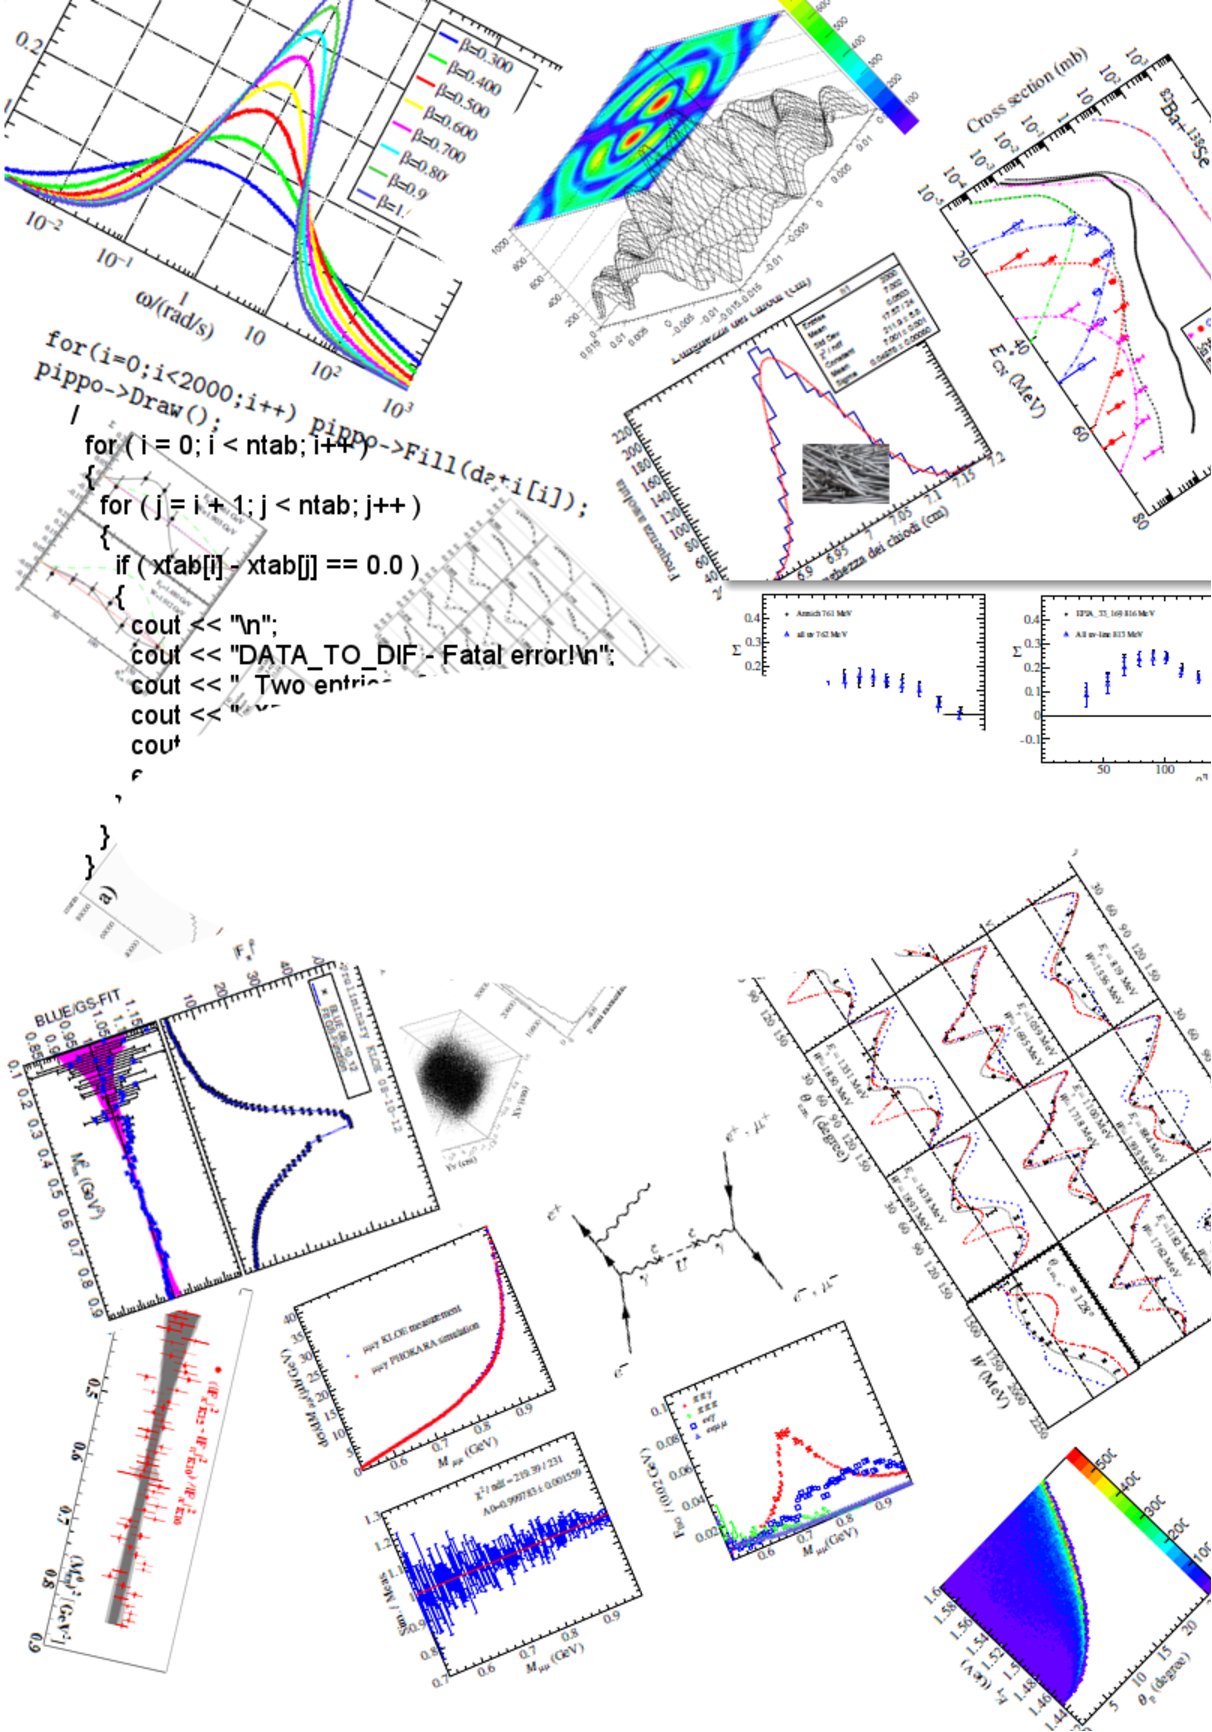
\includegraphics[width=\paperwidth]{background2}}; % Background image
\draw[anchor=north] (midpoint) node [fill=blue!10!white,fill opacity=0.8,text opacity=1,inner sep=1cm]{\Huge\centering\bfseries\sffamily\parbox[c][][t]{\paperwidth}{\centering Metodi Elaborazione Dati\\[15pt] % Book title
{\Large Appunti al corso anno accademico 2020/21}\\[20pt] % Subtitle
{\huge Giuseppe Mandaglio}\\
{\Large \it --- Dipartimento di Scienze Matematiche e Informatiche, Scienze Fisiche e Scienze della Terra --- 
Università degli Studi di Messina
}\\[5pt]
{\large \today}}}; % Author name
\end{tikzpicture}};
\end{tikzpicture}
\vfill
\endgroup

%----------------------------------------------------------------------------------------
%	COPYRIGHT PAGE
%----------------------------------------------------------------------------------------

\newpage
~\vfill
\thispagestyle{empty}

%\noindent Copyright \copyright\ 2016 Lab. Informatico CdL Fisica - Univ. Messina\\ % Copyright notice

%\noindent \textsc{Published by CdL Fisica - Univ. Messina}\\ % Publisher

\noindent \textsc{book-website.com}\\ % URL

\noindent Licensed under the Creative Commons Attribution-NonCommercial 3.0 Unported License (the ``License''). You may not use this file except in compliance with the License. You may obtain a copy of the License at \url{http://creativecommons.org/licenses/by-nc/3.0}. Unless required by applicable law or agreed to in writing, software distributed under the License is distributed on an \textsc{``as is'' basis, without warranties or conditions of any kind}, either express or implied. See the License for the specific language governing permissions and limitations under the License.\\ % License information

\noindent \textit{First printing, ??} % Printing/edition date


\newpage
%~\vfill
\thispagestyle{empty}

\noindent {\huge \bf Prefazione}
\vspace{3cm}

\noindent Il corso è ...

%----------------------------------------------------------------------------------------
%	TABLE OF CONTENTS
%----------------------------------------------------------------------------------------

%\usechapterimagefalse % If you don't want to include a chapter image, use this to toggle images off - it can be enabled later with \usechapterimagetrue

\chapterimage{chapter_head_4.pdf} % Table of contents heading image

\pagestyle{empty} % No headers

\tableofcontents % Print the table of contents itself

\cleardoublepage % Forces the first chapter to start on an odd page so it's on the right

\pagestyle{fancy} % Print headers again


\part{Linux}

\chapter{Comandi base}\index{Comandi base}

Linux è un sistema operativo libero, potente e competitivo con quelli commerciali. Esistono diverse famiglie e distribuzioni, per il corso non si consiglia una versione in particolare, l'unica avvertenza è che la versione installata sia stabile e gradita all'hardware del computer che si utilizza. Nel corso di METODI ELABORAZIONE DATI del Corso di Laurea in Fisica la distribuzione in uso è Ubuntu, le macchine sono stabili e ben manutenute.

In questo capitolo verranno descritti i comandi base per iniziare a lavorare sul terminale. Si, assolutamente si, avete letto bene lavoreremo sul terminale e il mouse e l'interfaccia grafica li utilizzeremo pochissimo. In questo momento vi state chiedendo se abbiamo intenzione di trasportarvi nel passato, ma vi assicuro che è tutto l'opposto. L'intento del corso è di portarvi nel futuro. Il passato è fatto di interfacce grafiche accattivanti che vi nascondono ciò che succede realmente nella macchina e che vi condannano all'ignoranza e alla dipendenza. Quindi un po' di fiducia e il divertimento non tarderà ad arrivare.

\section{Shell-iniziare a muoversi sulla riga di comando}\index{Shell-iniziare a muoversi sulla riga di comando}

\begin{figure}
\centering
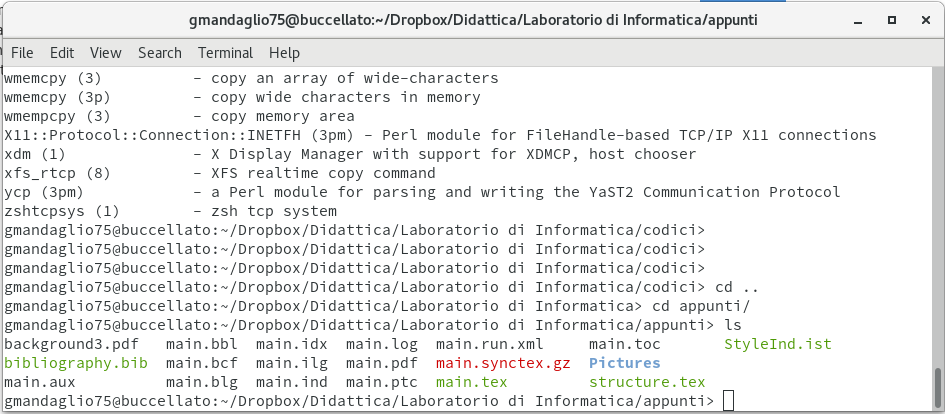
\includegraphics[scale=0.25]{scree2.png}
\caption{Dettaglio del terminale. \label{screen2}}
\end{figure}


In figura  \ref{screen2} è presente  un dettaglio del terminale dei comandi offerto da un sistema operativo di tipo Linux, in questo caso specifico si tratta di Opensuse. 
Dal terminale anche detto "shell" è possibile attraverso la chiamata diretta di una serie di comandi (programmi offerti dal sistema operativo - molti ereditati da UNIX) effettuare diverse operazioni: copiare, creare cartelle, muoversi tra le cartelle, leggere documenti, cancellare documenti o cartelle etc.


%\begin{figure}
%\centering
%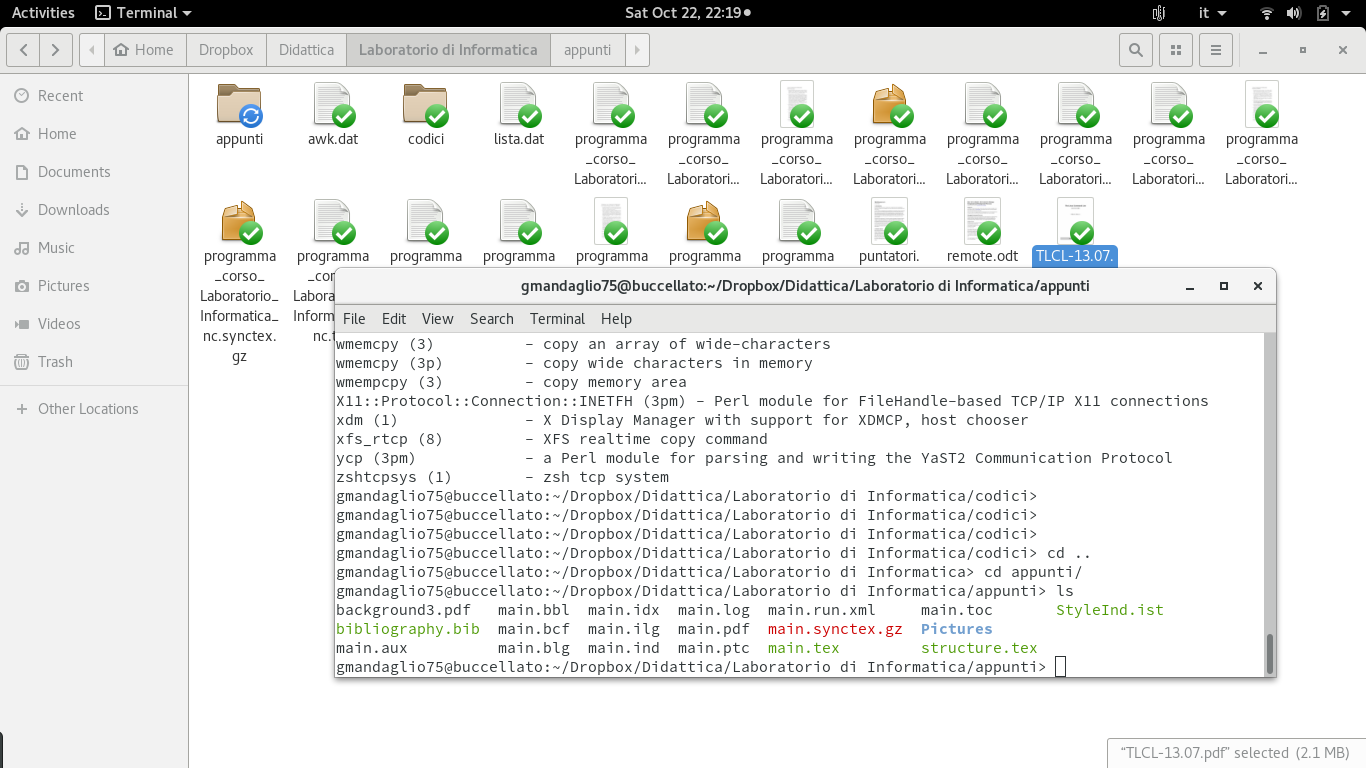
\includegraphics[scale=0.3]{screen.png}
%\caption{Foto dello schermo del pc con sistema operativo opensuse e interfaccia gnome sul quale questo manuale è in corso di scrittura. Il riquadro bianco con le scritte colorate è il terminale. \label{screen}}
%\end{figure}



Ogni comando può avere diverse opzioni, per accedere a queste opzioni bisogna scrivere di seguito il comando spazio-bianco opzione(in genere una lettera) spazio-bianco argomento-su-cui-agisce-il-comando.

Per interrogare il ``terminale'' circa le opzioni del comando è sufficiente scrivere \textbf{man} spazio-bianco nome-del-comando.

Di seguito ne elenchiamo i più comuni e frequentemente usati:
\begin{table}[h]
\begin{tabular}{cp{10cm}}
\textbf{ls} & stampa a schermo la lista dei file e delle directory contenute nella directory in cui il comando viene invocato. le opzioni -a vi fa vedere anche i file nascosti (su Linux il loro nome inizia con un punto) -l fornisce una lista dei file con più informazioni.\\
\textbf{cd} & acronimo di \textit{change directory} serve appunto a cambiare la directory corrente, a spostarsi dentro la memoria del pc. Per entrare in cartelle e sottocartelle basta separare in fase di comando i nomi delle cartelle con uno slash /. Per scendere di una cartella cd ../.\\
\textbf{cp} & serve per copiare i file. Per copiare le cartelle bisogna utilizzare 	l'opzione -r (copia ricorsiva). All'interno della stessa cartella bisogna dire al comando il nome del file da copiare e il nome della copia (che può essere differente dal nome del file da copiare) nel caso in cui si copia un file in un altro posto (secondo parametro del comando è il percorso di dove si vuole copiare il documento) il comando automaticamente creerà una copia con lo stesso nome del file di partenza.\\
\textbf{mkdir} & creare una nuova cartella (directory).\\
\textbf{rmdir} & rimuovere una cartella.\\
\textbf{rm} & rimuovere i file. Con l'opzione -r consente di cancellare cartelle e tutto ciò che contengono. Il comando rm -rf è molto potente e pericoloso, consente di cancellare file e cartelle in modo ricorsivo attraverso l'opzione r, mentre non chiede il permesso di cancellare attraverso l'opzione f (force).\\
\textbf{pwd} & vi dirà la posizione della directory corrente.\\
\textbf{chmod} & consente di cambiare i permessi dei file (lettura=r, scrittura=w esecuzione=x). Grazie a questo comando potete rendere eseguibile un documento di testo contente una serie di comandi interpretabili dal terminale che ``lanciato'' (./nomedelfile invio)  eseguirà in sequenza i comandi contenuti nel file (bash script eseguibile). chmod seguito dal meno per rimuovere il permesso, seguito dal + per conferirlo.\\
\textbf{mv} & utile per muovere i documenti da una cartella ad un'altra, oppure per cambiare il nome di un file. \\
\textbf{tar} & consente di creare file di archivio utili per conservare i propri dati o per condividerli. \\
\textbf{gzip} & consente di comprimere i file. \\
\textbf{gunzip} & consente di decomprimere i file compressi. \\
\textbf{df} & vi fornisce informazioni sullo stato della memoria del vostro pc.\\
\end{tabular}
\end{table}

Questa lista si potrebbe prolungare per diverse pagine, senza però dare mai una descrizione completa di tutte le funzionalità dei vari comandi. Il consiglio migliore per chi comincia a lavorare su un terminale unix-like tipo linux è  quello di interrogare il sistema circa le potenzialità del comando che si intende usare visualizzando a schermo il manuale del comando utilizzando la parola chiave \textit{man} nel seguente modo man-spazio-ilnomedelcomando-invio; e inoltre quello di cercare di imparare più comandi possibili ma non con la smania di un collezionista ma con la voglia di migliorare le proprie possibilità. L'unico modo per memorizzare comandi e opzioni è usarli, usarli e usarli. L'unico modo per apprenderne altri è non usare sempre le stesse cose che si conoscono ma cercare se esistono modi alternativi per fare in modo più efficiente e veloce quello che normalmente facciamo (lo so quando si ha fretta è più comodo usare ciò che si conosce, ma prima o poi ci sarà l'occasione in cui non avremo fretta: bene in quelle circostanze  bisogna cercare di essere un po' più curiosi e un po' meno pigri).

\section{Compilatori}\index{Compilatori}

I compilatori il più delle volte risultano già installati su sistemi tipo Linux oppure è possibile scaricarli gratuitamente. Sono disponibili praticamente tutti i compilatori dei linguaggi di programmazione: fortran, pascal, C, C++, perl, python, java etc.
Il linguaggio di riferimento di questo corso è il C++ e il suo compilatore si invoca attraverso il comando g++ (su mac il comando è cc e la sintassi è la stessa). Verrà inoltre utilizzato il linguaggio fortran e il compilatore di su linux è gfortran. La lettera g che precede questi compilatori sta per gnu.
La sintassi e l'utilizzo dei due compilatori è esattamente la stessa. 

Il compilatore ha il compito di tradurre il sorgente del programma (un documento di testo contenente l'implementazione del programma) scritto e comprensibile all'uomo in un file comprensibile dalla macchina che chiameremo file eseguibile o eseguibile.

Il compilatore quando viene chiamato ad analizzare un codice sorgente esegue sempre un controllo degli errori e nel caso in cui ne dovesse trovare qualcuno non completerà la compilazione, non produrrà il file eseguibile e vi mostrerà a schermo una serie di messaggi (numero di riga del codice ed errore) che vi aiuteranno ad individuare l'errore/gli errori che avete commesso (vedi fig. \ref{compilatore}).

\begin{figure}[h]
\centering
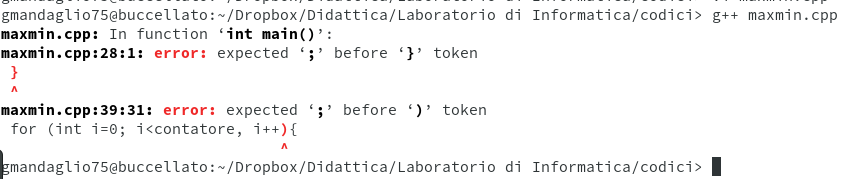
\includegraphics[scale=0.5]{compilatore.png}
\caption{Esempio di errori evidenziati dal compilatore. \label{compilatore}.}
\end{figure}




%----------------------------------------------------------------------------------------
%	PART
%----------------------------------------------------------------------------------------

\part{Programmazione in C++}

%----------------------------------------------------------------------------------------
%	CHAPTER 1
%----------------------------------------------------------------------------------------

\chapterimage{chapter_head_4.pdf} % Chapter heading image

\chapter{Introduzione}

 La programmazione è la capacità di far eseguire a una macchina una serie di istruzioni nel modo più efficiente possibile. La sequenza delle istruzioni la chiameremo \textbf{algoritmo}. La correttezza degli algoritmi, l'assenza di errori logici (bug), l'efficienza e la leggibilità del codice rappresentano l'abilità principale del programmatore.
Normalmente i programmatori informatici sono formati per implementare codici per soddisfare le esigenze di un committente (un cliente), mentre i programmatori fisici implementano codici per loro stessi o per il gruppo di ricerca con cui collaborano.  Sebbene i fisici siano molto apprezzati come programmatori e risolutori di problemi complessi, tuttavia hanno anche  la pecca di scrivere codici comprensibili solo a loro e spesso privi di qualsiasi documentazione. Quindi prima di prendere questa brutta abitudine impariamo che i codici devono essere leggibili e ben documentati in modo che anche altri li possano usare.

Riprendendo il sermone precedente notiamo che ci sono alcune parole che ci suggeriscono che per poter programmare abbiamo bisogno di alcune cose....

Alcune cose:

\textbf{Algoritmo}. Questa parola che sembra complicata, in realtà è una delle cose più comuni della nostra vita. Implementiamo
algoritmi in continuazione da sempre: alle elementari alle prese con i primi problemini di algebra pieni di contadini, uova, mercatini etc; quando cuciniamo una frittata; quando guidiamo la macchina; quando scriviamo un messaggio sul cellulare etc. Creiamo algoritmi in continuazione
creiamo una sequenza di azioni atte a risolvere un problema o a fare una azione e in questi casi il pc normalmente siamo noi stessi.

Purtroppo il pc non possiede un cervello come il nostro e non può risolvere i problemi al posto nostro.
Si, purtroppo è così!!! I problemi li dobbiamo risolvere noi. Il pc però è veloce, straordinariamente veloce.

Il pc parla una sua lingua e noi ne parliamo un'altra; come possiamo fare a comunicare le nostre idee geniali in modo che il pc possa aiutarci a risolvere il dato problema??

Ci serve un interprete che traduca i nostri codici in un linguaggio comprensibile alla macchina, un linguaggio con delle regole e degli strumenti che ci consentano di implementare i nostri algoritmi.

I compilatori o gli interpreti sono dei programmi che hanno il compito di tradurre i nostri codici (codice sorgente) in linguaggio macchina. 
I compilatori traducono interamente il codice sorgente in codice macchina comprensibile ed eseguibile dal pc, mentre gli interpreti traducono e fanno eseguire al pc una istruzione alla volta. I codici sorgente eseguiti da un interpretate sono molto più lenti, in genere sono di piccole dimensioni e facilmente manutenibili e forniscono completo accesso al codice. Quelli compilati sono invece molto veloci perché eseguibili per intero senza ulteriori traduzioni, non hanno bisogno dei codici sorgenti ne dell'interprete (si può nascondere il sorgente), tuttavia per rimediare ad un errore all'interno del codice è necessario ricompilare il programma e in progetti di grosse dimensioni può richiedere una certa quantità di tempo.


I compilatori hanno capacità di diagnostica sulla correttezza sintattica del codice, vi informano degli errori e non procedono alla creazione un programma eseguibile finché il codice sorgente non viene corretto da tutti gli errori di sintassi. 
Il compilatore non ci rende immuni dagli errori di logica, quindi scrivere codici corretti è condizione necessaria ma non sufficiente alla risoluzione di un problema con un codice. L'errore più grave che può commettere un programmatore inesperto è subordinare la logica del programma all'esigenza di portare a buon fine un processo di compilazione: sentire pronunciare espressioni del tipo ``ho spostato questo frammento di codice perché non compilava'' nuoce gravemente la salute di chi ascolta ( o nei casi meno gravi può causare una certa acidità di stomaco) quindi dire cose del genere è moralmente deplorevole.

Nel presente corso il linguaggio eletto allo scopo è il C++, la scelta ha svariate ragioni: è un linguaggio a basso e alto livello, consente di strutturare i programmi in modo che siano orientati agli oggetti, è il linguaggio con il quale sono implementati sistemi operativi, linguaggi ad alto livello come ad esempio python. Si presta bene per imparare a programmare in modo procedurale ed ovviamente orientato agli oggetti.

Alcune lezioni saranno spese per imparare a tradurre i codici procedurali implementati in C++/C in linguaggio Fortran. Il Fortran
è un linguaggio molto potente e rivolto al calcolo scientifico. Conoscere la sua sintassi è di grande utilità per poter accedere al patrimonio immenso di codici scritti in questo linguaggio dalla comunità dei fisici e ancora diffusamente utilizzati.

Alla fine del corso, una introduzione alle tecniche fondamentali per l'analisi dei dati verrà affrontata utilizzando il framework root, e il programma gnuplot.


Il corso suggerisce caldamente l'utilizzo di un pc con sistema operativo Linux (qualunque distribuzione va bene), o comunque un sistema operativo tipo Unix. Su linux il compilatore (libero) che verrà utilizzato è g++.

\section{Stuttura di un programma}\index{Stuttura di un programma}

Di seguito il listato di un semplicissimo programma in C++
che una volta compilato ed eseguito attraverso la sua versione
eseguibile dal pc stampa a monitor la stringa di caratteri ``Ciaooooooo!''.

\begin{verbatim}
//con il doppio slash inseriamo commenti nel programma
//i commenti sono ignorati dal compilatore
//i commenti sono utili per rendere più leggibile il codice
// Il primo programma in C++
#include <iostream>// include la libreria iostream

int main()
{
  std::cout << "Ciaooooooo!";
  return 0;
}
\end{verbatim}

Per compilare questo codice bisogna che esso sia trascritto in un file con estensione cpp (utile perché ci dice che abbiamo a che fare con un codice sorgente di tipo C++ e inoltre informa i programmi di editor del tipo di file in questione e l'editor colora in modo molto utile le righe del codice aiutandoci nella programmazione).
Poi su un Linux da riga di comando si digita :\\
g++ nomedelsorgente.cpp\\
il compilatore g++ per default crea il file a.out che contiene il nostro eseguibile. Per eseguire il programma bisogna digitare sul terminale il comando
 \begin{verbatim}
./a.out
\end{verbatim}
e poi fare invio.

Ogni volta che eseguiamo una compilazione in questo modo, g++ sovrascriverà il file a.out con il nuovo eseguibile e quindi il vecchio sarà perso. Se invece si vuole conservare una copia dell'eseguibile può essere utile utilizzare l'opzione di g++ che consente di decidere il nome dell'eseguibile.\\
g++ -o nome\_eseguibile sorgente.cpp (la lettera o sta per output della compilazione) 


All'interno del codice sorgente è possibile scrivere dei commenti che sono riservati al programmatore e che non vengono interpretati dal compilatore. I commenti sono preceduti da un doppio slash. I commenti sono molto utili a rendere il codice più leggibile e forniscono una breve documentazione al codice.  

Procediamo a commentare il programma riga per riga:
prima di ogni cosa troviamo una istruzione che inizia con carattere cancelletto e che segue con il comando include. Questa istruzione serve a dire al preprocessore del compilatore che deve appunto includere nel programma la libreria \textbf{iostream}. Senza l'inclusione della libreria \textbf{iostream} che contiene le funzionalità di input-output non avremmo potuto utilizzare il comando std::cout << "Ciaooooooo!"; e stampare a schermo la stringa "Ciaooooooo!".

Inclusa la libreria, il programma definisce la funzione principale. In C++/C qualunque programma non può prescindere dalla funzione principale, in questo linguaggio tutte le procedure sono funzioni e la funzione che ha il nome main è una funzione speciale e come già detto la più importante. La funzione main ha il compito di coordinare il funzionamento del programma. 
Usiamo la funzione \textbf{main} per introdurre la struttura di una funzione.

\textbf{Ogni istruzione} deve essere chiusa con \textbf{un punto e virgola} ad eccezione dell'inclusione delle librerie o quando raggruppiamo istruzioni utilizzando le parentisi graffe.

\begin{verbatim}
// int è il tipo di valore che la funzione restituisce
// se la funzione non restituisce nulla si può mettere void al posto di int
// all'interno delle parentesi ci sono le variabili che riceve
//possono essere di diverso tipo come nell'esempio
//oppure non esserci nulla, la funzione non riceve nulla
int nomefunzione (int a, float b, double c, ...etc) 
	{
	//all'interno delle graffe ci sono le istruzioni
	istruzione 1;
	// tutte le istruzioni chiudono con un punto e virgola
	// eccetto l'istruzione #include
	istruzione 2;
	.....etc;
	//alla fine dell'esecuzione, o al suo interno
	// l'operazione return restituisce un valore
	// del tipo dichiarato ed esce dalla funzione
	// se la funzione in questione è la funzione
	// principale il programma termina
	// se è una funzione qualunque restituisce il dato valore
	// alla funzione principale e il programma continua a "girare".
	return variabile_che_restituisce;
	} 
\end{verbatim}


Ritorniamo al programma, l'istruzione  $std::cout << "Ciaooooooo!";$
utilizza la classe \textbf{cout} della libreria \textbf{iostream} per stampare a schermo la frase $"Ciaooooooo!"$. L'operatore minore-minore $<<$ dice che la stringa $"Ciaooooooo!"$, definita attraverso le virgolette (senza virgolette Ciaooooooo sarebbe una variabile) dal programmatore viene data in input al programma \textbf{cout} e il programma \textbf{cout} lo stampa sullo schermo.

\textbf{cout} è un oggetto che ci consente di scrivere sullo schermo, possiamo scrivere parole o frasi scrivendole tra virgolette, oppure variabili
e in questo caso il valore della variabile sarà stampata a schermo.
es.

\begin{verbatim}
std::cout << "il valore del nostro calcolo e' = "<< valore<<"\n";
\end{verbatim} 

Nell'esempio, \textbf{cout} stamperà a monitor se valore fosse uguale a 1.23\\
il valore del nostro calcolo è = 1.23\\
e poi sarebbe andato a capo perché abbiamo messo il comando tra virgolette slash n (al posto di questo comando si sarebbe ottenuto lo stesso effetto utilizzando l'espressione \textbf{endl}). Se non chiediamo a \textbf{cout} di andare a capo, \textbf{cout} non lo farà automaticamente e scritture multiple appariranno a schermo sulla stessa riga.

Includendo tra le inclusioni delle varie librerie $\#include$ e la funzione principale il comando:\\
using manespace std;\\
si evita il bisogno di scrivere davanti ai membri della libreria il prefisso $std::$.


I programmi vengono eseguiti in modo sequenziale dalla prima all'ultima istruzione, quindi leviamoci dalla testa che il seguente pezzo di codice possa restituire il valore 5:

\begin{verbatim}
int a,b,c;
c=a+b;
a=2;
b=3;
cout<<"non restituisce 5 manco se ti metti a piangere :P  ="<< c <<endl;
\end{verbatim} 

il codice corretto sarebbe:

\begin{verbatim}
int a,b,c;
a=2;
b=3;
c=a+b;
cout<<"grazie così va bene, la somma di a e b è  ="<< c <<endl;
\end{verbatim} 
 

\section{Operazioni di input-output I}\index{Operazioni di input-output I}

Il programma seguente lo utilizziamo per introdurre l'uso delle variabili. Nell'esempio le variabili si chiamano a,b, e results e sono tutte variabili di tipo intero. Il programma assegna i valori alle due variabili (5 e 2), poi somma la quantità 1 alla variabile a e poi fa la differenza tra a e b e assegna questo valore alla variabile result, infine stampa a monitor il risultato della differenza attraverso la variabile result.
\begin{lstlisting}[language=c++]

// operating with variables

#include <iostream>
using namespace std;

int main ()
{
  // declaring variables:
  int a, b;
  int result;

  // process:
  a = 5;
  b = 2;
  a = a + 1;
  result = a - b;

  // print out the result:
  cout << result;

  // terminate the program:
  return 0;
}
\end{lstlisting}


Ora immaginiamo di voler confezionare un programma capace di chiedere ad un utente di fornirgli da riga di comando due numeri, e lui in cambio li somma e restituisce a schermo il risultato. Per fare questo ci serve un qualche cosa che operi al contrario di \textbf{cout}. Il metodo che fa al nostro scopo è \textbf{cin}. \textbf{cin} funziona sintatticamente in modo equivalente a \textbf{cout} solo che i minore-minore si trasformano in maggiore-maggiore ad indicare che \textbf{cin} prende qualche cosa dal terminale e lo assegna ad una variabile nel programma.
In pratica \textbf{cin} e \textbf{cout} si comportano come due messaggeri che fanno parlare il mondo del programma con quello esterno del terminale.
Più avanti presenteremo anche i loro fratelli omologhi del C printf e scanf, utilizzabili nel C++ che assorbe completamente C.\\
es. \textbf{cin>>variabile;} //assegna ad variabile il valore digitato al terminale dopo l'invio\\
es. \textbf{cin>>variabile1>>variabile2; }// in questo caso due valori. Per passarli a \textbf{cin}, abbiamo due strade, digitiamo un valore poi invio e così per il secondo oppure digitiamo entrambi i valori separati da uno spazio bianco e poi invio.

\begin{lstlisting}[language=c++]

// operating with variables

#include <iostream>
using namespace std;

int main ()
{
  // declaring variables:
  int a, b;
  int result;

  // process:
  cout << "potresti darmi un numero?"<<endl;
  //endl e' un modo alternativo per andare a capo
  cin  >> a;
  cout << "potresti darmi un'altro numero?"<<endl; 
  cin >> b;
  cout << "Grazie!"<<endl;
  
  result = a + b;

  // print out the result:
  cout << "ecco il risultato della somma =" <<result<<endl;
  cout << "ecco il prodotto occhio al codice ="<< a*b<<endl;

  // terminate the program:
  return 0; 
}
\end{lstlisting}

\chapter{Elementi base per la programmazione}\index{Programmazione procedurale}

\section{Variabili I}\index{Variabili I}
Le variabili in qualunque linguaggio di programmazione possono essere di diverso tipo: intere, reali, complesse, caratteri, stringhe (insiemi di caratteri) etc. Le variabili vanno sempre dichiarate, questa operazione è fondamentale perché bisogna prenotare le locazioni di memoria capaci di ospitare il dato. Se le variabili non vengono dichiarate il compilatore segnalerà la cosa come un errore: il C++/C non sono dotati di un sistema automatico di assegnazione delle variabili (python ad esempio è dotato di un sistema di assegnamento automatico, ma python è un linguaggio ad alto livello e tutto quello che ci risparmia è dovuto a implementazioni che fanno il lavoro al posto nostro. Python è implementato in c++).

Il codice seguente:\\
\begin{lstlisting}[language=c++]
#include <iostream>// include la libreria iostream

int main()
{
  pi_greco=3.14;
  return 0;
}
\end{lstlisting}

produrrebbe il seguente errore in fase di compilazione 



\begin{verbatim}
gmandaglio75@buccellato:~> g++ prova.cpp
prova.cpp: In function ‘int main()’:
prova.cpp:6:3: error: ‘pi_greco’ was not declared in this scope
   pi_greco=3.14;
   ^~~~~~~~
\end{verbatim}



\begin{table}[h]
\footnotesize
\begin{tabular}{c|c|c}
Gruppi & Tipi di carattere & note\\
\hline
          & char	    & 1 byte, almeno 8 bits\\
Caratteri & char16\_t	&   non più piccolo di un Char, almeno 16 bits.\\
          & char32\_t	& non più piccolo di un char16\_t, almeno 32 bits.\\
          & wchar\_t	    & il più grande tipo di carattere supportato.\\
          \hline
          

 & signed int	          & da  -2147483648 a   2147483648 (32 bit)\\
Tipo intero con segno & signed long int	      & da  -2147483648 a   2147483648\\
 & signed long long int  & da -9223372036854775808 a 9223372036854775808\\
\hline
	& float	& da 1.17549$\times 10^{-38}$ a 3.40282$\times 10^{+38}$\\
Tipo reale  &  double &	 da 2.22507$\times 10^{-308}$a 1.79769$\times 10^{+308}$\\
   & long double &	da  3.3621$\times 10^{-4932}$ a 1.18973$\times 10^{+4932}$\\
\hline
Tipo Booleana &	bool &	assume i valori 1 - 0 o ``true'' - ``false''\\
\hline
Tipo vuoto &	void &	nessuno spazio di memoria occupato
\end{tabular}
\caption{ Lista di variabili disponibili in C++, nome e dimensioni. \label{tab1}}
\end{table}

Come si può vedere in tabella \ref{tab1} ci sono diversi tipi di variabile che possono essere utilizzate dentro i nostri codici. \'E importante notare che la grandezza delle variabili è considerevole nelle variabili di tipo \textit{long}, ma non infinita. Il concetto di infinito è per gli esseri umani non per le macchine. 






\section{Operatori}\index{Operatori}

\subsection{Assegnazione =}\index{Assegnazione =}

L'operatore di assegnazione è =. Lo abbiamo già utilizzato negli esempi precedenti. \'E importante sottolineare che questo operatore esegue solo l'operazione di assegnazione ovunque esso venga invocato, non comparazione, non risponde a nessuna domanda! Scrivere che a=b; o a =25; significa che la variabile a assumerà lo stesso valore della variabile b oppure il valore 25 nel secondo caso.

\subsection{Operatori aritmetici ( +, -, *, /,\% )}\index{Operatori aritmetici ( +, -, *, /,\% )}

Gli operatori somma, sottrazione, prodotto(simbolo asterisco *), divisione (simbolo slash /), e modulo (simbolo \%) ci consentono di lavorare su numeri e variabili. Bisogna ricordarsi che gli operatori obbediscono ad un ordine gerarchico che d\'a a prodotto/divisione/modulo priorità di esecuzione sulle operazioni di somma e sottrazione. Quindi la variabile pippo nel seguente frammento di codice assumerà il valore 11 piuttosto che 21.
\begin{verbatim}
int pippo = 5 + 2 * 3;
\end{verbatim}

L'operatore modulo \% restituisce il resto della divisione tra due numeri.
Questa operazione è molto utile se vogliamo stabilire se un numero intero memorizzato in una variabile sia pari o dispari, per fare questo basta verificare se il valore restituito dall'operazione variabili\%2 sia pari a zero (pari) o a 1 (dispari).\\





\subsection{Operatori di assegnazione composti (+=, -=,*=,/=)}\index{Operatori di assegnazione composti (+=, -=,*=,/=)}%    <<=, \&=,  \|=)}


In C++ è possibile comporre gli operatori di assegnazione con altri creando delle scritture abbreviate come nella tabella seguente:
\begin{table}[h]
\centering
\begin{tabular}{c|c}
espressione	& equivalente a...\\
\hline
y += x; &	y = y + x;\\
\hline
x -= 5;	& x = x - 5;\\
\hline
x /= y;	& x = x / y;\\
\hline
x *= y;	& x = x * y;\\
\end{tabular}
\caption{Equivalenza tra assegnazioni composte. \label{tab2}}
\end{table}
\subsection{Operatori di incremento e decremento}\index{Operatori di incremento e decremento}

Gli operatori ++ e $--$ sono detti operatori di incremento e di decremento, nel senso che aumentano o diminuiscono di una unità la variabile alla quale vengono applicate.
\begin{verbatim}
x++; // equivale a x = x +1;
x--; // equivale a x = x -1;
\end{verbatim}
é importante notare il verso dell'applicazione dell'operatore nel caso in esso venga utilizzato nelle espressioni:
\begin{verbatim}
x=20; // 
y = x++; // in questo caso y è uguale 20 e x a 21
//mentre!!!!!!!!!!
y = ++x;  //in questo caso y e x sono uguali a 21
\end{verbatim}

Nel primo caso prima viene effettuata l'operazione di uguaglianza e poi quella di incremento producendo una differenza tra le due quantità alla fine dell'operazione, nel secondo caso invece prima si incrementa e poi si eguaglia.

\subsection{Operatori di comparazione}\index{Operatori di comparazione}
Gli operatori di comparazione ci aiutano a stabilire la veridicità di una comparazione tra variabili e grandezze. Se la relazione scritta è soddisfatta restituirà il valore \textit{vero} altrimenti il valore \textit{falso}. Queste espressioni saranno di fondamentale importanza per le strutture di controllo e per il ciclo \textit{while} che vederemo in seguito.
\begin{table}[h]
\centering
\begin{tabular}{c|c}
 operatore &	descrizione\\
 \hline
$==$ &	Uguale\\
 \hline
!= &	Diverso\\
 \hline
$<$ &	Minore di\\
 \hline
$>$ &	Maggiore di\\
 \hline
$<=$ &	Minore uguale a \\
 \hline
$>=$ &	Maggiore uguale a\\
\end{tabular}
\caption{Operatori di comparazione. \label{taboc}}
\end{table}
\subsection{Operatori di logici}\index{Operatori di logici}

Gli operatori logici ci consentono di combinare delle condizioni, e a seconda della loro veridicità restituiranno un valore vero o falso. L'operatore OR è realizzato legando due condizioni con un \textit{doppio pipe} mentre la condizione AND con una \textit{doppia e commerciale}, mentre la negazione è ottenuta con il punto esclamativo.
\begin{table}[h]
\centering
\begin{tabular}{c|c}
 operatore &	descrizione\\
 \hline
\&\& &	AND\\
 \hline
|| &	OR\\
 \hline
! &	NOR\\
\end{tabular}
\caption{Operatori di logici principali. \label{tabok}}
\end{table}

L'operatore \textbf{AND} restituisce un valore vero se e soltanto se entrambe le condizioni sono vere, mentre l'\textbf{OR} restituisce vero se almeno una delle due condizioni è vera.





\section{Strutture di controllo}

Le strutture di controllo ci consentono di inserire nei nostri programmi la possibilità di scegliere se eseguire alcune istruzioni oppure altre a seconda della veridicità di una condizione.
La condizione può essere una variabile logica booleana, o una espressione composta con gli operatori di comparazione, oppure il valore (0 o 1) restituito da qualcuno (va bene, va bene, non vi seccate: questo qualcuno potrebbe essere una classe o una funzione ma lo vedremo in seguito).
Le parole chiave che ci consentono di attivare una tale struttura sono \textbf{if} ed \textbf{else}, la prima significa \textbf{se} mentre la seconda \textbf{altrimenti}. L'opzione \textbf{else} non è obbligatoria, e se non si usa l'istruzione \textbf{if} porrà condizione alla istruzione o all'insieme di istruzioni racchiuse tra graffe che la seguono.
Se dopo l'\textbf{if} o dopo l'\textbf{else} se si vuole far seguire una sola istruzione allora in questo caso le parentesi graffe possono essere omesse. La condizione controllata dall'\textbf{if} deve essere racchiusa tra parentesi tonde, mentre l'\textbf{else} eseguendo ciò che la segue se la condizione dell'\textbf{if} non è "vera" non ha bisogno di una sua condizione tra parentesi tonde.

\begin{verbatim}
\\struttura del costrutto if ... else

if(condizione) {
istruzione 1;
istruzione 2;
....

istruzione n;
}
else{
Istruzione 1;
Istruzione 2;
....

Istruzione n;
}
\end{verbatim}


Un primo esempio semplice, che richiama l'uso dell'operatore modulo \% è quello di determinare se un numero dentro un codice sia pari o dispari.

esempio:
\begin{verbatim}
int pippo;
.....
......
....... (a un certo punto pippo assumerà un valore)

if(pippo%2==0)
cout<<"pippo è pari";
else
cout<<"pippo è dispari";
\end{verbatim}




Un secondo esempio, familiare a masticatori di numeri come i fisici è quello in cui si vuole indicare l'interno di un intervallo oppure il suo esterno. Un caso molto semplice che possiamo considerare è quello di un intervallo fissato da due valori su un asse di un sistema di riferimento cartesiano. Grazie a questo esempio possiamo esercitarci con la struttura di controllo e nel definire la condizione della struttura con gli operatori di confronto e gli operatori logici. 
L'esempio può essere formulato in modo equivalente utilizzando l'operatore \textbf{AND} (che individua l'interno) oppure l'\textbf{OR} (che individua l'esterno).\\
esempio \textbf{AND}: 
\begin{verbatim}
// immaginiamo su un ascissa un intervallo tra i valori 2 e 7
float x;
....
.....
....
if((x>=2) && (x<=7))
cout<< "x è interno all'intervallo"<<endl;
else
cout<< "x è esterno all'intervallo"<<endl;
\end{verbatim}
 
esempio \textbf{OR}: 
\begin{verbatim}
// immaginiamo su un ascissa un intervallo tra i valori 2 e 7
float x;
....
.....
....
if((x<2) || (x>7))
cout<< "x è esterno all'intervallo"<<endl;
else
cout<< "x è interno all'intervallo"<<endl;
\end{verbatim}

\section{Cicli:  while, do ...while,for}\index{Cicli: for, while, do ...while}

Nella programmazione una operazione molto utile e ricorrente è quella di ripetere una istruzione o un gruppo di istruzioni un certo numero di volte. 

Un esempio molto semplice che ci può aiutare a comprendere l'utilità dei cicli è l'operazione di somma. \'E vero che se dobbiamo sommare due numeri non è un grande problema, e neanche se fossero 10 se invece fossero 20 sarebbe orribilmente noioso ma ce la potremmo fare ma se le quantità che dobbiamo sommare fossero 100, o 1000 o 1000000 etc. In questo caso il modo più semplice per non scrivere una istruzione lunga un chilometro, e cavarsela con poche righe di codice  è ricorrere a un ciclo.
L'istruzione potrebbe consistere di una operazione che somma un addendo alla volta e lo accumuli in una variabile contenitore inizializzata a zero (elemento neutro dell'operazione di somma) prima dell'inizio del ciclo.

Come esempio implementeremo un programma che ci chiede il voto che abbiamo conseguito in tutti i corsi che abbiamo superato e una volta che abbiamo finito di darglieli ci restituirà la media:

\begin{lstlisting}[language=c++]
// operating with variables

#include <iostream>
using namespace std;

int main ()
{
  // declaring variables:
  float somma, voto;
  int n_materie_superate = 0;
   somma = 0;
  
  cout << "questo programma calcola la media"<<endl;
  cout << "dei voti che hai conseguito"<<endl;
  voto=1; //per innescare il ciclo while
  while (voto > 0){
  cout << "dimmi il voto o scrivi 0 per chiudere"<<endl;
  cin  >> voto;
  if( voto > 0)
  {
   somma = somma + voto ; // avremmo potuto scrivere somma + = voto;
   n_materie_superate++; // incrementiamo di una unita'
  }
  }
  // print out the result:
  cout << "La tua media e' =" <<somma /n_materie_superate <<endl;
  return 0; 
}
\end{lstlisting} 

Nell'esempio precedente abbiamo implementato un ciclo utilizzando il costrutto del \textbf{while}, questa parola significa \textit{finchè}e consente di ripetere le istruzioni che lo seguono finché la condizione contenuta tra le parentesi tonde che lo seguono è soddisfatta (o in altre parole è vera). Il ciclo \textbf{while} consente di costruire cicli che non si conosce a-priori la durata, e come abbiamo visto nell'esempio precedente abbiamo avuto bisogno di un "innesco" che consentisse al ciclo di partire. Una volta partito, le sorti del ciclo dipendono dalle istruzioni che lo seguono. Questo costrutto è molto potente, e come dice lo zio dell'Uomo Ragno "da grandi poteri discendono grandi responsabilità" e quindi è anche molto pericoloso. A parte gli scherzi, se il \textbf{while} non è implementato in modo corretto può trasformarsi in un ciclo infinito dal quale non è possibile uscire.

Se volessimo ovviare al problema dell'innesco potremmo usare il costrutto \textbf{do-while} il quale in ogni caso almeno una volta eseguirà le istruzioni che il costrutto contiene:

\begin{verbatim}
do{
istruzione 1;
istruzione 2;
....
....
....
}while(condizione)
\end{verbatim}

Se invece vogliamo implementare un ciclo e conosciamo a-priori il numero di volte che lo vogliamo ripetere, allora in questo caso possiamo utilizzare il costrutto del \textbf{for}. Il costrutto del ciclo è il seguente:


\begin{verbatim}
for(int indice; indice< fine; indice++){
istruzione 1;
istruzione 2;
....

....
....
}
\end{verbatim}
Anche per il \textbf{for} se l'istruzione che si deve ripetere è una sola si possono omettere le parentesi graffe, tuttavia per ragioni legate alla leggibilità e alla manutenibilità del codice è \textbf{buona educazione} mettere sempre le parentesi graffe anche nei casi in cui si possono omettere. La disinvoltura nel rimuoverle quando è possibile farlo crea codici meno leggibili e che in caso di modifica spesse volte presentano errori di logica. Nel presente testo si cercherà di non violare mai questa buona regola di scrittura del codice, nel caso accadesse prego a chiunque lo noti di segnalarmelo.

Le implementazioni dei cicli sono equivalenti tra di loro. Nell'esempio che segue il codice stampa a schermo i numeri da 0 a 9 utilizzando in modo equivalente i due costrutti.

\begin{verbatim}

for(int i =0 ; i<10; i++) cout<<i<<endl;
//oppure
int i =0;
while(i<10){cout<<i<<endl; i++;}
\end{verbatim}

Un esempio di utilizzo del ciclo \textbf{for} utile quando si vuole generare una sequenza di numeri è dato dal seguente codice che stampa a schermo 20 valori a passo costante da 0 a 3.14.

\begin{lstlisting}[language=c++]
#include <iostream>
#include <cmath>
using namespace std;

main (){
float pi=3.14;
float n=0;
cout<<"Sequenza dei numeri da 0 a pi-greco"<<endl;
for(int i=0; i<20; i++){
n=n+(pi/20);
cout<<n<<endl;
}
return 0;
}
\end{lstlisting}




\section{Esercitazioni - Algoritmi}\index{Esercitazioni - Algoritmi}


\subsection{Integrale di una funzione con il metodo dei rettangoli}\index{Integrale di una funzione con il metodo dei rettangoli}

In questo paragrafo utilizzeremo un esercizio svolto in classe per fare un po' di riassunto delle cose finora apprese. L'esercizio
consiste nel calcolare l'integrale della funzione $f(x) = x^2$ nell'intervallo tra 0 e 5 con il metodo numerico dei rettangoli.
Questo metodo numerico è probabilmente il più semplice per stimare numericamente un integrale definito. Esso consiste nell'approssimare l'area sottesa alla curva con la somma dei rettangoli costruiti in modo che la loro base sia pari all'intervallo di integrazione diviso per il numero di divisioni che vogliamo utilizzare per il calcolo e la loro altezza sia pari al valore assunto dalla funzione nel valore medio del sotto intervallo in considerazione.
In Figura \ref{rettangoli} sono rappresentati la curva in questione e i rettangoli costruiti per 10, 20, 30, 40 divisioni dell'intervallo di integrazione. Dalla figura intuiamo che all'aumentare del numero di divisioni aumenta la precisione dell'integrale.
Come funziona questo metodo? L'idea di base consiste nel fatto che l'area del rettangolo rappresenta una buona stima di quella ottenuta sostituendo alla base superiore del rettangolo la curva descritta dalla funzione. Se poniamo attenzione all'intersezione tra curva e rettangolo notiamo la formazione di due  figure simili a ``triangoli'', uno superiore alla curva che introduce una sovrastima all'area e uno inferiore che la sottostima. L'algoritmo sfrutta il fatto che queste due aree si compensano.

\begin{figure}[h]
\centering
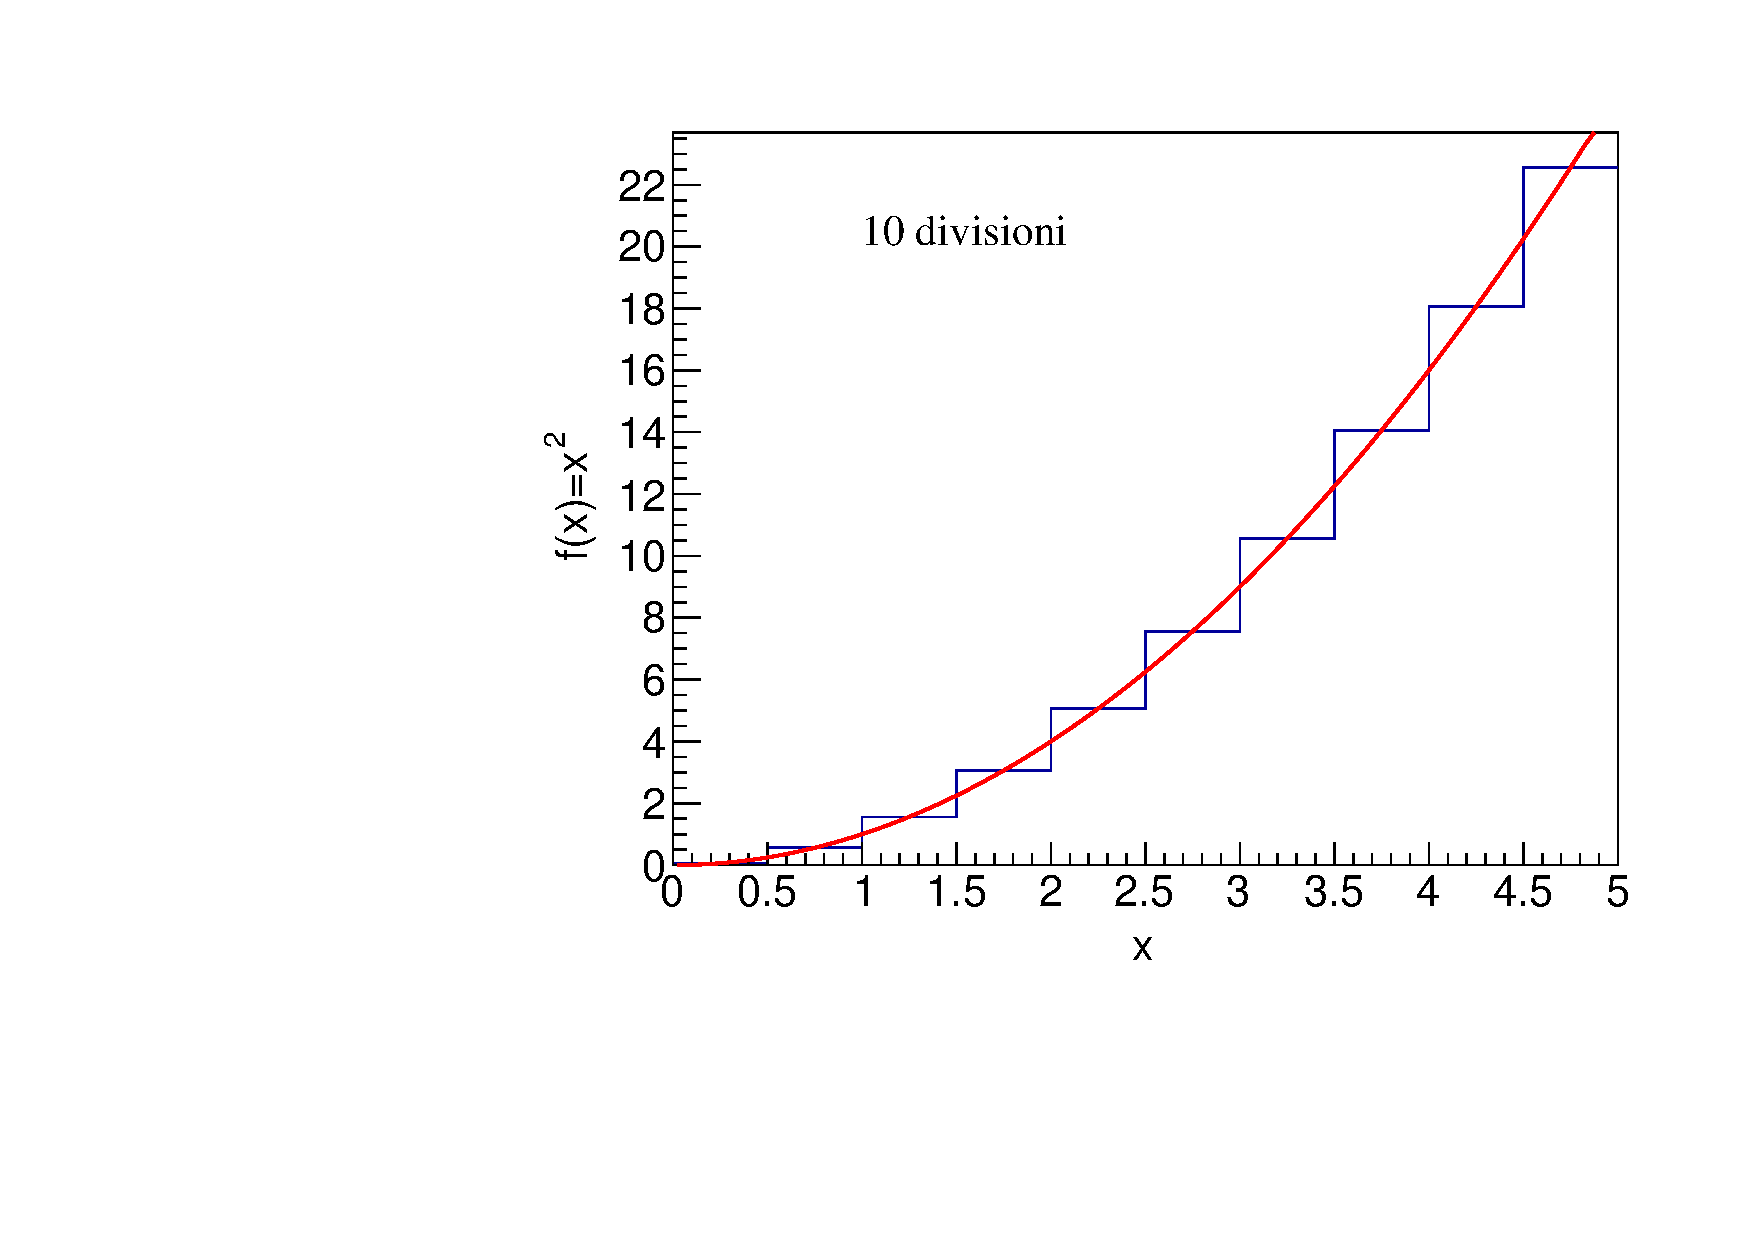
\includegraphics[scale=0.3]{./Pictures/intpar10.pdf}
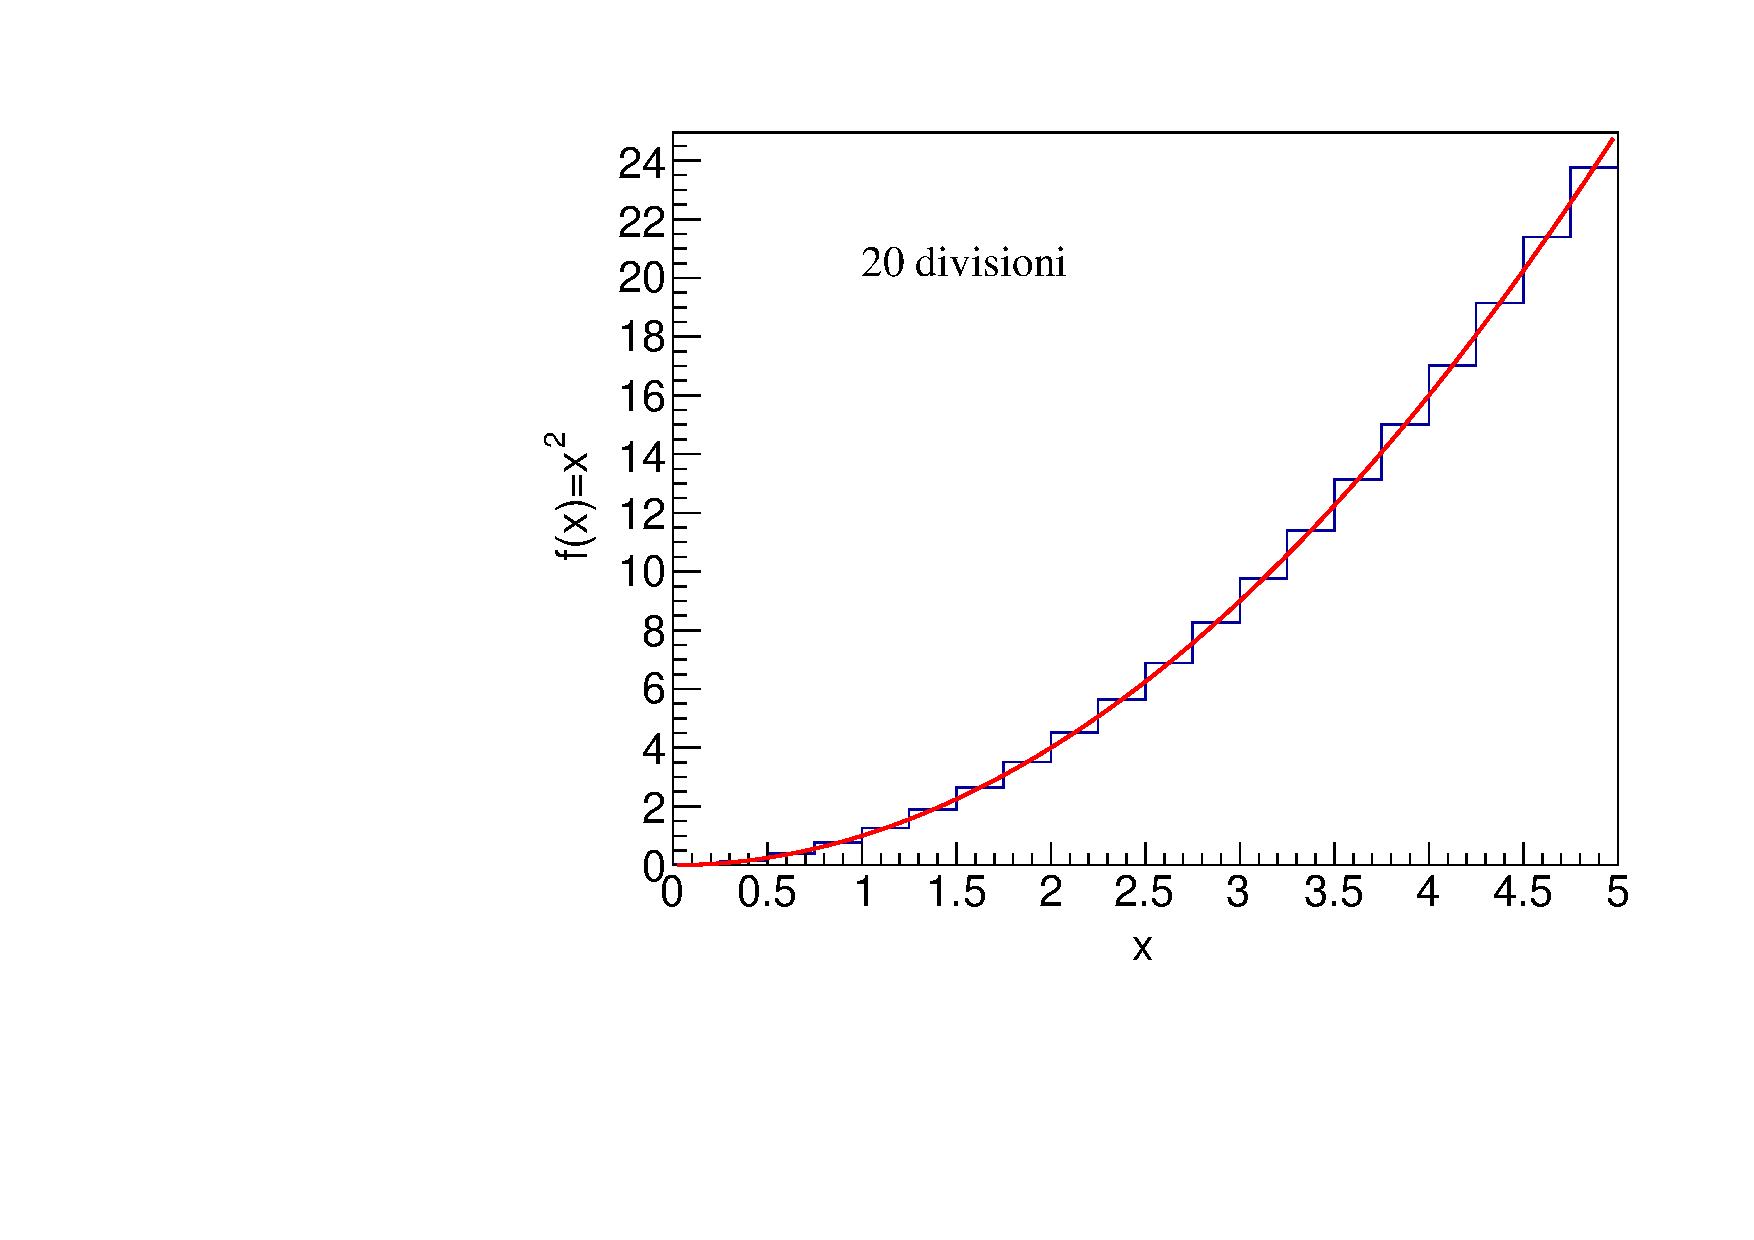
\includegraphics[scale=0.3]{./Pictures/intpar20.pdf}\\
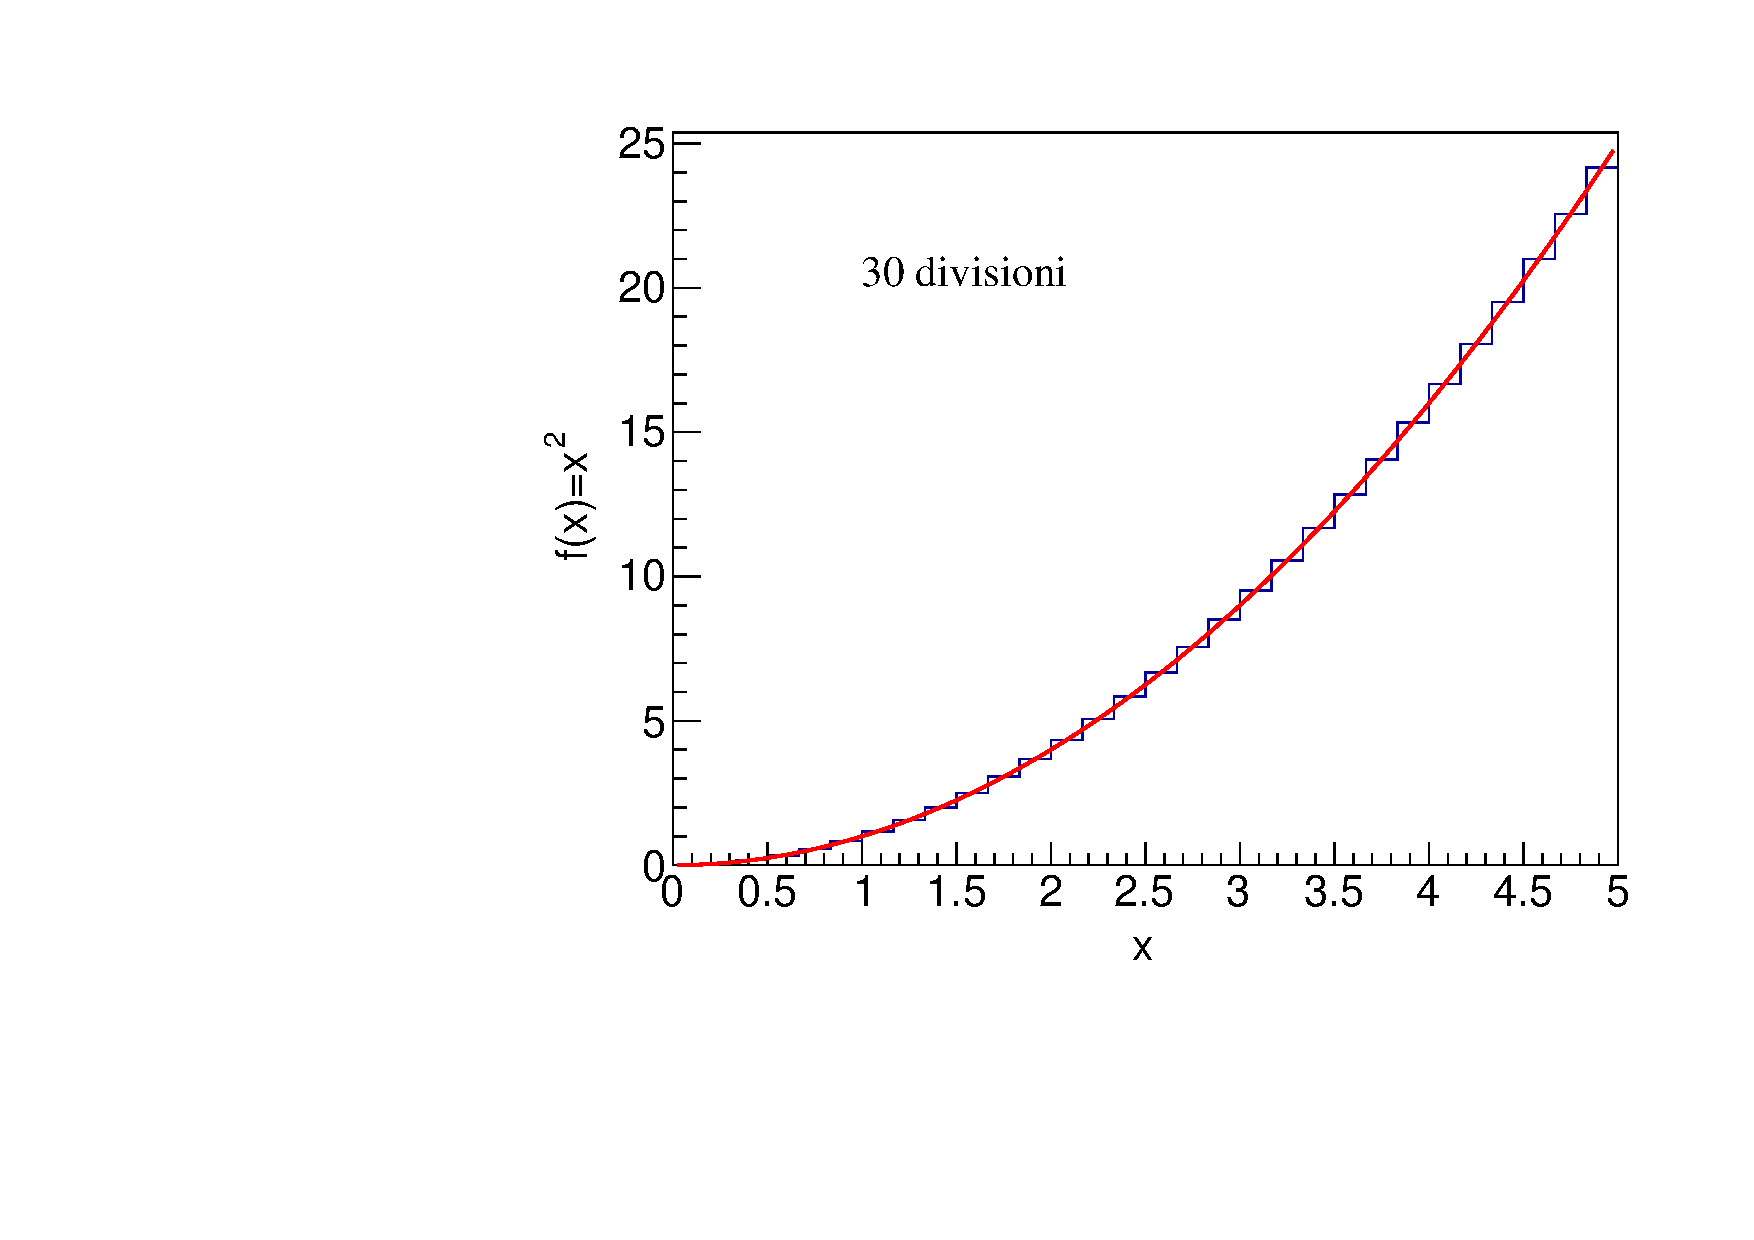
\includegraphics[scale=0.3]{./Pictures/intpar30.pdf}
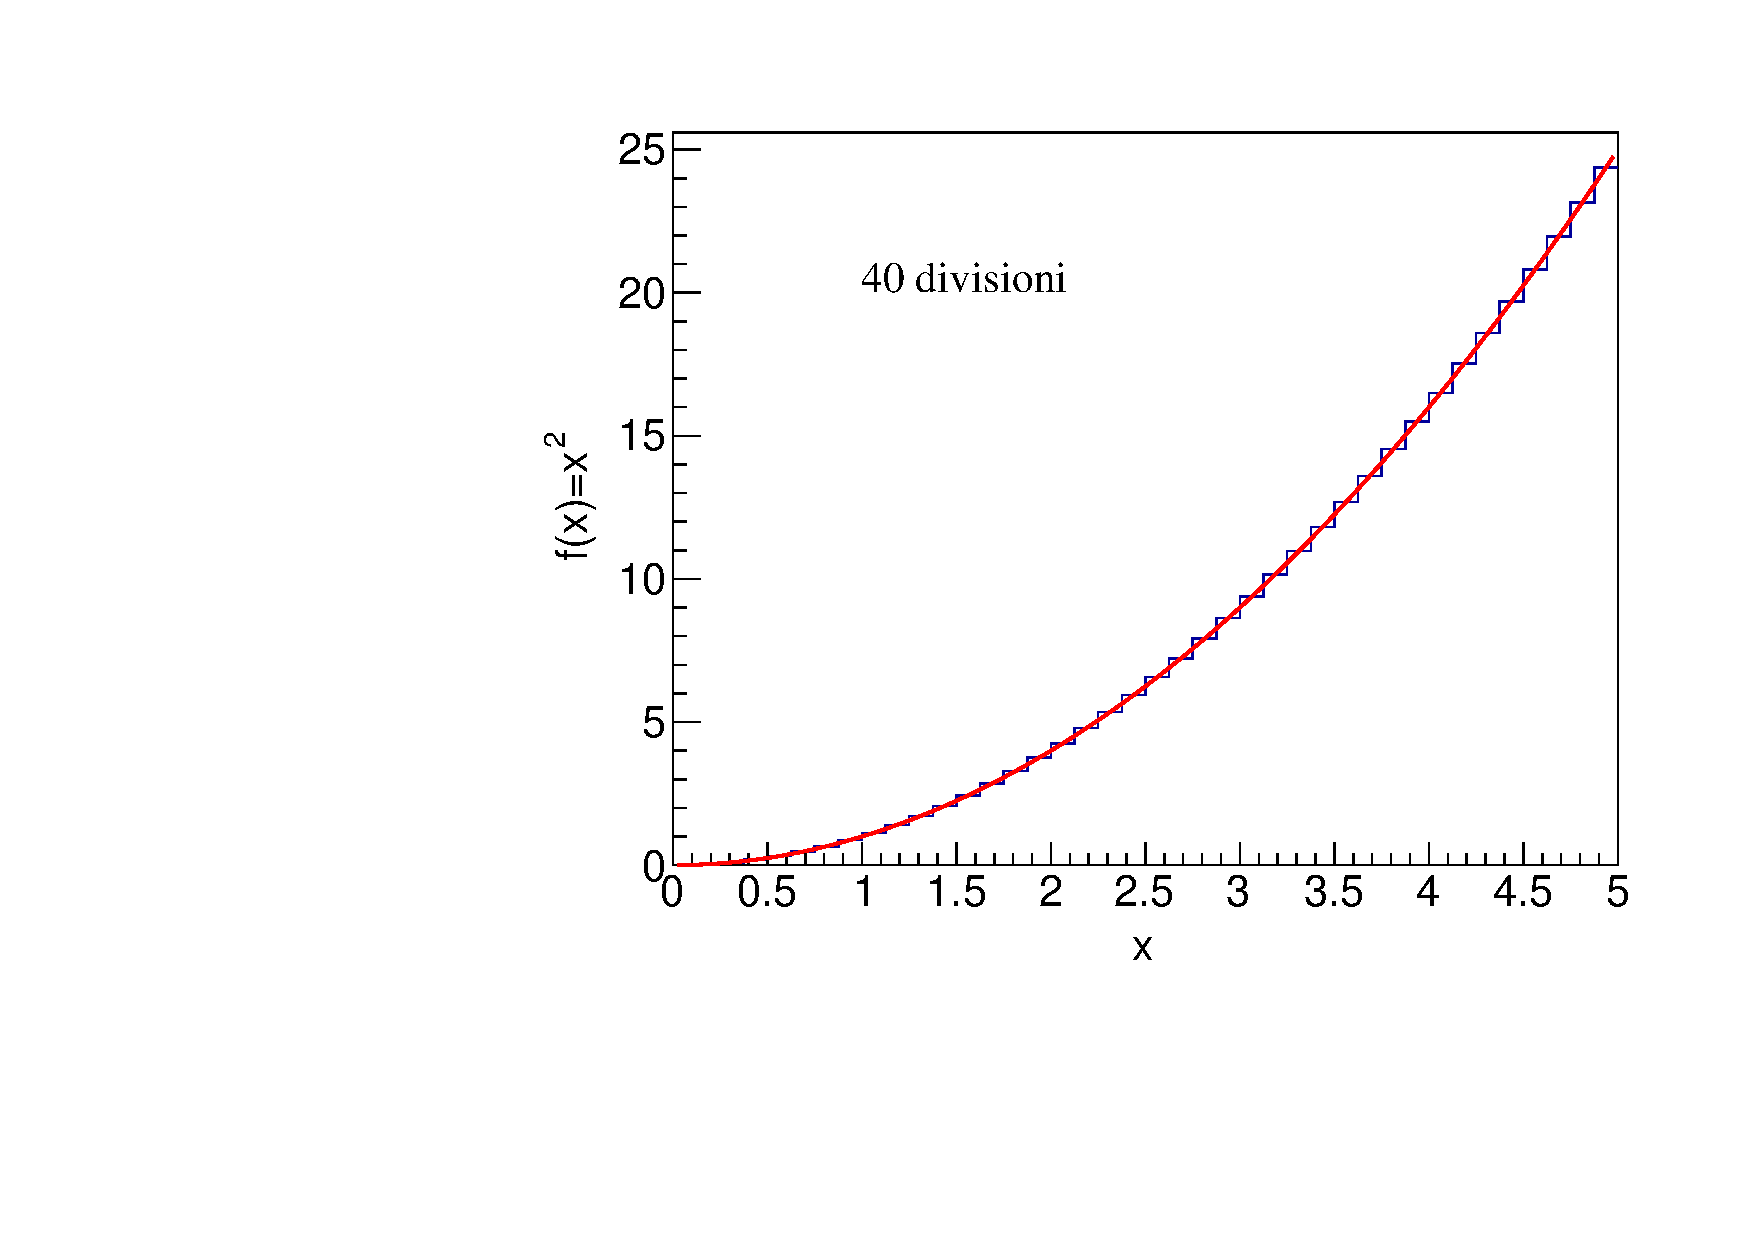
\includegraphics[scale=0.3]{./Pictures/intpar40.pdf}
\caption{Rappresentazione del metodo dei rettangoli per l'integrale della funzione $f(x)=x^2$ tra 0 e 5, utilizzando 10, 20, 30 e 40 divisioni. \label{rettangoli}}
\end{figure}



Sfruttiamo questo esempio per introdurre l'utilizzo di una nuova libreria. Quando abbiamo bisogno di utilizzare funzioni matematiche come seno, coseno, tangente etc o operazioni tipo l'elevamento a potenza abbiamo bisogno di caricare la libreria che ci abilita a poter utilizzare queste funzionalità del linguaggio di programmazione. La libreria matematica standard si chiama $cmath$, e nel nostro esempio ci avvaleremo della funzione $pow$ (diminutivo di power) per elevare alla seconda potenza una variabile. Il costrutto di $pow$ è il seguente:
\begin{verbatim}
y = pow(base, potenza);
\end{verbatim}

Notare che la potenza può essere anche un numero razionale, ciò ci consente di utilizzare questa funzione per definire le operazioni di radice a qualunque ordine: potenza =1/2 - radice quadrata; potenza = 1/3 radice cubica; potenza = 7/5 - radice quinta di potenza 7 etc.

NOTA: Le funzioni trigonometriche sin(var); cos(var); tan(var) etc vogliono come informazione l'angolo espresso in radianti, quindi se avete dati espressi in angolo bisogna prima convertirli in radianti dividendo l'angolo per 180$^\circ$ e moltiplicando per $\pi$-greco. 



Di seguito i codici implementati durante il corso da due allieve,
uno con una implementazione standard e uno con una scrittura sintetica del ciclo \textbf{for}:

\begin{lstlisting}[language=c++]
//integrale di x^2
#include <iostream>
using namespace std;
main (){
float a=0, b=5;
float x; //misura dell'intervallo
float m; //punto medio di ogni intervallo
float Area=0;
x=(b-a)/100;
m=a+x/2;
for(int i=0; i<100; i++){
Area=Area+(x*(m*m));
m=m+x;
}
cout<<Area<<endl;
return 0;}
\end{lstlisting}

Nel codice seguente è molto bella la implementazione del ciclo \textbf{for} proposta da una studentessa del corso, probabilmente un esperto di programmazione potrebbe obbiettare che un codice compatto e furbo potrebbe essere poco leggibile, ma nonostante l'obbiezione legittima ho voluto mostrare come esempio questa implementazione perché anche la creatività ha un suo valore e deve essere incoraggiata, anche se poi un collega che non riesce a capire cosa abbiamo scritto ci dedicherà una litania di benedizioni.

\begin{lstlisting}[language=c++]
#include <iostream>
#include <cmath>
using namespace std;
float somma=0;
float x=0;
float a=0;
float b=5;
float m;
int main() {
m=(b-a)/7527;
x=m/2;
for(x;x<=5;x=x+m){
  somma= somma+m*pow(x,2);
}
cout<<"L'integrale e'  "<<somma<<endl;
return 0;
}
\end{lstlisting}

\subsubsection{Ricerca dinamica del numero di divisioni}\index{Ricerca dinamica del numero di divisioni}

L'esercizio del calcolo dell'integrale di una funzione semplice e regolare come una parabola ci fornisce la possibilità di implementare un nuovo codice, molto divertente, che ha bisogno dell'implementazione di un ciclo $while$ per rispettare le specifiche del problema.

Il nuovo esercizio consiste nello scrivere un programma capace di stimare il numero minimo di divisioni dell'intervallo di integrazione per raggiungere un certo grado di precisione. La funzione in oggetto è molto semplice, ma anche fosse stata più complicata a patto di essere capaci di integrarla analiticamente, possiamo facilmente integrarla in modo esatto e a questo punto spostare l'oggetto del nostro desiderio dall'integrazione alla precisione dell'integrazione. 

\begin{lstlisting}[language=c++]
#include <iostream>
#include <cmath>
using namespace std;
int main (){
float a=0, b=5;
float j=1;
float x;
float m;
float Area=0;
while((fabs(125./3.-Area))>0.001){
  j++;
  x=(b-a)/j;
  m=a+(x/2.);
  Area=0;
  for(int i=0; i<j; i++){
    Area=Area+(x*m*m);
    m=m+x;
  }
}
cout<<"L'area e': "<<Area<<endl;
cout<<"Il numero di intervalli minimo e': "<<j<<endl;
return 0;
}
\end{lstlisting}

In questi due versioni dell'esercizio abbiamo visto come calcolare, con una algoritmo elementare, l'integrale di una funzione semplice. Più avanti, quando tratteremo le funzioni, riproporremo l'esercizio risolvendolo con una tecnica che non richiede la conoscenza a-priori del valore dell'integrale della funzione. 


\subsection{Bandiera crociata - uso combinato di cicli e strutture di controllo I}\index{Bandiera crociata - uso combinato di cicli e strutture di controllo I}

L'esercizio in questo paragrafo è asciutto e apparentemente arido, ma guardandolo bene ci consente di comprendere come funzionano i cicli e le condizioni logiche e come si costruisce un algoritmo:

\begin{verbatim}
Scrivere un codice capace di stampare a schermo il seguente schema numerico quadrato:
 1  0  0  0  0  0  0  0  0  0  1 
 0  1  0  0  0  0  0  0  0  1  0 
 0  0  1  0  0  0  0  0  1  0  0 
 0  0  0  1  0  0  0  1  0  0  0 
 0  0  0  0  1  0  1  0  0  0  0 
 0  0  0  0  0  1  0  0  0  0  0 
 0  0  0  0  1  0  1  0  0  0  0 
 0  0  0  1  0  0  0  1  0  0  0 
 0  0  1  0  0  0  0  0  1  0  0 
 0  1  0  0  0  0  0  0  0  1  0 
 1  0  0  0  0  0  0  0  0  0  1
 
Generalizzare il codice in modo da poter scegliere il numero di righe
o di colonne. Ovviamente nello schema il numero di righe e di colonne
resta sempre lo stesso.
\end{verbatim}

Il primo approccio per risolvere questo problema è quello di spegnere il computer, 
scrivere la tabella su un foglio di carta e pensare, e farlo fino a quando non si trova il metodo automatico per generare la sequenza che il problema ci propone di generare. 
La prima osservazione della tabella ci dice che tutti i numeri che stanno sulle diagonali del quadrato rappresentato dalla tabella valgono 1 mentre tutti gli altri valgono zero. Ma questo non è ancora sufficiente a risolvere il problema,
e quindi per fare questo, una possibile strategia potrebbe essere quella di immaginare un sistema per etichettare ogni posizione dei numeri, come ad esempio numerare le colonne e le righe della tabella e individuare ogni punto attraverso questi due numeri. Fatto questo abbiamo quasi finito, a questo punto risulta banale notare che tutti gli elementi su una diagonale possono essere definiti dalle condizioni che o il numero di riga e quello di colonna devono coincidere o che la somma del numero di riga e quello di colonna debbano essere pari al numero totale di riga (o di colonna, la tabella è quadrata).  Di seguito il codice:

\begin{lstlisting}[language=c++]
#include <iostream>
#include <fstream>

using namespace std;

int main(){
   int condiz;
   int dim =10; //dimensioni della tabella
   ofstream pippo("filematricioso.cuc"); //il nome del formato e' inventato
                                         77serve solo a rammentare che e' bene
                                         // mettere l'estensione
   do{
   for(int a=0; a<=dim;a++){  //a e' l'indice su riga
      for(int b=0; b<=dim; b++){//b indice di colonna
          if(a==b||a+b==dim){
            pippo<<" 1 ";
            }
          else{
            pippo<<" 0 ";
            }
        }
        pippo<<endl;  //seconda istruzione del for su a 
      }

     cout<<"vuoi stampare una nuova matrice?"<<endl;
     cout<<"Si, allora digita 1"<<endl;
     cin>>condiz;
     if(condiz==1){
     cout<<"mi dici la dimensione della matrice?"<<endl;
     cin>>dim;
     }
   }while(condiz==1);
   return 0;
}
\end{lstlisting} 

Nel codice appena implementato, facciamo un esempio dell'uso dei cicli \textbf{for} e \textbf{do-while}, del costrutto della struttura decisionale \textbf{if} e abbiamo
inoltre introdotto una doppia condizione nell'\textbf{if} concatenata con l'operatore \textbf{or} (\textbf{||}) per includere entrambe le diagonali.

\subsection{Risoluzione di un sistema di equazioni lineari con il metodo di Gauss - uso combinato di cicli e strutture di controllo II}\index{Bandiera crociata - uso combinato di cicli e strutture di controllo I}

Il codice presentato in questo paragrafo risolve il problema della ricerca delle soluzioni di un sistema lineare di 3 equazioni in 3 incognite con il metodo di Gauss. Il codice è facilmente generazzabile a sistemi di equazioni con un numero di incognite qualunque.
Il programma legge i dati da un file esterno e restituisce la soluzione del sistema.



\begin{lstlisting}[language=c++]
//Implementazione di un codice capace di risolvere un sistema lineare
//in tre incognite con il metodo della tringolarizzazione di Gauss

#include <iostream>
#include <fstream>

using namespace std;

int main(){
/* struttura degli indici dei termini noti del sistema
   (0,0)x + (0,1)y + (0,2)z = (0,3)
   (1,0)x + (1,1)y + (1,2)z = (1,3)
   (2,0)x + (2,1)y + (2,2)z = (2,3)

Lo scopo e' azzerare i coifficienti (1,0), (2,0), e (2,1)
e' faciele vedere come questi formino un triangolo sotto la 
diagonale della tabella dei coefficienti delle incognite.
L'azzeramento avviene attraverso operazioni lineari tra
le righe della tabella
*/

// Contenitore dei coefficienti
  int numrighe = 4;
//  int numcol   =5; 
  double coef[numrighe][numrighe+1]; //coefficienti 3 righe 4 colonne

  ifstream pippo("dati.dat"); //file che contiene i coefficienti del sistema
  cout<<"i coefficienti di un sistema 4 incognite sono"<<endl;
//lettura dei coefficienti del sistema!! 
  for(int i =0; i<numrighe; i++){
    for(int j=0; j<numrighe+1;j++){
      pippo>>coef[i][j];
    }
  }
//***************************!!

//stampa dei coefficienti del sistema!! 
  for(int i =0; i<numrighe; i++){
    for(int j=0; j<numrighe+1;j++){
      cout<<coef[i][j]<<"  ";
    }
    cout<<endl;
  }
  cout<<endl;
  cout<<endl;
//***************************!!

//variabili di servizio per il processo di triangolarizzazione!!
  double denom, numen,secchio;
  int xx=1;//serve per trovare la riga con cui fare lo scambio
//***************************!!


  for(int k =0; k<numrighe-1;k++){ //ciclo sulle colone da azzerare
    
    numen=coef[k][k];
// se questo coefficiente e' uguale a zero non ci consente di effettuare la triangolarizzazione
// quindi si procede a cercare una riga il cui primo elemento sia diverso da zero in modo
// da fare un semplice s
    if(numen==0){
//questo ciclo while cerca la prima riga utile per fare lo scambio
      while(coef[k+xx][k]==0){
	xx++;
      }
//il ciclo for effettua l'operazione di scambio delle righe
      for(int m =0; m<numrighe+1;m++){
	secchio = coef[k][m];
	coef[k][m]=coef[k+xx][m];
	coef[k+xx][m]=secchio;
      }
//si aggiorna il valore della variabile numen per gli usi successivi
      numen=coef[k][k];
//si reinizializza xx a 1 nel caso ci sia bisogno nuovamente di questa procedura di controllo
      xx=1; 
    }

    for(int i =k+1; i<numrighe; i++){
   // le colonne
      denom=coef[i][k];
      //condizione che protegge dagli zeri sul triangolo, se zero non faccio nulla e passo al prossimo
      if(denom!=0){ 
	for(int j=k; j<numrighe+1; j++){
	  coef[i][j] =  coef[k][j]- (coef[i][j]/denom)*numen;
	}//ciclo su j
      }//if proteggi sono gia' zero
    }//ciclo su i
  }//ciclo su k

  //stampo il risultato finale
  for(int i =0; i<numrighe; i++){
    for(int j=0; j<numrighe+1;j++){
      cout<<coef[i][j]<<"  ";
    }
    cout<<endl;
    
  }
  
double sol[numrighe];

for(int i=numrighe-1; i>-1;i--){
sol[i]=coef[i][numrighe];

for(int j=i;j<numrighe-1;j++){
sol[i]-= sol[j+1]*coef[i][j+1];
}

sol[i]= sol[i]/coef[i][i];

}

for(int i =0; i<numrighe;i++){
cout<<"soluzione "<<i+1<<" = "<<sol[i]<<endl;
}


  return 0;
}
\end{lstlisting}




\section{ifstream e ofstream: lettura e scrittura su file}\index{ifstream e ofstream: lettura e scrittura su file}

Per leggere e scrivere su file il c++ fornisce due strumenti 
appartenenti alla librerie fstream\footnote{NOTA BENE: ci dobbiamo 
ricordare di mettere in testa la scrittura 	\#include $<$fstream$>$ 
altrimenti non possiamo usare questi strumenti.} che si chiamano 
\textbf{ifstream} e \textbf{ofstream}. \'E facile memorizzare che \textbf{ifstream} serve per
leggere, infatti la i sta per input e la f per file, mentre \textbf{ofstream} 
serve per scrivere su file, la o ovviamente sta per output.

Mostriamo di seguito il costrutto dei due operatori, prima iniziamo dall'operatore di lettura:

\begin{verbatim}
ifstream leggimi;
leggimi.open("nomedelfiledilettura.dat"); 
float dato;
leggimi>>dato;
cout<<"ecco cosa abbiamo letto: "<<dato<<endl;
leggimi.close();
\end{verbatim} 

Poi mostriamo quello dell'operatore di scrittura:


\begin{verbatim}
ofstream scrivimi;
scrivimi.open("nomedelfilediscrittura.dat"); 
for(int i=0;i<100;i++){
   scrivimi<< i <<endl;
}
scrivimi.close();
\end{verbatim}

Osservando i due costrutti possiamo notare che i due operatori differiscono per il nome e la loro funzione, ma il loro utilizzo è molto molto simile. Infatti la sintassi di apertura e chiusura del file\footnote{Nota bene: Chiudere il file è importantissimo. Lasciare un file aperto significa dare accesso al sistema operativo alle locazioni di memoria riservate al documento con la possibilità che questo possa essere danneggiato.} è la stessa mentre l'operatività degli operatori è identica a quella delle operazioni di input-output da/su terminale \textbf{cin} e \textbf{cout} attraverso gli operatori $>>$ e $<<$.


Ogni operazione di lettura o di scrittura muove il punto di lettura al successivo valore che deve essere letto o scritto: in altre parole il computer legge o scrive in maniera progressiva nel file. Per ``riavvolgere il nastro'' ovvero per spostare il punto di lettura/scrittura ci sono apposite funzionalità (\textbf{seekg}, \textbf{seekp}). 

Le classi \textbf{ifstream} e \textbf{ofstream} hanno diverse funzionalità alle quali si accede attraverso l'operatore . (si proprio così l'operatore punto). Abbiamo visto in azione già l'operazione di apertura e chiusura del file, e negli esempi che seguono vedremo le operazioni \textbf{eof()} che ci dice se si è arrivati alla fine del file o meno, le funzioni \textbf{clear()}, \textbf{seekg} e \textbf{seekp} che servono per spostare il punto di lettura o scrittura del file (li useremo per riportare il punto di lettura all'inizio del file dopo aver effettuato una prima lettura).

\subsection{Lettura di un file di un numero incognito di quantità}\index{Lettura di un file di un numero incognito di quantità}

Una operazione molto utile è quella di essere capaci di leggere un file di dati il cui numero ci è incognito. A questo punto potremmo fare l'obiezione che è difficile immaginare una simile evenienza. In realtà non è così. Immaginiamo di avere il compito di analizzare dati che provengono da una stazione di monitoraggio di quantità fisiche, per esempio una stazione che monitora la temperatura, o la pressione o la radioattività o etc e che salva queste letture su un file di testo e che effettua una lettura ogni certa quantità di tempo.
In un certo momento della giornata scarichiamo il file contenete questi dati e iniziamo ad analizzarli.

Il numero di dati contenuti non ci è noto, e noi non abbiamo il tempo e il modo di aprire il documento e di contare il numero di dati che il file contiene. La soluzione è scrivere un programma capace di farlo in maniera automatica, di fornirci il numero di dati che abbiamo letto, e quindi procedere con delle semplici analisi.

\subsubsection{lettura del X-file}

Per risolvere questo problema faremo uso di un ciclo \textbf{while} che ci consente di implementare un ciclo con numero di ripetizioni variabili e dipendenti dalla condizione che lo governa e la funzione \textbf{eof()}\footnote{eof sta per end of file.} dell'operazione \textbf{ifstream} che ci dice se ci troviamo alla fine del file oppure no. L'operazione \textbf{eof()} risponde in modo diretto alla domanda, nel senso che restituisce 1 (vero) se è arrivato alla fine e 0 (zero)  in caso contrario. Per usare questo comportamento come condizione per governare il ciclo \textbf{while} dobbiamo usare l'operatore punto esclamativo (!) per negare la risposta della funzione \textbf{eof()} in maniera tale che quando lui ci dice che non è alla fine noi diciamo al \textbf{while} di effettuare un'altra lettura e quando invece ci dice che è arrivato alla fine noi diciamo al \textbf{while} di uscire dal ciclo.

Riportiamo di seguito il frammento di codice per la lettura del file e il conteggio del numero di letture:

\begin{verbatim}
ifstream leggimi;
leggimi.open("Xfile.dat");
double temperatura;
int NumerodiConteggi=0;
while (!leggimi.eof()){
  leggimi>>temperatura;
  if (!leggimi.eof()) {
     cout<< temperatura << endl;
     NumerodiConteggi++;
  }
}
cout<< il numero di conteggi è <<NumerodiConteggi<<endl;
\end{verbatim}

 Commentiamo brevemente il codice che abbiamo scritto: prima di tutto abbiamo creato l'operatore di lettura, aperto il file e creato le variabili su cui copiare la singola lettura e su cui effettuare un conteggio (inizializzata a 0); dopo di che il ciclo \textbf{while} verifica se la sua condizione che la governa è vera oppure no. Se è vera c'è almeno un dato dentro il file. A questo punto entriamo dentro il ciclo e procediamo  a leggerlo procedura per procedura: leggiamo un valore e lo copiamo nella variabile temporanea "temperatura", controlliamo sull'\textbf{if} se è vero che abbiamo letto un valore, lo stampiamo a monitor e poi incrementiamo il contatore, ripassiamo la palla al \textbf{while} e così via.
 Quando processo legge l'ultimo dato valido del file continuerà a soddisfare la condizione del \textbf{while} entrerà nel ciclo ed effettuerà una lettura che fallirà perché non c'è un altro dato da leggere, la condizione \textbf{if} non consentirà di stampare nulla a schermo ne di incrementare il contatore, dopo di che si esce definitivamente dal \textbf{while} e si stampa a monitor il valore esatto del numero dei lettura.
 
 Il processo di lettura non interpreta gli spazi vuoti o gli "a capo" e non fa differenza tra file in cui i dati sono scritti in modo ordinato o disordinato, il processo legge elemento ad elemento.
 Se un file è ordinato e lo vogliamo leggere noi sfruttando questa informazione è nostra responsabilità adottare una strategia capace di utilizzarla al meglio.
 
 Esempio se i dati sono ordinati su due colonne dove sulla prima colonna mettiamo una quantità fisiche indipendente e sulla seconda una quantità dipendente dalla prima basta scrivere un codice in questo modo:

\begin{verbatim}
ifstream leggimi;
leggimi.open("Xfile.dat");
double temperatura, Energia;
while (!leggimi.eof()){
  leggimi>>temperatura>>Energia;
  if (!leggimi.eof()) {
     cout<< temperatura << "  "<< Energia<< endl;
  }
}
\end{verbatim} 

Visto che siamo capaci di accedere ai dati e di stamparli a monitor, possiamo avventurarci nello studio degli stessi e provare a calcolare la media e lo scarto quadratico medio utilizzando le seguenti formule 
$$<T> = \sum_{i=0}^N \frac{t_i}{N}$$ 
$$\sigma = \sqrt{\sum_{i=0}^N \frac{(<T>-t_i)^2}{N}}$$
e con il seguente codice

\begin{lstlisting}[language=c++]
//calcola la somma e la media

ifstream leggimi(nome);   //legge dal file dati.dat
double a;   //variabile di copia provvisoria
double somma =0;  //accumulatore
int NumerodiLetture = 0; //contatore         
while(!leggimi.eof()){
  leggimi>>a;   //attribuisce i valori del file alla variabile a, 
                //finche' non siamo arrivati alla fine del file
  somma=somma+a;
  if(!leggimi.eof()){
    cout<<a<<endl;      //stampa i valori del file
    NumerodiLetture++;
  }
}
media=somma/NumerodiLetture;   //calcola la media
cout<<endl;
cout<<"Hai stampato "<<NumerodiLetture<<" numeri."<<endl;
cout<<"La somma dei numeri stampati e' "<<somma<<".\n";
cout<<"La media dei numeri stampati e' "<<media<<" \n";
leggimi.close();  //chiusura del file
\end{lstlisting}


\subsubsection{Scorciatoria nel processo di lettura}

Nel paragrafo precedente abbiamo fatto vedere come servirsi del metodo eof() (end of file) combinato
con il ciclo while per leggere tutti i dati contenuti in un file. Un trucco molto utile che si può usare
per semplificare il codice di lettura è quello di sfruttare la proprietà della procedura di lettura attreverso un oggetto di tipo ifstream che restitutisce il valore 1 (vero) se è stato capace di effettuare la lettura eil valore 0 (falso) in caso contrario. In altre parole il seguente codice:

\begin{verbatim}
ifstream leggimi("dati.dat");
double dato;
while{leggimi>>dato){
cout<<dato<<endl;
}
\end{verbatim} 
è capace di stampare a schermo tutti i dati contenuti nel file dati.dat.


\subsubsection{Dimenticavo...se smarrite il file di lettura, che succede?}

Nel caso in cui indicaste al vostro oggetto di tipo ifstream un file da leggere, che per qualunque ragione non sia
raggiungibile, nel senso che il file da leggere non esiste, esiste ma è errato il percorso di lettura, avete sbagliato a scrivere il nome... che cosa succede al vostro codice?
 
\subsection{Caricare dati in un vettore e ricerca dei max e min assoluti}\index{Caricare dati in un vettore e ricerca dei max e min assoluti}

Nella sessione precedente abbiamo imparato a leggere un file con un numero di dati incogniti e a farci dire il numero di letture.
Ora scriveremo un codice capace di caricare i dati in un vettore di dimensione pari al numero di letture e di trovare il massimo assoluto e il minimo assoluto tra i valori letti.

Per creare un vettore delle dimensioni giuste, capace di contenere i nostri dati, prima di tutto dobbiamo conoscere quanto è questa dimensione e per avere questa informazione ci sono diverse opzioni: la conosciamo (evviva, fine); apriamo il file e li contiamo (che noia!!!!!); le contiamo con il nostro codice (che forti che siamo!!!). La conoscenza di questo numero è importante perché se imponiamo una dimensione inferiore a quella necessaria il programma di lettura cercherà di scrivere i dati in allocazioni di memoria non riservate al vettore e otterremo un errore nella esecuzione del programma (NOTA BENE - non in fase di compilazione ma in fase di esecuzione) se invece mettiamo prudentemente un numero enorme probabilmente potremmo essere al sicuro da questo problema (ma non è detto) ma violeremmo il principio di richiesta minima di risorse (in questo caso memoria) che è sempre importante tenere presente, anche nell'epoca dei Giga- e dei Tera-Byte. 

Quindi prima contiamo e creiamo il vettore e poi...??? A questo punto dobbiamo riavvolgere il nastro. Si esatto l'oggetto che abbiamo usato per leggere è arrivato alla fine del file e quindi non può più accedere ai dati. Bisogna dirgli di ricominciare da capo. Questo lo possiamo fare o con un trucco, cioè chiudiamo e riapriamo il file
\begin{verbatim}
leggimi.close();    //chiude il file
leggimi.open("dati.dat"); // la riapertura del file mette il "cursore"
                          // dell'ifstream all'inizio del file
\end{verbatim}
oppure possiamo usare i metodi offerti dalla classe ifstream come segue
\begin{verbatim}
leggimi.clear(); //resetta le etichette di errore, 
                 //è necessaria prima di una operazione di rewind
leggimi.seekg(0); //rimettiamo il riferimento del sistema 
                  //di lettura al primo elemento, realizza il rewind

\end{verbatim}

Ora siamo finalmente pronti per caricare i nostri dati in un vettore delle dimensioni giuste.

\begin{verbatim}
float misure[NumerodiLetture];//crea il vettore che fa per noi!
for(int i=0; i<NumerodiLetture; i++){                     
   leggimi>>misure[i];
}
leggimi.close(); chiudiamo definitivamente!
\end{verbatim}

I dati sono caricati in una variabile ed è a nostra completa disposizione, e quindi possiamo per esempio trovare quale sia il massimo e il minimo assoluto tra i dati che abbiamo letto:


\begin{verbatim}
//restituisce il valore massimo e il valore minimo

float max, min;
max=misure[0]; //inizializziamo al primo valore
min=misure[0];
for(i=0; i<NumerodiLetture; i++){
  if(misure[i]>max){
    max=misure[i];}
  else if(misure[i]<min){
  min=misure[i];}
}
cout<<"Il valore minimo e': "<<min<<endl;
cout<<"Il valore massimo e': "<<max<<endl;
\end{verbatim}

Questo esercizio oltre a contribuire a renderci più familiare la scrittura di un codice, fornisce un pezzo di programma fondamentale per la costruzione di un istogramma.



\subsection{Costruzione di un istogramma}\index{Costruzione di un istogramma}
\label{istocostr}

Prima di iniziare a scrivere un programma per la risoluzione di un problema bisogna conoscere e capire bene il problema. Non avere nessun dubbio su ciò che ci serve e su cosa bisogna fare.

Quindi prima di tutto proviamo a capire che cosa sia un istogramma.
Un istogramma è un modo ``ordinato'' di rappresentare i dati/misure ripetute di una stessa quantità (istogramma monodimensionale) o di più quantità in relazione tra di loro (istogramma multidimensionale) che ci consente di leggere in modo veloce le informazioni statistiche contenute nei dati.

Un modo di costruire un istogramma potrebbe essere quello di individuare il massimo e il minimo assoluto dell'insieme di dati che si vogliono usare per costruire l'istogramma; usare questi due valori per determinare l'intervallo di variabilità dell'istogramma; poi si divide l'intervallo di variabilità in un numero arbitrario di sotto-intervalli (di uguale ampiezza nel nostro esempio, ma esistono anche rappresentazioni con intervalli di ampiezza variabile), i sotto intervalli vengono chiamati in gergo ``bin''\footnote{bin in inglese vuol dire secchio, parola azzeccata e figurativa in quanto i sotto intervalli di un istogramma si comportano esattamente come un contenitore nel quale uno accumula i dati come quando si mettono oggetti in un contenitore.}; infine bisogna contare per ogni sotto intervallo quante misure sono comprese nei rispettivi limiti del sotto intervallo stesso.
Se in ogni sotto intervallo registriamo il numero di volte che una misura cade nel sotto intervallo, l'istogramma si dice delle frequenze assolute, se invece questo numero è diviso per il numero del campione allora si dice che l'istogramma è delle frequenze relative.

Di seguito viene riportato il codice capace di assolvere questo compito. Il codice stampa a schermo su una colonna il valore medio di ogni sotto-intervallo e su una seconda colonna la frequenza assoluta delle misure nel sotto-intervallo.

\begin{lstlisting}[language=c++]
//creare istogramma
int rebinning=0;//entra comunque la prima volta
do{ //per ripetere il ciclo, e cambiare binnaggio
 int nint;  //nint=numero intervalli
 cout<<"\nInserisci il numero di intervalli dell'istogramma: \n";
 cin>>nint;
 float l=(max-min)/(float)nint;//larghezza intervalli          
 cout<<"larghezza intervalli: "<<l<<endl;
 int bin[nint]; //crea un vettore di dimensione pari a nint
 for(i=0;i<nint;i++){
	bin[i]=0; //inizializza a zero i valori di ogni intervallo
	}
 for(i=0;i<nint;i++){
   for(int v=0; v<j; v++){
    if((misure[v]>=min+i*l)&&(misure[v]<=min+(i+1)*l)){ 
//per ogni intervallo conta quali valori cadono entro l'intervallo stesso 
    bin[i]++;
    }
   }
  }
                                               
//incrementa il numero di valori per l'intervallo preso in considerazione
//cout << scientific;
 cout << fixed; //risolve il problema dell'allineamento
 cout<<"\nIstogramma:"<<endl;
 for(int n=0; n<nint; n++){                                         
  cout<<min+l/2+n*l<<"\t"<<bin[n]<<endl;                
 }
//stampa istogramma e valori medi di ogni intervallino
 cout<<"\n Numero diverso di intervalli? (Se si, premere 1):\n";
 cin>>rebinning;
 }while(rebinning==1);
\end{lstlisting} 

Analizzando un file creato appositamente con un codice MC, una distribuzione gaussiana, con questo codice otteniamo:

\begin{verbatim}
Inserisci il numero di intervalli dell'istogramma: 
15
Larghezza intervalli: 1.522647

Istogramma:
-4.049477	21
-2.526830	154
-1.004183	1038
0.518463	4618
2.041110	13894
3.563756	27787
5.086403	36796
6.609050	31854
8.131697	18555
9.654344	7240
11.176990	1821
12.699636	329
14.222283	40
15.744930	3
17.267576	0

Numero diverso di intervalli? (Se si, premere 1):
0
gmandaglio75@buccellato:>
\end{verbatim}

Questa che vediamo è una rappresentazione numerica, non grafica, ma come dicevamo prima la tabella riassume delle informazioni statiche, infatti anche a colpo d'occhio notiamo che la massima frequenza è tra  
5.086403 e 6.609050, quindi il valore medio della distribuzione sarà un numero compreso tra questi due valori. Infatti nel calcolo diretto del valore medio effettuato negli esempi precedenti è risultato essere pari a 5.35344.

\begin{figure}[t]
\centering
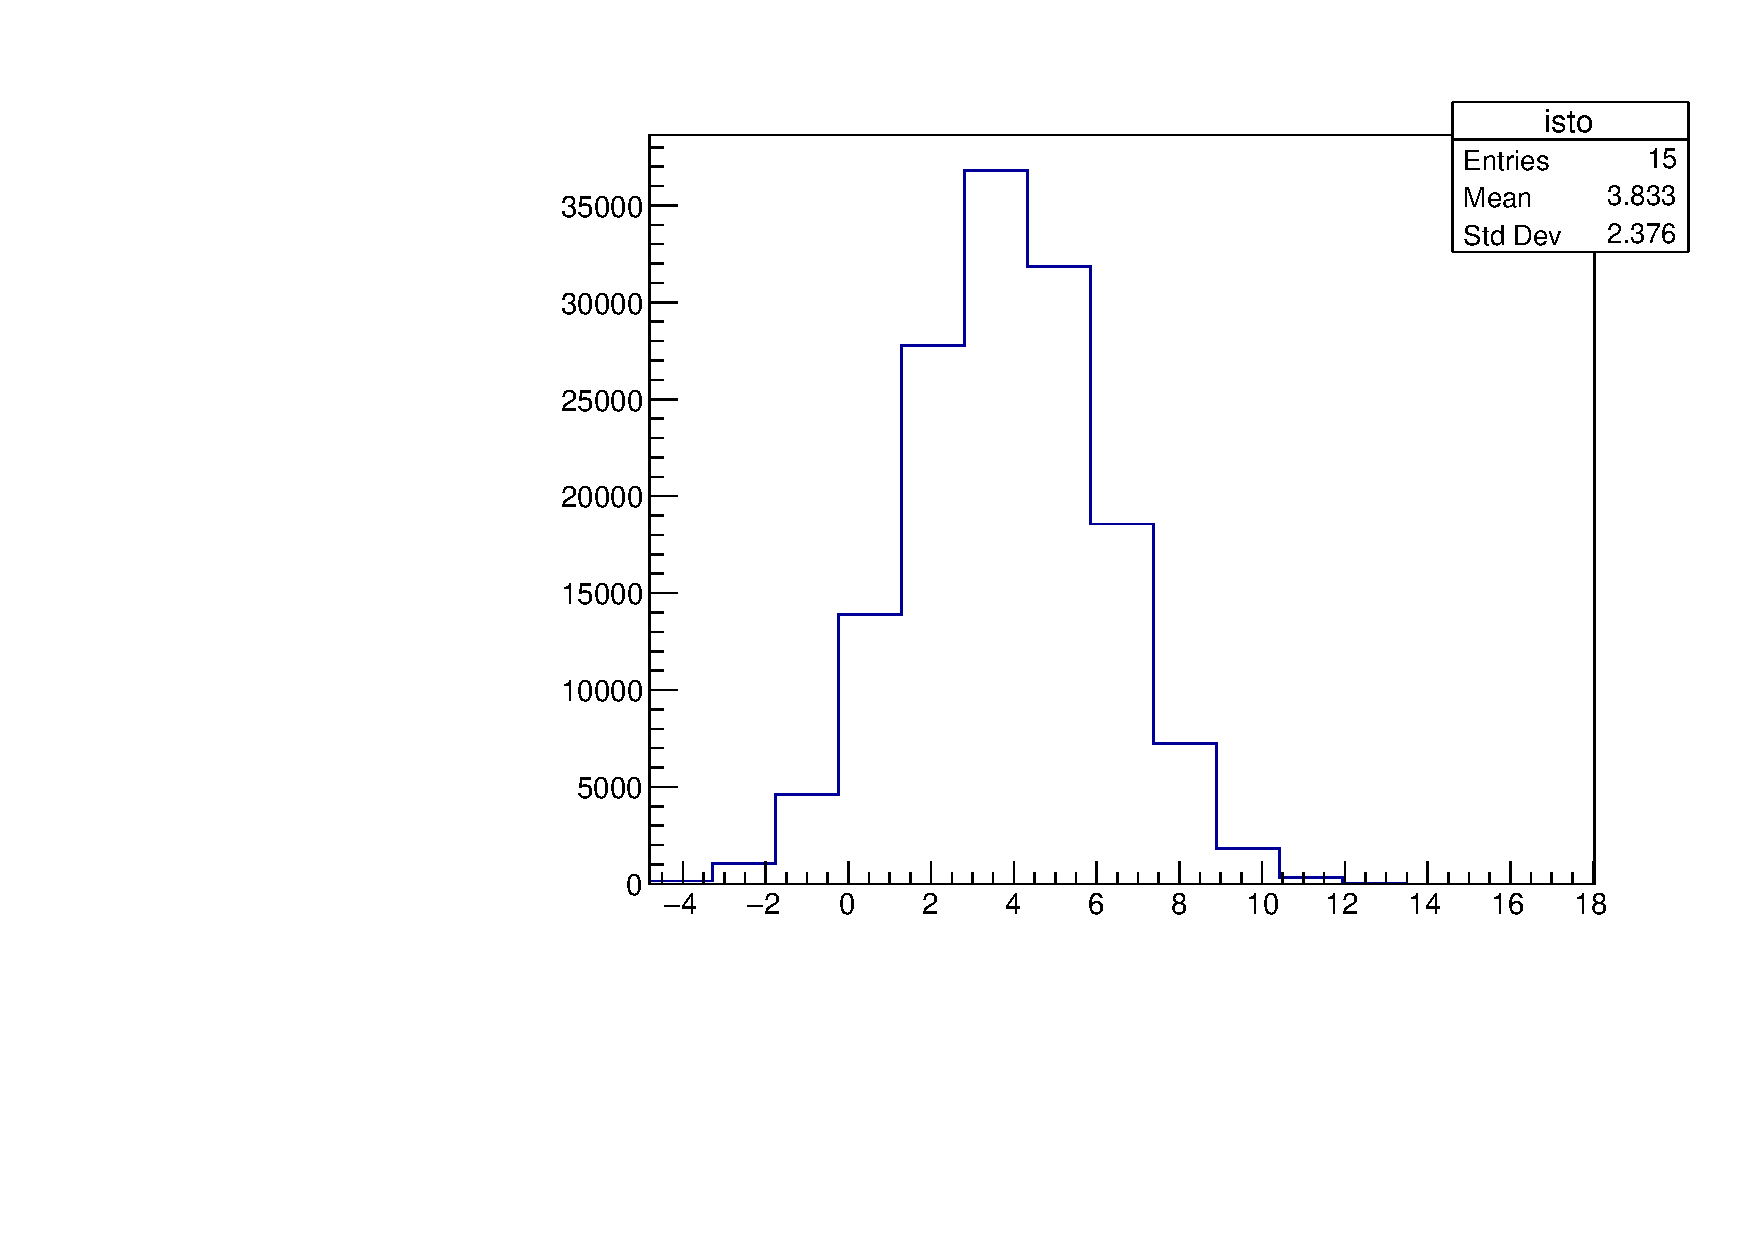
\includegraphics[scale=0.35]{isto.pdf}\\		
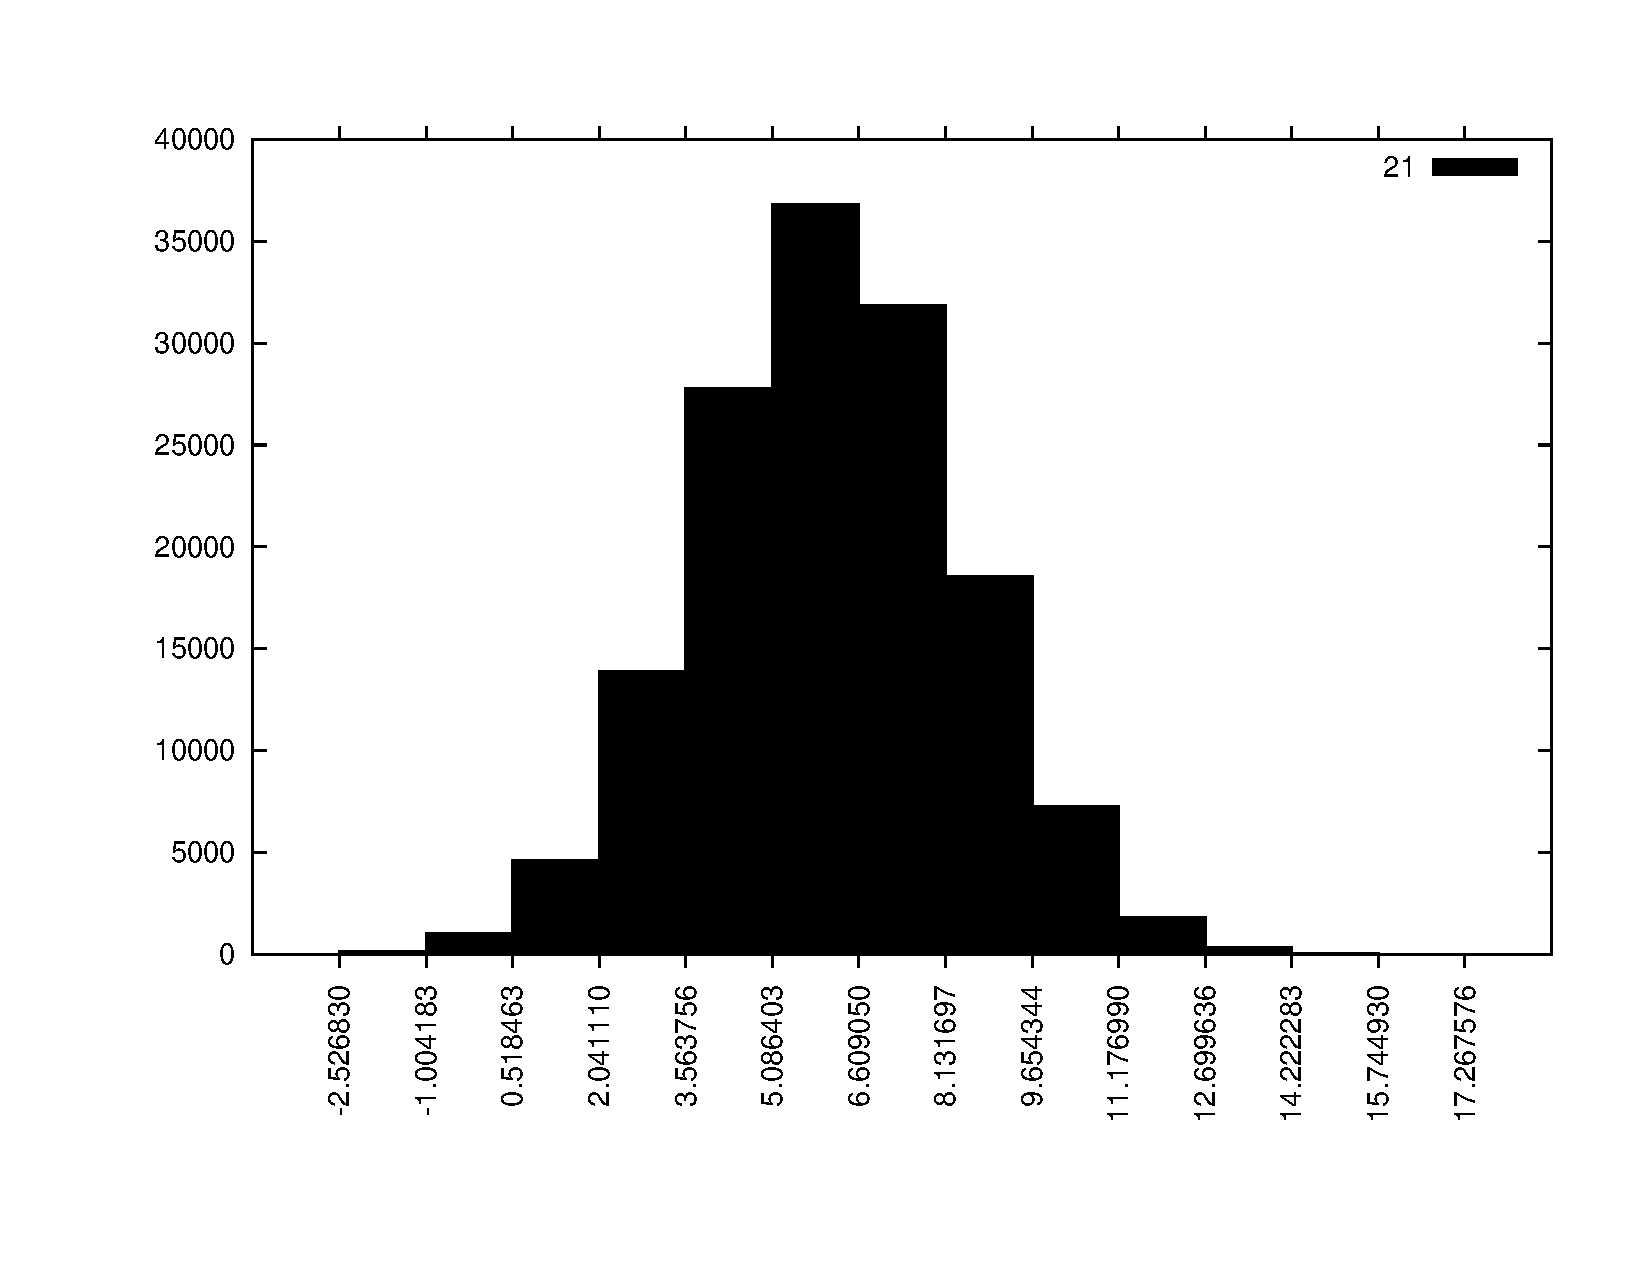
\includegraphics[scale=0.3]{printme.pdf}
\caption{Rappresentazioni dell'istogramma computato per 15 divisioni con root in alto e gnuplot in basso.\label{istos}}
\end{figure}

In figura \ref{istos} è rappresentato l'istogramma computato con il nostro codice per 15 bin con Root e gnuplot. Più avanti vedremo che le librerie di Root forniscono delle classi che ci consentono di costruire l'istogramma partendo dai dati grezzi. Il programma di grafica gnuplot ha bisogno che il lavoro di calcolo dell'istogramma sia fatto da noi. ROOT non è un programma di grafica ma un tool completo per l'analisi dati che possiede anche la capacità di fare grafica ad alto livello.


\section{Vettori e Matrici}

Sfruttiamo ciò che abbiamo imparato nella sezione precedente per fare un po' di pratica con i vettori e poi successivamente con le matrici.
Vettori e Matrici sono un comodo espediente per maneggiare con una sola variabile dati omogenei anche di grosse dimensioni.


\subsection{Vettore-semplice codice di ordinamento}

Sfruttiamo i codici che abbiamo implementato nella sezione precedente per leggere un file incognito, capire quante letture abbiamo fatto e quindi la dimensione da assegnare a un vettore, caricare i dati nel vettore, e poi implementare un semplicissimo algoritmo di ordinamento.

In questo semplice esercizio faremo pratica anche con la scrittura dei dati su file.

\begin{lstlisting}[language=c++]
#include <iostream>
#include <fstream>
#include <cmath>
using namespace std;

int main (){
  float pippo;

  ifstream leggimi("ordinami.dat");
  int numerodiletture=0;//contatore 
  while(!leggimi.eof()){//gli dico di leggermi il file
        leggimi>>pippo;
        if(!leggimi.eof()){
          numerodiletture++;
        }
  }
  leggimi.close();//lo chiudiamo

  leggimi.open("trovami.dat");
  double vettore[numerodiletture];
  for(int i=0; i<numerodiletture; i++)leggimi>>vettore[i];

  leggimi.close();

  ofstream scrivimi("ordinato.dat");
  
//*********BLOCCO CODICE CHE ORDINA*****************//  
  double min=10000000; //DEVE ESSERE UN REALE   
  int indicedelminimo =0;
  double bicchierevuoto;
  for(int partenza=0; partenza<(numerodiletture/3-1); partenza++){
    min=10000000;  //e' importantissimo mettere questa condizione
    for(int i=partenza; i<numerodiletture/3; i++){
      if(min>vettore[i]){min=vettore[i]; indicedelminimo=i;}
    }

    bicchierevuoto=vettore[indicedelminimo];
    vettore[indicedelminimo]=vettore[partenza];
    vettore[partenza]=bicchierevuoto;

    scrivimi<<vettore[partenza]<<endl;
  }
  
  
  scrivimi.close();
  return 0;
}
\end{lstlisting}


L'algoritmo di ordinamento cerca l'indice del vettore corrispondente al minimo assoluto dei valori contenuti nel vettore, scambia questo valore con quello del primo indice, il dato ordinato e ripete la procedura con i dati rimanenti ricorsivamente finché tutti i dati non sono ordinati.

Un esercizio giocoso da proporre a questo punto è chiedere quale sia il numero minimo di digitazioni per modificare il codice in modo che l'ordinamento non avvenga in ordine crescente ma in quello decrescente?\\
La risposta è 3. Ora però quali sono i tasti non ve lo dico :P .




\subsection{Matrice - ordinamento}

Ora immaginiamo di avere un file che contiene dati ordinati e distribuiti su 3 colonne e una certa quantità di righe. E che questi dati siano stati ordinati con delle proprietà che conosciamo, ad esempio le colonne contengono dati dello stesso tipo solo se appartengono alla stessa colonna mentre se guardiamo i dati rispetto alle righe questi sono tutti di natura differente ma sono accomunati dal fatto che sono stati misurati-creati nello stesso istante. Un esempio potrebbe essere dato da un sistema di rivelazione composto da tre sensori che misurano quantità fisica di diversa natura e un sistema di acquisizione che scrive su un documento le loro misure contemporanee al variare del tempo.

Come possiamo caricare queste informazioni in variabili che possono essere utilizzate da un codice?

\begin{lstlisting}[language=c++]
#include <iostream>
#include <fstream>
#include <cmath>
using namespace std;

int main (){
float trovami;
ifstream leggimi("trovami.dat");
int numerodiletture=0;//quanto e' lunga la colonna
while(!leggimi.eof()){//gli dico di leggermi il file (trovami)
        leggimi>>trovami;
        if(!leggimi.eof()){
                numerodiletture++;
        }
}
leggimi.close();//lo chiudiamo
leggimi.open("trovami.dat");
//creiamo la matrice [indice di riga][indice di colonna] 
double tabellina [numerodiletture/3][3];
for(int i=0; i<numerodiletture/3; i++){//numerodiletture=righe
  for(int j=0; j<3; j++){ //3 colonne
    leggimi>>tabellina[i][j];
  }
}
leggimi.close();
double min=10000000; //DEVE ESSERE UN REALE 
int indicedelminimo =0;

double bicchierevuoto;

for(int partenza=0; partenza<(numerodiletture/3-1); partenza++){
    min=10000000;  //e' importantissimo mettere questa condizione
  for(int i=partenza; i<numerodiletture/3; i++){
  if(min>tabellina[i][0]){min=tabellina[i][0]; indicedelminimo=i;}
}

for(int k=0; k<3;k++){
bicchierevuoto=tabellina[indicedelminimo][k];
tabellina[indicedelminimo][k]=tabellina[partenza][k];
tabellina[partenza][k]=bicchierevuoto;
}

cout<<tabellina[partenza][0]<<"  ";
cout<<tabellina[partenza][1]<<"  ";
cout<<tabellina[partenza][2]<<endl;
}
return 0;
}
\end{lstlisting}

Il codice che abbiamo appena scritto legge i dati da un file in cui ci sono tre colonne di dati e ordina i dati rispetto alla prima colonna con ordinamento crescente. Se volessimo ordinare rispetto alla seconda colonna basterebbe cambiare il secondo indice della matrice nella parte di codice di ricerca degli indici rispetto ai quali fare lo scambio:
\begin{verbatim}
for(int partenza=0; partenza<(numerodiletture/3-1); partenza++){
    min=10000000;  //è importantissimo mettere questa condizione
  for(int i=partenza; i<numerodiletture/3; i++){
  //cambiamo colonna
  if(min>tabellina[i][1]){min=tabellina[i][1]; indicedelminimo=i;}
}
\end{verbatim}
così come abbiamo appena fatto.

\subsubsection{Allocazione dinamica della memoria - malloc e new}

Sfruttiamo l'esempio precedente per spiegare l'allocazione dinamica della memoria. Un variabile array non è altro che una variabile di tipo puntatore, ovvero una variabile capace di memorizzare un indirizzo di memoria relativo ad uno spazio di memoria consecutivo capace di memorizzare un numero di dati, tutti dello stesso tipo, pari alle dimensioni dell'array.
Un array può essere utilizzato con la comoda notazione con le parentesi quadre che racchiudono gli indici oppure con l'algebra dei puntatori, 
\begin{verbatim}
//le due scritture sono equivalenti
cout<<vettor[3]<<endl;
cout<<*(vettore+2)<<endl;//+2 perchè si conta da zero
\end{verbatim}


E' bene ricordare che se si definisce un array non attraverso l'uso diretto dei puntatori, gli indirizzi che vengono memorizzati nelle variabili puntatori sono statiche, fisse e non possono essere modificate.

L'accesso alla memoria è una possibile sorgente di errori ma è anche una possibilità molto potente. Proviamo a dimostrarlo con un semplice esempio utilizzando il codice che abbiamo appena implementato per l'ordinamento.

Il seguente frammento di codice, una volta individuati gli indici per lo scambio, esegue ordinatamente lo scambio colonna per colonna:

\begin{verbatim}
for(int k=0; k<3;k++){
bicchierevuoto=tabellina[indicedelminimo][k];
tabellina[indicedelminimo][k]=tabellina[partenza][k];
tabellina[partenza][k]=bicchierevuoto;
}

cout<<tabellina[partenza][0]<<"  ";
cout<<tabellina[partenza][1]<<"  ";
cout<<tabellina[partenza][2]<<endl;
}
\end{verbatim}

e se le colonne del nostro documento fossero 10 al posto di 3, o 100, o 1000 etc? Mi direte, che problema c'è, cambiamo la condizione di stop del ciclo \textbf{for} e il gioco è fatto :)...e io mi seccherò come una biscia! In realtà la risposta è corretta, ma costringeremo il pc a eseguire 3 operazione per enne numero delle colonne. Grazie all'uso dei puntatori e della costruzione di una tabella (matrice) con l'allocazione dinamica della memoria potremo agilmente eseguire l'ordinamento effettuando solo le classiche tre operazioni di scambio. Lo scambio avverrà tra gli indirizzi di memoria che puntano alle locazioni di memoria in cui sono iscritti i dati di una intera riga (lunga quanto gli pare..).


Un matrice è costruibile con i puntatori utilizzando un puntatore doppio ($double **puntatoredoppio;$).
Un puntatore doppio è una variabile che contiene un indirizzo di memoria che si riferisce ad una zona di memoria riservata alla memorizzazione di indirizzi. Se in questa zona di memoria si memorizzano indirizzi che puntano a zone di memoria dove si possono memorizzare numeri, il gioco è fatto abbiamo creato una variabile capace di gestire una matrice.

Ora vederemo le implementazioni di una matrice con l'allocazione dinamica della memoria fatta con la funzione \textbf{malloc} di C o con l'operatore new (l'algebra dell'operatore new è mostrata nell'esempio che segue) di C++, ovviamente ciò che vale in C vale anche in C++ il contrario non è generalmente vero.

Implemantazione C-Style:
\begin{verbatim}
//libreria necessaria per usare malloc
#include <stdlib.h>
...
....

//ha bisogno della libreria stdlib.h compatibile con C
double** tabellina=  (double**)malloc((numerodiletture/3)*sizeof(double*));
for(int i = 0; i < numerodiletture/3; ++i)
    tabellina[i] = (double*)malloc(3*sizeof(double));

\end{verbatim}

Implemantazione C++-Style:

\begin{verbatim}
//libreria necessaria per usare malloc
#include <stdlib.h>
...
....
double** tabellina = new double*[numerodiletture/3];
for(int i = 0; i < numerodiletture/3; ++i)
    tabellina[i] = new double[3];
//scrittura equivalente, forse meno comoda
//  *(tabellina+i)= new double[3];
\end{verbatim}


A questo punto abbiamo la nostra matrice dinamica, e abbiamo accesso alle variabili indirizzo che la governano. Per effettuare l'ordinamento basterà scrivere:

\begin{verbatim}
//lavoriamo direttamente con gli indirizzi!!!
bicchierevuoto= tabellina[indicedelminimo];
tabellina[indicedelminimo]=tabellina[partenza];
tabellina[partenza]=bicchierevuoto;
\end{verbatim}

In un certo senso abbiamo reso una struttura bidimensionale in una monodimensionale.

\subsubsection{Ricerca binaria}
Una conseguenza dell'ordinamento di una sequenza di dati è la possibilità di fare delle ricerche degli indici della matrice in cui dati valori sono memorizzati. L'algoritmo più veloce è l'algoritmo di ricerca binaria o dicotomica.

Nell'esempio che segue presentiamo il frammento di codice che consente di trovare l'indice in cui è memorizzato il valore più prossimo a quello desiderato:

\begin{verbatim}
double valore=2.35;
int indice_alto=numerodiletture/3 -1; //indice più alto 
int indice_basso=0;			         //indice più basso 
int cont =0; //contatore: contiamo il numero di prove
int indicemedio=(indice_alto-indice_basso)/2;
//ciclo che realizza la ricerca binaria
while(fabs(tabellina[indicemedio][0]-valore)>0.5){			
  cont++;		
  if (tabellina[indicemedio][0] > valore){
    indice_alto=indicemedio;
  }
  else {
    indice_basso=indicemedio;       
  }
indicemedio=(indice_alto-indice_basso)/2;
}
\end{verbatim}


\section{Funzioni}\index{Funzioni}

In c/c++ qualunque programma e sotto-programma sono funzioni. Anche il programma principale è una funzione e si chiama \textbf{main} (in inglese vuole dire principale). Tutte le funzioni, compresa la principale, hanno lo stesso paradigma: cosa restituisce - nome della funzione - tra parentesi tonde ciò che riceve in input - l'implementazione della funzione segue racchiusa tra graffe.

Il codice che segue è la semplice implementazione di una funzione che  restituisce la somma di due numeri interi forniti alla funzione.
\begin{verbatim}
int somma(int a, int b){
return a+b;
}
\end{verbatim}

Ora però vediamo come le funzioni vengono implementati all'interno di un programma, come vengono chiamate e che regole devono essere eseguite.
Una regola che non ammette eccezioni è che ogni funzione, come del resto le variabili, deve essere dichiarata prima dell'esecuzione della funzione main. La dichiarazione della funzione si chiama prototipo. Il prototipo ripeto deve essere sempre dichiarato, la dichiarazione può coincidere con l'implementazione oppure no.
Le variabili che vengono usate per l'implementazione delle funzioni sono puramente simboliche, e in generale nella funzione principale non siamo tenuti a usare le stesse variabili.
Le variabili dichiarate all'interno di una funzione sono variabili locali.

Esempio prototipo e implementazione prima della funzione principale:
\begin{verbatim}
#include <iostream>
using namespace std;

int somma(int a, int b){
return a+b;
}
int main(){
int pino,pina;
pino =10;
pina=20;
cout<<somma(pino,pina)<<endl;
return 1;
}
\end{verbatim}



Esempio prototipo prima della funzione principale e implementazione dopo la funzione principale:
\begin{verbatim}
#include <iostream>
using namespace std;

int somma(int a, int b);

int main(){
int pino,pina;
pino =10;
pina=20;
cout<<somma(pino,pina)<<endl;
return 1;
}
int somma(int a, int b){
return a+b;
}
\end{verbatim}

Esempio in cui la funzione accessoria somma è stata scritta in un file "header" somma.h:

\begin{verbatim}
#include <iostream>
#include "somma.h"
using namespace std;
int main(){
int pino,pina;
pino =10;
pina=20;
cout<<somma(pino,pina)<<endl;
return 1;
}
\end{verbatim}

L'header file somma.h che in questo esempio vive nella stessa cartella che contiene il programma che lo carica attraverso la chiamata \#include contiene prototipo e implementazione della funzione:

\begin{verbatim}
// file somma.h
int somma(int a, int b){
return a+b;
}
\end{verbatim}



\subsection{Passaggio di valori a funzioni via value o reference}\index{Passaggio di valori a funzioni \textit{via value} o \textit{reference}}

Negli esempi del paragrafo precedente, senza dirlo abbiamo sempre usato il metodo di passaggio di valori alla funzione per valore (in inglese \textit{via value}). Passare delle variabili utilizzati in una funzione (ad esempio quella principale) ad un altra funzione può essere pericoloso nel caso in cui uno non desidera che i valori in esse memorizzate subiscano dei cambiamenti. Per questo motivo, nel C/C++ il passaggio di variabili di default è quello per valore, che significa che la funzione chiamata leggerà i valori che gli passiamo e li memorizzerà in delle copie, eseguirà le operazioni sulle copie, e le variabili originali non subiranno nessuna variazione.

Nel caso in cui invece desideriamo che la funzione agisca direttamente sulle variabili che gli passiamo, esiste un altro metodo di passaggio delle informazioni e questo secondo metodo si chiama passaggio per riferimento (in inglese \textit{via reference}). In questo metodo non passeremo alla funzione la variabile ma l'indirizzo in cui è memorizzata la variabile. La funzione si copierà queste informazioni per come gliele passiamo, ma poi spetterà a noi implementare la funzione chiamata in modo tale che si serva di questi indirizzi di memoria per agire sulle nostre variabili. L'azione della funzione sulle nostre variabili attraverso il loro indirizzo di memoria avviene attraverso variabili puntatore.

Scriviamo un esempio e commentiamolo.

\begin{verbatim}
...
//prototipo funzione capace di leggere indirizzi
//attraverso variabili puntatore
void scambio(double *primo, double *secondo);

int main(){
  double a=5.4;
  double b=10.2;
  cout<<"valore di a "<<a<<endl;
  cout<<"valore di b "<<b<<endl;
  scambio(&a,&b);
  cout<<"nuovo valore di a "<<a<<endl;
  cout<<"nuovo valore di b "<<b<<endl;
  return 0;
}
void scambio(double *primo, double *secondo){
   double parcheggio;
   parcheggio = *primo;//accediamo al contenuto del puntatore
   *primo = *secondo;
   *secondo = parcheggio;
   return;
   }
\end{verbatim}

Abbiamo scritto il classico esempio della funzione scambio. Abbiamo passato gli indirizzi delle variabili a e b, che sono stati memorizzati in due variabili puntatore. Abbiamo usato i puntatori per accedere ai valori memorizzati nelle variabili e quindi modificarli.
Quindi ripetiamo, nella variabile primo e secondo ci sono memorizzati l'indirizzo di memoria di a e b rispettivamente. Attraverso l'operatore \textbf{*} accediamo al contenuto delle variabili e le possiamo modificare.

Proviamo a scrivere l'esempio con un passaggio per valori:
\begin{verbatim}
...
//prototipo funzione capace di leggere indirizzi
//attraverso variabili puntatore
void scambio(double primo, double secondo);
int main(){
  double a=5.4;
  double b=10.2;
  cout<<"valore di a "<<a<<endl;
  cout<<"valore di b "<<b<<endl;
  scambio(a,b);
  cout<<"nuovo valore di a "<<a<<endl;
  cout<<"nuovo valore di b "<<b<<endl;
  return 0;
}
void scambio(double primo, double secondo){
   double parcheggio;
   parcheggio = primo;
   primo = secondo;
   secondo = parcheggio;
   return;
   }
\end{verbatim}
e ci chiediamo cosa accadrebbe se eseguissimo questo codice.
La risposta è che vecchi valori e nuovi valori coinciderebbero, la funzione scambio agirebbe su delle copie, e le variabili originali rimarrebbero tali e quali.












\subsubsection{Esercizi}

\begin{itemize}
\item usare una funzione che in input vuole una vettore di caratteri o una stringa che contenga il nome/o percorso+ nome di un file e in uscita fornisca il numero di valori scritti nel file.
\item Scrivere una funzione   che in input vuole una vettore di caratteri o una stringa che contenga il nome/o percorso+ nome di un file e in uscita contiene un vettore che contiene tutti i valori letti nel file.
\item Scrivere una funzione che in input prenda un vettore di reali e che restituisca il massimo e il minimo assoluti contenuti dentro il vettore. Come possiamo avere due uscite invece che una?
\item Scrivere una funzione che metta in evidenza l'utilità di utilizzare il passaggio di parametri per valore.
\end{itemize}


\subsection{Ricorsività delle funzioni}\index{Ricorsività delle funzioni}

Le funzioni hanno la proprietà di poter chiamare se stesse, questa proprietà viene detta ricorsività. Questa funzione è molto utile e può essere utilizzata per esempio quando si implementano dei codici di ricerca dicotomica (detta anche binaria), o per esempio se volessimo implementare l'operazione di fattoriale.





\begin{lstlisting}[language=c++]
// calcolo del fattoriale
#include <iostream>
using namespace std;

long fattoriale (long valore)
{
  if (valore > 1){
   return (numero * fattoriale (valore-1));
  }
  else{
   return 1;
  }
}

int main ()
{
  long Numero = 9;
  cout << Numero << "! = " << fattoriale (Numero);
  return 0;
}
\end{lstlisting}



\subsection{Template di funzione}\index{Template di funzione}


Header file della funzione template del minimo:
\begin{verbatim}
//file header min.h
template <class Type>

Type minimo(Type a, Type b){
return (a<b)?a:b;
}
\end{verbatim}
Header file della funzione template del massimo:
\begin{verbatim}
//file header max.h
template <class Type>

Type massimo(Type a, Type b){
return (a<b)?a:b;
}
\end{verbatim}

Codice che fa uso delle due funzioni template:




\begin{lstlisting}[language=c++]
#include <iostream>
#include "max.h"
#include "min.h"

using namespace std;

int main (){

double a=1.2; double b=3.0;

double Max, Min;

Max=massimo(a,b);
Min=minimo(a,b);

cout<<"Max= "<<Max<<endl;
cout<<"Min= "<<Min<<endl;

return 0;}

\end{lstlisting}





\chapter{Classi}\index{Classi}

Le classi rappresentano ciò che rende speciale e differente dal C il C++, ovvero costruire programmi con architettura orientata agli oggetti.
La classe la possiamo vedere come una sorta di nuovo dato, speciale, definito dall'utente, il quale è capace di incamerare informazioni, fornire informazioni, elaborare le informazioni. La classe contiene quindi dati di vario tipo e funzioni (in generale vengono detti metodi della classe).
La programmazione orientata agli oggetti è ideale per progetti di grosse dimensioni, in cui una nuova classe viene implementata per risolvere nel modo più generale possibile una serie di problematiche e viene messa a disposizione del progetto. Dal momento che la nuova classe è caricata in una libreria e viene messa a disposizione, entra a far parte delle utilities che possono essere utilizzate dall'utente del programma generale.
Sulla programmazione orientata agli oggetti, sulle classi, sull'architettura del software e sulla sua ottimizzazione in progetti di grosse dimensioni esiste una letteratura infinita. Lo scopo del corso è quello di apprendere i rudimenti dell'implementazione e dell'uso delle classi.

\section{Le classi e i tipi di dati}\index{Le classi e i tipi di dati}

Prima di tutto scriviamo la struttura che ha una classe quando viene implementata:

\begin{verbatim}
//Dichiarazione della classe
class nomedellaclasse{
//Specificatore del tipo di dato
Public:
istruzione..;
istruzione...;
istruzione...;
Private:
istruzione ...;
istruzione....;
Protected:
istruzione..;
istruzione...;
};
\end{verbatim}

La dichiarazione di una classe inizia con la parola chiave $class$ seguita
dal nome della classe e dalla sua implementazione racchiusa tra graffe.
La classe può contenere abbiamo detto dati e funzioni, e questi possono avere differente autorizzazioni di accesso.
Per default i dati di una classe se non specificato sono di tipo \textbf{Private}.
I dati di tipo \textbf{Private} sono accessibili solo a membri della classe o a loro amiche (friend), è una forma di protezione dei dati, perchè siano accessibili anche non da membri della classe bisogna dichiararli di tipo \textbf{public}. Il modo di dichiarare il tipo di dato si esegue attraverso le parole chiave private, public, protected seguito dai due punti, questi operatori sono detti modificatori del tipo di accesso.


\section{La mia prima Classe}\index{La mia prima Classe}

La scrittura di una classe dovrebbe essere guidata dall'idea che questa sia utile a risolvere in modo quanto più generale possibile, in maniera da evitare il proliferare di classi che svolgono funzioni simili e ripetizioni inutili di codici. Anche nella scrittura dei codici bisogna avere uno spirito rivolto al risparmio delle risorse e all'efficienza.

Magari non sarà l'esempio migliore, ma proviamo a scrivere una classe che richiedendo due informazioni sia capace di restituire un certo numero di informazioni. L'esempio che vogliamo scrivere è una classe che chiameremo PoligonoRegolare che richiede come dati la base e l'altezza e che sia capace di restituire nel caso in cui fosse interrogato il perimetro e l'area di un triangolo, un quadrato, o un rettangolo, o un pentagono, intendendo il classico significato di base e altezza per il triangolo e il rettangolo, il lato del quadrato pari alla base, l'apotema del pentagono pari alla variabile altezza.




\begin{lstlisting}[language=c++]
class PoligonoRegolare {
  double base;  //per default base e altezza cosi' sono private
  double altezza;
  public:
  //prototipi di funzioni
  void dammi_la_base_e_altezza(double,double);
  double areatriangolo ();
  //(implementazione in fase di dichiarazione)
  double perimetrotriangolo(){
        return 3*base;
  }
  double arearettangolo(){
        return base*altezza;
  }
  double perimetrorettangolo(){
        return 2*(base+altezza);   
  }
  double areaquadrato ();
  double perimetroquadrato ();
  double areapentagono ();
  double perimetropentagono();
};

//implementazione esterna di alcuni metodi della classe
//PoligonoRegolare
void PoligonoRegolare::DammiBaseeAltezza(double a, double b){
  base=a;
  altezza=b;
  return;
  }
double PoligonoRegolare::areatriangolo(){
        return base*altezza/2;
}
double PoligonoRegolare::perimetroquadrato(){
        return base*4;
}
double PoligonoRegolare::areaquadrato(){
        return base*base;
}
double PoligonoRegolare::perimetropentagono(){
        return base*5;
}
double PoligonoRegolare::areapentagono(){
        return (base*altezza/2)*5;
}
 \end{lstlisting}
 
 Nella classe appena mostrata noterete che vengono mostrati i metodi per implementare i metodi della classe sia internamente alla definizione della stessa, che esternamente collegando il nome del metodo al nome della classe con l'operatore due punti doppi. Questo non è per invitarvi all'anarchia, solo per farvi vedere che è consentito farlo nei due modi, generalmente quando si scrivono i programmi si tende a mettere la definizione della classe in un file header con estensione .h e l'implementazione dei metodi dentro un altro file con estensione .cpp.
 
 Un'altra cosa degna di nota è che i dati base e altezza non mostrano nessuna dichiarazione di modo di accesso quindi per default sono di tipo private. Importante come per le parentesi quadre, è bene conoscere questa regola ma non abusarne e dichiarare sempre il tipo di accesso riservato alle variabili e ai metodi. Le parole chiavi per definire il tipo di accesso seguite dai due punti caratterizzano tutto ciò che li segue fino a che non interviene un'altra parola chiave che definisce un nuovo modo di accesso.
Nell'esempio che segue le variabili A,B,D sono pubbliche la variabile C è privata:
\begin{verbatim}
class pippo{
public:
double A,B;
private:
int C;
public:
char E;
};
\end{verbatim} 

\subsection{Accesso a variabili e metodi: nota bene}

A proposito del tipo di accesso ai dati e ai metodi in una classe, bisogna fare attenzione al fatto che se tutti i dati e tutti i metodi della classe sono privati allora la classe risulterebbe così blindata da non poter più parlare con l'esterno. Facciamo un esempio pratico implementando una semplice classe capace di fare le semplici operazioni di somma e prodotto su due variabili. Il modo corretto di implementare la classe sarebbe quella di dichiarare private le varibili e pubblici i metodi:


\begin{lstlisting}[language=c++]
#include <iostream>
using namespace std;
class operazioni
{
//per default cio' che segue e' private fino a contrordine
double a, b;
//implementazione interna dei metodi
public:
void dammidati(double x, double y){
a=x;
b=y;
return;
}
double somma()
 {
 return a+b;
 }
double prodotto()
 {
 return a*b;
 }
};

int main(){

double x1=6;
double y1=-2;
//dichiariamo un oggetto di tipo operazioni
operazioni pippo;
//passiamo le informazioni
pippo.dammidati(x1,y1);
//Usiamo i metodi per ottenere informazioni dalla classe
cout<<pippo.prodotto()<<endl;
cout<<pippo.prodotto()<<endl;
  return 0;
}
\end{lstlisting}
Se compiliamo la classe, ci accorgeremo che tutto funziona correttamente.

Se invece la classe viene dichiarata completamente \textit{private}:

\begin{lstlisting}[language=c++]
#include <iostream>
using namespace std;
class operazioni
{
double a, b;
//implementazione interna dei metodi
void dammidati(double x, double y){
a=x;
b=y;
return;
}
double somma()
 {
 return a+b;
 }
double prodotto()
 {
 return a*b;
 }
};

int main(){

double x1=6;
double y1=-2;
//dichiariamo un oggetto di tipo operazioni
operazioni pippo;
//passiamo le informazioni
pippo.dammidati(x1,y1);
//Usiamo i metodi per ottenere informazioni dalla classe
cout<<pippo.prodotto()<<endl;
cout<<pippo.prodotto()<<endl;
  return 0;
}
\end{lstlisting}  

Proviamo a compilare la classe è otteniamo il seguente risultato:

\begin{verbatim}
[gmandaglio75@Host-001 ~/eserciziLabInfo2018]$ g++ classuccia.cpp
classuccia.cpp: In function ‘int main()’:
classuccia.cpp:7:6: error: ‘void operazioni::dammidati(double, double)’ is private
 void dammidati(double x, double y){
      ^
classuccia.cpp:30:22: error: within this context
 pippo.dammidati(x1,y1);
                      ^
classuccia.cpp:17:8: error: ‘double operazioni::prodotto()’ is private
 double prodotto()
        ^
classuccia.cpp:33:22: error: within this context
 cout<<pippo.prodotto()<<endl;
                      ^
classuccia.cpp:12:8: error: ‘double operazioni::somma()’ is private
 double somma()
        ^
classuccia.cpp:34:19: error: within this context
 cout<<pippo.somma()<<endl;
                   ^

\end{verbatim}

otteniamo una serie di errori che ci protestano l'uso di metodi che sono privati.

Viceversa se dichiariamo anche le variabili della classe di tipo public abbiamo la possibilità di modificarli 
senza passare attraverso un metodo della classe:
\begin{verbatim}
pippo.a=10;
pippo.b=20;
cout<<pippo.somma()<<endl;
\end{verbatim}



 
 \section{Come usare una classe}\index{Come usare una classe}
 In questo paragrafo ci riproponiamo di far vedere come si utilizza la classe "poligono" che abbiamo appena implementato:

\begin{lstlisting}[language=c++]
 int main (){
 //pippo e' un oggetto della classe poligono
poligono pippo;

double a, b;
cout<<"Inserire base e altezza: "<<endl;
cin>>a>>b;
pippo.DammiBaseeAltezza(a,b);
//dato che e' private non posso stamparela
//a meno che nella classe non la dichiariamo pubblica
//cout<<pippo.altezza<<endl;  
//ci stampa area del triangolo
cout<<"Area del triangolo: "<<pippo.areatriangolo()<<endl;
//il perimetro		
cout<<"Perimetro del triangolo: "<<pippo.perimetrotriangolo()<<endl;
//etc
cout<<"Area del rettangolo: "<<pippo.arearettangolo()<<endl;
cout<<"Perimetro del rettangolo: "<<pippo.perimetrorettangolo()<<endl;

//se pippo fosse un puntatore poligono 
//pippo come variabile puntatore
//poligono maria;
//poligono *pippo;
//pippo = &maria;
//l'unica cosa che cambia nell'utilizzo della classe e'
//che l'operatore punto viene sostituito dall'operatore freccetta (->))

return 0;
}
\end{lstlisting}  

Implementata una classe, per utilizzarla basta fare una semplice dichiarazione formalmente identica a quando dichiariamo una variabile qualunque del nostro codice, con la differenza che la variabile che dichiariamo è del tipo della classe. Questa operazione, inconsapevoli, l'abbiamo già fatta durante il corso quando abbiamo implementato i codici che richiedevano la lettura o la scrittura da e su file utilizzando le classi \textbf{ifstream} e \textbf{ofstream}. La variabile leggimi o scrivimi di turno era a tutti gli effetti una variabile di tipo \textbf{ifstream} o \textbf{ofstream}. Queste variabili vengono detti oggetti.

Un oggetto di una classe funziona come un programma completo che è stato pensato e implementato per risolvere un problema nel modo più generale possibile. Un oggetto, come qualunque programma, può avere bisogno di informazioni, necessita di strumenti per ricevere le informazioni, elaborare informazioni quando gli viene chiesto, strumenti per fornire informazioni.
Le funzioni che operano quanto descritto vengono chiamati metodi.
Ai metodi si accede attraverso l'operatore punto che collega il nome dell'oggetto e il nome del metodo, oppure l'operatore freccetta (si compone del simbolo meno + il simbolo maggiore $->$) nel caso in cui ci riferiamo all'oggetto attraverso una variabile puntatore.
 
 \section{Costruttori e distruttori}\index{Costruttori e distruttori}

Nell'esempio precedente abbiamo implementato una classe poligono che per funzionare ha bisogno di due informazioni di tipo reale che vengono fornite attraverso un metodo. Ma cosa succede se non utilizziamo il metodo di trasmissione delle informazioni richieste e proviamo a richiedere lo stesso informazioni all'oggetto? Quello che succede è che l'oggetto non ci fornirà nessuna informazione 
 non gliene abbiamo fornito nessuna.
Un sistema per fare in modo che l'oggetto diventi immediatamente operativo all'atto della sua creazione è quello di implementare un costruttore. Il costruttore è una funzione particolare della classe. Questa funzione ha lo stesso nome della classe può avere argomenti in ingresso ma non restituisce nessun valore. Nell'esempio che segue vediamo suoi possibili prototipi nell'esempio della classe PoligonoRegolare:
 \begin{verbatim}
class PoligonoRegolare {
  double base;  //per default base e altezza così sono private
  double altezza;
  public:
   PoligonoRegolare();
   PoligonoRegolare(double,double);
  
  .....
  .....
  }; //notare il punto e virgola a chiusura della def.
  \end{verbatim}
  
  L'implementazione del costruttore può avvenire inline oppure esternamente come visto per gli altri metodi:\\
  Modo inline
  \begin{lstlisting}[language=c++]
class PoligonoRegolare {
  double base;  //per default base e altezza cosi' sono private
  double altezza;
  public:
   PoligonoRegolare(){};
   PoligonoRegolare(double a,double b){
    base = a;
    altezza = b;   
   };
  .....
  .....
  }; 
  \end{lstlisting}
Modo esterno:

   \begin{lstlisting}[language=c++]
class PoligonoRegolare {
  double base;  //per default base e altezza cosi' sono private
  double altezza;
  public:
   PoligonoRegolare();
   PoligonoRegolare(double,double);
  .....
  .....
  }; 
  
    PoligonoRegolare::PoligonoRegolare(){
    base=0.;
    altezza=0.;};
    PoligonoRegolare::PoligonoRegolare(double a,double b){
    base = a;
    altezza = b;   
   };
  \end{lstlisting}

Ovviamente nella implementazione esterna bisogna dire al compilatore a chi appartiene il metodo e quindi va specificata la classe e poi a seguire i doppi due punti e infine il metodo.
Un'altra cosa importante da notare è che nel nostro esempio abbiamo implementato una doppia versione del costruttore. La cosa non è vietata, anzi avremmo potuto implementarne molte di più. Questa caratteristica l'abbiamo già vista quando abbiamo studiato le funzioni, e abbiamo detto che si chiama overload delle variabili di utilizzo delle funzioni. L'overload, definizione multipla del costruttore si estende anche agli altri metodi. Se i metodi si differenziano nei dati di input che ricevono, il compilatore è capace di distinguere quale versione del metodo deve utilizzare.

Mostriamo ora come viene invocato il costruttore nell'esempio:
\begin{verbatim}
PoligonoRegolare pippo;
\end{verbatim}
in questo caso stiamo usando il costruttore senza parametri e quindi i dati della classe sono inizializzati a delle costanti scelte da chi ha concepito la classe;
\begin{verbatim}
PoligonoRegolare pippo(3.2,1.5);
//oppure attraverso variabili
//PoligonoRegolare pippo(bas,alte);
\end{verbatim}
in questo caso invece l'oggetto pippo viene dichiarato passandogli dei parametri, questa scrittura dice al compilatore che deve utilizzare il secondo costruttore e in questo caso i dati passati all'oggetto sono decisi in fase di dichiarazione dall'utilizzatore della classe (user).

\subsubsection{Distruttori}

Il distruttore è una funzione membro speciale della classe, la sua dichiarazione è fatta dal nome della classe preceduto dal simbolo tilde $\sim$. Esso viene invocato implicitamente quando l'oggetto di una classe viene distrutto e ciò accade quando l'esecuzione del programma oltrepassa l'ambito di visibilità della classe. Il distruttore non restituisce immediatamente la memoria occupata dall'oggetto al sistema, esso agisce sulla memoria in modo tale che tale lo spazio occupato possa essere riutilizzato per memorizzare nuovi oggetti. 

Il distruttore, ripeto, si definisce all'interno della classe come un metodo che ha lo stesso nome della classe, come il costruttore, ma preceduto da una tilde.
Il distruttore se non definito, viene implicitamente creato.
Il distruttore a differenza del costruttore può essere definito una sola volta, non ha argomenti e non restituisce nulla, neanche void.

\begin{lstlisting}[language=c++]
class PoligonoRegolare {
  double base;  //per default base e altezza cosi' sono private
  double altezza;
  public:
   PoligonoRegolare();
   PoligonoRegolare(double,double);
   ~PoligonoRegolare();
  .....
  .....
  };
  //implementazione del distruttore
  PoligonoRegolare::~ PoligonoRegolare(){
  cout<<"Salve Carissimo!!!!"<<endl;
  cout<<"ti ho appena distrutto un oggetto di tipo PoligonoRegolare"<<endl;
  cout<<"caramente, il Distruttore"<<endl;
  }
  \end{lstlisting}

Per invocarlo all'interno di un codice basta scrivere nomeoggetto.$\sim$nomedellaclasse() se nomeoggetto è una variabile del tipo nomedellaclasse, nomeoggetto$->\sim$nomedellaclasse() se nomeoggetto è un puntatore alla classe nomedellaclasse.

Il distruttore viene invocato automaticamente ogni volta che il programma termina, o la funzione che utilizza una data classe termina la sua vita.


\subsection{Esempio: classe vettore}

\begin{lstlisting}[language=c++]
#include <iostream>
#include <cmath>

using namespace std;

class vettore{
protected:
  double x,y,z;
public:
        vettore();
        vettore (double a, double b, double c){
        x=a;
        y=b;
        z=b;
    }
    
    
    void SetX(double pippolo){
        x=pippolo;
    }
    void SetY(double paulo){
        y=paulo;
    }
    void SetZ(double peulo){
        z=peulo;
    }
    void SetXYZ(double a, double b, double c){
        x=a;
        y=b;
        z=b;
    }
      double GetX(){
        return x;
    }
      double GetY(){
        return y;
    }
      double GetZ(){
          return z;
      }         
    

     double GetTheta(){
      return atan2(sqrt(pow(x,2)+pow(y,2)) , z)*180/3.14159265;
     }
     
     double GetPhi(){
         double phi=atan2(y, x)*180/3.14159265;
         if(phi<0){
             return phi+360.;
         }
        else{
            return phi;
            }
    } 
    
    ~vettore();
    
};

vettore::vettore(){
    cout<<"ho costruito un oggetto di tipo vettore"<<endl;
    
}

 vettore::~ vettore(){
cout<<"Salve Carissimo/a!!!!"<<endl;
cout<<"ti ho appena distrutto un oggetto di tipo vettore"<<endl;
cout<<"caramente, il Distruttore"<<endl;
}


class Operazioni: public vettore{
    
private: 
    double x1,y1,z1,x2,y2,z2;

public:

    
          Operazioni();
        Operazioni(double a, double b, double c, double aa, double bb, double cc){
        x1=a;
        y1=b;
        z1=c;
        x2=a;
        y2=b;
        z2=c;
        }
    
    
    void SetVett1(double a, double b, double c){
        x1=a;
        y1=b;
        z1=c;
    }
    void SetVett2(double aa, double bb, double cc){
        x2=aa;
        y2=bb;
        z2=cc;
    }
    void SetVettori(double a, double b, double c, double aa, double bb, double cc){
        x1=a;
        y1=b;
        z1=c;
        x2=a;
        y2=b;
        z2=c;
    }

    void Somma(){
        x=x1+x2;
        y=y1+y2;
        z=z1+z2;
    }
};

    Operazioni::Operazioni(){
        cout<<"ciao"<<endl;
        
    }

int main(){
   
    
    double n,m,s;
    
    
    cin>>n>>m>>s;

    vettore pino(n,m,s);
    cin>>n>>m>>s;

    vettore pina(n,m,s);
    
    Operazioni  prova(n,m,n,m,n,s);
    prova.Somma();
    cout<<prova.GetTheta()<<endl;
    
  
        n= 10;
    
    return 0;
    
}

\end{lstlisting}

\subsection{Esempio: classe ``istogrammatrice''}

\begin{lstlisting}[language=c++]
/*
	Programma con classe istogramma
	by Simone Pietro Carrozza
	16/11/2017
*/

#include <iostream>
#include <cstdlib>
#include <fstream>
#include <cmath>

using namespace std;

class dati
{
	private:
		int indice;
		double *vettore;
		int *istogram; 
		double max, min;
		double media, stddev, middev;
		string nomefile;

	public:
		dati(string);				//prototipo costruttore (prende dati da file esterno)
		dati(double*, int);		//prototipo costruttore (prende dati da un vettore interno)
		int getfile(string name)		//metodo che carica dati da un vettore
		{
			indice=0;
			double temporary;
			ifstream leggi(name.c_str());
			if (!leggi.good())
			{
				cout<<"Errore! File non trovato."<<endl;
			}
			while(!leggi.eof())
			{
				leggi>>temporary;
				if(!leggi.eof())
				{
					indice++;
				}
			}
			vettore=(double *)malloc(indice*sizeof(double));
			leggi.close();
			leggi.open(name.c_str());
			for(int i=0; i<indice; i++)
			{
				leggi>>*(vettore+i);
			}
			leggi.close();
		}
		double show(int element)		//metodo che mostra un elemento in posizione n-esima del vettore
		{
			element--;		//essendo che il primo indice del vettore e' 0, l'indice dell'elemento desiderato e' uguale alla posizione desiderata diminuita di uno 										
			if(element<indice)
			{
				return *(vettore+element);
			}
			else
			{
				cout<<"Errore! L'indice scelto e' superiore all'indice massimo."<<endl;
				cout<<"\n\nCritical error #";		//tanto per aggiungere scena e visto che il metodo deve ritornare qualcosa diamo un significato a quel qualcosa
				return 0;
			}
		}
		double getmax()		//metodo che ricerca il massimo
		{
			max=*vettore;
			for(int i=0; i<indice; i++)
			{
				if(*(vettore+i)>=max)
				{
					max=*(vettore+i);
				}
			}
			return max;
		}
		double getmin()		//metodo che ricerca il minimo
		{
			min=*vettore;
			for(int i=0; i<indice; i++)
			{
				if(*(vettore+i)<=min)
				{
					min=*(vettore+i);
				}
			}
			return min;
		}
		double getmid()		//metodo che calcola il valore medio
		{
			media=0;
			for(int i=0; i<indice; i++)
			{
				media+=*(vettore+i);
			}
			media/=indice;
			return media;
		}
		double getstddev()		//metodo che calcola la deviazione standard
		{
			double scartquad=0;
			getmid();		//calcolo della media
			for(int i=0; i<indice; i++)
			{
				scartquad+=pow(*(vettore+i)-media, 2);
			}
			stddev=sqrt(scartquad)/sqrt((double) indice);
			return stddev;
		}
		double getmiddev()		//metodo che calcola la deviazione standard della media
		{
			getstddev();
			middev=stddev/sqrt(indice);
			return middev;
		}
		int getsize()		//metodo che indica quanti dati sono presenti nel file
		{
			return indice;
		}
		void isto(int subint)		//metodo che genera un istogramma con subint intervalli
		{
			//istogram=(int *)malloc(subint*sizeof(int));
            istogram= new int[subint];
			double ampiezza=(max-min)/subint;
			getmin();		//calcolo del minimo
			getmax();		//calcolo del massimo
			for(int i=0; i<subint; i++)		//reset dei bin
			{
				*(istogram+i)=0;
			}
			for(int i=0; i<subint; i++)
			{
				for(int j=0; j<indice; j++)
				{
					if((*(vettore+j)>=min+i*ampiezza)&&(*(vettore+j)<min+(i+1)*ampiezza))
					{
						*(istogram+i)=*(istogram+i)+1;		//incremente il bin numero i+1 di uno.
					}
				}
			}
			*(istogram+subint-1)=*(istogram+subint-1)+1; //incrementa l'ultimo bin di un dato, visto che il massimo era stato escluso
		}
		double showisto(int posizione)		//metodo che mostra un bin
		{
			return *(istogram+posizione-1);
		} 
};

dati::dati(double *array, int index)		//costruttore con input di un vettore e del suo indice
{
	indice=index;
	//vettore=(double *)malloc(index*sizeof(double));		//allocazione di memoria pari alla dimensione del vettore dato in input
      vettore = new double[index];
	for(int i=0; i<indice; i++)		//caricamento del vettore nella classe
	{
		*(vettore+i)=array[i];
	}
}

dati::dati(string name)
{
	indice=0;
			double temporary;
			ifstream leggi(name.c_str());
			if (!leggi.good())
			{
				cout<<"Errore! File non trovato."<<endl;
			}
			while(!leggi.eof())
			{
				leggi>>temporary;
				if(!leggi.eof())
				{
					indice++;
				}
			}
			vettore=(double *)malloc(indice*sizeof(double));
			leggi.close();
			leggi.open(name.c_str());
			for(int i=0; i<indice; i++)
			{
				leggi>>*(vettore+i);
			}
			leggi.close();
}

int main()
{
	int intervalli;
	char richiesta;
	string nomef;
	cout<<"Da quale file vuoi prendere i dati? Inserisci il nome con estensione (ex. dati.dat) ";
	cin>>nomef;
	dati istogramma(nomef);
	cout<<"Il valore massimo e': "<<istogramma.getmax()<<endl;
	cout<<"Il valore minimo e': "<<istogramma.getmin()<<endl;
	cout<<"Il valore medio e': "<<istogramma.getmid()<<endl;
	cout<<"La deviazione standard e': "<<istogramma.getstddev()<<endl;
	cout<<"La deviazione standard della media e': "<<istogramma.getmiddev()<<endl;
	cout<<"Vuoi mettere i dati in un istogramma? (Si=Y, No=N)"<<endl;
	cin>>richiesta;
	if(richiesta=='Y'||richiesta=='y')
	{
		cout<<"In quanti intervalli vuoi suddividere?"<<endl;
		cin>>intervalli;
		istogramma.isto(intervalli);
		for(int i=1; i<=intervalli; i++)
		{
			cout<<"Il bin numero "<<i<<" contiene "<<istogramma.showisto(i)<<" elementi."<<endl;
		}
	}
	system("PAUSE");			//comando per la console cmd.exe di windows
	return 0;
}

\end{lstlisting}

\section{Ereditarietà}\index{Ereditarietà}

In questo primo esempio viene implementata una semplice classe che ha lo scopo di definire i dati necessari per caratterizzare la forma di un poligono e poi si implementa una classe di tipo rettangolo, figlia di forma, che eredità la proprietà della classe madre. Questo esempio si trova facilmente su internet in numerosi siti che ospitano tutorial di c++.

\begin{lstlisting}[language=c++]
#include <iostream>

using namespace std; 

class forma{			
protected:
double base, altezza;
public:
forma();
forma(double, double);	//costruttore
//~forma();		//distruttore
void dammi_base_e_altezza(double a, double b){
base=a; altezza=b; 
return;}
double dammialtezza(){
return altezza;}

};

//implementazione costruttore
forma::forma(){
cout<<"ho appena creato un oggetto di tipo forma"<<endl;
}
forma::forma(double p, double m){
	base=p;
	altezza=m;
}

//implementazione distruttore
forma::~forma(){
	cout<<"\ndistrutto"<<endl;
}

//creazione classe derivata
class rettangolo:public forma{
public:
rettangolo(double,double);   //costruttore se si vuole
~rettangolo(); 		     //distruttore se si vuole
double area(){
return base*altezza;}
};

//implementazione costruttore
rettangolo::rettangolo(double a, double b){
base=a;
altezza=b;
};

//implementazione distruttore
rettangolo::~rettangolo(){
cout<<"distrutto"<<endl;
}

int main(){
double a, b;
cout<<"Inserire base e altezza: "<<endl;
cin>>a>>b;
forma pippo(a,b);
cout<<"Altezza per prova: "<<pippo.dammialtezza()<<endl;
rettangolo pina(a,b);
cout<<"Area: "<<pina.area()<<endl;
return 0;
}
\end{lstlisting} 

In questo secondo esempio, rifaremo lo stesso esercizio precedente ma in un caso caro e famigliare ai fisici e agli studenti di fisica. Implementeremo una classe generale che chiameremo vettore, che avrà lo scopo di fornire i metodi per caricare le informazioni necessarie a caratterizzare un vettore nello spazio tridimensionale (le sue componenti), e poi creeremo una classe derivata, OperazioniVettoriali, che è capace di effettuare operazioni su due vettori e utilizzare i dati e i metodi ereditati dalla classe madre per fornire informazioni sul vettore risultante dalle operazioni eseguite.

\begin{lstlisting}[language=c++]
#include <iostream>
#include <cmath>

using namespace std;

class vettore{
protected:
  double x,y,z;
public:
  //il fatto che c'e' piu' di un costruttore si chiama overload dei costruttori
  vettore(); 
  vettore(double a, double b, double c){//costruttore
    x=a;
    y=b;
    z=b;
  }
  void SetX(double pippolo){
    x=pippolo;
  }
  void SetY(double paulo){
    y=paulo;
  }
  void SetZ(double peulo){
    z=peulo;
  }
  void SetXYZ(double a, double b, double c){
    x=a;
    y=b;
    z=b;
  }
  double GetX(){
    return x;
  }
  double GetY(){
    return y;
  }
  double GetZ(){
    return z;
  }         
  double GetTheta(){
    return atan2(sqrt(pow(x,2)+pow(y,2)) , z)*180/3.14159265;
  }
  double GetPhi(){
    double phi=atan2(y, x)*180/3.14159265;
    if(phi<0){
      return phi+360.;
    }
    else{
      return phi;
    }
  } 
  double GetModulo(){
    return sqrt(pow(x,2)+pow(y,2)+pow(z,2));
  }
  ~vettore();//distruttore
};

//inplementazioni esterne, NOTA CHE costruttore e distruttore
//non restituiscono nulla, NEANCHE VOID

vettore::vettore(){
  //   cout<<"ho costruito un oggetto di tipo vettore"<<endl;
}

vettore::~ vettore(){
  //cout<<"addio!"<<endl;
}


class Operazioni: public vettore{
    
private: 
    double x1,y1,z1,x2,y2,z2;
    vettore primo, secondo;

public:

    
  Operazioni();
  Operazioni(double a, double b, double c, double aa, double bb, double cc){
    x1=a;
    y1=b;
    z1=c;
    x2=aa;
    y2=bb;
    z2=cc;
  }
  
  Operazioni(vettore pr, vettore sec){
    primo=pr;
    secondo=sec;
    x1=primo.GetX();
    y1=primo.GetY();
    z1=primo.GetZ();
    x2=secondo.GetX();
    y2=secondo.GetY();
    z2=secondo.GetZ();
  }
  
  void SetVett1(double a, double b, double c){
    x1=a;
    y1=b;
    z1=c;
  }
  void SetVett2(double aa, double bb, double cc){
    x2=aa;
    y2=bb;
    z2=cc;
  }
  void SetVettori(double a, double b, double c, double aa, double bb, double cc){
    x1=a;
    y1=b;
    z1=c;
    x2=a;
    y2=b;
    z2=c;
  }
  //l'oggetto di tipo Operazioni eredita anche le variabili x,y,z da vettore
  //grazie a queste variabili possiamo usare i metodi di vettore che operano
  // su queste variabili, e che sono a loro volta ereditate da vettore.
   void Somma(){
    x=x1+x2;
    y=y1+y2;
    z=z1+z2;
  }
   void ProdottoVettoriale(){
    x=y1*z2-y2*z1;
    y=-(x1*z2-x2*z1);
    z=x1*y2-x2-y1;
  }
  
  double ProdottoScalare(){
    return x1*x2+y1*y2+z1*z2;
  }
  
};

Operazioni::Operazioni(){
  cout<<"ciao"<<endl;
}


int main(){
   double p1,p2,p3,q1,q2,q3;
   
  cin>>p1>>p2>>p3;
   vettore pino(p1,p2,p3);
 
  cin>>q1>>q2>>q3;
  vettore pina(q1,q2,q3);
  
  // Operazioni  prova(pino,pina);
  Operazioni  prova(p1,p2,p3,q1,q2,q3);
  cout<<"ora da bravo-a faccio la somma \n";
  prova.Somma();
  cout<<"theta ="<<prova.GetTheta()<<endl;
  cout<<"phi ="<<prova.GetPhi()<<endl;
  cout<<"modulo ="<<prova.GetModulo()<<endl;
  
  cout<<"ora da bravo-a faccio il prodotto vettoriale \n";
  prova.ProdottoVettoriale();    
  cout<<"theta ="<<prova.GetTheta()<<endl;
  cout<<"phi ="<<prova.GetPhi()<<endl;
  cout<<"modulo ="<<prova.GetModulo()<<endl;
  cout<<"in fine il prodotto scalare\n";
  cout<<"prodotto scalare e' "<<prova.ProdottoScalare()<<endl;
  return 0;
  
}
\end{lstlisting} 


%\lipsum[1-7] % Dummy text0

\chapter{Dal C++ procedurale al Fortran}\index{Dal C++ procedurale al Fortran}
Il linguaggio di programmazione Fortran, acronimo di Formula Translation, è stato creato per la soluzione di problemi computazionali e grazie alla sua somiglianza tra la sua implementazione e la scrittura formale del linguaggio aritmetico semplifica molto la preparazione dei problemi da sottoporre alla macchina. Qualunque problema implementabile in fortran può essere trascritto molto facilmente in C++, mentre il contrario non è sempre vero. A questo punto ci potremmo chiedere per quale motivo vale la pena imparare i rudimenti di questo linguaggio. Il primo motivo che mi viene in mente è che richiede pochissimo sforzo, dopo avere fatto un robusto training di programmazione procedurale in C++ (o C), il secondo motivo è che la conoscenza di questo linguaggio vi consentirà di avere accesso al patrimonio infinito di codici scritti in fortran dalla comunità dei Fisici  teorici, fenomenologici e anche sperimentali negli ultimi 70 anni circa. 

Lo stesso potentissimo framework per l'analisi dati, ROOT, discende dai preziosissimi codici in fortran in cui erano scritte le cernlib e PAW.

%Gli appunti che seguono sul fortran sono pensati per come un parallelo con il C++, quindi si assume di seguire la linea didattica del presente corso di Laboratorio Informatico. Se invece si desidera consultare un testo dedicato al linguaggio fortran, io consiglio il manuale del Prof. Lorenzo Zaninetti dell'Università di Torino che trovate a questo link:\\ 
%\begin{verbatim}
% http://personalpages.to.infn.it/~zaninett/libri/fortran.pdf
%\end{verbatim}

\section{Struttura di un programma in Fortran}\index{Struttura di un programma in Fortran}

Un documento di testo su un computer è come un foglio di carta a quadretti dove ogni quadretto può ospitare un carattere. Con questa banalità in mente, possiamo immaginare il foglio come una griglia composta da colonne e righe. Il compilatore fortran fa uso solamente delle prime 72 colonne: le colonne 1-5 sono riservate alle etichette (label, il valore massimo di una etichetta è ovviamente 99999), la colonna 6 per i simboli di accapo (questo consente di avere più spazio per scrivere una singola istruzione), dalla 7 all 72 per scrivere una istruzione.
Scrivendo il carattere * o C alla colonna 1 si può adoperare l'intera riga per inserire dei commenti.
Questa struttura rigida della griglia su cui scrivere il proprio programma deriva dalle schede forate su cui originariamente venivano implementati questi programmi e che poi venivano lette - compilate e eseguite dal calcolatore.

Di seguito è riportato un semplice esempio di programma scritto in fortran che svolge l'operazione di somma tra due numeri:
\begin{verbatim}
colonne
c23456789......
CCC FILE Esempio.f
      PROGRAM ESEMPIO
      Real a,b
      print*,'dammi i primo numero'
      read(*,*)a
      Print*,'dammi il secondo numero'
      read(*,*)b
      write(*,100) 'il risultato della somma a + b = ',a+b
100   Format(A302,2x,F6.2)
      Return
      END      
\end{verbatim}

Ritroviamo nel codice quanto affermato precedentemente: le istruzioni vivono 
dalla colonna 6 in poi, le righe che iniziano per c sono commenti ignorati dal compilatore, nella zona di colonne 1-5 troviamo una etichetta prima dell'istruzione format. Il codice è scritto in maniera alquanto disordinata, 
c'è il comando \textbf{print} scritto una volta con l'iniziale maiuscola e una volta minuscola, la maleducazione informatica serve solo a dirvi che il fortran a differenza del C++ è "case-insensitive" cioè non distingue tra maiuscole e minuscole e non ovviamente a incoraggiarvi a scritture disordinate e poco leggibili.


\section{Cicli}\index{Cicli}

In fortran l'equivalente del ciclo for è il ciclo do, la struttura è la seguente:
\begin{verbatim}
      do i=valore_iniziale,valore_finale, passo
      ....
      ....
      istruzione
      ....
      endo 
\end{verbatim}

\textit{i} è l'indice del ciclo che viene inizializzato al valore iniziale,  viene incrementato per ogni iterazione di un valore pari al passo, le iterazioni si ripetono finchè indice non eguaglia o supera il valore finale.
Se il passo non viene esplicitamente indicato, non è un errore e il compilatore assume che il passo sia pari a 1. La scrittura enddo ha la funzione di chiudere il corpo del ciclo.

Il ciclo do può essere annidato:
\begin{verbatim}
      do i=valore_iniziale,valore_finale, passo
      ....
      	do j=valore_iniziale_del_j, valore_finale_del_j,passo_del_j
      	 ...
      	 ...
      	 istruzione
      	 ...
      	enddo
      ....
      istruzione
      ....
      endo 
\end{verbatim}

L'istruzione while, o ciclo con condizione, viene implementato nel seguente modo:
\begin{verbatim}
       do while (condizione)
       . . . . . 
       blocco istruzioni 
       . . . . . 
       enddo 
\end{verbatim}
ciò che abbiamo imparato per il while del C++ vale anche per questo costrutto in fortran. \textit{condizione} è una condizione logica, può essere una variabile booleana oppure una espressione mediata attraverso le variabili logiche, che in fortran si traducono: maggiore \textbf{.gt.} (gt sta per great than), minore \textbf{.lt.} (lt sta per less than), uguale \textbf{.eq.} (sta per equal), maggiore uguale \textbf{.ge.}, minore uguale \textbf{.le.}. Le condizioni possono essere concatenate le une con le altre attraverso gli operatori AND \textbf{.and.}, OR \textbf{.or.}, NOT \textbf{.not.} etc.
 
\begin{verbatim}
c esempio: eseguo finché una quantità è compresa in un intervallo
       do while ((a.gt.b).and.(a.lt.c))! a compreso tra a e b (a,b).
       . . . . . 
       blocco istruzioni 
       . . . . . 
       enddo 
\end{verbatim}
\section{Condizioni di controllo}\index{Condizioni di controllo}

La condizione logica semplice del \textit{se}, \textit{allora} è implementata:

\begin{verbatim}
      if(condizione) then
      ....
      ....
      istruzione
      ....
      endif 
\end{verbatim}
mentre per aggiungere la condizione intermedia dell'\textit{altrimenti}

\begin{verbatim}
      if(condizione) then
      ....
      ....
      istruzione
      else 
      ....
      endif 
\end{verbatim}

La condizione logica dell'\textbf{if} funziona come quella del \textbf{while} precedentemente descritta.
Le istruzioni \textbf{if} possono essere annidate grazie al comando \textbf{else} nel seguente modo:
\begin{verbatim}
       IF (condizione 1) THEN
             blocco istruzione prima condizione
                  .
       ELSE IF (condizione 2) THEN
            blocco istruzione prima condizione
                  .
       ELSE IF (condizione 3) THEN
             blocco istruzione terza condizione
                  .
       ELSE
            blocco dell'altrimenti alle condizioni precedenti
       END IF
\end{verbatim}


\section{goto}\index{goto}
Il comando \textbf{GO TO} seguito da un numero compreso tra 0 e 99999 che si riferisce a una label all'interno del codice consente di saltare allegramente all'interno del codice. Faccio riferimento a questa possibilità per scoraggiarvi dall'usarla, i codici complessi in cui si fa uso di questa funzionalità sono veramente difficili da leggere, manutenere e modificare questi codici è difficile e fa perdere molto tempo. Con le strutture di controllo implementati con il  costrutto dell'\textbf{if} è possibile fare a meno dei saltelli del \textbf{goto} che personalmente trovo molto divertenti sul tappeto elastico e meno divertenti in un codice di mille righe.


\section{Codice "istogrammatore" in Fortran}\index{Codice "istogrammatore" in Fortran}
Il codice che segue rappresenta la traduzione del codice ``istogrammatore'' implementato nel paragrafo \ref{istocostr} riadattata al linguaggio Fortran.

\begin{lstlisting}[language=fortran]
CCCCC file = istogrammatore.f
      PROGRAM ISTOGRAMMATORE
      integer i,j,num_dati,num_intervalli,bin(1000000)
      real a,media,somma,somm,sqm,misure(1000000)
      real massimo,minimo,larghezza
      character*80 nome
      integer continuo
      print*,'mi dici il nome del file dei dati'
      read(*,*) nome
      OPEN(10,FILE= nome,STATUS='old')
      print*,'mi dici il numero di dati che devo leggere'
      read(*,*)num_dati
c      real misure(num_dati)
      do  i=1,num_dati
        read(10,*)misure(i)
c        print*,misure(i)
      enddo
      somma = 0.
      do i=1,num_dati
        somma = somma + misure(i)
      enddo
      media = somma/real(num_dati)
      sqm=0.
      do i=1,num_dati
        sqm = sqm + (media - misure(i))**2.
      enddo
      sqm= sqm/real(num_dati)
      write(*,*)'media = ',media
      write(*,*)'deviazione standard =',sqm
c ricerca del massimo e del minimo assoluto
      minimo  = misure(1)
      massimo = misure(1)
      do i=1,num_dati
        if(misure(i).gt.massimo)then
            massimo=misure(i)
        endif
        if(misure(i).lt.minimo)then
            minimo=misure(i)
        endif            
      enddo      
      write(*,*)'minimo  = ',minimo
      write(*,*)'massimo = ',massimo 
C codice istogrammatore      
      continuo=1
      do while(continuo.eq.1)
        print*,'mi dici il numero di intervalli?'
        read(*,*)num_intervalli
        do i=1,num_intervalli
            bin(i)=0
        enddo
        larghezza = (massimo-minimo)/real(num_intervalli)
        do i=1,num_intervalli
            do j=1,num_dati
                if((misure(j).ge.(minimo+real(i)*larghezza)).and.
     &              (misure(j).le.(minimo+real(i+1)*larghezza)))then
                    bin(i)=bin(i)+1
                endif
            enddo
        enddo
        write(*,*)'centro del bin     frequenza'
        do i=1,num_intervalli
        print*, minimo+larghezza*(0.5+real(i-1)),'  ',bin(i)
        enddo
        print*,'vuoi fare un altro giro digita 1'
        read(*,*)continuo
      enddo
      return
      end
\end{lstlisting}


\part{Strumenti di Analisi Dati}

\chapter{ROOT}\index{ROOT}
Root è un framework per l'analisi dati, ideato, sviluppato e distribuito dal CERN. Esso mette a disposizione una immensa quantità di librerie (aperte, accesso completo ai sorgenti) scritte in C++ utili per analizzare dati, scrivere programmi di simulazione, generare dati, memorizzare e gestire grosse moli da dati, affiancare sistemi di acquisizione per l'analisi online etc. etc. etc.

Dopo aver finito di scrivere una pagina di etc, è bene evidenziare che un'altro dei vantaggi nell'utilizzare questo framework di lavoro consiste nel fatto che utilizza una linguaggio pubblico (quello maggiormente insegnato nelle facoltà scientifiche delle Università in tutto il mondo), potente, utilizzato largamente per scrivere i sistemi operativi o linguaggi a più alto livello e potentissimi quali il python. Si si, mi riferivo al C++, quello originale, niente varianti, dialetti o personalizzazioni, C++ e basta. Ci sono molti altri software liberi per l'analisi dati molto potenti e che consiglio vivamente di studiare e provare a utilizzare quali scilab, octave, etc, ma questi hanno un linguaggio dedicato che bisogna apprendere.
Ricordiamoci che non è la conoscenza del linguaggio a farvi diventare dei programmatori, ma sicuramente una volta che programmatori lo siete già diventati, inesperti alle prime armi non ha importanza, conoscere il C++ e avere accesso immediato ad una risorsa potente come Root è un vantaggio da non sottovalutare.

Conoscere il C++ concede pieno e completo accesso a Root. Root non è una macchinetta graziosa e con i bottoncini colorati sui quali cliccare quello che ci serve. Root mette a disposizione una quantità infinita di strumenti, ma il lavoro lo dobbiamo fare noi. Bisogna scrivere codici! Semplici per operazioni semplici e via via più complicati a seconda della complessità del problema.

Root può essere utilizzato in diversi modi: fornisce un terminale di comando interattivo (come perl, python, gnuplot, etc), consente di interpretare degli script o di caricare ed eseguire delle funzioni (codici scritti in un file con estensione .C), possono essere utilizzate le sue librerie dentro programmi C++ da compilare, consente anche di compilare le macro prima della esecuzione in modalità interattiva prima della esecuzione per esecuzioni ad alta velocità.

Per paragrafi che seguono verrà data illustrazione degli elementi essenziali di Root che torneranno utili per analizzare i dati che saranno raccolti nei numerosi corsi di laboratorio del corso di Laurea in Fisica.

\section{Installazione di Root su Linux}

Installare Root su piattaforma Linux è semplicissimo. Prima di tutto bisogna installare i "Prerequisites" ovvero le librerie accessorie, i compilatori e i tool di compilazioni necessari a root. Per fare questo, basta digitare su un motore di ricerca "cern root prerequisites" per trovare il seguente indirizzo:\\
https://root.cern.ch/build-prerequisites\\
\begin{figure}[h]
\centering

\includegraphics[scale=0.25]{./Pictures/prerequisites.pdf}
\end{figure}
In questa pagine web troverete le istruzione per installare i pacchetti software necessari e quelli opzionali.

A questo punto ci si muove nella pagina dove è possibile scaricare i sorgenti dell'ultima versione stabile di root:\\
https://root.cern.ch/downloading-root\\
\begin{figure}[h]
\centering

\includegraphics[scale=0.3]{./Pictures/download.pdf}
\end{figure}
Si scarica l'archivio tar.gz contenete i sorgenti e si seguono le istruzioni contenuti nel file README per compilare root. A seconda della potenza del computer la procedure di compilazione potrebbe richiedere un po' di tempo. Quando la procedura di compilazione è terminata, bisogna entrare nel file nascosto contenuto nella propria home directory che si chiama .bashrc, e aggiungere alla fine di questo file di testo la scrittura:\\
source /percorsodellacartellachecontieneroot/root6-xxquellocheèxx/bin/thisroot.sh

Questa modifica del file .bashrc farà sì che ogni volta che apriremo un terminale, sarà eseguito automaticamente l'istruzione di comando che abbiamo aggiunto e questa istruzione eseguirà lo script thisroot.sh che definirà nella sessione di lavoro sul terminale tutte le variabili d'ambiente necessarie a far funzionare root.

Terminata l'installazione e l'impostazione automatica del file thisroot.sh, se digiteremo la parola \textbf{root} sul terminale, a prescindere in quale cartella ci troviamo, root aprirà la sua console di istruzioni da terminale:

\begin{figure}[h]
\centering
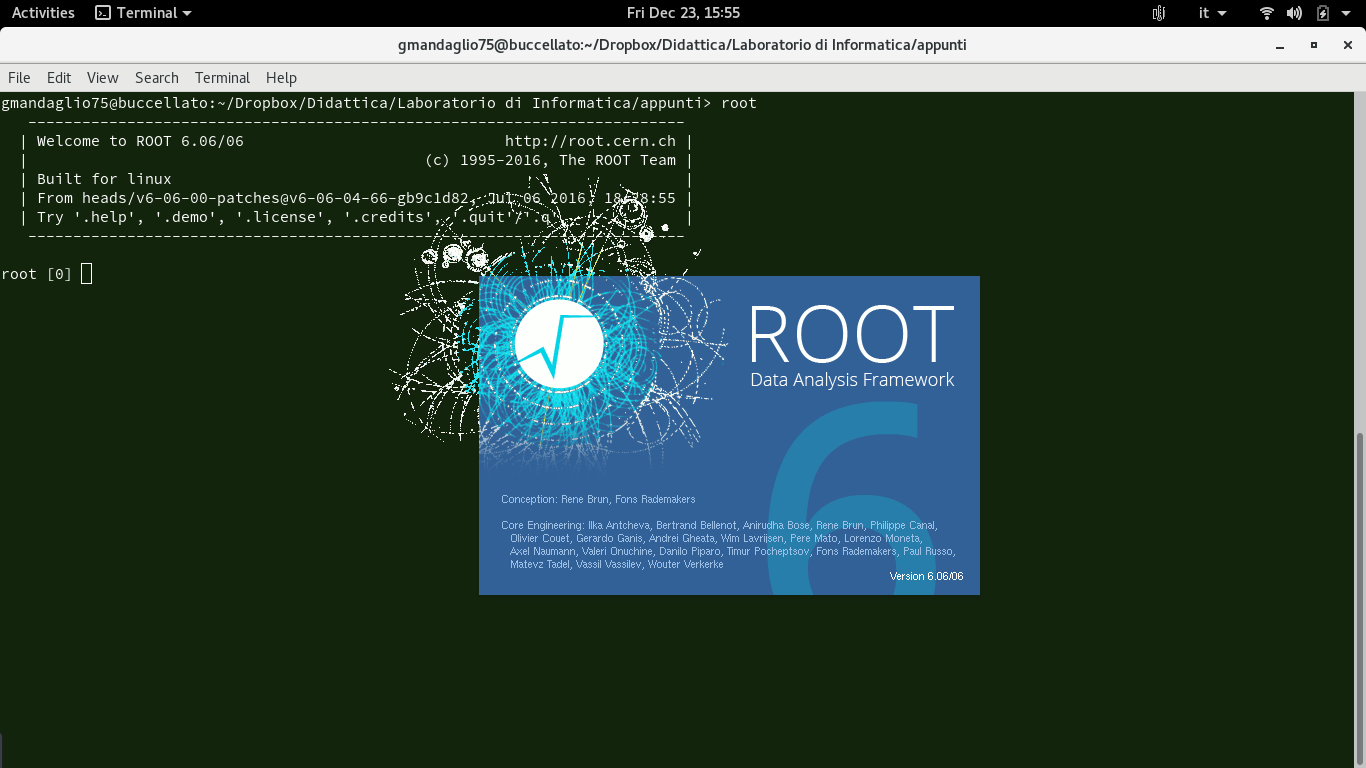
\includegraphics[scale=0.2]{start.png}
\caption{screenshot dello start di root da riga di comando.}
\end{figure}

Dalla console interattiva di root possiamo parlargli in C++, invocando una qualunque delle sue classi. Nella prossima figura, si può vedere il risultato di una breve chat con root:

\begin{figure}[h]
\centering
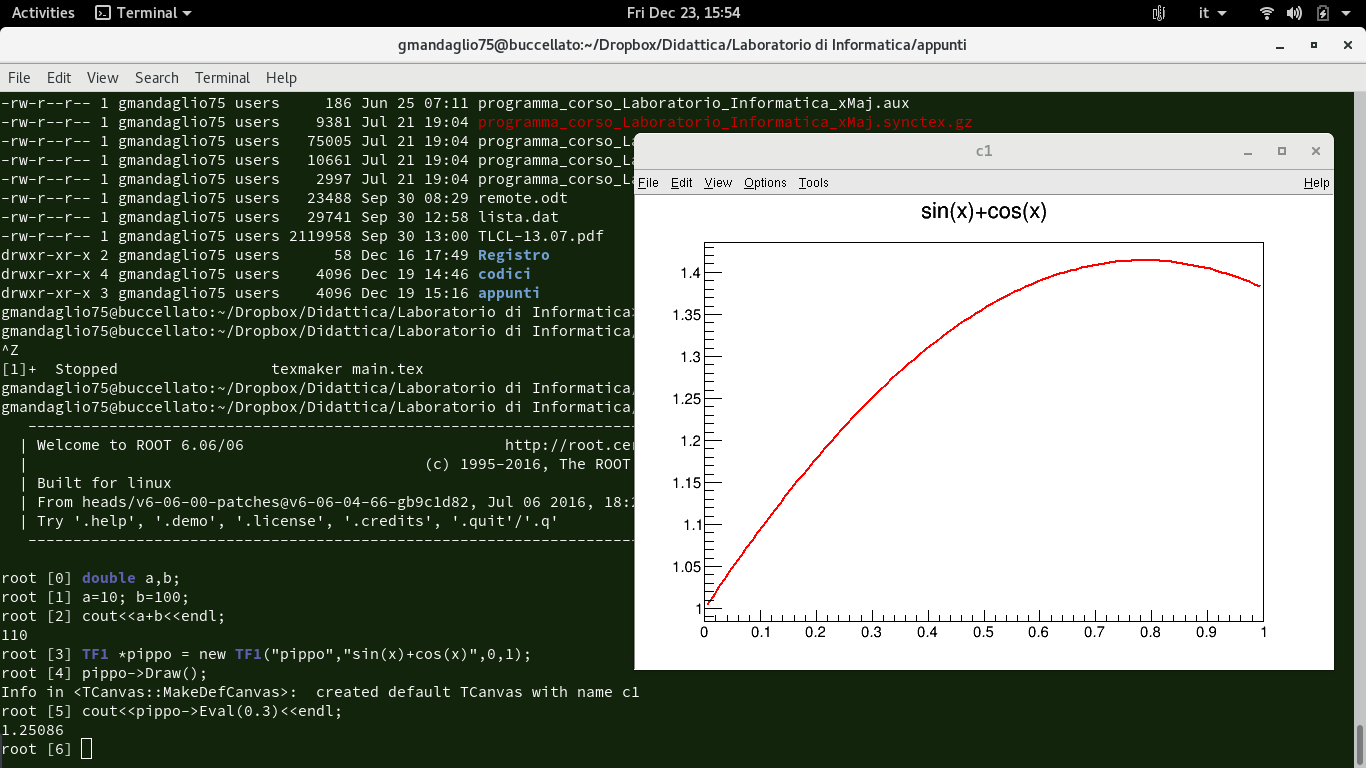
\includegraphics[scale=0.2]{chat_root.png}
\caption{screenshot di una breve chat con root e delle sue reazioni.\label{chat}}
\end{figure}

Nella chat mostrata in figura \ref{chat} si nota che sono state definite due variabili di tipo double, sono stati assegnati due valori, è stata stampato a schermo il risultato delle somma di dette variabili; è stato creato un oggetto relativo alla classe TF1 di root il cui indirizzo è memorizzato nel puntatore pippo, la creazione dell'oggetto è stato effettuato attraverso il costruttore che passa alla classe il nome dell'oggetto, la parametrizzazione della formula di una funzione, l'intervallo in cui è definita la funzione; poi è stato utilizzato il metodo Draw della classe per far apparire il grafico della funzione; stampiamo a schermo il valore della funzione stimata per $x=0.3$ attraverso il metodo Eval di TF1.

Ovviamente l'utilizzo di root come fosse una calcolatrice che parla in C++ da riga di comando è comodo e rapido ma non è il solo modo di utilizzarlo.
E' possibile scrivere dentro un file una serie di comandi racchiusi tra due graffe (script) o implementare delle funzioni, caricarle e farle eseguire a root. Di questo parleremo nel prossimo paragrafo. 


\section{Script e functions}

Proviamo a ricopiare il carteggio di cui parlavamo nel paragrafo precedente in un file con estensione .C nel seguente modo:

\begin{verse}
//script carteggio.C
{
double a,b;
a=10; b=100;
cout<<a+b<<endl;
TF1 *pippo = new TF1("pippo","sin(x)+cos(x)",0,1);
pippo->Draw();
cout<<pippo->Eval(0.3)<<endl;
}
\end{verse}

a questo punto per far eseguire lo script a root basta scrivere su terminale nella cartella dove si trova il file script \textbf{root carteggio.C} e poi invio e lui produrrà ciò che si vede in figura \ref{quantosegue}


\begin{figure}[h]
\centering
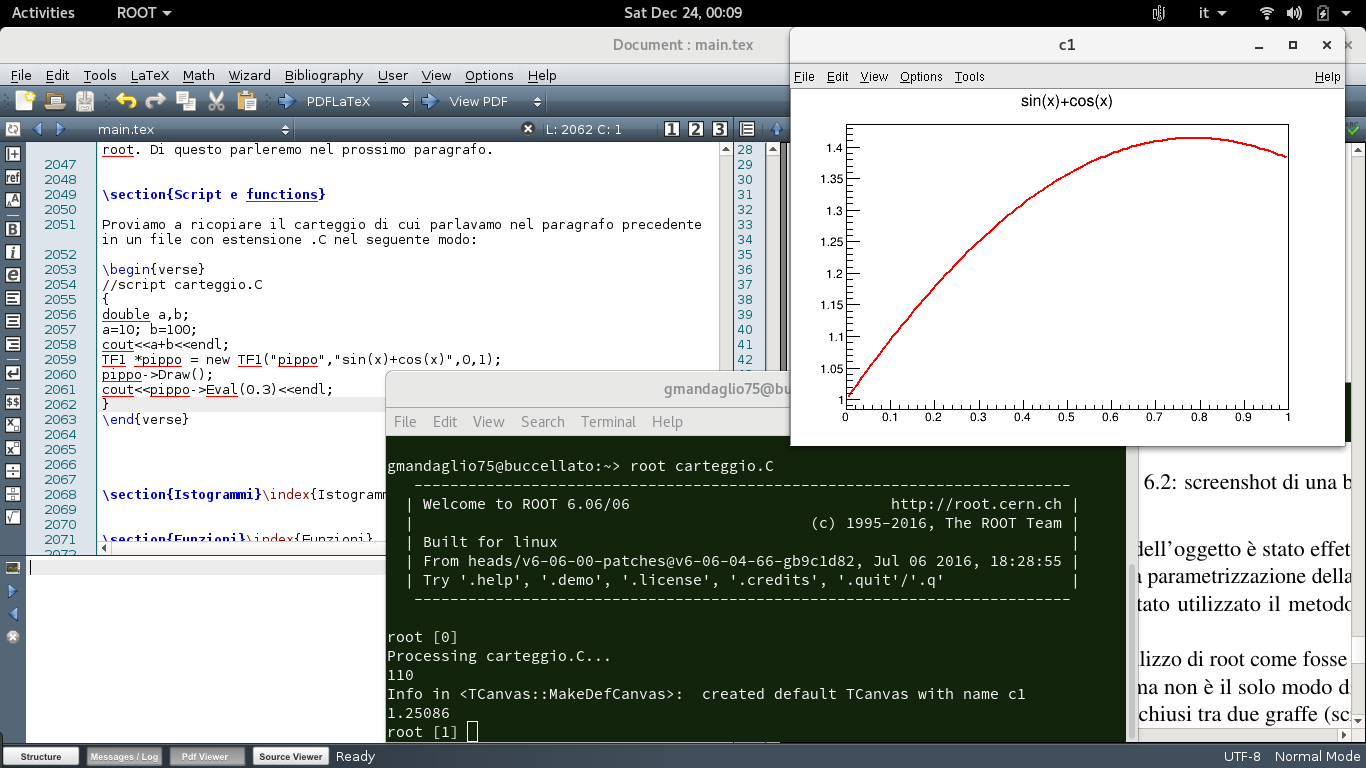
\includegraphics[scale=0.2]{quantosegue.png}
\caption{screenshot dell'operazione \textbf{root carteggio.C}.\label{quantosegue}}
\end{figure}

\'E possibile ottenere lo stesso risultato lanciando \textbf{root} e poi scrivendo sul terminale di root \textbf{.x carteggio.C} e poi invio.

root parla in C++, lo ripeto per l'ennesima volta e come esercizio facciamo ora vedere come un codice scritto in questo corso per la computazione di un istogramma puo' essere facilmente essere convertito in uno script interpretabile da root. 

\begin{verbatim}
//script prova.C
{
int i=0;
double a;
int num_dati=0;  				
float media;			
double somma=0; 		
double somm=0;		
double sqm; 			
char nome[20];

cout<<"Mi dici il nome del file dei dati?"<<endl;
cin>>nome;  

//calcola la somma e la media
ifstream leggimi(nome);        
while(!leggimi.eof()){  
	leggimi>>a;			
	somma=somma+a;
	if(!leggimi.eof()){						
		num_dati++;
	}
}
media = somma /num_dati;	
cout<<endl;
cout<<"Hai stampato "<<num_dati<<" numeri."<<endl;
cout<<"La somma dei numeri stampati e' "<<somma<<".\n";
cout<<"La media dei numeri stampati e' "<<media<<" \n";

leggimi.clear(); 
leggimi.seekg(0); 
float *misure = new float[num_dati];
for(i=0; i<num_dati; i++){
	leggimi>>misure[i];
	somm=somm+pow((misure[i]-media),2);
}
sqm=pow((somm/num_dati), 0.5);	
cout<<"Lo scarto quadratico medio e' "<<sqm<<".\n";

//restituisce il valore massimo e il valore minimo

float maxi, mini;
maxi=misure[0];
mini=misure[0];
for(i=0; i<num_dati; i++){			
	if(misure[i]>maxi){
		maxi=misure[i];
	}
	else if(misure[i]<mini){
	mini=misure[i];
	}
}

cout<<"Il valore minimo e': "<<mini<<endl;
cout<<"Il valore massimo e': "<<maxi<<endl;

//creare istogramma
int r;
cout << fixed; 
do{	
	int nint;					
	cout<<"\nInserisci il numero di intervalli dell'istogramma: \n";
	cin>>nint;
	float l=(maxi-mini)/(float)nint;					
	cout<<"Misura intervalli: "<<l<<endl;
	int bin[nint];					
	for(i=0;i<nint;i++){	   
		bin[i]=0;  
	}  
	for(i=0;i<nint;i++){
 		for(int v=0; v<num_dati; v++){ 
			if((misure[v]>=mini+i*l)&&(misure[v]<=mini+(i+1)*l)){   
				bin[i]++;
			} 
		}
	}
    cout<<"\nIstogramma:"<<endl;
	for(int n=0; n<nint; n++){ 		
	cout<<mini+l/2+n*l<<"\t"<<bin[n]<<endl;          
	}
	cout<<"\n Istogramma con nuovo binning? (Si? Premi 1):\n";
	cin>>r;
}while(r==1);
}
\end{verbatim}

Come si può vedere abbiamo tagliato solo la testa del programma con le chiamate agli header files e la definizione della funzione principale, abbiamo lasciato solo il corpo della funzione principale racchiusa tra due parentesi graffe. In figura \ref{scriptino} si può vedere lo script in azione attraverso l'interprete fornito da root:
\begin{figure}[h]
\centering
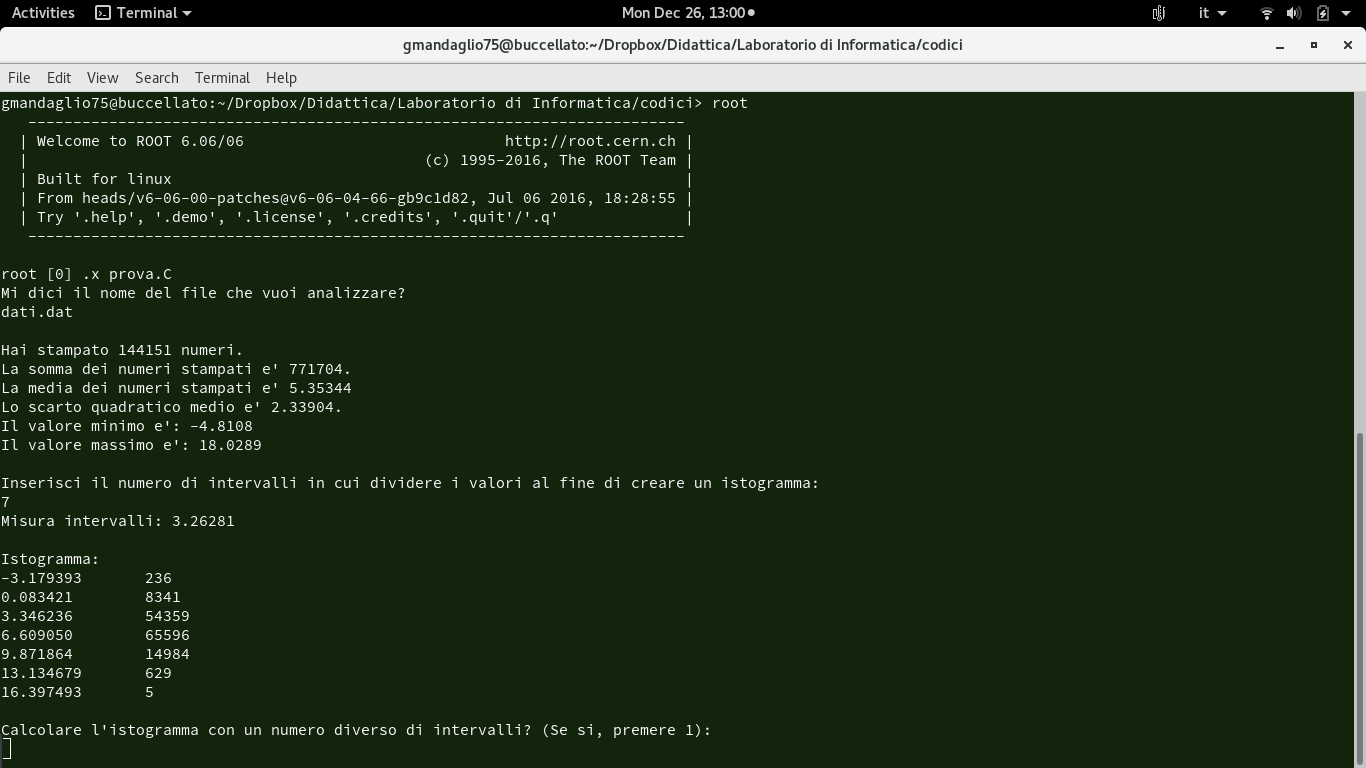
\includegraphics[scale=0.2]{scriptino.png}
\caption{screenshot dell'operazione \textbf{root carteggio.C}.\label{scriptino}}
\end{figure}

Lo stesso risultato lo avremmo potuto realizzare attribuendo il corpo del precedente script a una funzione, nel seguente modo:

\begin{verbatim}
//script prova.C
istogrammami()
{
int i=0;
double a;
int num_dati=0;  				
float media;	
.....;
..tutto paro paro come sopra ;)
.....;
.....; //etc
	cout<<"\n Istogramma con nuovo binning? (Si? Premi 1):\n";
	cin>>r;
}while(r==1);
return;
}
\end{verbatim}

Abbiamo scritto una funzione di nome istogrammami che non restituisce nessun valore e che ha come corpo lo script precedente.
\begin{figure}[h]
\centering
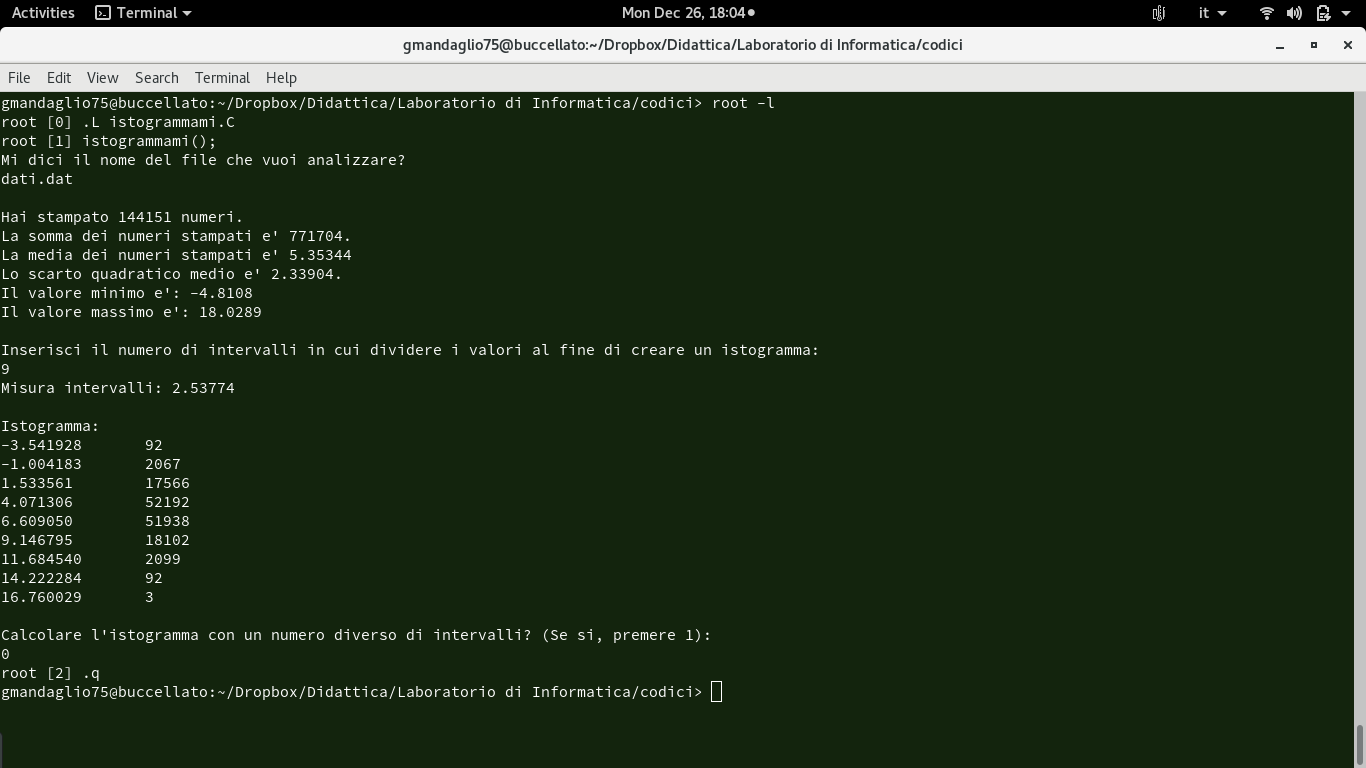
\includegraphics[scale=0.2]{funzione.png}
\caption{ Screenshot del caricamento ed esecuzione di una funzione con root.\label{funzione}}
\end{figure}

Per lanciare una funzione da root, prima lo apriamo, carichiamo la funzione con il comando \textbf{.L istogrammami.C} (la L sta per link), poi si fa girare la funzione invocandola come faremmo in un normale programma C++ \textbf{istogrammami();}.
Anche nel caso delle funzioni come negli script non è necessario caricare gli header file come faremmo in un programma C++ compilato. root apparecchia di tutto il necessario, il nostro codice e il suo interprete fanno il resto.

\section{Istogrammi}\index{Istogrammi}
Nel paragrafo \ref{istocostr} abbiamo speso un po' di parole su cosa siano gli istogrammi e quale importanza abbiano nell'analisi statistica dei dati.
Abbiamo inoltre imparato a costruire un istogramma partendo dai dati grezzi implementando un codice in C++.

In questo paragrafo vedremo come root fornisca una serie di classi per la costruzione, la visualizzazioni e  le operazioni su istogrammi mono- bi- e tri- dimensionali.
Le classi\footnote{https://root.cern.ch/root/html516/TH1D.html} preposte allo scopo sono:
\begin{itemize}
\item Istogrammi 1D:
\begin{itemize}
\item TH1C : Istogrammi con un \textit{byte} per canale. Massimo valore per \textit{bin}= 127
\item    TH1S : Istogrammi con un \textit{short} per canale. Massimo valore per \textit{bin}=  32767
\item    TH1I : Istogrammi con un \textit{int} per canale. Massimo valore per \textit{bin}=  2147483647
\item    TH1F : Istogrammi con un \textit{float} per canale. Precisione massima 7 \textit{digits}
\item    TH1D : Istogrammi con un \textit{double} per canale. Precisione massima 14 \textit{digits} 
\end{itemize}
\item Istogrammi 2D:
\begin{itemize}
\item     TH2C : Istogrammi con un  \textit{byte} per canale. Massimo valore per \textit{bin}=  127
\item     TH2S : Istogrammi con un  \textit{short} per canale. Massimo valore per \textit{bin}=  32767
\item     TH2I : Istogrammi con un  \textit{int} per canale. Massimo valore per \textit{bin}=  2147483647
\item     TH2F : Istogrammi con un  \textit{float} per canale. Precisione massima 7 \textit{digits}
\item     TH2D : Istogrammi con un  \textit{double} per canale. Precisione massima 14 \textit{digits} 
\end{itemize}

\item Istogrammi 3D:
\begin{itemize}
\item     TH3C : Istogrammi con un  \textit{byte} per canale. Massimo valore per \textit{bin}=  127
\item     TH3S : Istogrammi con un  \textit{short} per canale. Massimo valore per \textit{bin}=  32767
\item     TH3I : Istogrammi con un  \textit{int} per canale. Massimo valore per \textit{bin}=  2147483647
\item     TH3F : Istogrammi con un  \textit{float} per canale. Precisione massima 7 \textit{digits}
\item     TH3D : Istogrammi con un  \textit{double} per canale. Precisione massima 14 \textit{digits} 
    \end{itemize}
\end{itemize}

Uno dei tanti costruttori per inizializzare un istogramma 1D ha questa forma:
\begin{verbatim}
TH1D (const char *name, const char *title, Int_t nbinsx, Double_t xlow, Double_t xup)
\end{verbatim}
dove le espressioni \textbf{Int\_t}, \textbf{Double\_t} si intende i tradizionali interi e reali a doppia precisione del C++, la scrittura differente è introdotta da root in modo da rendere il codice machine-independent, ovvero adatta il tipo di dato alla piattaforma hardware sulla quale dovrà essere eseguito il codice.
Il paradigma del costruttore appena mostrato richiede: il nome dell'oggetto che sarà memorizzato nella stringa \textit{name}, il titolo dell'istogramma nella stringa \textit{title}, il numero di bin ovvero il numero di intervalli dell'istogramma \textit{nbinsx}, gli estremi dell'istogramma \textit{xlow} e \textit{xup}.

La classe dispone di una grande varietà di metodi: per caricare i dati \textit{Fill}, per produrre un grafico \textit{Draw}, per gestire la rappresentazione dell'istogramma, effettuare fit etc.

Di seguito quattro righe di codice per rappresentare con un istogramma i dati raccolti in un esperimento nel corso di Laboratorio di Fisica 1 A;
l'esperimento consisteva nella misura del diametro di biglie di plastica effettuate con un calibro. I dati sono stati trascritti in un file (Misure.dat).

\begin{verbatim}
{
   TH1F *pippo = new TH1F("pippo"," ",10,3.6,4);
   ifstream leggimi("Misure.dat");
   double a;
   while(!leggimi.eof()){
   leggimi>>a;
   if(!leggimi.eof()){
     pippo->Fill(a);
    }
    }
    pippo->Draw();
    //consente di salvare la figura in formato pdf
    c1->SaveAs("grezzo.pdf");
}
\end{verbatim}

Il risultato che viene prodotto dall'interpretazione delle quattro righe di codice appena scritte è mostrato in figura \ref{grezzo}.
Una prima cosa che possiamo notare è che il codice che abbiamo scritto per costruire un istogramma nel paragrafo \ref{istocostr} può essere sostituito da una classe \textbf{TH1D} che risolve il problema in un modo molto generale e fornendo molte più funzionalità come quella grafica come possiamo vedere in questo esempio attraverso il metodo \textit{Draw}.
\begin{figure}
\centering
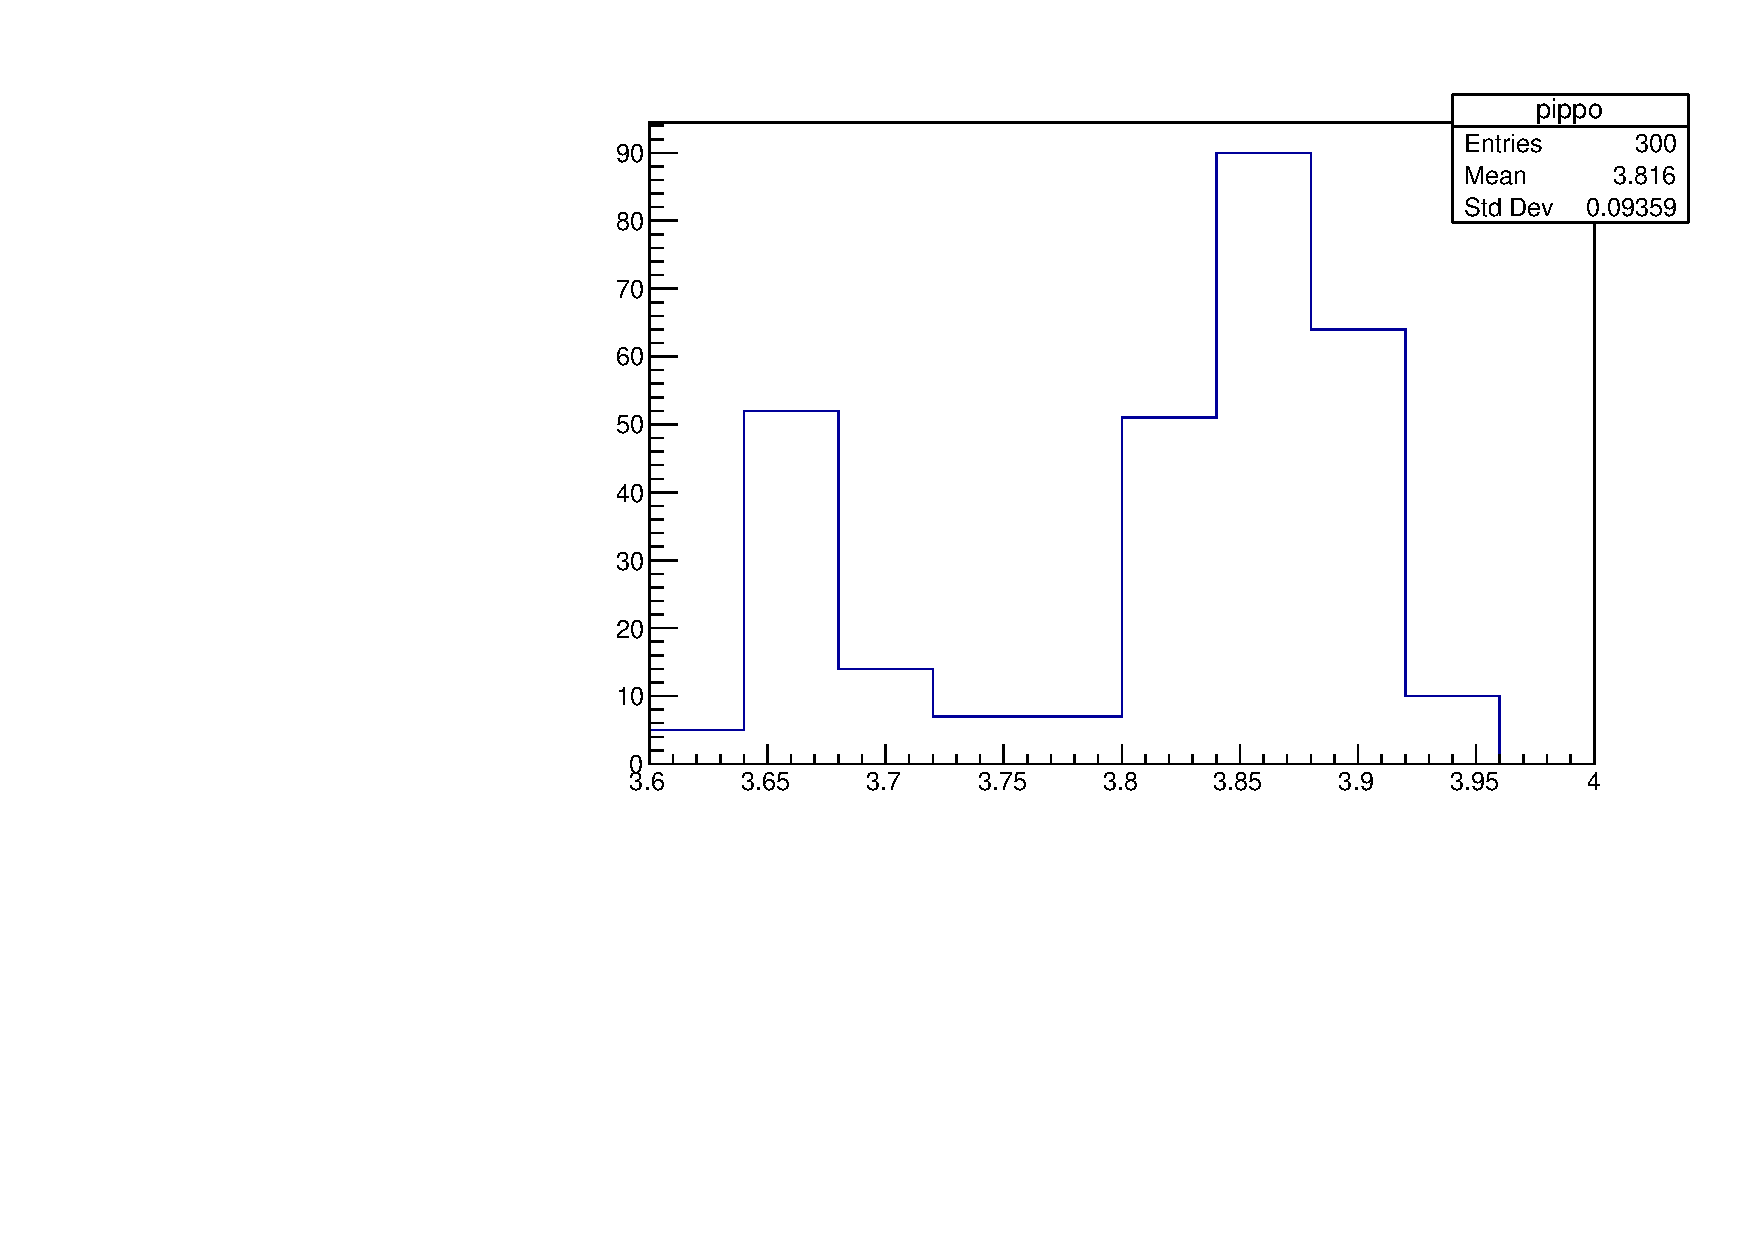
\includegraphics[scale=0.5]{grezzo.pdf}
\caption{Istogramma computato dall'oggetto pippo della classe TH1D.\label{grezzo}}
\end{figure}

Di seguito mostreremo uno script che nella sostanza fa le stesse cose dello script appena scritto e descritto, ma che contiene un numero di istruzioni maggiori, che servono semplicemente a rendere la presentazione dei nostri dati più ordinata e decorosa, pronta ad essere inclusa in una relazione del lavoro svolto.
\begin{verbatim}
{
 int mymarkerstyle=20;
 float mymarkersize=1.;
 float mytextsize=0.065;
 int mytextfont=132;

 TCanvas *Canvas_1 = new TCanvas("Canvas_1", "Canvas_1",600,500);
 gStyle->SetOptStat("");
 Canvas_1->SetFillColor(0);
 Canvas_1->SetBorderMode(0);
 Canvas_1->SetBorderSize(2);
 Canvas_1->SetLeftMargin(0.18);
 Canvas_1->SetRightMargin(0.12);
 Canvas_1->SetTopMargin(0.03);
 Canvas_1->SetBottomMargin(0.16);
 Canvas_1->SetTickx(1);
 Canvas_1->SetTicky(1);
 
////ZOOM SCATOLA////////////////////////////////////
   TH2F *hpx = new TH2F("hpx"," ",10,3.6,4,10,0.,100);
   hpx->SetStats(0);
   hpx->SetNdivisions(905);
   hpx->GetXaxis()->SetTitleSize(mytextsize);
   hpx->GetYaxis()->SetTitleSize(mytextsize);
   hpx->GetXaxis()->SetLabelSize(mytextsize);
   hpx->GetYaxis()->SetLabelSize(mytextsize);
   hpx->GetXaxis()->SetTitleFont(mytextfont);
   hpx->GetYaxis()->SetTitleFont(mytextfont);
   hpx->GetXaxis()->SetLabelFont(mytextfont);
   hpx->GetYaxis()->SetLabelFont(mytextfont);
   hpx->GetYaxis()->CenterTitle(1);
   hpx->GetXaxis()->CenterTitle(1);
   hpx->GetYaxis()->SetTitleOffset(1.2);
   hpx->GetXaxis()->SetTitleOffset(1.10);
   hpx->SetTitle("");
   hpx->GetYaxis()->SetTitle("Conteggi");
   hpx->GetXaxis()->SetTitle("Diametro Palline (mm)");
   hpx->Draw();
/////////////////////////////////////////////////////////////////////

   TH1F *pippo = new TH1F("pippo"," ",10,3.6,4);
   pippo->SetLineWidth(2);
   pippo->SetLineColor(1);
   ifstream leggimi("Misure.dat");
   double a;
   while(!leggimi.eof()){
   leggimi>>a;
   if(!leggimi.eof()){
     pippo->Fill(a);
    }
    }
    pippo->Draw("same");

   Canvas_1->SaveAs("palline.pdf");
}
\end{verbatim}
Descriviamo brevemente lo script un po' meno scarno del primo:
la classe \textbf{TCanvas} gestisce la scatola in cui vivrà la nostra figura, l'istogramma 2D \textit{hpx} serve per creare una figura finta sulla quale sovrapporre l'istogramma con i nostri dati, infine usiamo la classe \textbf{TH1D} per caricare i dati e modificarne l'aspetto attraverso i metodi \textit{SetLineWidth} e \textit{SetLineColor} che cambiano lo spessore e il colore della linea. Il risultato di questo script è mostrato nella figura \ref{menogrezzo}.
\begin{figure}
\centering
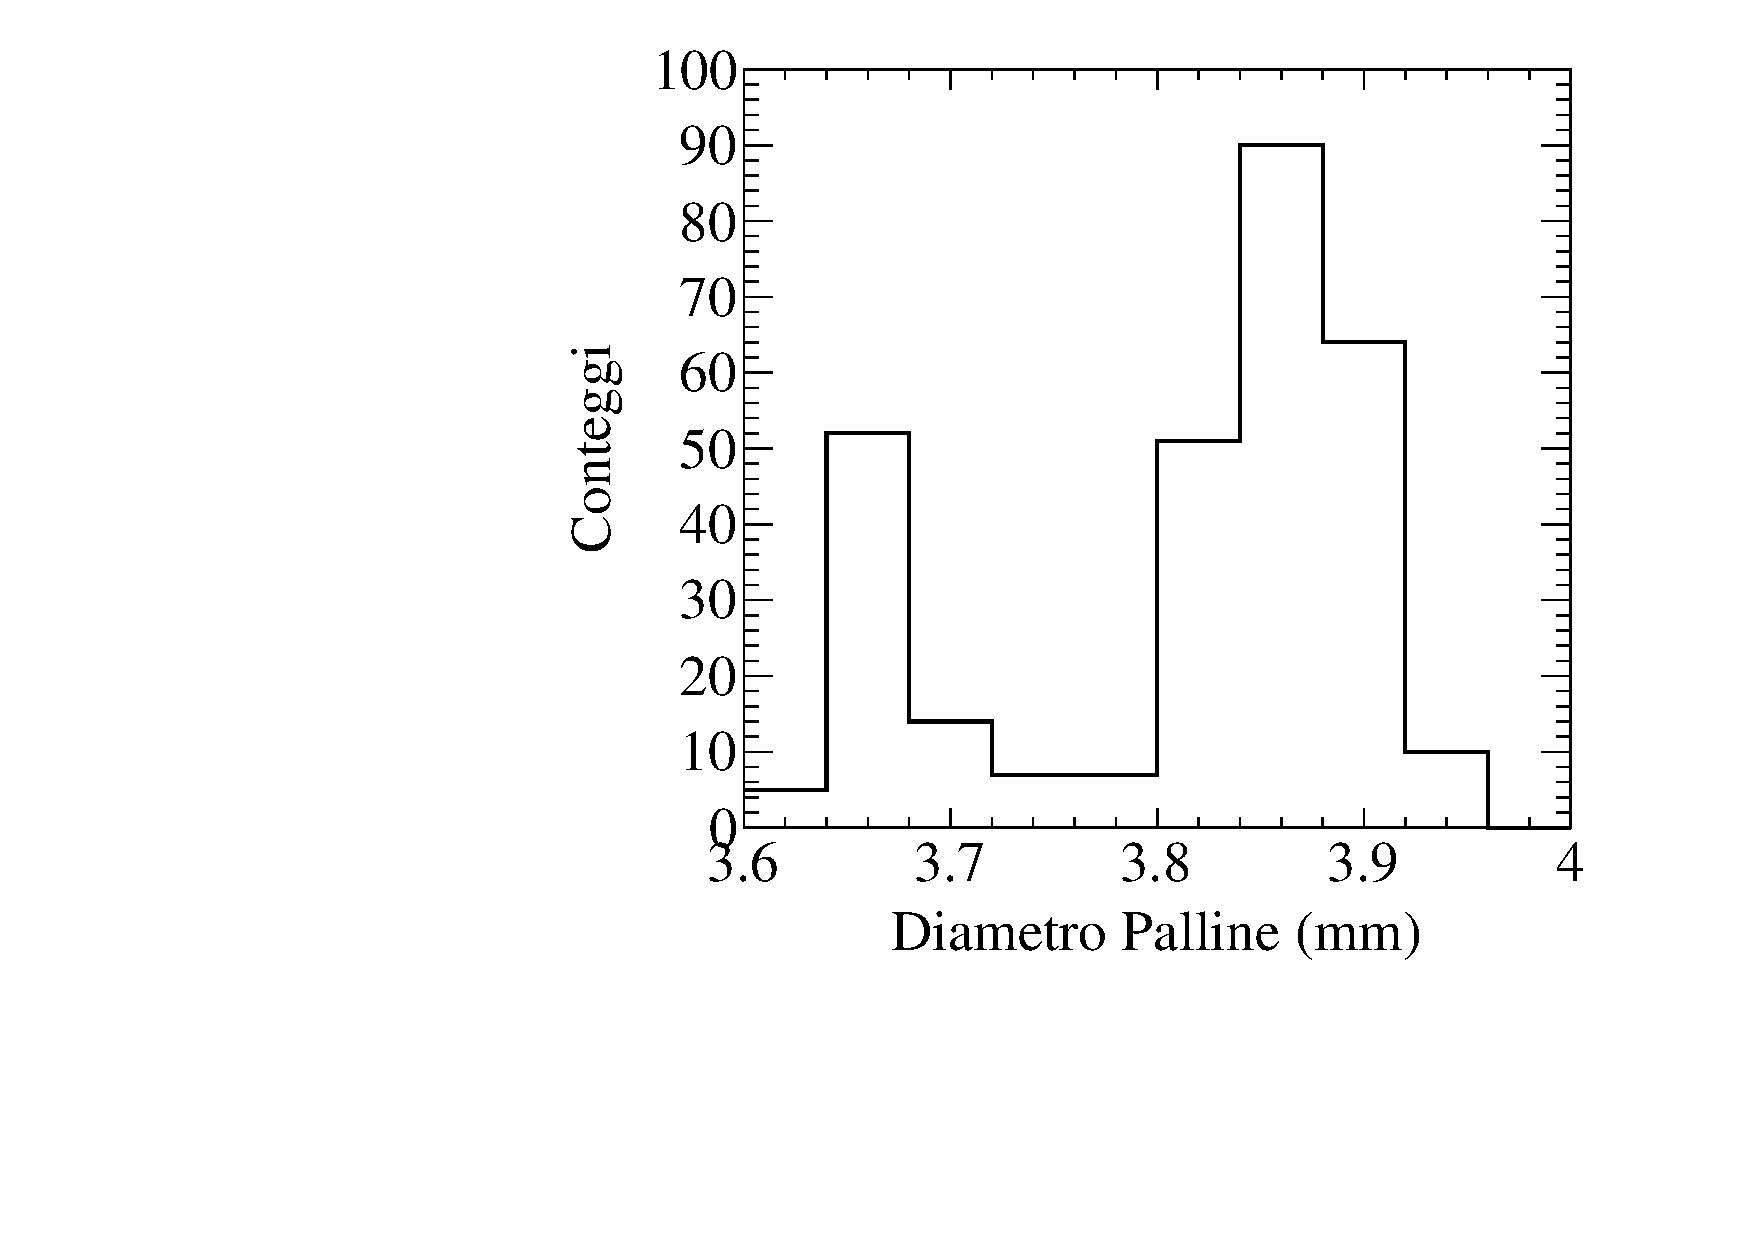
\includegraphics[scale=0.5]{palline.pdf}
\caption{Istogramma computato dallo script un po meno scarno.\label{menogrezzo}}
\end{figure}

Ripetiamo l'esperimento misurando la lunghezza di 2000 chiodi da 7 cm. L'esperimento è identico al precedente, cambia solamente il soggetto della misura e la sua numerosità. A parte il divertimento e le ore necessarie nella misura di ciascun chiodo, l'analisi dei dati risulta immediata reciclando il codice scritto per l'esperimento delle palline. \'E sufficiente modificare gli estremi dell'istogramma, il titolo degli assi e il risultato può essere osservato in figura \ref{chiodi}.


\begin{figure}
\centering
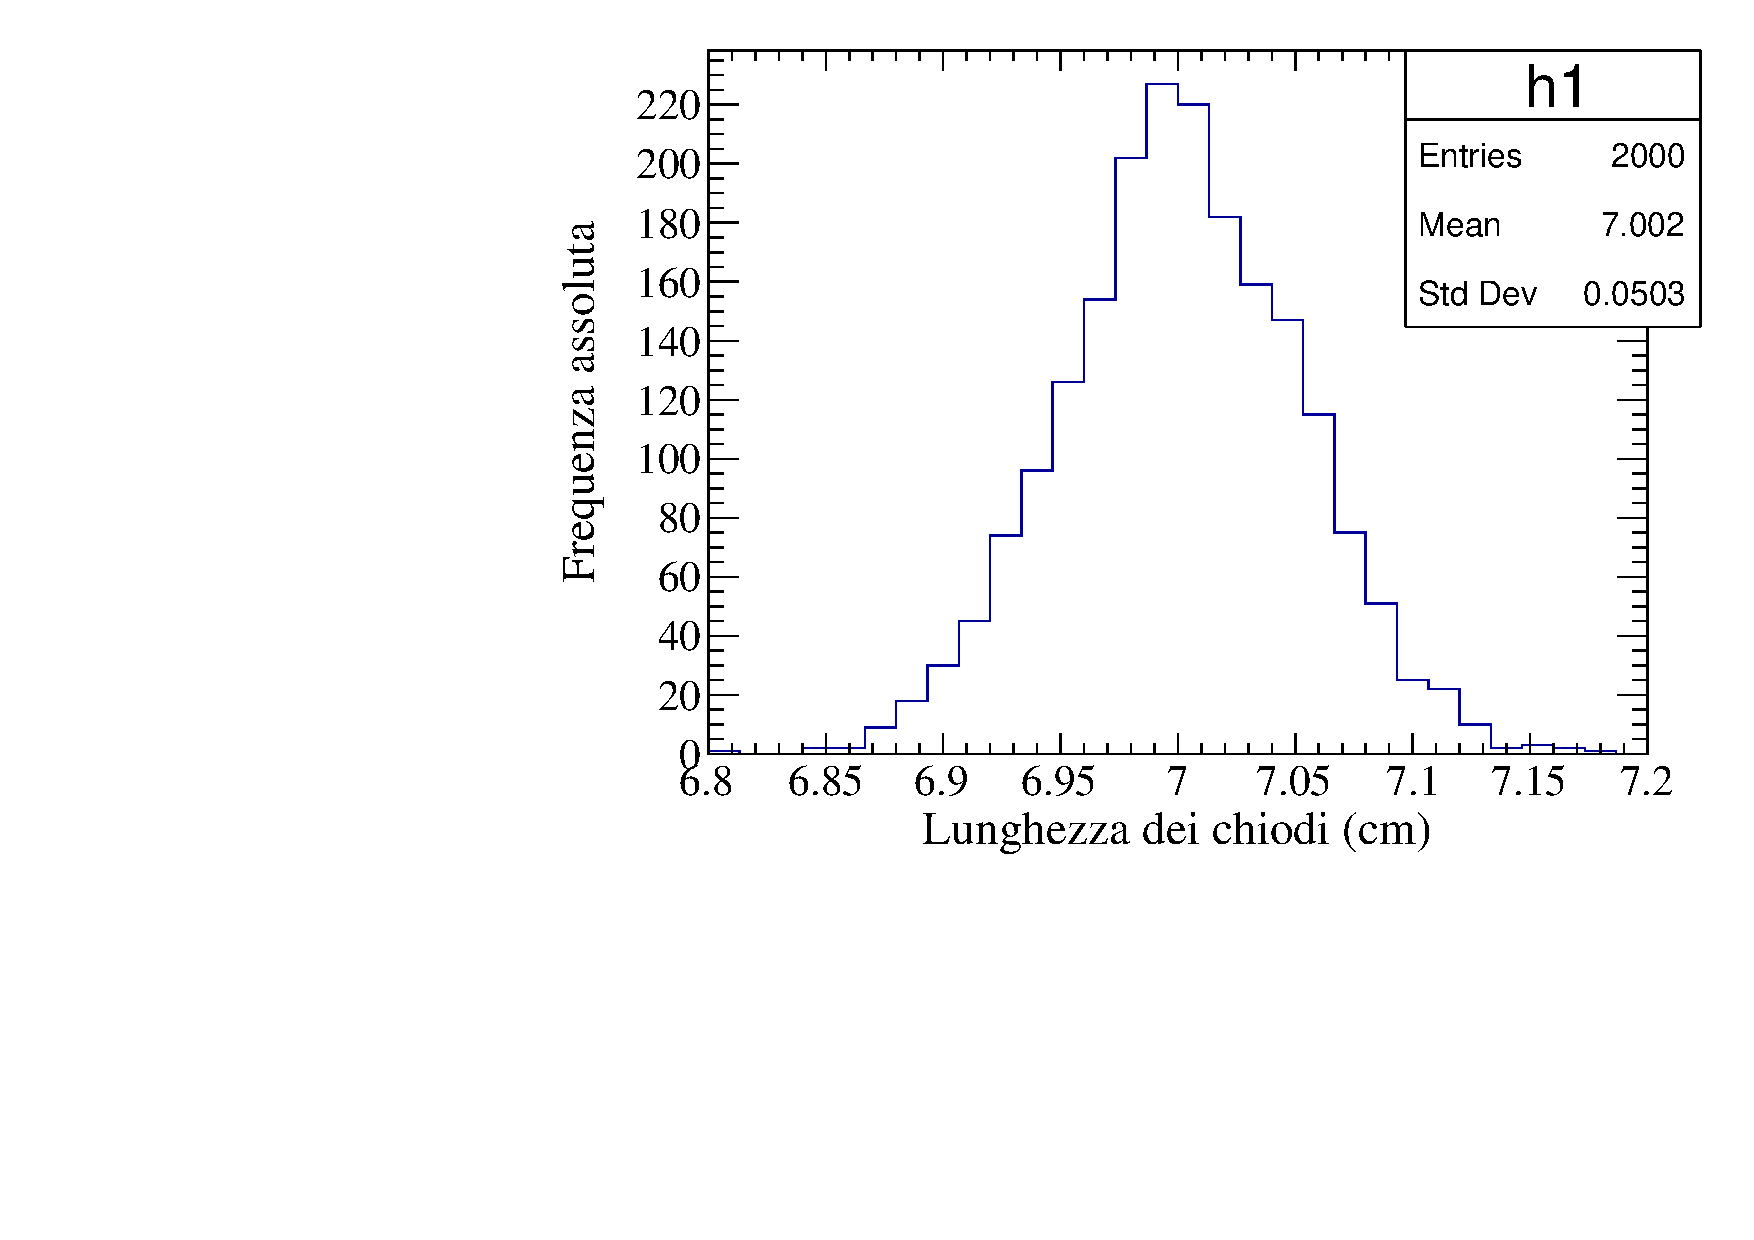
\includegraphics[scale=0.35]{chiodiist.pdf}
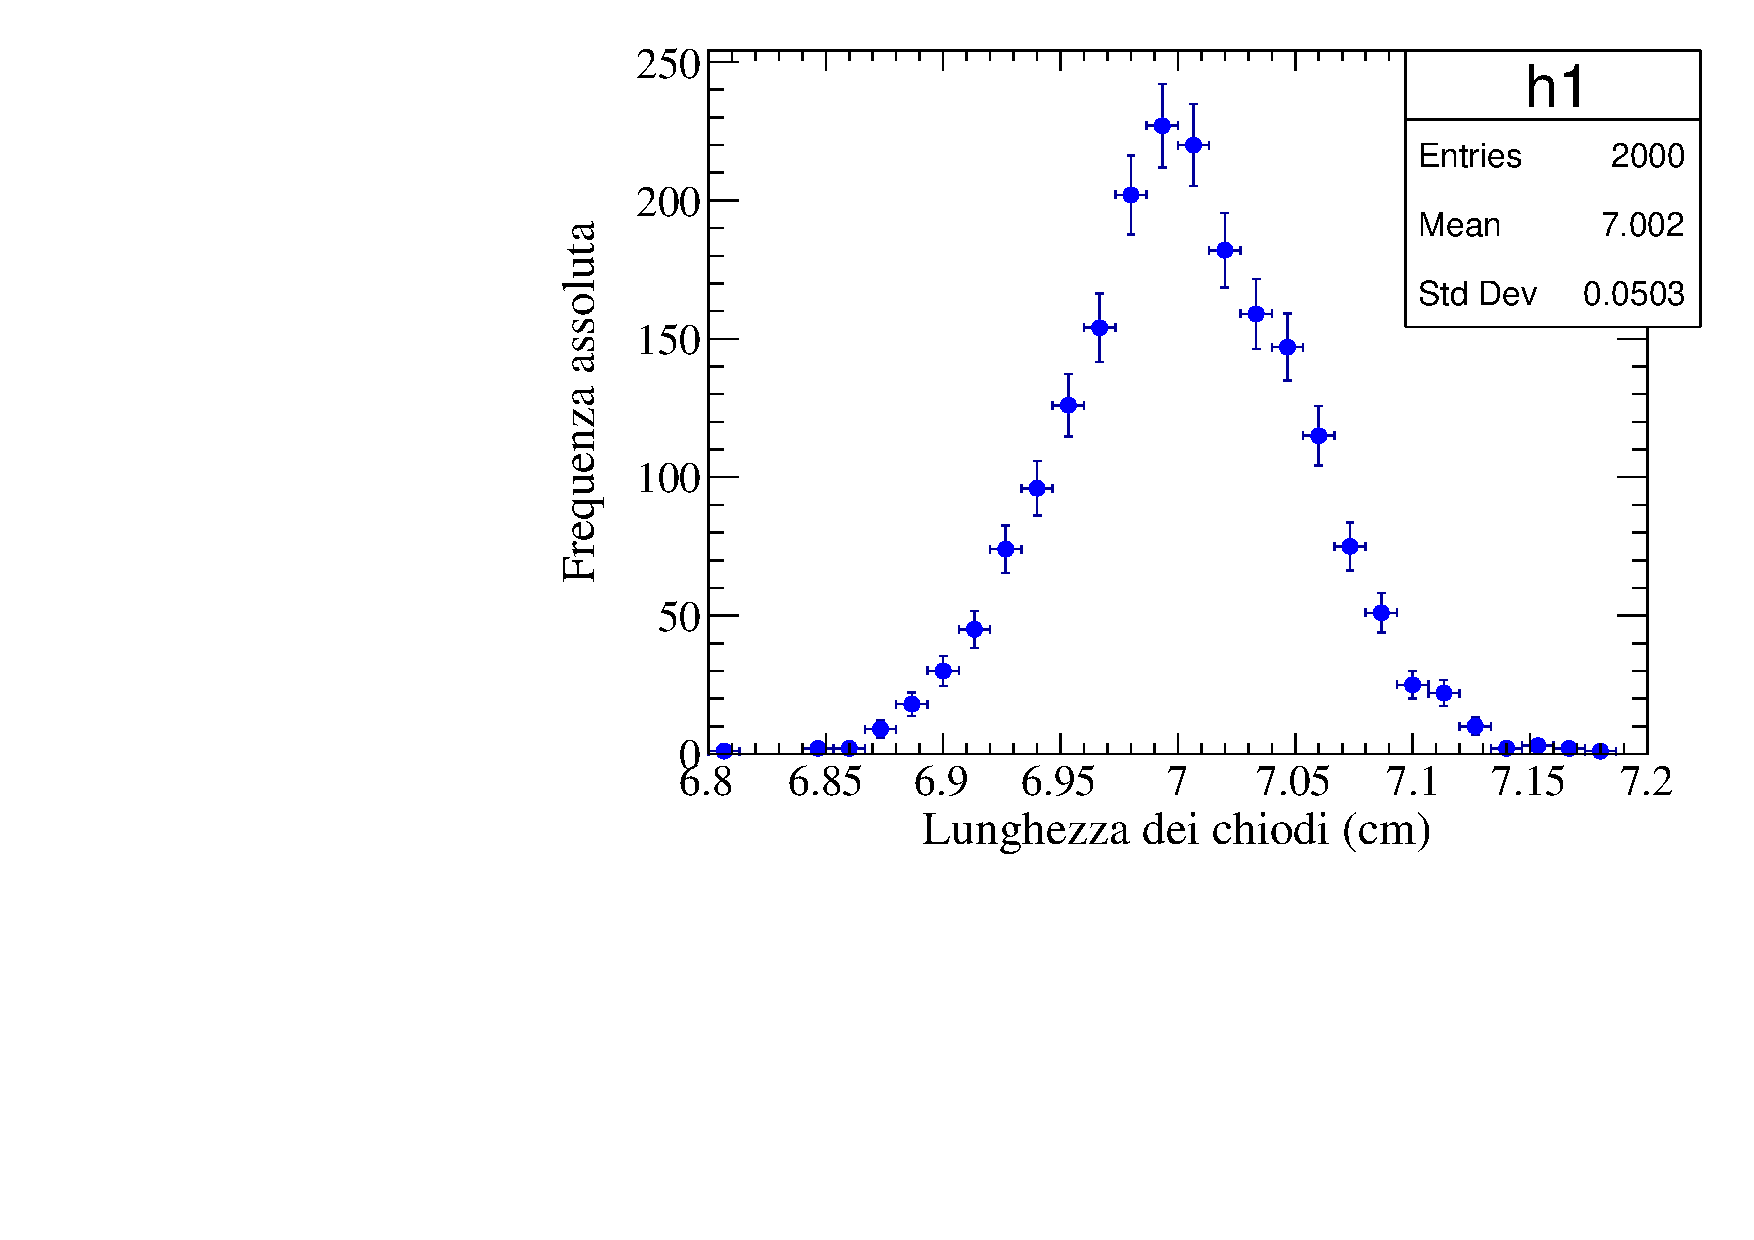
\includegraphics[scale=0.35]{chiodiistp.pdf}
\caption{Istogrammi esperimento dei chiodi. Sinistra rappresentazione equivalente dell'istogramma, ogni punto fornisce la frequenza assoluta, l'errore sulla lunghezza è legato alla larghezza del bin, l'errore sull'altezza è l'errore statistico (la radice quadrata del numero di conteggi dell'istogramma).\label{chiodi}}
\end{figure}

Abbiamo detto che è possibile computare anche istogrammi bi-dimensionali.
Prima di far vedere i modi in cui possono essere visualizzati questi istogrammi, descriviamo cosa sono attraverso un semplice esempio:
immaginiamo di ripetere l'esperimento della misura della lunghezza dei chiodi e di misurare questa volta anche un'altra quantità come ad esempio il peso del chiodo o il diametro a metà lunghezza del chiodo. In questo secondo esperimento per ogni campione abbiamo due misure che lo caratterizzano. A questo punto potremmo costruire un istogramma utilizzando due quantità, l'altezza e il peso. Identifichiamo l'asse x con l'altezza e l'asse y con il peso, gli intervalli in cui dividiamo i due assi individueranno sul piano lunghezza peso delle superfici rettangolari, a questo punto possiamo usare l'asse z per contare il numero di volte che un chiodo è stato classificato appartenere ad un dato rettangolo. Questo tipo di rappresentazione può farci capire se esistono correlazioni tra le diverse misure che caratterizzano l'oggetto: il chiodo più pesante è più lungo, forse è più corto, oppure non ha legame con la lunghezza; chi può dirlo? Lo può dire l'analisi con l'istogramma 2D.

In figura \ref{bidimy} sono riportate alcuni modi di rappresentare un istogramma bidimensionale con root.


\begin{figure}
\centering
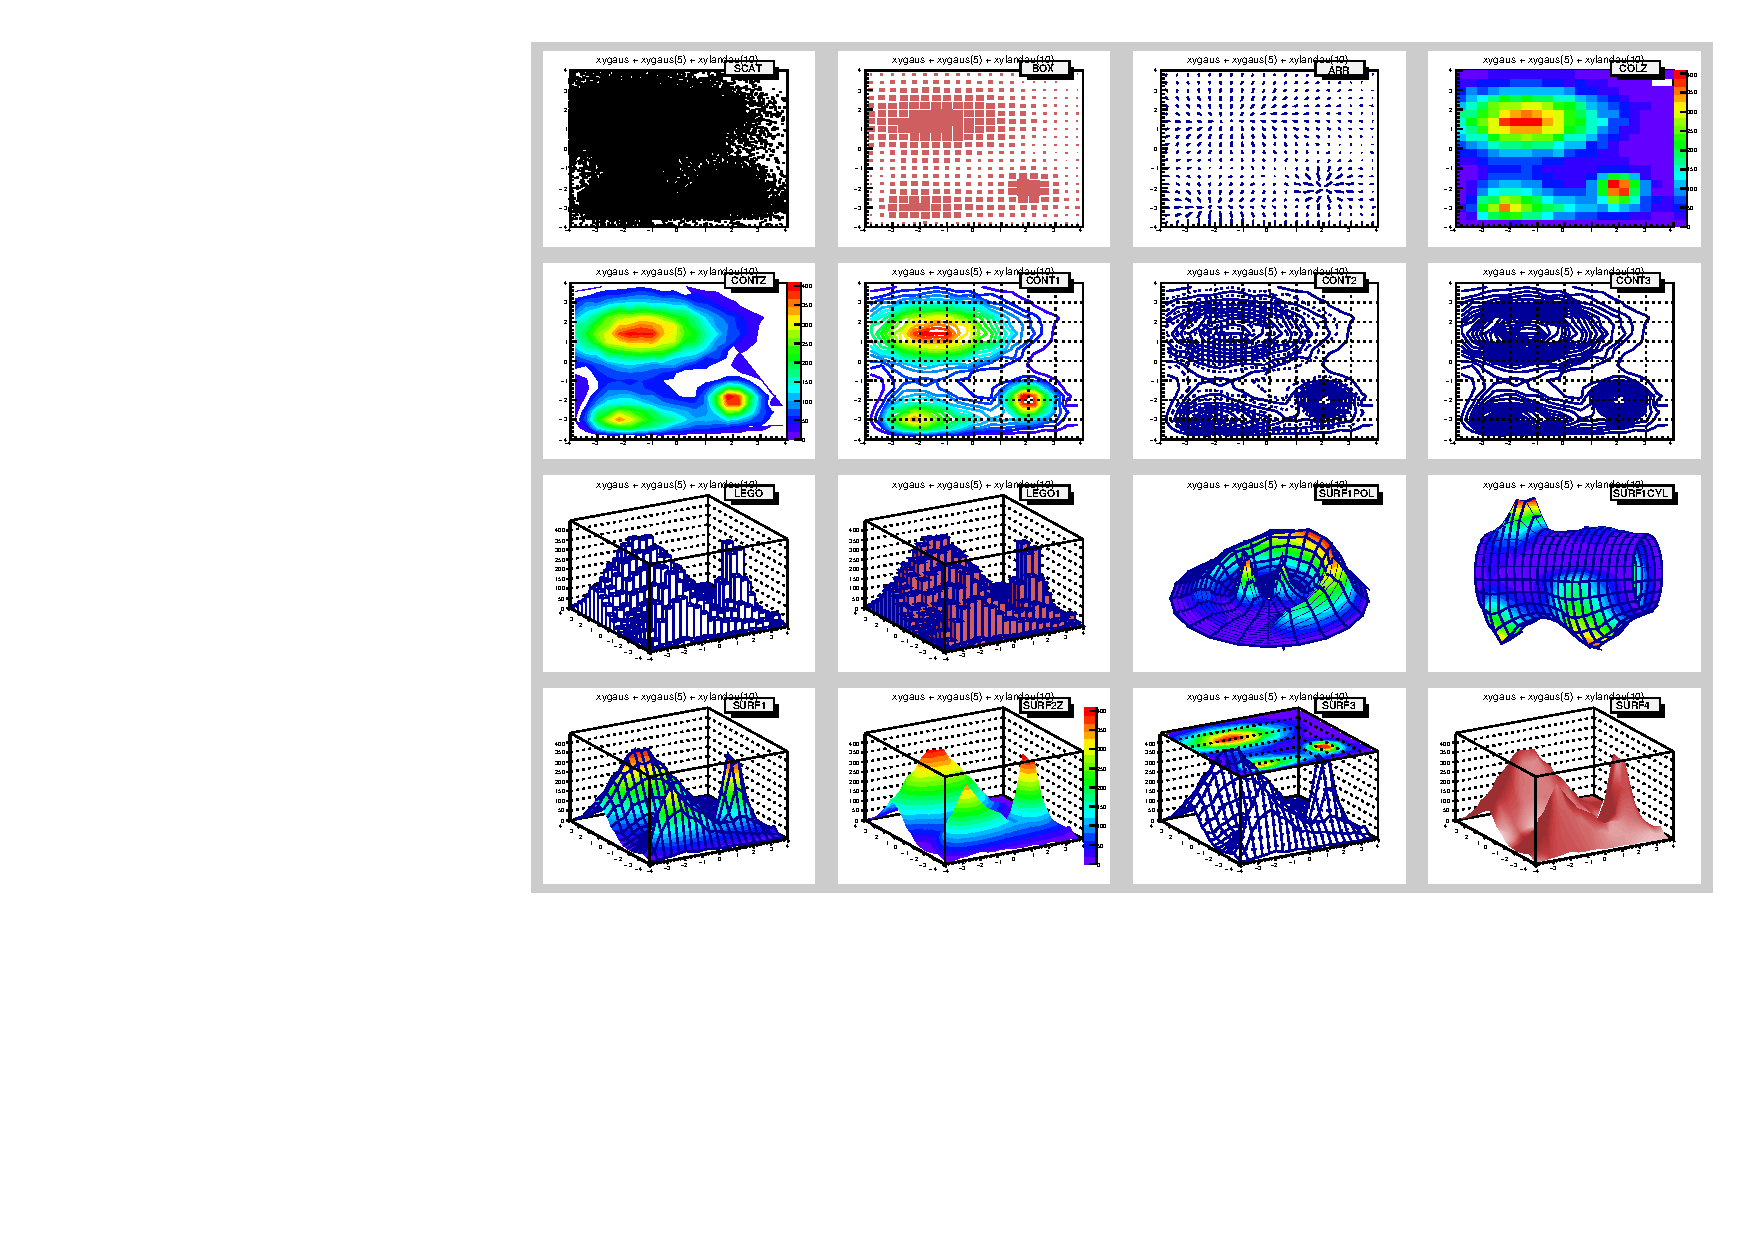
\includegraphics[scale=0.6]{miltivis.pdf}
\caption{Modi possibili per rappresentare un istogramma 2D con root.\label{bidimy}}
\end{figure}

\section{Funzioni matematiche}\index{Funzioni matematiche}

Le funzioni matematiche possono essere rappresentate attraverso le classi \textbf{TF1}, \textbf{TF2} e \textbf{TF3}, ciascuna consente di modellizzare 
funzioni di una, due o tre variabili.
Le funzioni matematiche possono essere utilizzate come modello di riferimento per effettuare dei fit oppure per generare distribuzioni di numeri con un MonteCarlo. Di seguito mostreremo alcuni esempi, ma ormai avrete capito che non avete bisogno di ulteriori aiuti, spiegazioni o suggerimenti. Considerando che root parla il C++(e son 10 volte che lo ripeto), voi ne conoscete i rudimenti, il CERN fornisce attraverso il suo sito web una larga documentazione delle sue classi e manuali sfogliabili sul web sul sito o scaricabili in formato pdf (https://root.cern/doc/master/index.html); non avete più scuse usatelo usatelo usatelo, e se scoprite cose nuove condividetele con i colleghi, e se trovate errori (bug) comunicateli ai colleghi del CERN perchè li possano correggere. 

Immaginiamo di aver sentito parlare a lezione di Fisica generale 1 del moto oscillatorio smorzato, e di esserne rimasti particolarmente colpiti essendo tutti quanti patiti di altalene, biglie, tappetini elastici, chitarre etc.
A questo punto vogliamo visualizzare le funzioni che descrivono questo tipo di fenomeno, l'esponenziale che definisce lo smorzamento e la funzione sinusoidale per le oscillazioni:
\begin{verbatim}
//script funzioni.C
{
TF1 *expy = new TF1("expy","10*exp(-x/3)",0,15);
TF1 *expyneg = new TF1("expyneg","-10*exp(-x/3)",0,15);
TF1 *expsin = new TF1("expsin","[0]*exp(-x/[1])*sin([2]*x)",0,15);
expsin->SetParameters(10,3,4);
expy->SetLineColor(1);
expy->SetLineWidth(2);
expyneg->SetLineColor(1);
expyneg->SetLineWidth(2);
expsin->SetLineColor(4);

expsin->Draw();
expy->Draw("same");
expyneg->Draw("same");
}
\end{verbatim}
In questo semplice script vediamo come scrivere un funzione in modo completo dentro il costruttore nell'oggetto \textit{expy} e come scriverla in dipendenza di parametri ($[0],[1] etc$) e come passare i valori alla funzione \textit{expsin} attraverso il metodo \textit{SetParameters}.


\begin{figure}
\centering
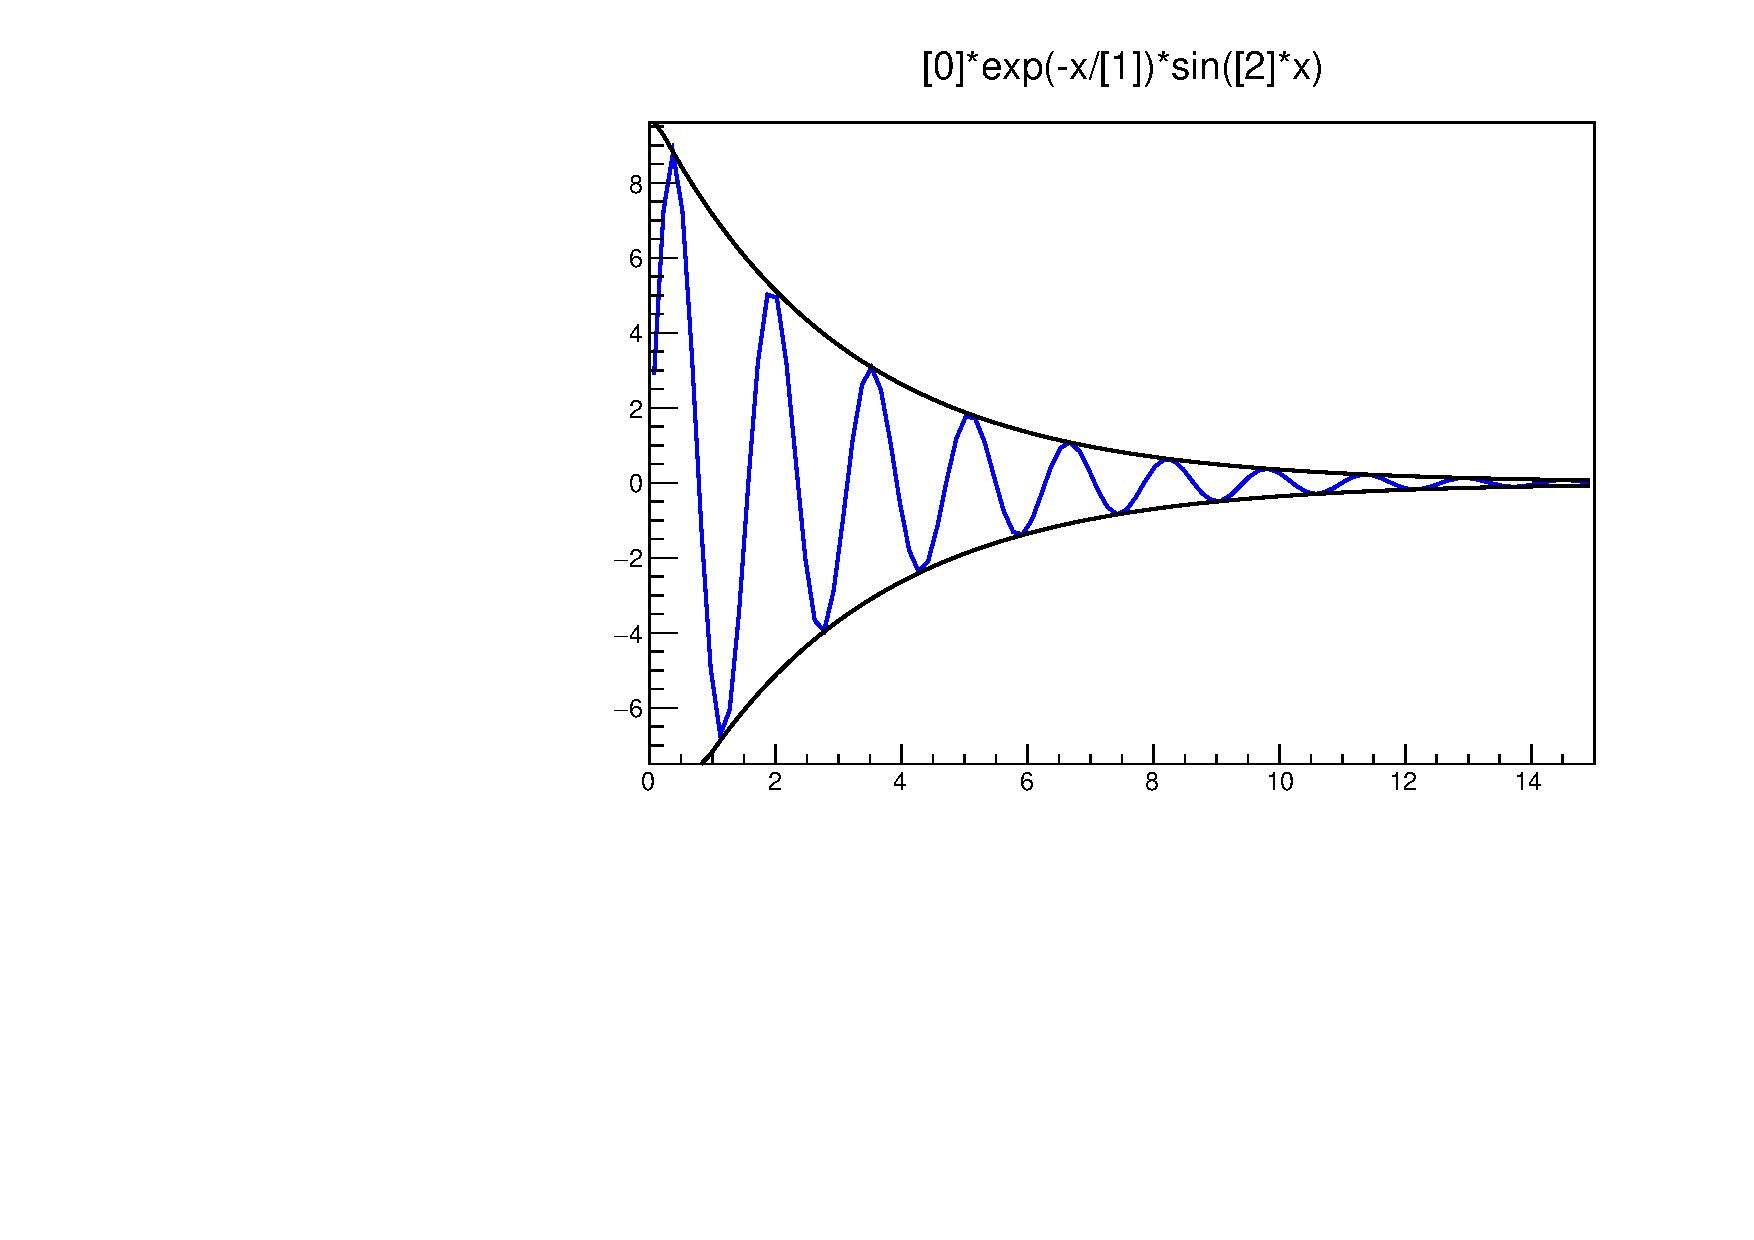
\includegraphics[scale=0.5]{funz.pdf}
\caption{Figura prodatta dallo script funzione.C.\label{funzi}}
\end{figure}


Proviamo a scrivere una funzione un po' più complicata, immaginiamo un fenomeno che obbedisca ad una legge della forma:

\begin{equation}
R_p=A\cdot\frac{\sqrt{1-(\frac{sin(\theta)}{n_1})^2}-n_1\cdot cos(\theta)}{\sqrt{1-(\frac{sin(\theta)}{n_1})^2}+n_1\cdot cos(\theta)} \label{rdip}
\end{equation}

scriviamo lo script capace di mettere a grafico la funzione:

\begin{verbatim}
{  //script funzione_complicata.C
  TF1 *ff=new TF1("ff","[0]*pow((sqrt(1-pow(sin(x)/[1],2))
                        -[1]*cos(x))/  (sqrt(1-pow(sin(x)/[1],2))
                        +[1]*cos(x)),2)",25*3.14/180,75*3.14/180);
  ff->SetParameter(0,2320);
  ff->SetParameter(1,1.6);
  ff->Draw();
  }
\end{verbatim}
Notiamo come passiamo i valori ai due parametri attraverso il metodo \textit{SetParameter} e la figura \ref{funzi2} prodotta dallo script. 
\begin{figure}
\centering
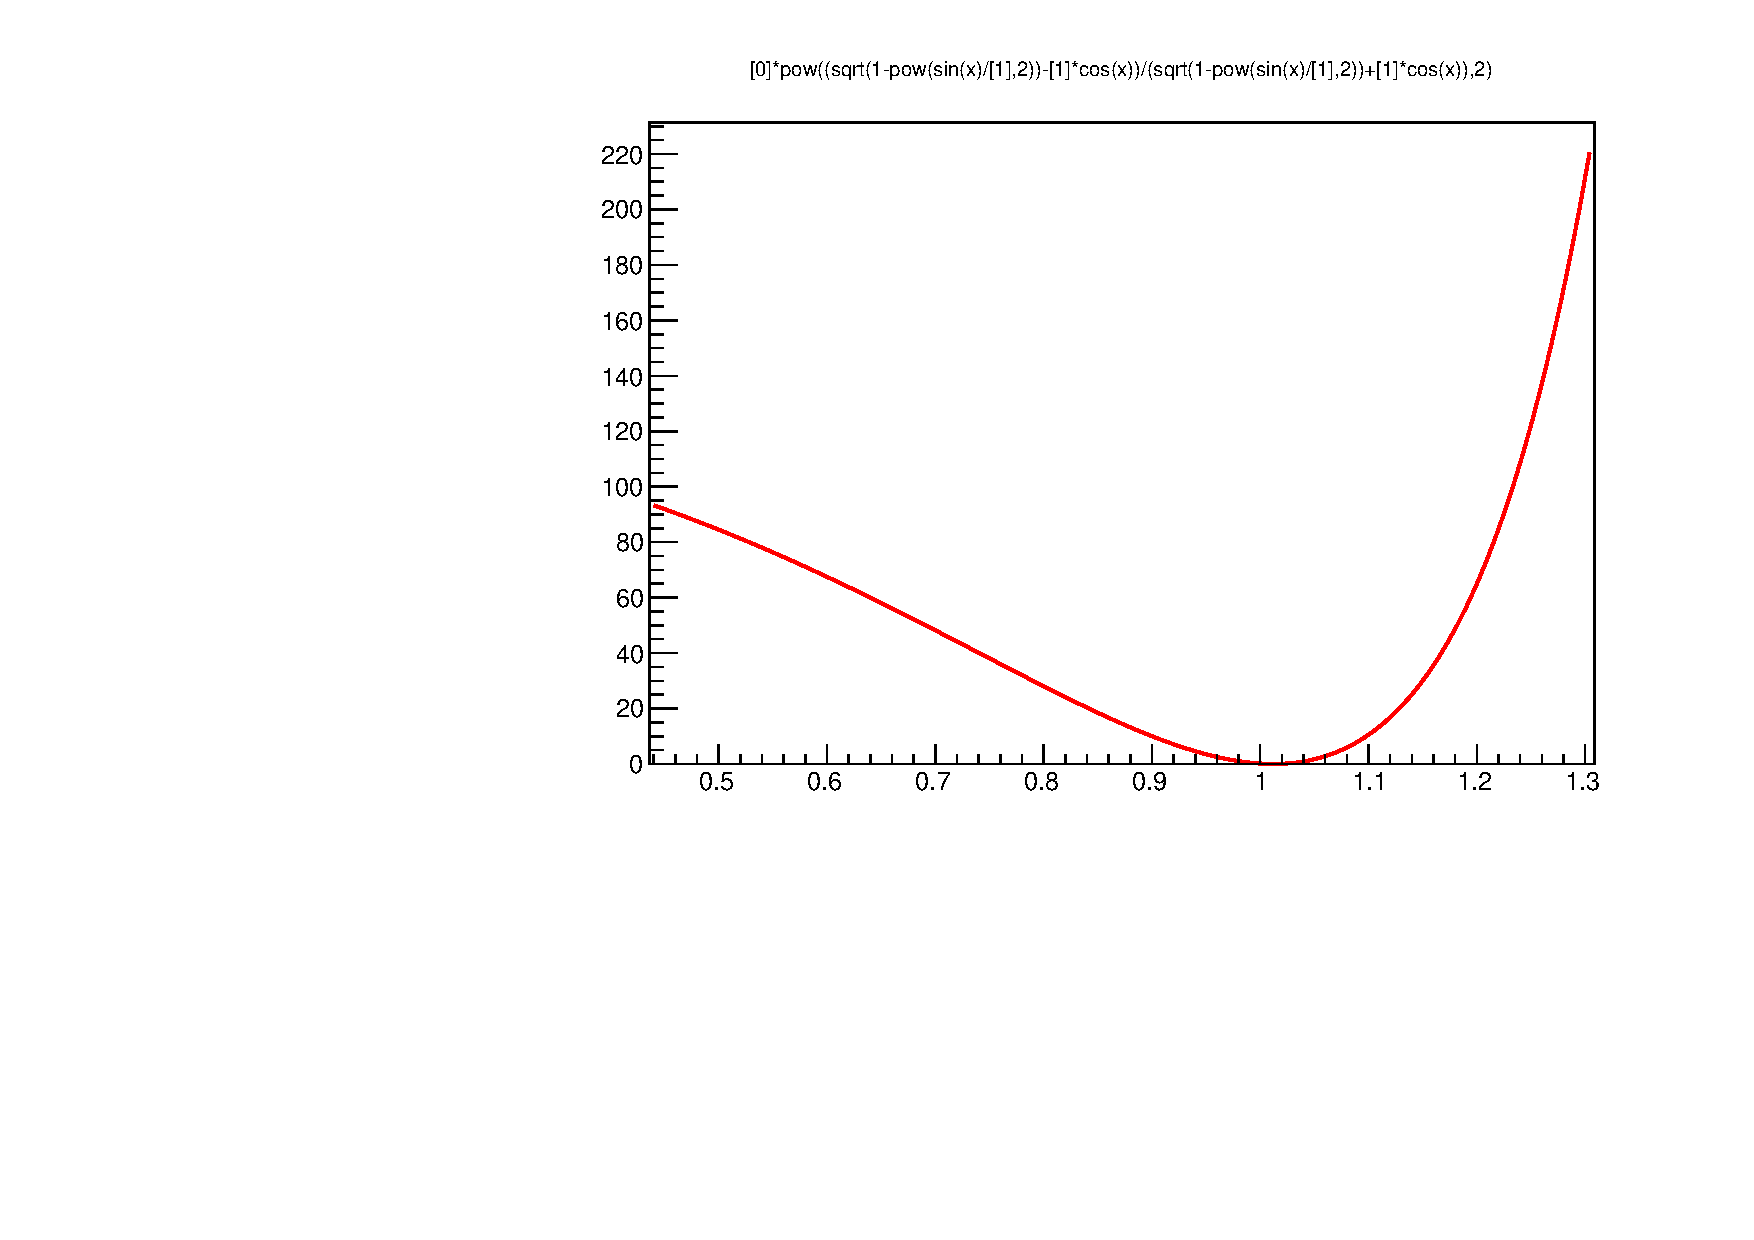
\includegraphics[scale=0.5]{funzcomp.pdf}
\caption{Figura prodatta dallo script funzione.C.\label{funzi2}}
\end{figure}

Non bisogna dimenticare che la programmazione è uno strumento per risolvere problemi e root fornisce un arsenale di possibilità per analizzare dati, ma tutto ciò che scriviamo deve obbedire alle regole della matematica e possibilmente avere anche senso dal punto di vista della fisica.
Se ad esempio assegnassimo al parametro $n_2$ dell'equazione \ref{rdip} il valore 0.5 cosa succederebbe? L'analisi ci dice che la funzione seno è limitata tra $\pm$1 quindi se $n_2<$1 può accadere che per certi valori di $\theta$ la funzione non ammetta valori reali. Proviamo a ``girare'' lo script assegnando il valore 0.5 ($ff->SetParameter(1,0.5);$), il risultato che vedremo è il seguente:
\begin{verbatim}
root [0] 
Processing funz2.C...
Info in <TCanvas::MakeDefCanvas>:  created default TCanvas with name c1
Warning in <TCanvas::ResizePad>: Inf/NaN propagated to the pad. 
Check drawn objects.
Warning in <TCanvas::ResizePad>: c1 height changed from 0 to 10

root [1] Warning in <TCanvas::ResizePad>: Inf/NaN propagated to the pad.
Check drawn objects.
Warning in <TCanvas::ResizePad>: c1 height changed from 0 to 10

Warning in <TCanvas::ResizePad>: Inf/NaN propagated to the pad. 
Check drawn objects.
Warning in <TCanvas::ResizePad>: c1 height changed from 0 to 10
\end{verbatim}
root produce dei messaggi di errore e li stampa a schermo, ma l'errore lo abbiamo commesso noi, non vuol dire che root non funziona anzi vuol dire il contrario.

%\section{Rappresentazione di dati}\index{Rappresentazione di dati}
\section{Fit}\index{Fit}

Il fit è una procedura matematica-numerica che consente di determinare i parametri (e l'incertezza con la quale vengono determinati) di una data legge (funzione) che noi assumiamo possa descrivere l'andamento di dati correlati. Se mettiamo un filo metallico in trazione con un peso e ne misuriamo la lunghezza, poi aggiungiamo un ulteriore peso e riusciamo ad apprezzare un aumento della lunghezza, ripetiamo l'operazione e ci annotiamo queste due grandezze, ad esempio potremmo supporre che trazione e allungamento siano legate da una legge di tipo lineare; lo stesso se sottoponiamo a riscaldamento una barra metallica; o che le oscillazioni di un pendolo obbediscano ad una legge come quella messa in grafico in figura \ref{funzione} etc. Finora abbiamo parlato di leggi di tipo fisico, ma la legge che descrive l'andamento dei dati potrebbe essere di tipo statistico. La distribuzione delle lunghezze dei chiodi fabbricati per lavori di carpenteria, le palline di plastica di cui abbiamo parlato nei paragrafi precedenti producono istogrammi con distribuzione di tipo gaussiano, quindi l'istogramma potrebbe essere fittato con una gaussiana. Quindi non solo leggi fisiche ma anche andamenti statistici.

root mette a disposizione una serie di funzione già implementate, di largo uso, per effettuare i fit oppure consente all'utente di scrivere da se la legge con la quale si vuole fare il fit attraverso una classe di tipo \textbf{TF1} e usarla in un calcolo completamente personalizzato.

Le funzioni preconfezionate di root sono la Gaussiana (parola chiave: \textbf{gaus}, Gaussiana con 3 parametri: $f(x) = p0\cdot exp(-0.5\cdot ((x-p1)/p2)^2))$, la Landau (\textbf{landau}, funzione a due parametri, valore medio e sigma), la funzione esponenziale (\textbf{expo}, funzione esponenziale con due parametri: $f(x) = exp(p0+p1\cdot x)$), i polinomi (\textbf{polN}, dove la N va sostituita con 0 se volete fare un fit con una costante, 1 per la retta, 2 parabola; insomma ci siamo capiti, N indica l'ordine del polinomio che desiderate usare).

Se volessimo fittare la distribuzione delle palline e dei chiodi presentate nelle figure \ref{menogrezzo} e \ref{chiodi} basterebbe usare il metodo \textbf{Fit} della classe \textbf{TH1F} passandogli l'opzione \textbf{gaus}.
\begin{verbatim}
pippo->Fit("gaus");
\end{verbatim}
e otterremmo il risultato riportato in figura \ref{fittini}. Ovviamente, ciò che stiamo riportando è a titolo di esempio e serve a rompere il ghiaccio con questi metodi. Il metodo Fit possiede molte opzioni che vi consentiranno di studiare i vostri dati in modo molto più sofisticato (\textit{https://root.cern.ch/root/html534/guides/users-guide/FittingHistograms.html\#the-fit-method}).

\begin{figure}
\centering
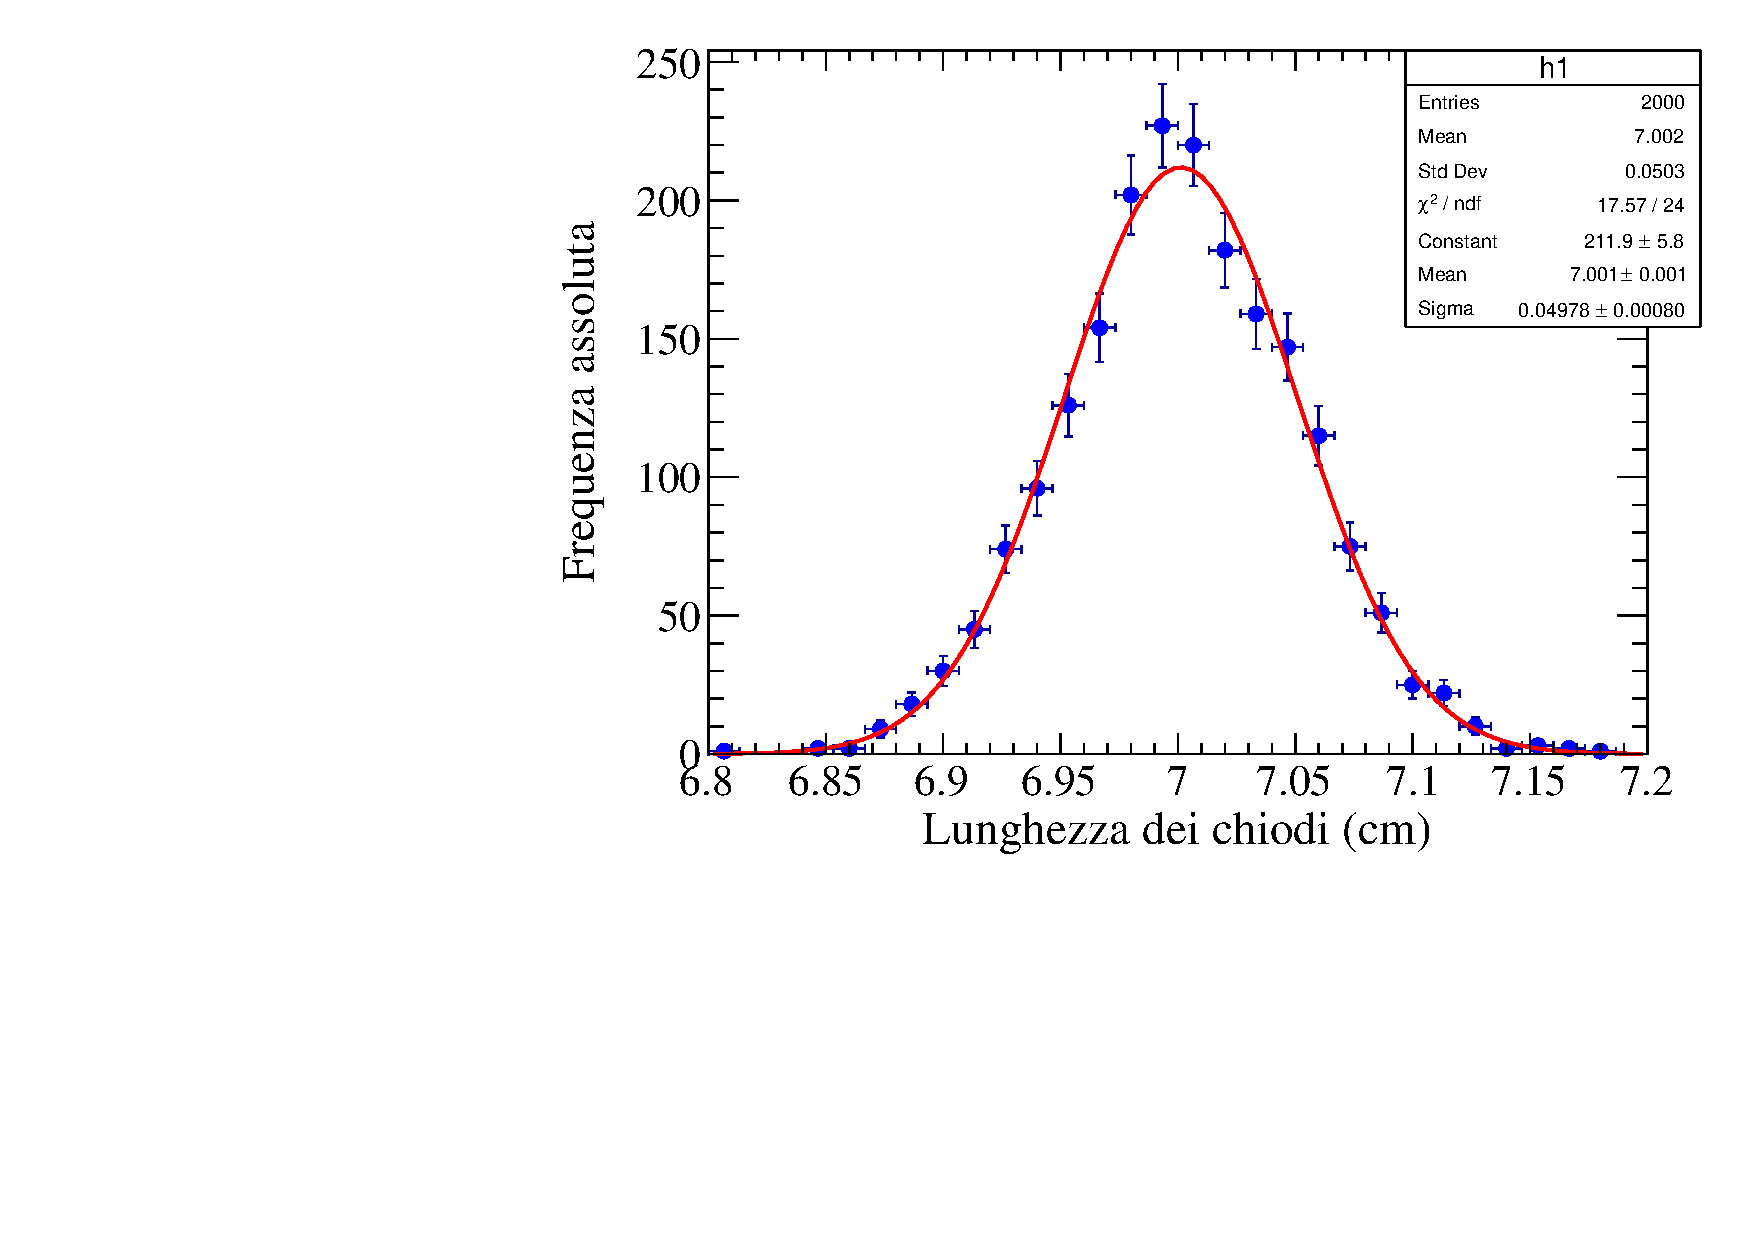
\includegraphics[scale=0.35]{chiodiistpf.pdf}
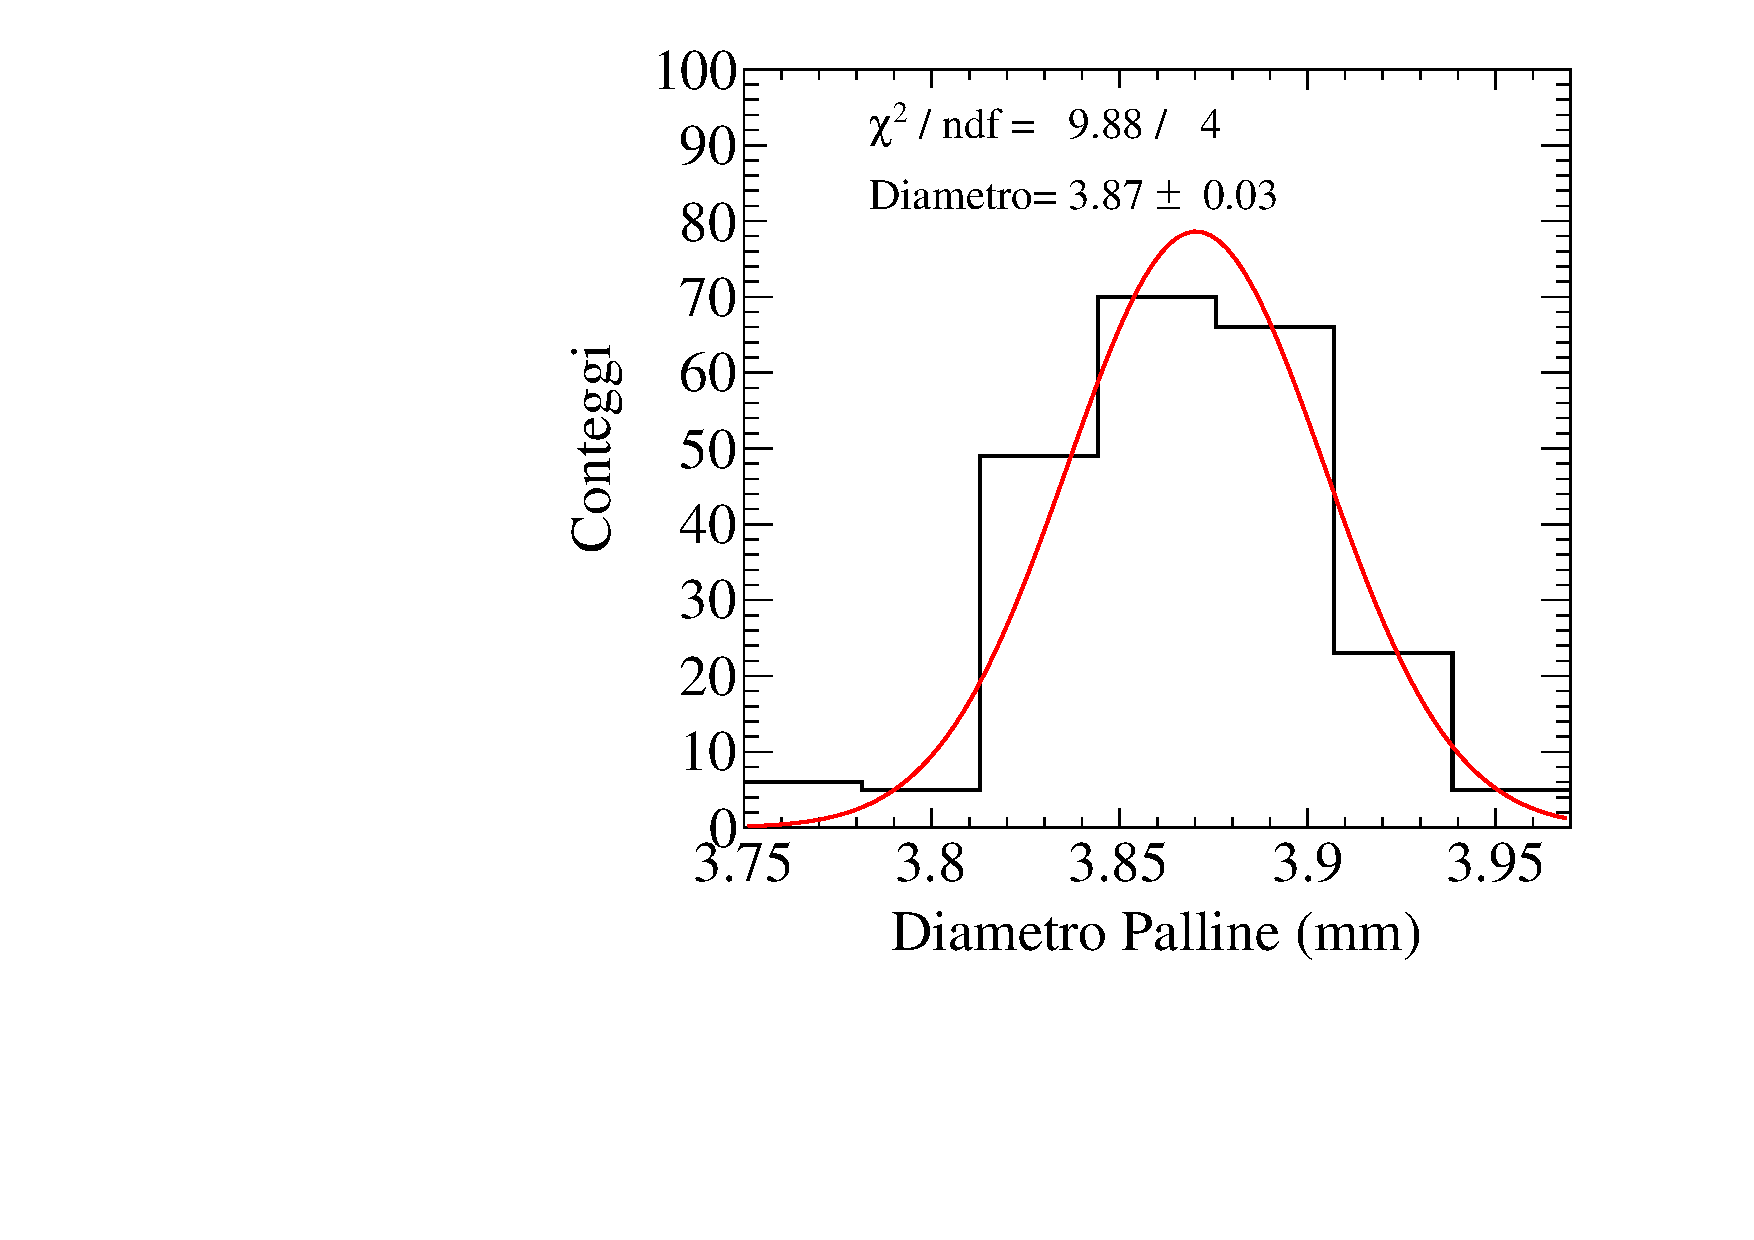
\includegraphics[scale=0.35]{pallinefit.pdf}
\caption{  .\label{fittini}}
\end{figure}

La distribuzione è chiare negli esempi appena esposti, e invocando direttamente il metodo di fit abbiamo buone possibilità di ottenere il risultato desiderato. In generale quando si effettuano delle operazioni di fit al calcolatore, gli algoritmi di ricerca dei parametri hanno bisogno di un suggerimento, hanno bisogno che gli diamo dei valori vicini a quelli attesi per poi delegare loro alla ricerca dei migliori valori, migliori nel senso quelli che producono la curva che più si avvicina ai dati.
I dati suggeriti al fit vengono chiamati parametri di innesco del fit.
Uno dei metodi per stabilire la bontà di un fit è quello del $\chi^2$.
La variabile del $\chi^2$ si costruisce come la sommatoria degli scarti quadratici tra i valori sperimentali e quelli del fit normalizzati al quadrato della somma  dei rispettivi errori (errore sperimentale ed indeterminazione della funzione di fit). Ricercare i valori dei parametri della funzione che rendono minima questa variabile può rappresentare un criterio per la ricerca del fit migliore (il best fit).

Supponiamo ora di aver effettuato un esperimento che mette in relazione  l'angolo rispetto al quale un foto-rivelatore misura un segnale e la misura stessa del segnale espressa in Millivolt (mV). I dati in questione sono scritti nel file \textit{datuzzi.dat} e in Tabella \ref{datuzzi}.

\begin{table}[h]
\centering
\caption{Tabella dei dati scritti nel file datuzzi.dat.\label{datuzzi}}
\vspace{0.2cm}
\begin{tabular}{c|c}
$\theta_i$ (rad.) & R$_p$ (mV)\\
\hline
0.441868 & 79.10\\
\hline
0.616312 & 53.20\\
\hline
0.790757 & 18.70\\
\hline
0.860534 & 9.16\\
\hline
0.965201 & 2.00\\
\hline
1.03498 & 7.60\\
\hline
1.06987 & 13.70\\
\hline
1.13965 & 43.45\\
\hline
1.20942 & 101.50\\
\hline
1.31409 & 249.20
\end{tabular}
\end{table}

Ora supponiamo che la legge definita dalla funzione \ref{rdip} sia quella che regola la relazione tra le due grandezze appena misurate e proviamo quindi ad usarla per implementare un fit. Lo script che segue è completo di tutti i ghirigori necessari per ottenere una figura decorosa, ma in realtà le uniche istruzioni necessarie per portare ``a casa'' il fit sono segnate nel codice sorgente con tre asterischi.

\begin{verbatim}
//codice con fit su dati senza attribuire l'errore
// Script fitnoerr
{
  int mymarkerstyle=20;
  float mymarkersize=1.;
  float mytextsize=0.065;
  int mytextfont=132;
  TCanvas *Canvas_1 = new TCanvas("Canvas_1", "Canvas_1",600,500);
  Canvas_1->SetFillColor(0);
  Canvas_1->SetBorderMode(0);
  Canvas_1->SetBorderSize(2);
  Canvas_1->SetLeftMargin(0.15);
  Canvas_1->SetRightMargin(0.07);
  Canvas_1->SetTopMargin(0.03);
  Canvas_1->SetBottomMargin(0.16);
 //  Canvas_1->SetGridx();
 //  Canvas_1->SetGridy();
  Canvas_1->SetTickx(1);
  gStyle->SetOptStat(1111);
  TF1 *ff=new TF1("ff","[0]*pow((sqrt(1-pow(sin(x)/[1],2))
                        -[1]*cos(x))/  (sqrt(1-pow(sin(x)/[1],2))
                        +[1]*cos(x)),2)",25*3.14/180,75*3.14/180);//***
  //parametri di innesco
  ff->SetParameter(0,2320);//***
  ff->SetParameter(1,1.6);//***
  TGraph *pippo= new TGraph("datuzzi.dat");//**
  pippo->SetTitle("");
  pippo->GetXaxis()->SetTitleSize(mytextsize);
  pippo->GetYaxis()->SetTitleSize(mytextsize);
  pippo->GetXaxis()->SetLabelSize(mytextsize);
  pippo->GetYaxis()->SetLabelSize(mytextsize);
  pippo->GetXaxis()->SetTitleFont(mytextfont);
  pippo->GetYaxis()->SetTitleFont(mytextfont);
  pippo->GetYaxis()->CenterTitle(1);
  pippo->GetXaxis()->CenterTitle(1);
  pippo->GetYaxis()->SetTitleOffset(1.1);
  pippo->GetXaxis()->SetTitleOffset(1.10);
  pippo->GetYaxis()->SetTitle("R_{p} (mV)");
  pippo->GetXaxis()->SetTitle("#theta_{i} (rad.)");
  pippo->SetMarkerStyle(20);
  pippo->Draw("ap");
  pippo->Fit("ff");//***
  float media,sigma,media2,sigma2,chi,ndf;
  TLegend *leg = new TLegend(0.2,0.7,0.55,0.85,NULL,"brNDC");
  leg->SetBorderSize(0);
  leg->SetLineColor(1);
  leg->SetLineStyle(1);
  leg->SetLineWidth(1);
  leg->SetFillColor(0);
  leg->SetTextSize(0.05);
  leg->SetTextFont(132);
  leg->SetFillStyle(1001);
  media=ff->GetParameter(0);
  sigma=ff->GetParError(0);
  media2=ff->GetParameter(1);
  sigma2=ff->GetParError(1);
  chi=ff->GetChisquare();
  ndf=ff->GetNDF();
  leg->AddEntry(pippo,Form("#chi^{2} / ndf = %6.2f / %3.0f",chi,ndf),"");
  leg->AddEntry(pippo,Form("A=%5.2f #pm %5.2f",media,sigma),"");
  leg->AddEntry(pippo,Form("n2=%5.2f #pm %5.2f",media2,sigma2),"");
  leg->Draw();
  Canvas_1->SaveAs("fit.pdf");
}
\end{verbatim}

Il fit riportato in figura \ref{fitnoerr} appare buono, la curva è molto vicina ai punti sperimentali e i parametri ragionevoli per la fisica che regola questo fenomeno, tuttavia la variabile del $\chi^2$ è grande e questo in generale vuol dire che il fit non è buono. Come interpretare questo risultato?
\begin{figure}[h]
\centering
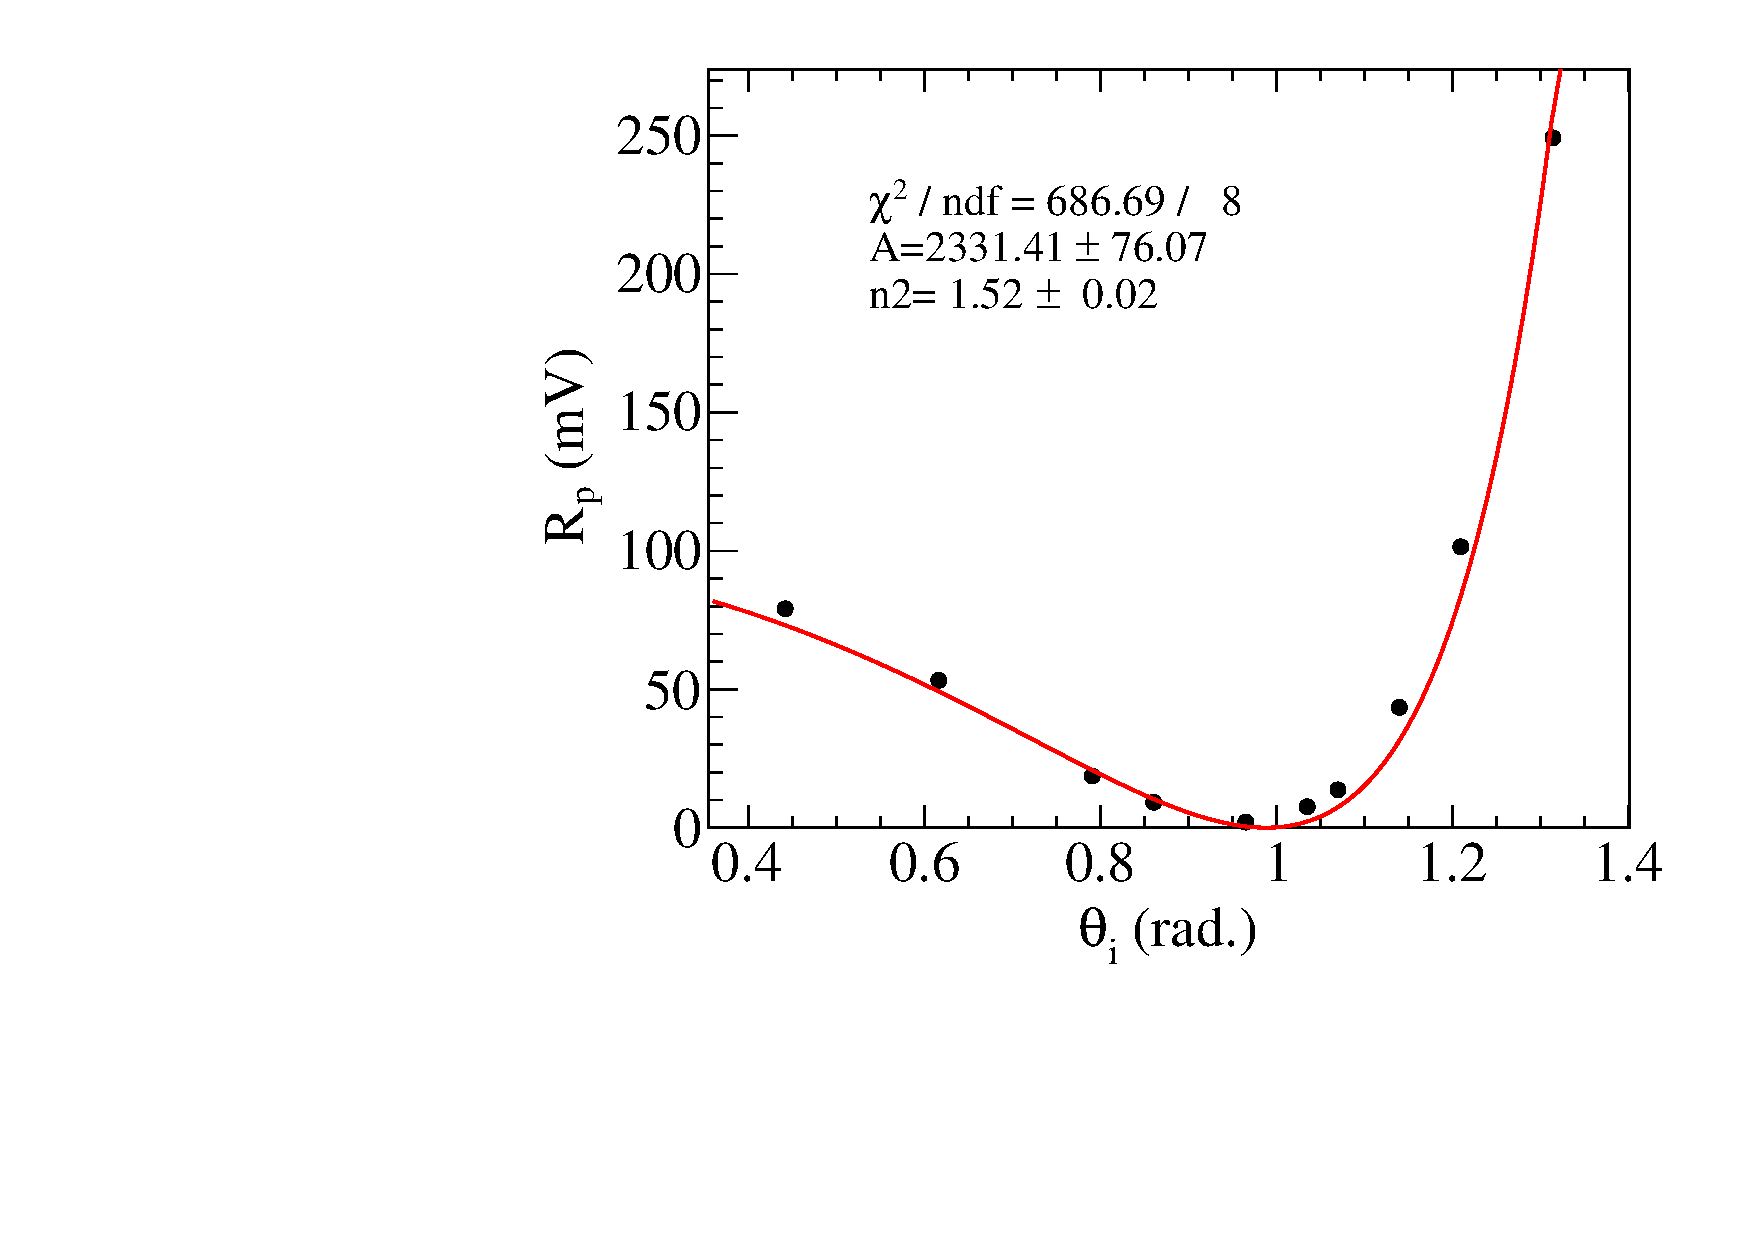
\includegraphics[scale=0.5]{fit.pdf}
\caption{Risultato dello script Script fitnoerr. \label{fitnoerr}}
\end{figure}

In realtà la nostra percezione è corretta, il fit è realmente buono, ma è anche vero che il $\chi^2$ è stato calcolato correttamente. Il motivo dell'apparente discordanza è legato fatto che non abbiamo associato ai valori sperimentali i relativi errori. In tabella \ref{datuzzierr} riportiamo i dati in questione, ma questa volta riportiamo anche gli errori sperimentali: quelli relativi all'angolo e quelli relativi all'intensità del foto-rivelatore.

\begin{table}
\centering
\caption{Tabella dei dati scritti nel file datuzzierr.dat.\label{datuzzierr}}
\vspace{0.3cm}
\begin{tabular}{c|c|c|c}
$\theta_i$ (rad.) & R$_p$ (mV)& err. $\theta_i$ (rad.) & err.   R$_p$ (mV)\\
\hline
0.441868 & 79.10 &   0.0349067  &  5\\
\hline
0.616312 & 53.20 &   0.0349067  &  5\\
\hline
0.790757 & 18.70  &   0.0349067  &  5\\
\hline
0.860534 & 9.16 &   0.0349067  &  5\\
\hline
0.965201 & 2.00 &   0.0349067  &  5\\
\hline
1.03498 & 7.60 &   0.0349067  &  5\\
\hline
1.06987 & 13.70 &   0.0349067  &  5\\
\hline
1.13965 & 43.45 &   0.0349067  &  5\\
\hline
1.20942 & 101.50 &   0.0349067  &  5\\
\hline
1.31409 & 249.20  &   0.0349067  &  5
\end{tabular}
\end{table}

Rifacciamo il fit e modifichiamo lo script utilizzato in precedenza facendo una variazione piccolissima nel codice: passiamo dalla classe \textbf{TGraph} alla classe \textbf{TGraphErrors} che consente di tenere in conto anche degli errori sulle variabili ascissa e ordinata.

\begin{verbatim}
// script fitsierr.C
//tutto come nella macro precedente
//cambia solo la classe che si preoccupa
//di caricare e rappresentare i dati
//passiamo da TGraph a TGraphErrors
.....
.....
TGraphErrors *pippo= new TGraphErrors("datuzzierr.dat");
.....
 Canvas_1->SaveAs("fiterr.pdf");
\end{verbatim}

Il risultato di questo secondo fit è leggermente differente dal precedente, ma in perfetto accordo nei limiti degli errori sul parametri che volevamo determinare, mentre il $\chi^2$ è decisamente piccolo e in accordo con la nostra percezione della bontà del fit. In questo secondo fit, il calcolatore ha tenuto conto anche dell'errore sperimentale, mentre nel primo fit non avendo incluso questa informazione ha normalizzato gli scarti, fattori del calcolo della variabile statistica $\chi^2$, al solo errore commesso nel fit.


\begin{figure}[h]
\centering
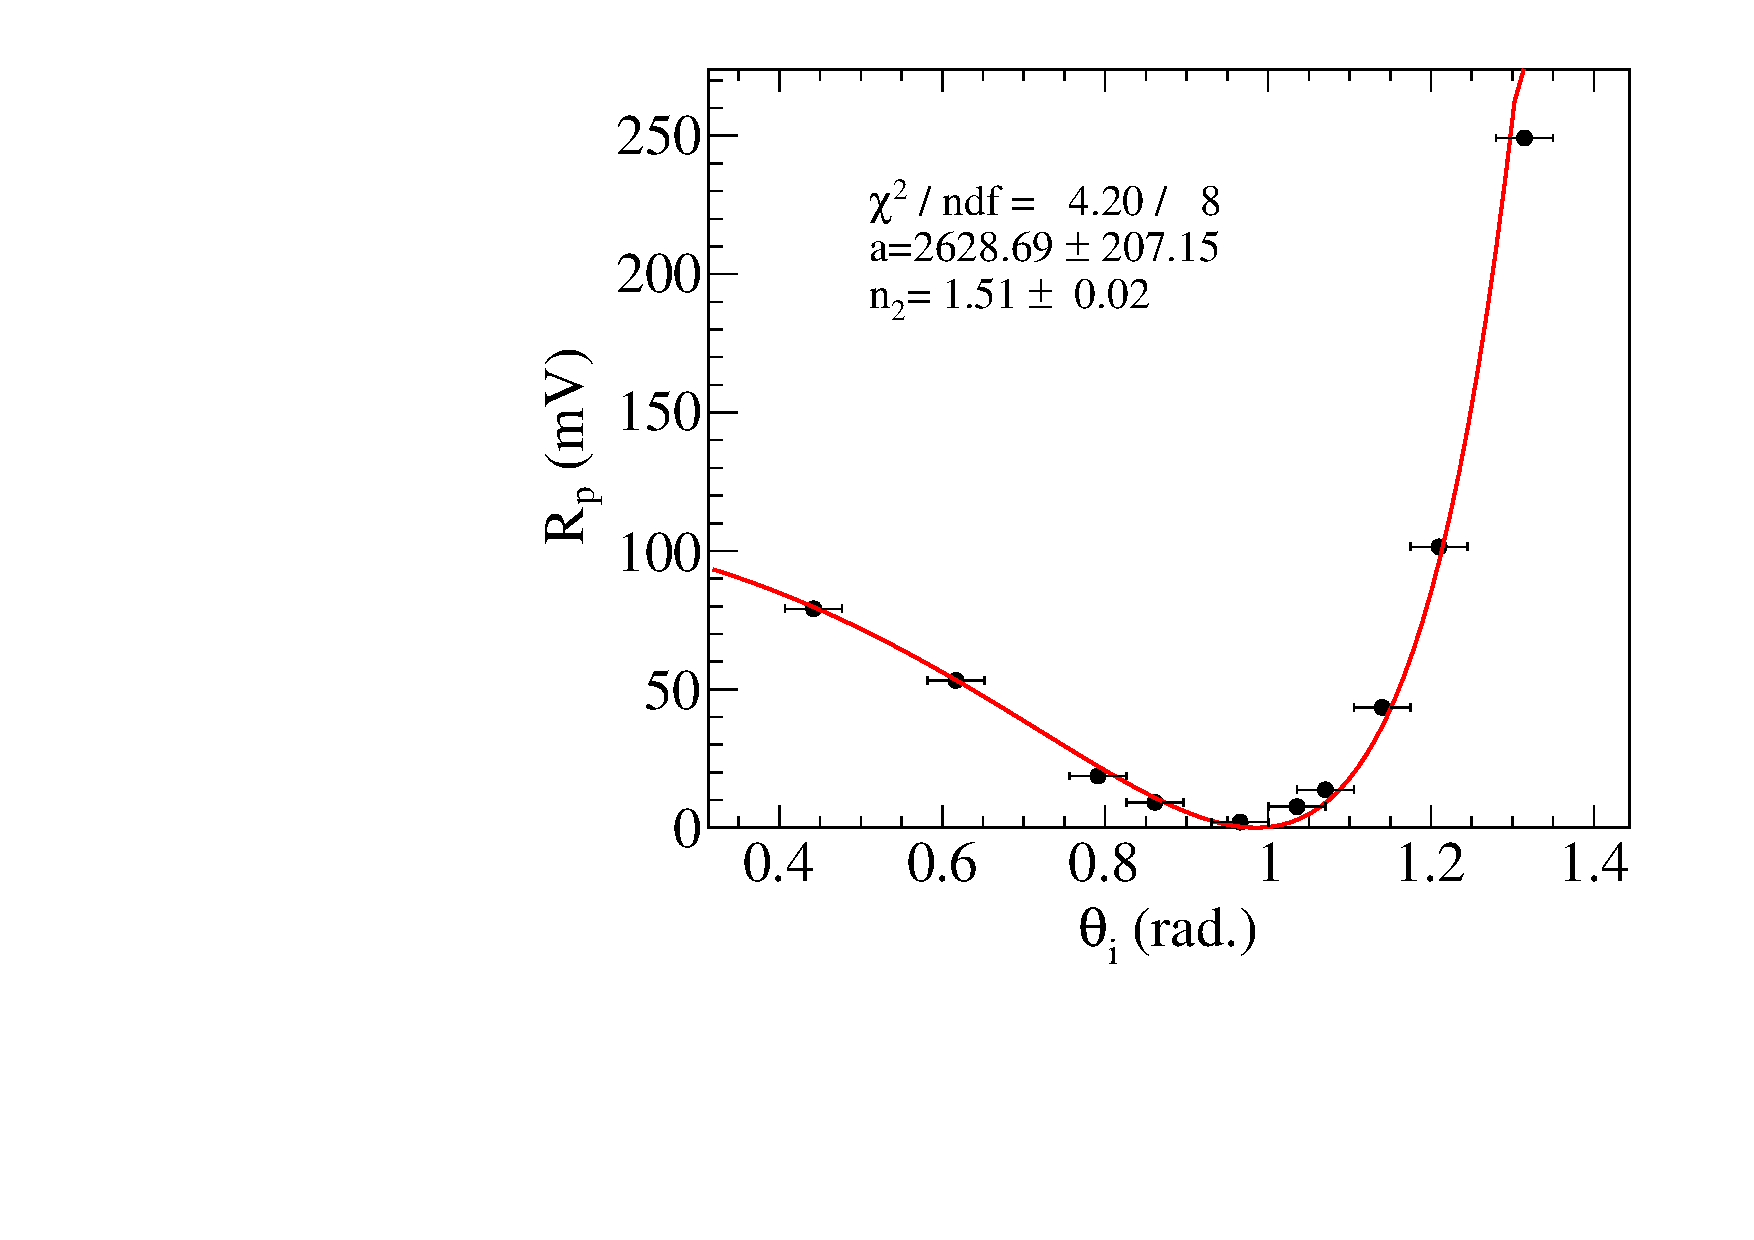
\includegraphics[scale=0.5]{fiterr.pdf}
\caption{Risultato dello script Script fitsierr. \label{fiterr}}
\end{figure}
Spieghiamo meglio questa questione, il fit (la curva rossa nelle figure di questo paragrafo) ha un errore associato, non è priva da errore. Se notate in figura i parametri $A$ e $n_2$ hanno una indeterminazione. Ebbene se propaghiamo gli errori associati ai parametri nella formula descritta dalla funzione \ref{rdip} otteniamo l'errore associato al fit.
\newpage
\section{Macro intersezione}\index{Macro intersezione}

Questo esempio illustra un metodo per estrarre le intersezioni tra due funzioni nel piano, utilizzando le classi TF1 di root e la potentissima classe Vector di C++. I commenti a corredo del codice


\begin{verbatim}
{
//la classe vector di c++ ci consente di creare vettori dinamici
//che si accrescono a nostro piacimento e i cui elementi
//all'occorrenza possono essere eliminati senza incorrere in errori
//di segmentazione
vector<double> low ;
vector<double> high ;

TF1 * par = new TF1("par","sin(x)",0,20);
TF1 * ret = new TF1("ret","-x/20",0,20);
TF1 * diff = new TF1("diff","par-ret",0,20);

diff->Draw();
int numdiv = 1000000;
double passo = 20./double(numdiv);
double ipsilon;
double spia = 1;
double x=0;
ipsilon=diff->Eval(x);
if(ipsilon<0)
{
spia=-1;
}
if(ipsilon==0)
{
ipsilon=diff->Eval(x+passo);
if(ipsilon<0)spia=-1;
}
for(int i=0; i<numdiv; i++){
x=x+passo;
//x= x + passo;
//
ipsilon=diff->Eval(x);
if(spia*ipsilon<0){
cout<<double(i-1)*passo<<"   "<<double(i)*passo<<endl;
//uso i vettori dinamici per copiare gli estremi inferiori
//e superiori di tutte le possibili interserzioni
low.push_back(double(i-1)*passo);
high.push_back(double(i)*passo);
spia=-spia;
}
}

//creo un vettore di puntatori a TF1
vector<TF1*> funzy;
//array di caratteri 
char nome[20];

//questa classe di c++, vi consente
//di usare un oggetto come se fosse un cin e cout
//contemporaneamente agendo su stringhe di caratteri
//utile per creare stringhe in modo dinamico
stringstream ss;

for(int i=0; i<low.size(); i++)
{
//ss carica la parola zero con un numero i che si modifica dinamicamente con il ciclo
ss<<"zero"<<i;
//ss scarica il suo contenuto nella variabile nome
ss>>nome;
//creiamo un indirizzo a oggetto TF1 e lo mettiamo in funzy
funzy.push_back(new TF1(nome,"fabs(par-ret)",low.at(i),high.at(i)));
//cancelliamo il contenuto dell'oggetto ss per usarlo vuoto al prossimo giro.
ss.clear();
//stampiamo le intersezioni!!!
cout<<"ecco l'intersezione x"<<i<<"  "<<funzy.at(i)->GetX(funzy.at(i)->GetMinimum())<<endl;
}
ret->SetLineColor(4);

par->Draw();
ret->Draw("same");

c1->SaveAs("duefunzioni.pdf");

diff->SetLineColor(1);

diff->Draw();

c1->SaveAs("diffe.pdf");



}

\end{verbatim}


\chapter{Rappresentazione dati tramite istogrammi}\index{Rappresentazione dati tramite istogrammi}

Quando si ha a che fare con misure ripetute o dati numerici acquisiti nelle medesime condizioni, uno dei modi più comodi per rappresentarli e analizzarli è quello dell'istogramma. Gli istogrammi possono essere monodimensionali o multidimensionali. La loro computazione è piuttosto semplice, è sufficiente determinare il massimo e il minimo assoluti della data distribuzione in esame, e poi suddividere tale intervallo in un certo numero arbitrario di sotto intervalli (bin), dopo di che si ripassano in rassegna tutti i dati e si conta il numero di volte che i dati sono caduti all'interno di un dato sottointervallo. Il numero di volte che le misure cadono in un bin è la frequenza assoluta.
A questo punto per rappresentare l'istogramma è sufficiente porre sull'asse x la variabilità della misura e indicare tutti i sottointervalli, e sull'asse y la frequenza assoluta di ciascun intervallo. 

In questo capitolo studieremo le classi di ROOT, THD, che forniscono molteplici strumenti per analizzare i dati tramite gli istogrammi.



\section{Il mio primo istogramma con ROOT}\index{Il mio primo istogramma con ROOT}

%Per evitare ripetizioni su cosa sia ROOT, rimandiamo il lettore alla referenza \cite{appunti:1}, ultimi due capitoli.

Per poter costruire un istogramma, come primo ingrediente abbiamo bisogno dei dati, e supponiamo che questi siano stati copiati in un file ``dati1x.dat'' scritti su di una sola colonna, o su una sola riga, o disordinatamente, nel nostro caso è ininfluente.
Il modo più semplice per computare un istogramma con ROOT è quello di scrivere una macro capace di leggere i dati, fornirli a un oggetto della classe TH1D, e poi utilizzare il metodo Draw per visualizzare il risultato. Il codice di che opera quanto detto è riportato di seguito.

\begin{lstlisting}[language=c++]
{//inizio della macro
ifstream leggo("dati1x.dat");
if(leggo.fail())
    {
    cout<<"the file does not exist!"<<endl;
    }
double a;
//dichiarazione oggetto della classe TH1D
TH1D *hist = new TH1D("hist","",50,0,0);
while(leggo>>a)
    {
    hist->Fill(a);  
    }
hist->Draw();
}//fine della macro
\end{lstlisting}

\begin{figure}
\centering
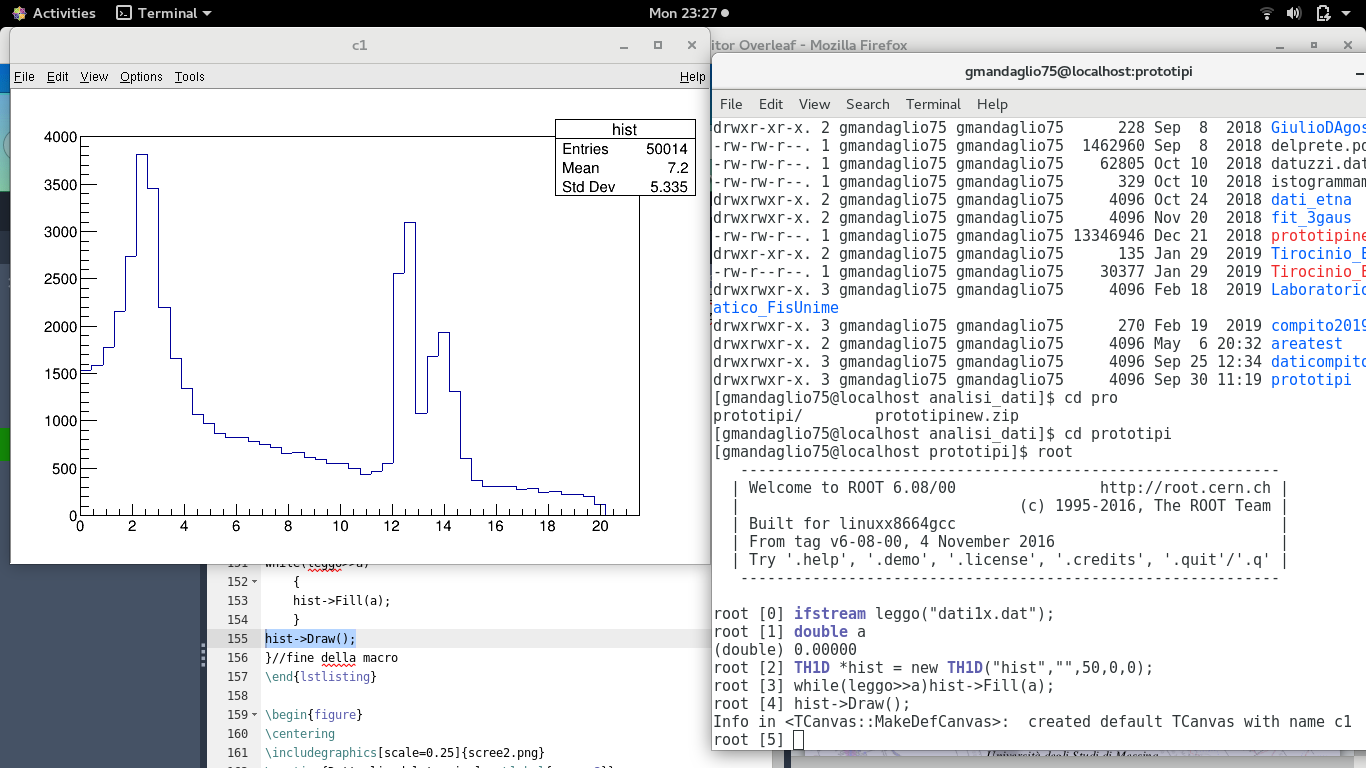
\includegraphics[scale=0.25]{Pictures/screen1.png}
\caption{Dettaglio dei comandi presenti nella macro che legge i dati e computa l'istogramma. \label{screen1}}
\end{figure}


In Figura  \ref{screen1} è mostrato il risultato dei comandi della macro. Come si può notare ROOT ha aperto una interfaccia grafica, che si chiama canvas, nella quale ha immagazzinato l'immagine contente l'istogramma. Per default la canvas creata da ROOT si chiama c1, più avanti vederemo che abbiamo pieno controllo delle canvas e che queste vengono guidate attraverso la classe TCanvas. 
Se volessimo salvare la figura prodotta in un formato da riutilizzare per un articolo, una relazione, una presentazione, è sufficiente utilizzare il metodo SaveAs della Canvas, come di seguito

\begin{lstlisting}[language=c++]
{//inizio della macro
.....
hist->Draw();
c1->SaveAs("ilmiografico.pdf");//l'estensione del file dice a ROOT in che formato salvare la figura
}//fine della macro
\end{lstlisting}


\section{I miei primi 10 istogrammi}\index{I miei primi 10 istogrammi}
Immaginiamo ora di avere a che fare con un file di dati contenete 10 colonne di numeri, e che ogni colonna sia composti da dati provenienti da una misura ripetuta, da un simulatore o altro; e immaginiamo di voler utilizzare il codice appena studiato per produrre l'istogramma della colonna n. 3.
Il modo più grezzo per farlo è quello di sfruttare il metodo di lettura dell'oggetto ifstream e leggere direttamente una riga per volta.

\begin{lstlisting}[language=c++]
{//inizio della macro
ifstream leggo("dati1x.dat");
if(leggo.fail())
    {
    cout<<"the file does not exist!"<<endl;
    }
double a1,a2,a3,a4,a5,a6,a7,a8,a9,a10;
//dichiarazione oggetto della classe TH1D
TH1D *hist = new TH1D("hist","",50,0,0);
while(leggo>>a1>>a2>>a3>>a4>>a5>>a6>>a7>>a8>>a9>>a10)//leggo una riga per volta
    {
    hist->Fill(a3); //passo solo il valore della terza colonna  
    }
hist->Draw();
}//fine della macro
\end{lstlisting}

La macro funziona, ma siamo riusciti a uscirne vivi perchè il numero delle colonne in questo caso è limitato. Questo ci fa capire che se anche la via più semplice sembra la più veloce non è detto che lo sia veramente o che sia la più conveniente a lungo termine.

Passando dalla filosofia alla pratica, mostriamo un modo leggermente più smart per risolvere lo stesso problema:

\begin{lstlisting}[language=c++]
{//inizio della macro
ifstream leggo("datoni.dat");
if(leggo.fail())
    {
    cout<<"the file does not exist!"<<endl;
    }
double a;
//dichiarazione oggetto della classe TH1D
TH1D *hist = new TH1D("hist","",50,0,0);
int contami =0;
while(leggo>>a)
    {
    contami++;//conta le letture effettuate
    if(contami==3){ //il numero nell'uguaglianza decide la colonna
        hist->Fill(a); //passo solo il valore della terza colonna
        }
        if(contami==10){
             contami=0;//azzero il contatore
            }
    }
hist->Draw();
}//fine della macro
\end{lstlisting}

Con un semplice sistema di contatori il codice è capace di sintonizzarsi sempre sulla medesima colonna.

Immaginiamo ora di voler creare direttamente 10 istogrammi, utilizzando sempre una variante dei codici appena scritti. Come procederemmo?
Una possibile soluzione, che funziona e che è abbastanza orribile, potrebbe essere quella di prenotare 10 istogrammi e....mi sento male a scriverlo...ma facciamo questo sacrificio:

\begin{lstlisting}[language=c++]
{//inizio della macro
ifstream leggo("datoni.dat");
if(leggo.fail())
    {
    cout<<"the file does not exist!"<<endl;
    }
double a;
//dichiarazione oggetto della classe TH1D
TH1D *h1 = new TH1D("h1","",50,0,0);
TH1D *h2 = new TH1D("h2","",50,0,0);
TH1D *h3 = new TH1D("h3","",50,0,0);
TH1D *h4 = new TH1D("h4","",50,0,0);
TH1D *h5 = new TH1D("h5","",50,0,0);
TH1D *h6 = new TH1D("h6","",50,0,0);
TH1D *h7 = new TH1D("h7","",50,0,0);
TH1D *h8 = new TH1D("h8","",50,0,0);
TH1D *h9 = new TH1D("h9","",50,0,0);
TH1D *h10 = new TH1D("h10","",50,0,0);

int contami =0;
while(leggo>>a)
    {
    contami++;//conta le letture effettuate
    if(contami==1){ 
        h1->Fill(a);
        }
    if(contami==2){ 
        h2->Fill(a);
        }
    if(contami==3){ 
        h3->Fill(a);
        }
    if(contami==4){ 
        h4->Fill(a);
        }
    if(contami==5){ 
        h5->Fill(a);
        }
    if(contami==6){ 
        h6->Fill(a);
        }
    if(contami==7){ 
        h7->Fill(a);
        }
    if(contami==8){ 
        h8->Fill(a);
        }
    if(contami==9){ 
        h9->Fill(a);
        }
    if(contami==10){ 
        h10->Fill(a);
        contami=0;
        }
    }
h1->Draw();
}//fine della macro
\end{lstlisting}

Per fare una cosa molto semplice abbiamo speso una pagina di appunti, questo ci fa capire che c'è un problema, e quindi ci ricordiamo che qualunque cosa che si ripete può essere agilmente risolta ricorrendo a un ciclo:

\begin{lstlisting}[language=c++]
{//inizio della macro
ifstream leggo("datoni.dat");
if(leggo.fail())
    {
    cout<<"the file does not exist!"<<endl;
    }
double a;
//dichiarazione oggetto della classe TH1D
TH1D *hist[10];
for(int i=1; i<11;i++){
 hist[i-1]= new TH1D(Form("h%d",i),"",50,0,0);
}
int contami =0;
while(leggo>>a)
    {
    contami++;//conta le letture effettuate
    if(a<10){
              hist[contami-1]->Fill(a);//ogni istogramma  viene riempito dalla c
orretta colonna
             }
        if(contami==10){
             contami=0;//azzero il contatore
            }
    }
hist[3]->Draw(); //disegno il grafico 4
}//fine della macro

\end{lstlisting}
Come possiamo notare il codice presenta un numero ridotto di righe, e soprattutto gode della proprietà di essere facilmente scalabile, in altre parole con piccolissime modifiche e senza aumentare le dimensioni del codice sarebbe capace di fare lo stesso lavoro per un numero grande a piacere di colonne (purtroppo risparmiamo solo codice, il costo computazionale cresce al crescere delle colonne che vogliamo leggere).

Nel codice che segue facciamo vedere come sia possibile utilizzare la TCanvas per immagazzinare tutti gli istogrammi prodotti aggiungendo qualche riga di codice a quello precedente:

\begin{lstlisting}[language=c++]
{//inizio della macro
.....
hist[3]->Draw(); //disegno il grafico 4
//parte in aggiunta alla macro precedente

TCanvas *scatolone = new TCanvas("scatolone","",800,400);
scatolone->Divide(5,2);

for(int i=0; i<10;i++){
 scatolone->cd(i+1);
 hist[i]->Draw();
}
//per salvare in un file le figure:
scatolone->SaveAs("10histo.pdf");
}//fine della macro
\end{lstlisting}


\begin{figure}[htb]
\centering
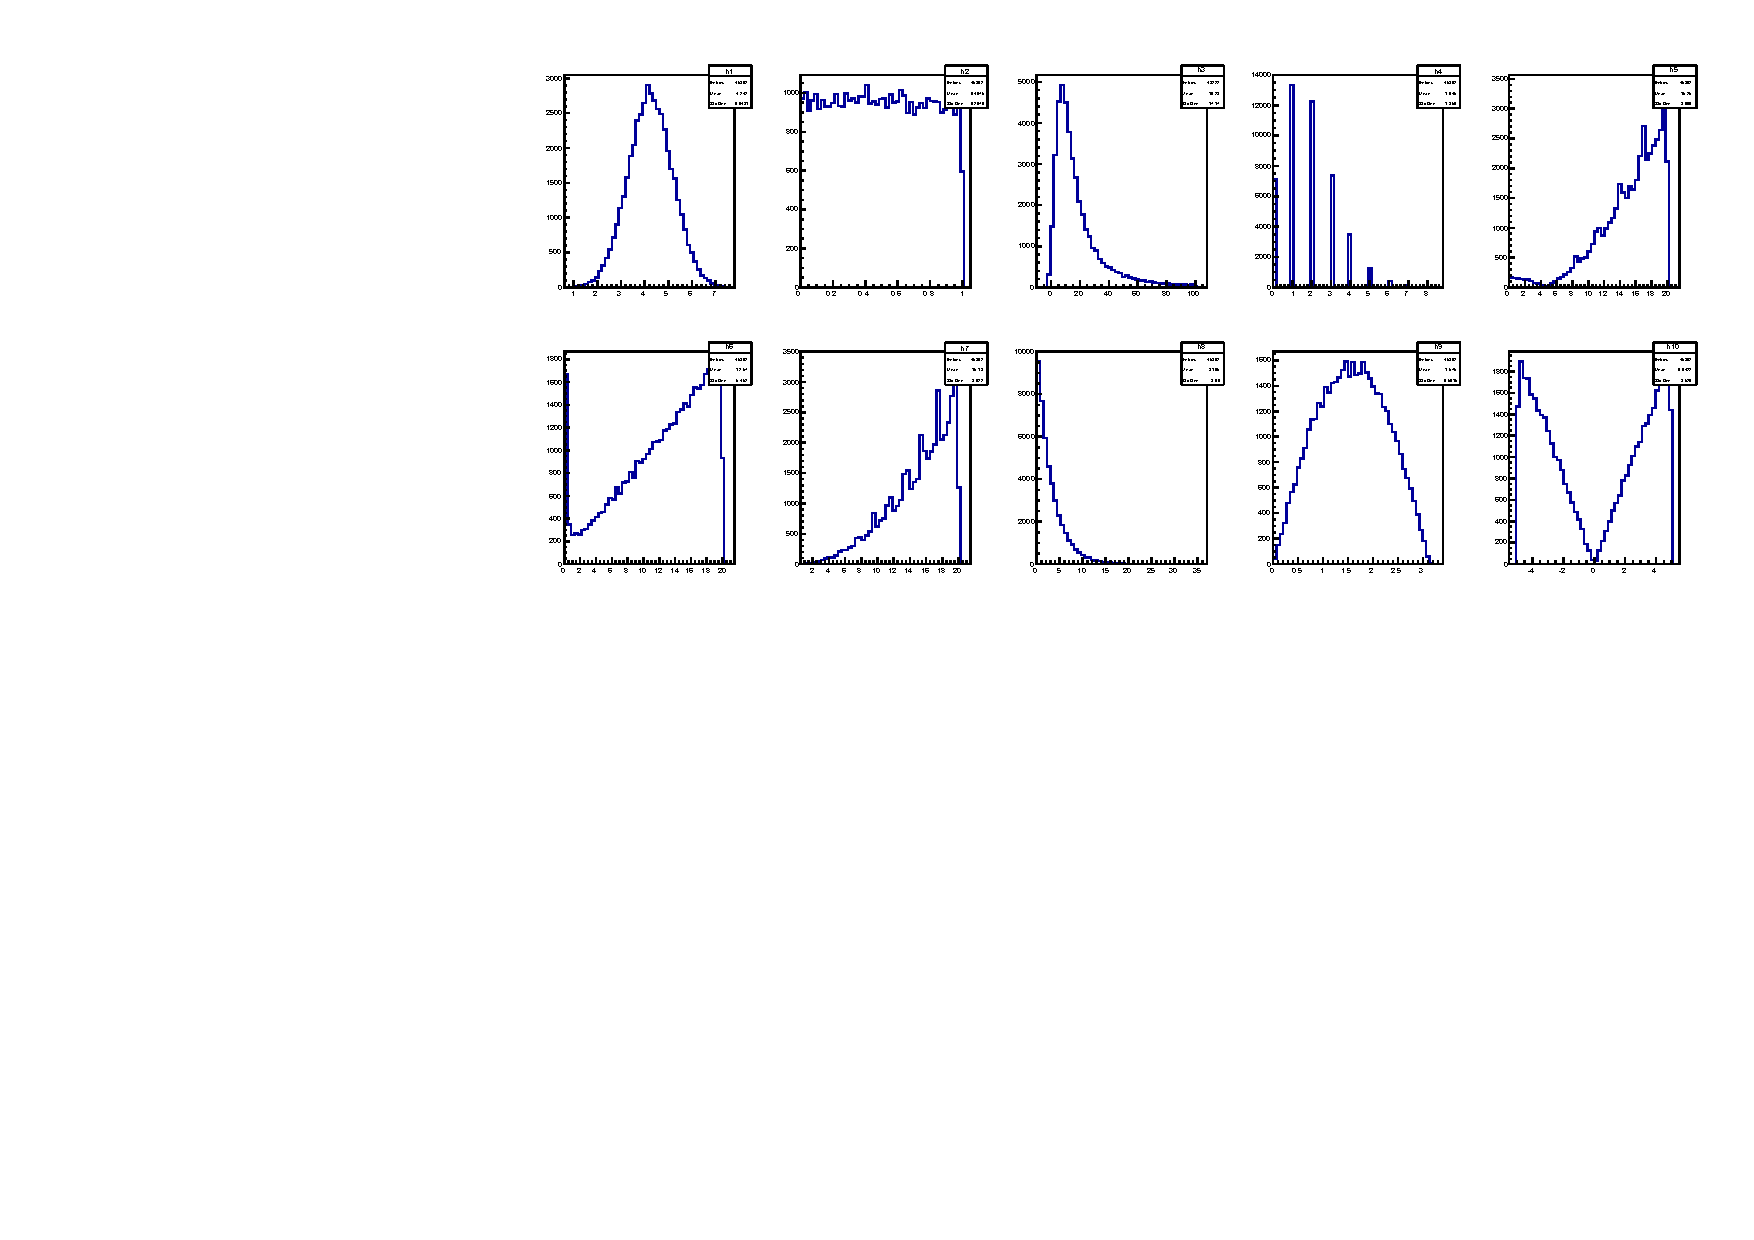
\includegraphics[scale=0.7]{Pictures/10histo.pdf}
\caption{Esempio di 10 istogrammi nella stessa canvas. \label{10h}}
\end{figure}
Il risultato delle 10 figure in un solo file è riportato in Figura \ref{10h}. La qualità della figura nel suo complesso è modesta, ma più avanti nel corso vedremo che i metodi offerti da root consentono di produrre figure di altissima qualità e leggibilità.

\section{Scrittura dati e istogrammi in un root-file}

Di seguito vedremo come root fornisca attraverso la classe TFile la possibilità di immagazzinare dati (anche le classi sono dati) in un file binario, leggero e di velocissimo accesso.

\begin{lstlisting}[language=c++]
{//inizio della macro
	//apriamo il file che conterra' i nostri dati
TFile * lino = new TFile("lino.root","recreate");
//Stuttura ad albero per accumulare i dati
TTree *hpp = new TTree("hpp","hpp");
//variabile di lettura dei dati, in questo caso uno solo 
//ma potrebbero esser molti di piu'
float evento;
//agganciamo la variabile ad un ramo della struttura hpp
hpp->Branch("evento",&evento,"evento/F");
ifstream leggo("dati1x.dat");

if(leggo.fail())
	{
	cout<<"non riesco a trovare il file o il file e' corrotto \n";
	}
//il ciclo procede a leggere l'evento
while (leggo>>evento)
	{
	hpp->Fill();//questo comando registra dentro il TTree i dati
	}
//Nota 
hpp->Write();//stampa i dati nel TFile attivo, in questo caso lino
lino->Close();//chiudiamo il file
}//fine della macro
\end{lstlisting}

La generalizzazione a più variabili è semplice:

\begin{lstlisting}[language=c++]
{
TTree *hpp = new TTree("hpp","hpp");
float evento1,evento2,evento3,evento4,evento5,evento6,evento7,evento8,evento9,ev
ento10;
hpp->Branch("evento1",&evento1,"evento1/F");
hpp->Branch("evento2",&evento2,"evento2/F");
hpp->Branch("evento3",&evento3,"evento3/F");
hpp->Branch("evento4",&evento4,"evento4/F");
hpp->Branch("evento5",&evento5,"evento5/F");
hpp->Branch("evento6",&evento6,"evento6/F");
hpp->Branch("evento7",&evento7,"evento7/F");
hpp->Branch("evento8",&evento8,"evento8/F");
hpp->Branch("evento9",&evento9,"evento9/F");
hpp->Branch("evento10",&evento10,"evento10/F");

ifstream leggo("datoni.dat");

if(leggo.fail())
	{
	cout<<"non riesco a trovare il file o il file e' corrotto \n";
	}

while (leggo>>evento1>>evento2>>evento3>>evento4>>evento5>>evento6>>evento7>>eve
nto8>>evento9>>evento10)
	{
	hpp->Fill();
	}

TFile * lino = new TFile("lino.root","recreate");
hpp->Write();
lino->Close();
}
\end{lstlisting}

Aprendo il file che contiene i dati può essere aperto da root, direttamente o attraverso una macro, utilizzando la classe TFile.
Direttamente scrivendo a terminale root nomedelfile.root (invio),
e in questo caso root ci fa la carezza di scrivere a posto nostro:\\
TFile \_file0 = new TFile::Open("nomedelfile.root");\\
oppure una volta che la sessione root è in corso aprendo il root file direttamente, anche senza passare dalla variabile puntatore, scrivendo:\\
TFile apriti("nomedelfile.root");\\
quest'ultimo comando funziona ovviamente anche all'interno di una macro di root.

Attraverso la classe TBrowser, che apre una interfaccia grafica, è possibile navigare all'interno del contenitore dei dati,
e nel caso in cui clicchiamo su una delle foglie (leaf) che rappresentano i dati, root automaticamente computa il corrispondente istogramma (vedi Figura \ref{screen2n}).

\begin{figure}
\centering
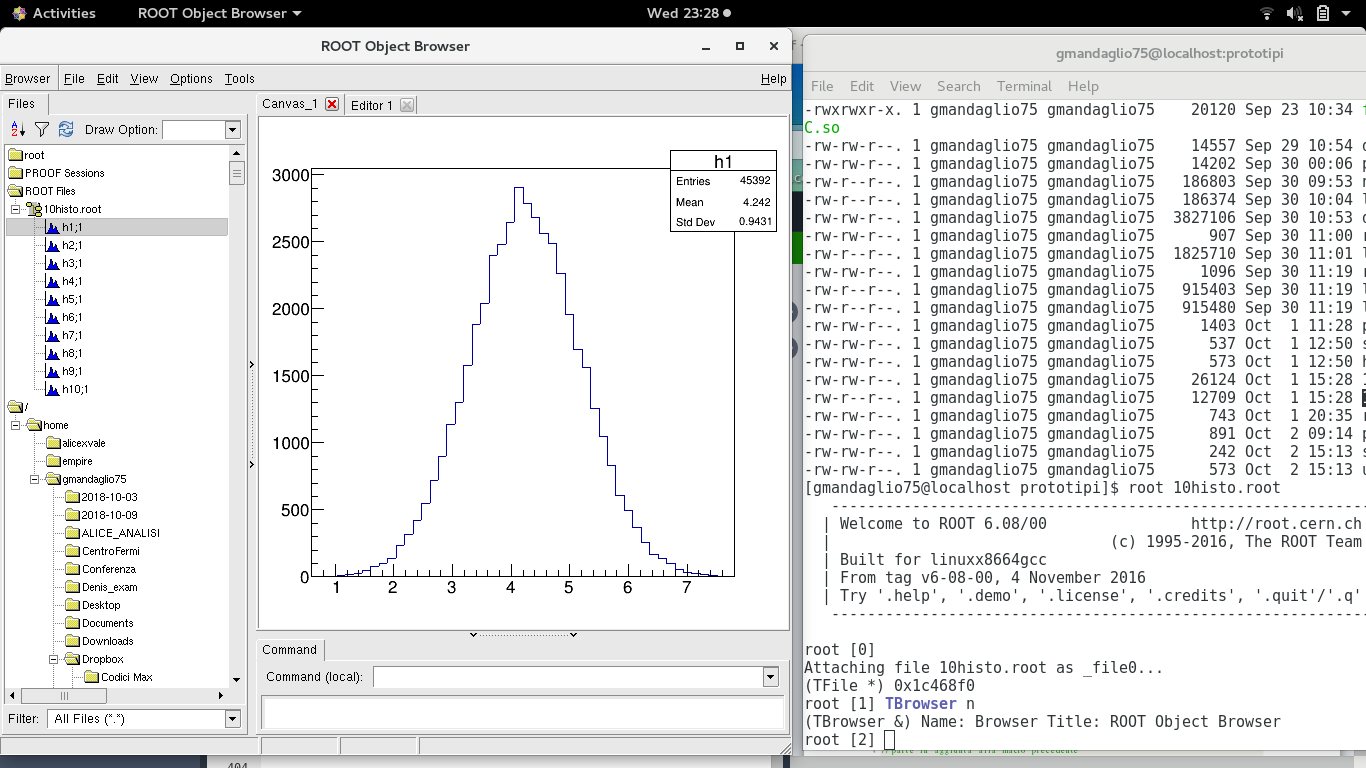
\includegraphics[scale=0.25]{Pictures/screen2n.png}
\caption{Lo screenshot mostra come aprire un root-file, e come navigarci dentro utilizzando la classe TBrowser. \label{screen2n}}
\end{figure}

Nel caso in cui volessimo immagazzinare istogrammi all'interno di un root-file, immaginando di aver usato un vettore di istogrammi, sarà sufficiente alla fine del codice aggiungere le seguenti righe di codice:
\begin{lstlisting}[language=c++]
{
....
TFile * pino = new TFile("10histo.root","recreate");
for(int i=0; i<10;i++){
 hist[i]->Write();
}
pino->Close();
\end{lstlisting}

Se provate a navigare nel root-file che contiene gli istogrammi, e cliccate da interfaccia grafica sul simbolo del dato istogramma,
vi apparirà l'istogramma, ma badate bene a non essere tratti in inganno con il caso precedente! Infatti, nel caso precedente anche quando cliccavamo sulla simbolo foglia ci appariva un istogramma, ma in questo caso la computazione dell'istogramma è online e la foglia rappresenta tutti i dati, nel caso dell'istogramma abbiamo solo le informazioni dell'istogramma ovvero i centri dei bin, le loro ampiezze e così via, ma abbiamo perso il dettaglio della distribuzione dei dati all'interno dei bin degli istogrammi.


\section{Scrittura e lettura su file dei dati di un istogramma}

La macro che viene descritta, apre un file root in cui abbiamo immagazzinato degli istogrammi, copia in una variabile indirizzo di tipo istogramma TH1D appena definito (per fare contento C++) l'indirizzo di un istogramma immagazzinato nel root file, dopo di che in un file di testo scrive il valore centrale di ogni bin e la frequenza assoluta di ogni bin. 

\begin{lstlisting}[language=c++]
{
TFile *ciao = new TFile("10histo.root");
ofstream scrivo("usciat.dat");
TH1D *copia = (TH1D*)ciao->Get("h1");
int stop =copia->GetNbinsX();
for(int i=1; i<stop; i++)
scrivo<<copia->GetBinCenter(i)<<"   "<<copia->GetBinContent(i)<<endl;
}
\end{lstlisting}

Il file di testo che abbiamo creato contiene tutte le informazioni necessarie dell'istogramma, nel senso che se noi inviassimo a un nostro collega questo file, lui sarebbe in grado di metterlo a grafico e analizzarlo. Volendo avremmo potuto scrivere solo la colonna delle frequenze assolute, ma in questo caso nella nostra ipotetica email al collega avremmo dovuto aggiungere come avevamo definito l'istogramma ovvero gli estremi dell'istogramma (il numero di bin in realtà è incluso nel numero di righe che abbiamo scritto nel file).


Volendo fare ora l'operazione inversa, e immaginando di avere solamente le due colonne di dati, proviamo a passare le informazioni alla classe che gestisce l'istogramma. Utilizziamo la classe vector per caricare i dati giusto per imparare a usare questa potentissima classe fornita dal c++, ovviamente avremmo potuto fare la stessa cosa per altre vie:

\begin{lstlisting}[language=c++]
{
ifstream leggo("usciat.dat");
vector<double> x,y;
double a,b;
while(leggo>>a>>b){
x.push_back(a); //inserisce dinamicamente una quantita'
y.push_back(b);
}
TH1D *h1 = new TH1D("h1","",x.size(),x.at(0)-(x.at(1)-x.at(0))/2.,x.at(a.size()-1)+(x.at(1)-x.at(0))/2.);
for(int i=1; i<x.size(); i++) //.size() mi dice quanti elementi abbiamo caricato
h1->SetBinContent(y.at(i));//notare la x l'abbiamo sistemata in fase di definizione
}
\end{lstlisting}

\section{L'algebra degli istogrammi}

Le classi TH1D tra i tanti metodi che forniscono, quali ad esempio ci dicono qual'è la media, la deviazione standard, il bin corrispondente al massimo etc., forniscono metodi che consentono anche di fare operazioni su istogrammi.
Negli esempi che illustreremo di seguito vedremo le operazioni di somma (Add), moltiplicazione per una costante (Scale), divisione (Divide),
moltiplicazione (Multiply). Di fatto qualunque operazione lineare ci viene in mente di fare su istogrammi lo possiamo fare.
L'unica regola che bisogna rispettare per utilizzare questi metodi è che gli istogrammi siano definiti nel medesimo intervallo di variabilità e che abbiano lo stesso numero di bin, non dimentichiamo che le operazioni avvengono bin per bin.

Prima di utilizzarli, prendiamola da lontano, e proviamo a fare il seguente esercizio: \textit{in due file daterelli.dat e daterelli2.dat, ci sono immagazzinati due set di dati, nel primo ci sono 4 colonne, nel secondo 2 colonne. Caricare i 6 gruppi di dati contenuti nei due file in 6 istogrammi definiti nell'intervallo da 0 a 10 e con 50 bin.}

Prima mostriamo la risoluzione lunga, con gli istogrammi singoli:


\begin{lstlisting}[language=c++]
{
//usiamo due variabili ifstream per leggere i dati
 ifstream leggo1("daterelli.dat");
 ifstream leggo2("daterelli2.dat");
 //prenotiamo 6 istogrammi come richiesto
TH1D *h1 = new TH1D("h1","",50,0,10);
TH1D *h2 = new TH1D("h2","",50,0,10);
TH1D *h3 = new TH1D("h3","",50,0,10);
TH1D *h4 = new TH1D("h4","",50,0,10);
TH1D *h5 = new TH1D("h5","",50,0,10);
TH1D *h6 = new TH1D("h6","",50,0,10);
//definiamo il massimo numero di variabili che ci servono per la lettura
double a,b,c,d;
//eseguiamo due cicli per la lettura dei dati e la computazione degli istogrammi
while(leggo2>>a>>b)
   {
   h1->Fill(a);
   h2->Fill(b);
   }
while(leggo1>>a>>b>>c>>d)
   {
   h3->Fill(a);
   h4->Fill(b);
   h5->Fill(c);
   h6->Fill(d);
   }
   //chiudiamo i file dopo l'utilizzo
   leggo1.close();
   leggo2.close();
   
   //questo per averli tutti nella stessa scatola (canvas)
TCanvas *tutti = new TCanvas("tutti","",1200,1000);
//dividiamo la scatola
tutti->Divide(2,3);
//con cd ci muoviamo nelle sotto settori della scatola
tutti->cd(1);
h1->Draw();
tutti->cd(2);
h2->Draw();
tutti->cd(3);
h3->Draw();
tutti->cd(4);
h4->Draw();
tutti->cd(5);
h5->Draw();
tutti->cd(6);
h6->Draw();
}
\end{lstlisting}

questa è la stessa versione del programma affrontato utilizzando i vettori di istogrammi, come potrete notare il codice risulta molto più piccolo, e come vedrete più facilmente modificabile:

\begin{lstlisting}[language=c++]
{
{
//usiamo due variabili ifstream per leggere i dati
 ifstream leggo1("daterelli.dat");
 ifstream leggo2("daterelli2.dat");
 //dichiariamo un vettore di 6 indirizzi a variabile di tipo TH1D
TH1D *histo[6];
//riempiamo con un ciclo le variabili appena dichiarate
//Utilizziamo Form per creare dinamicamente le label interne degli istogrammi
//se definiamo due istogrammi con la stessa label interna, root da errore!!!
for(int i =0; i<6;i++){
histo[i] = new TH1D(Form("h%d",i+1),"",50,0,10);
}
//definiamo il massimo numero di variabili che ci servono per la lettura
double a,b,c,d;
//eseguiamo due cicli per la lettura dei dati e la computazione degli istogrammi
while(leggo1>>a>>b>>c>>d)
   {
   histo[2]->Fill(a);
   histo[3]->Fill(b);
   histo[4]->Fill(c);
   histo[5]->Fill(d);
   }
while(leggo2>>a>>b)
   {
   histo[0]->Fill(a);
   histo[1]->Fill(b);
   }
//chiudiamo i file dopo l'utilizzo
leggo1.close();
leggo2.close();
   //questo per averli tutti nella stessa scatola (canvas)
TCanvas *tutti = new TCanvas("tutti","",1200,1000);
//dividiamo la scatola
tutti->Divide(2,3);
//eseguiamo un ciclo per caricare le figure nei settori della scatola
for(int i =0; i<6;i++){
//con cd ci muoviamo nelle sotto settori della scatola
tutti->cd(i+1);
histo[i]->Draw();
}
//salviamo la nostra figura in un file in formato pdf (sono disponibili svariati formati: jpg, png, esp, ps etc)
tutti->SaveAs("figuratutti.pdf");
//da questo punto a seguire della macro, gli istogrammi sono stati computati e quindi sono disponibili per le nostre analisi
}
\end{lstlisting}

Nella figura \ref{fig6h1} sono rappresentati gli istogrammi che abbiamo appena computato. I primi due istogrammi in alto sono ottenuti dal file daterelli2.dat (2 colonne), i rimanenti dal file daterelli.dat (4 colonne). Osservando queste figure vi invito a trovare le familiarità che hanno.
\begin{figure}[h]
\centering
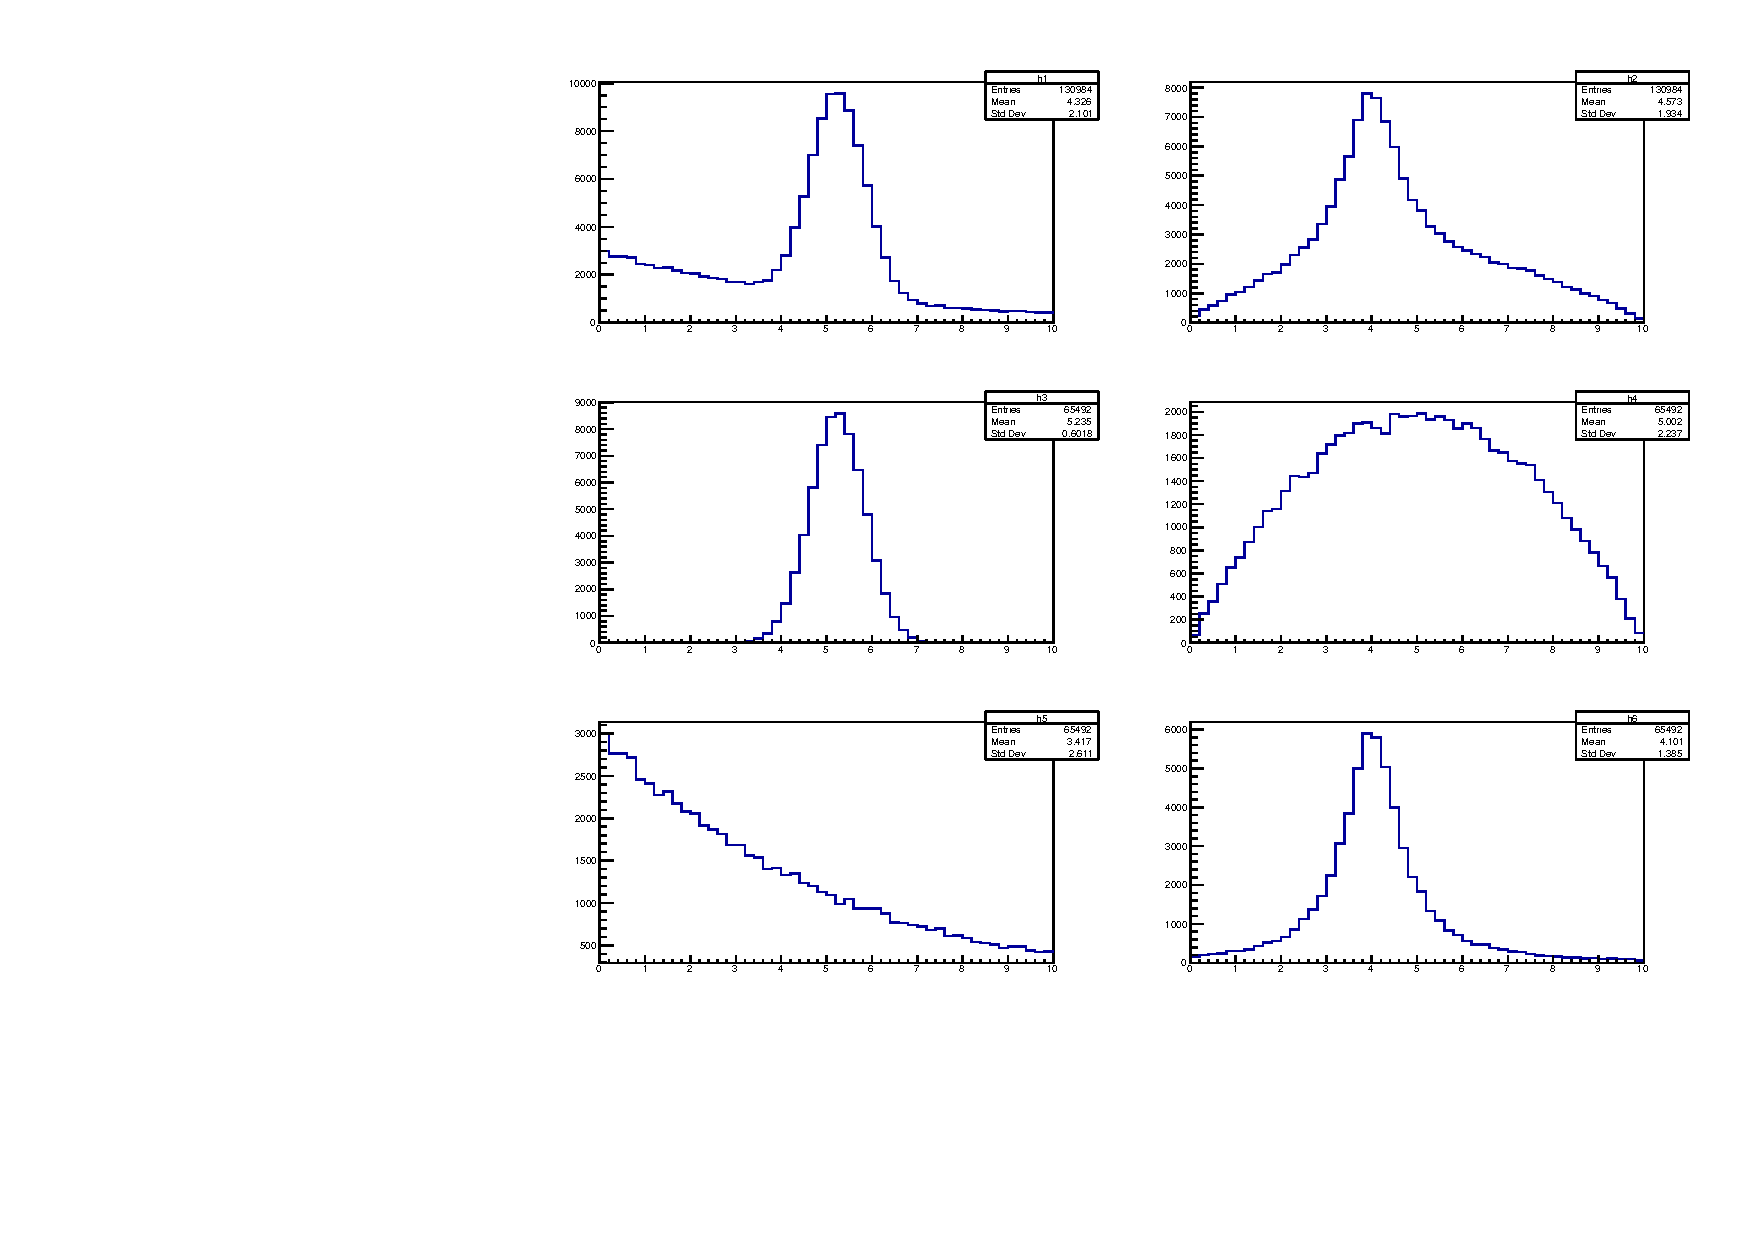
\includegraphics[scale=0.8]{Pictures/figuratutti.pdf}
\caption{Rappresentazione nella stessa canvas dei 6 istogrammi caricati dai due file daterelli.dat e daterelli2.dat. \label{fig6h1}}
\end{figure}

Non vi viene in mente nulla? .... Nessun problema proviamo a mettere a grafico i nostri risultati in modo più leggibile, ad esempio, forzando le scale dei conteggi ad essere tutti uguali e pari a quelle dell'istogramma che presenta il massimo valore, che nel nostro caso è l'istogramma 1 (in questo caso 10000).

Per effettuare la forzatura sull'asse dei conteggi abbiamo aggiunto semplicemente la riga che vedete:
\begin{lstlisting}[language=c++]
{
.....
......
for(int i =0; i<6;i++){
tutti->cd(i+1);
//aggiungiamo nel ciclo questa istruzione che consente di forzare l'asse y nel medesimo range di variabilita'
histo[i]->GetYaxis()->SetRangeUser(0,10000);
histo[i]->Draw();
}
tutti->SaveAs("figuratutti2.pdf");
}
\end{lstlisting}

Il risultato è presentato in figura \ref{fig6h2}. In questa nuova figura le informazioni riportate sono le stesse di quella precedente, ma come possiamo notare risulta essere di più facile lettura. Infatti, dopo averla osservata per qualche istante, subito ci accorgiamo che l'istogramma 1 sembra essere dato dalla somma dell'istogramma 3 e dall'istogramma 5, mentre l'istogramma 2 come la somma del 4 e del 6.
L'impressione è esatta perchè i file dei dati sono stati creati immagazzinando nel file a 4 colonne i quattro istogrammi componenti, mentre nel file a due colonne sono state copiate i dati degli istogrammi 3 e 5 nella prima colonna mentre quelli del 4 e 6 nella seconda colonna.  
\begin{figure}[h]
\centering
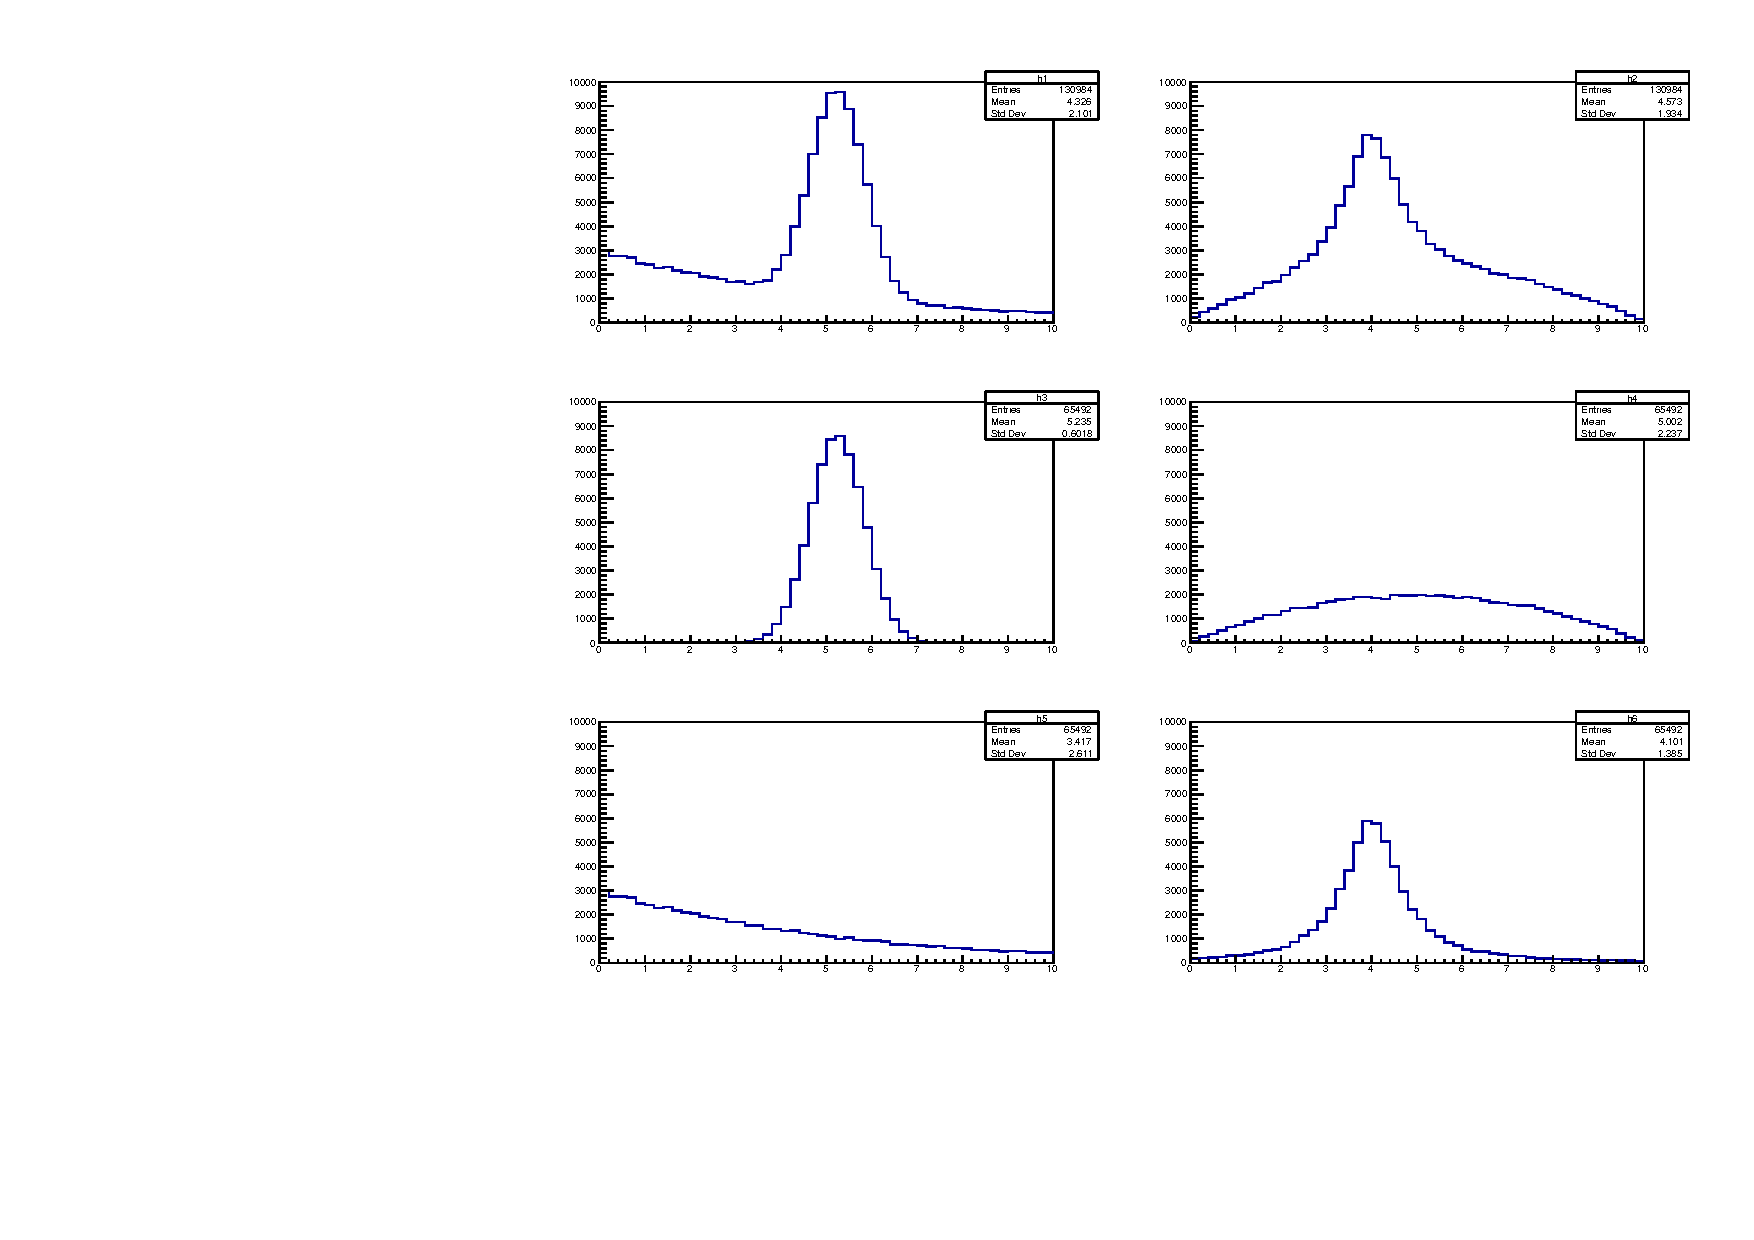
\includegraphics[scale=0.8]{Pictures/figuratutti2.pdf}
\caption{Rappresentazione nella stessa canvas dei 6 istogrammi caricati dai due file daterelli.dat e daterelli2.dat, con lo stesso intervallo di variabilità per l'asse y. \label{fig6h2}}
\end{figure}
Questi oggetti che abbiamo computato rappresentano un'occasione ideale per mettere alla prova il metodo di somma offerto dalla classe TH1D.

la somma di istogrammi si effettua attraverso il metodo somma \textbf{Add} di seguito riportiamo due delle sue definizioni:
\begin{lstlisting}[language=c++]
//Queste due delle definizioni del metodo
//le costanti se non definite nel momento dell'uso per default sono prese pari a 1
Bool_t Add(const TH1* h, const TH1* h2, Double_t c1 = 1, Double_t c2 = 1) 	// *MENU*
Bool_t Add(const TH1* h1, Double_t c1 = 1)
\end{lstlisting}
la prima definizione vediamo che il metodo restituisce un valore logico che ci dice se l'operazione è andata a buon fine o no, mentre come informazioni di input desidera due puntatori a istogrammi, e due costanti moltiplicative dei rispettivi istogrammi, questa definizione del metodo in pratica realizza quella che chiamiamo combinazione lineare $h3 = c1 \cdot h1 + c2 \cdot h2$, comprendiamo subito che grazie a questa definizione del metodo possiamo effettuare le operazioni di somma e sottrazione pesate.

Il secondo metodo invece consente di sommare all'istogramma che invoca questo metodo con questa sintassi, l'istogramma che diamo come input al metodo: $h2 = h2 + c1 \cdot h1$.

Ora come esercizio proviamo a mettere nello stesso grafico l'istogramma h1 e a sovrapporgli la differenza tra l'istogramma h1 e h3, e vediamo cosa succede:


\begin{lstlisting}[language=c++]
//immaginiamo di essere in coda ai codici che hanno computato gli istogrammi
//Definiamo un istogramma nello stesso modo con cui sono stati definiti
//gli istogrammi che saranno oggetto della somma
TH1D *somma = new TH1D("somma","",50,0,10);
//Usiamo il metodo Add, ma notiamo che il coefficiente c2 in questo caso e' -1
somma->Add(h1,h3,1,-1);//c2=-1 definisce una sottrazione
//usiamo i metodi SetLine... per rendere le figure piu' visibili
h1->SetLineColor(1);
h1->SetLineStyle(1);
h1->SetLineWidth(2);
somma->SetLineColor(2);
somma->SetLineStyle(2);
somma->SetLineWidth(2);
//creiamo una scatola
TCanvas *sss = new TCanvas("sss","",1200,1000);
//stampiamo il grafico sorgente
h1->Draw();
//Stampiamo il grafico risultato della nostra sottrazione
somma->Draw("same");//l'opzione same sovrappone evita che sostituisca
//Salviamo il file che inseriremo in questo manuale
sss->SaveAs("diffhisto1.pdf");
\end{lstlisting}


\begin{figure}[h]
\centering
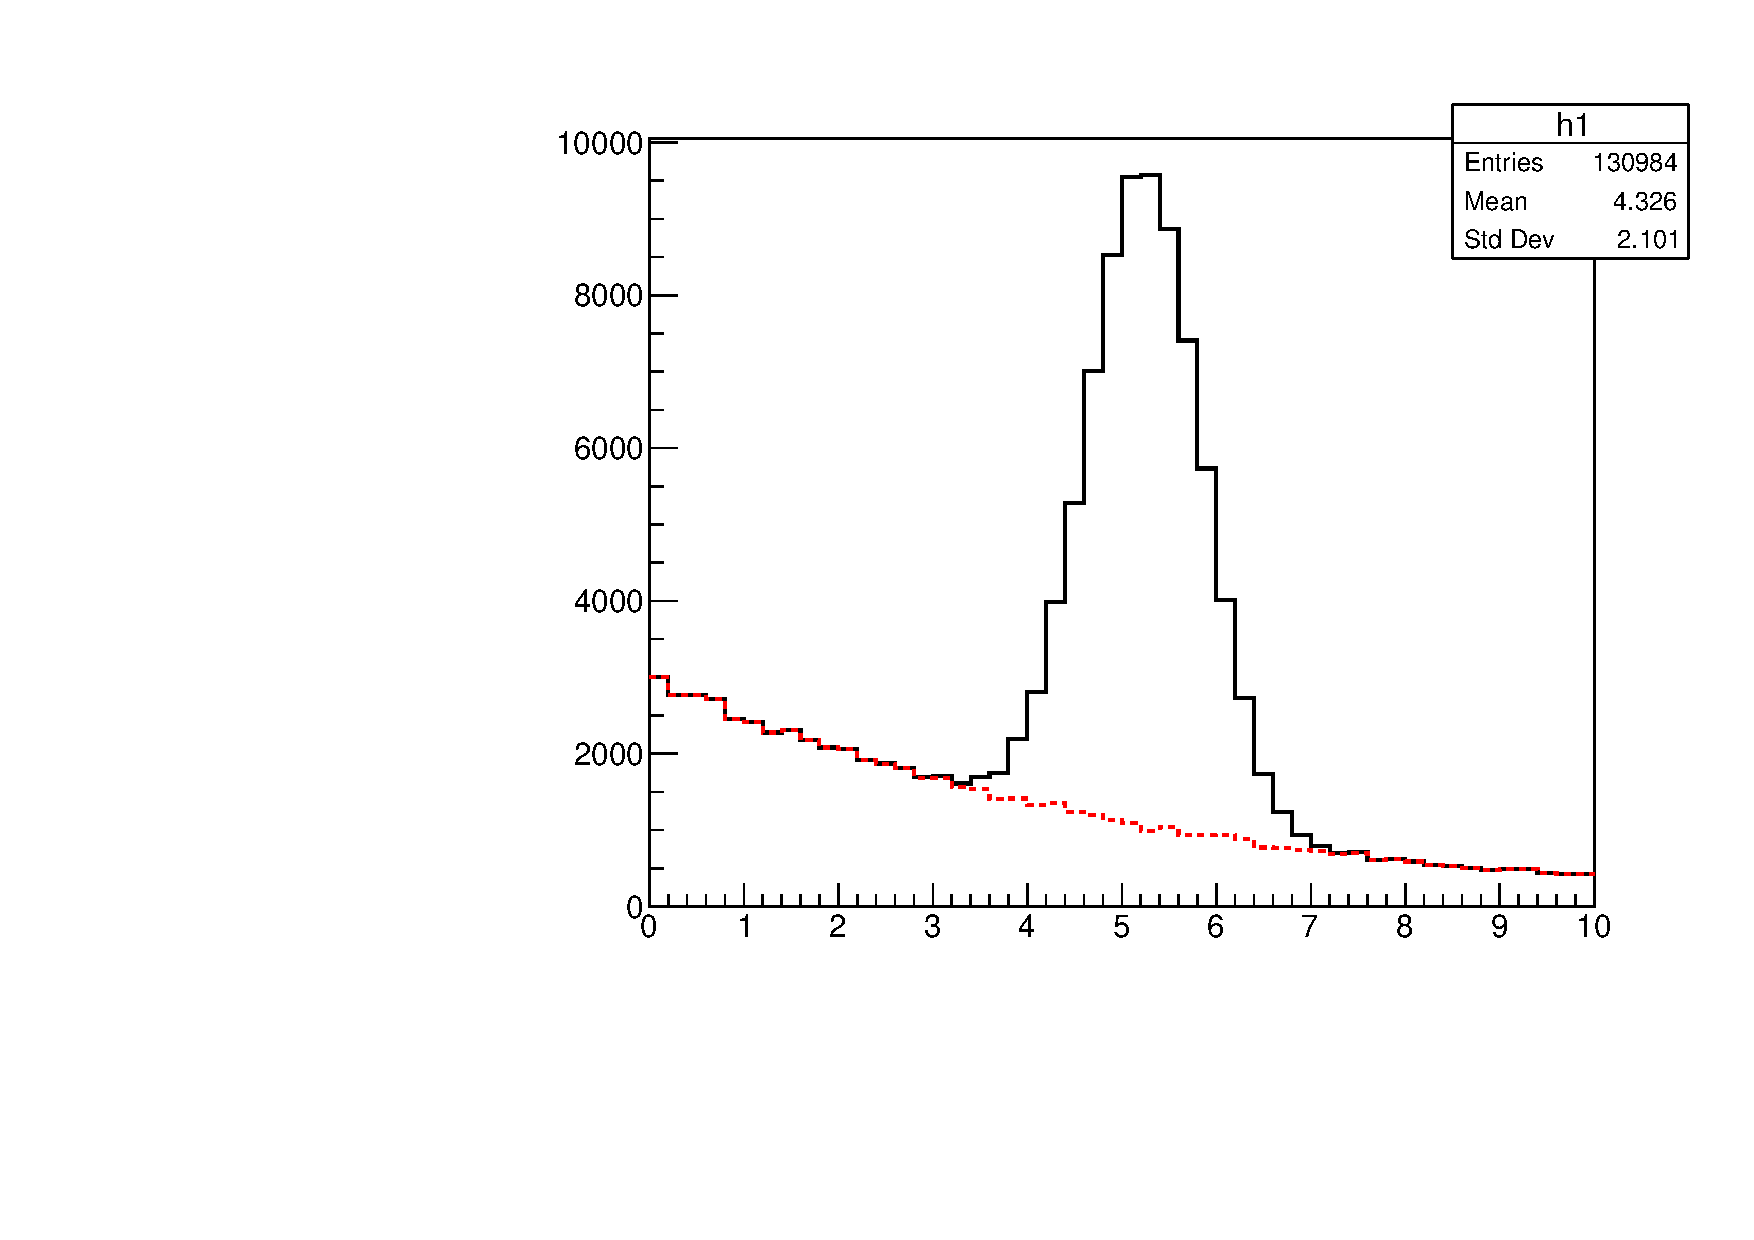
\includegraphics[scale=0.5]{Pictures/diffhisto1.pdf}
\caption{La linea continua rappresenta l'istogramma h1, mentre la linea tratteggiata è il risultato di h1-h3 \label{diff}}
\end{figure}

Come possiamo osservare in Figura \ref{diff} la curva tratteggiata, ottenuta come sottrazione dell'istogramma h3 ad h1, risulta essere coincidente con l'istogramma h5. Se si è increduli, cosa buona e giusta, allora per esercizio si potrebbe provare a mettere nelle stesso grafico l'istogramma che abbiamo chiamato somma (h1-h3) con l'istogramma h5 e verificare se coincidono (nota: quando lo fate cambiate lo stile delle curve, altrimenti a causa del fatto che le curve sono esattamente coincidenti, nella sovrapposizione potreste essere autorizzati a pensare di aver perso una curva).
Un altro utile esercizio potrebbe essere ripetere quanto fatto con gli istogrammi 2, 4 e 6.

\begin{figure}[h]
\centering
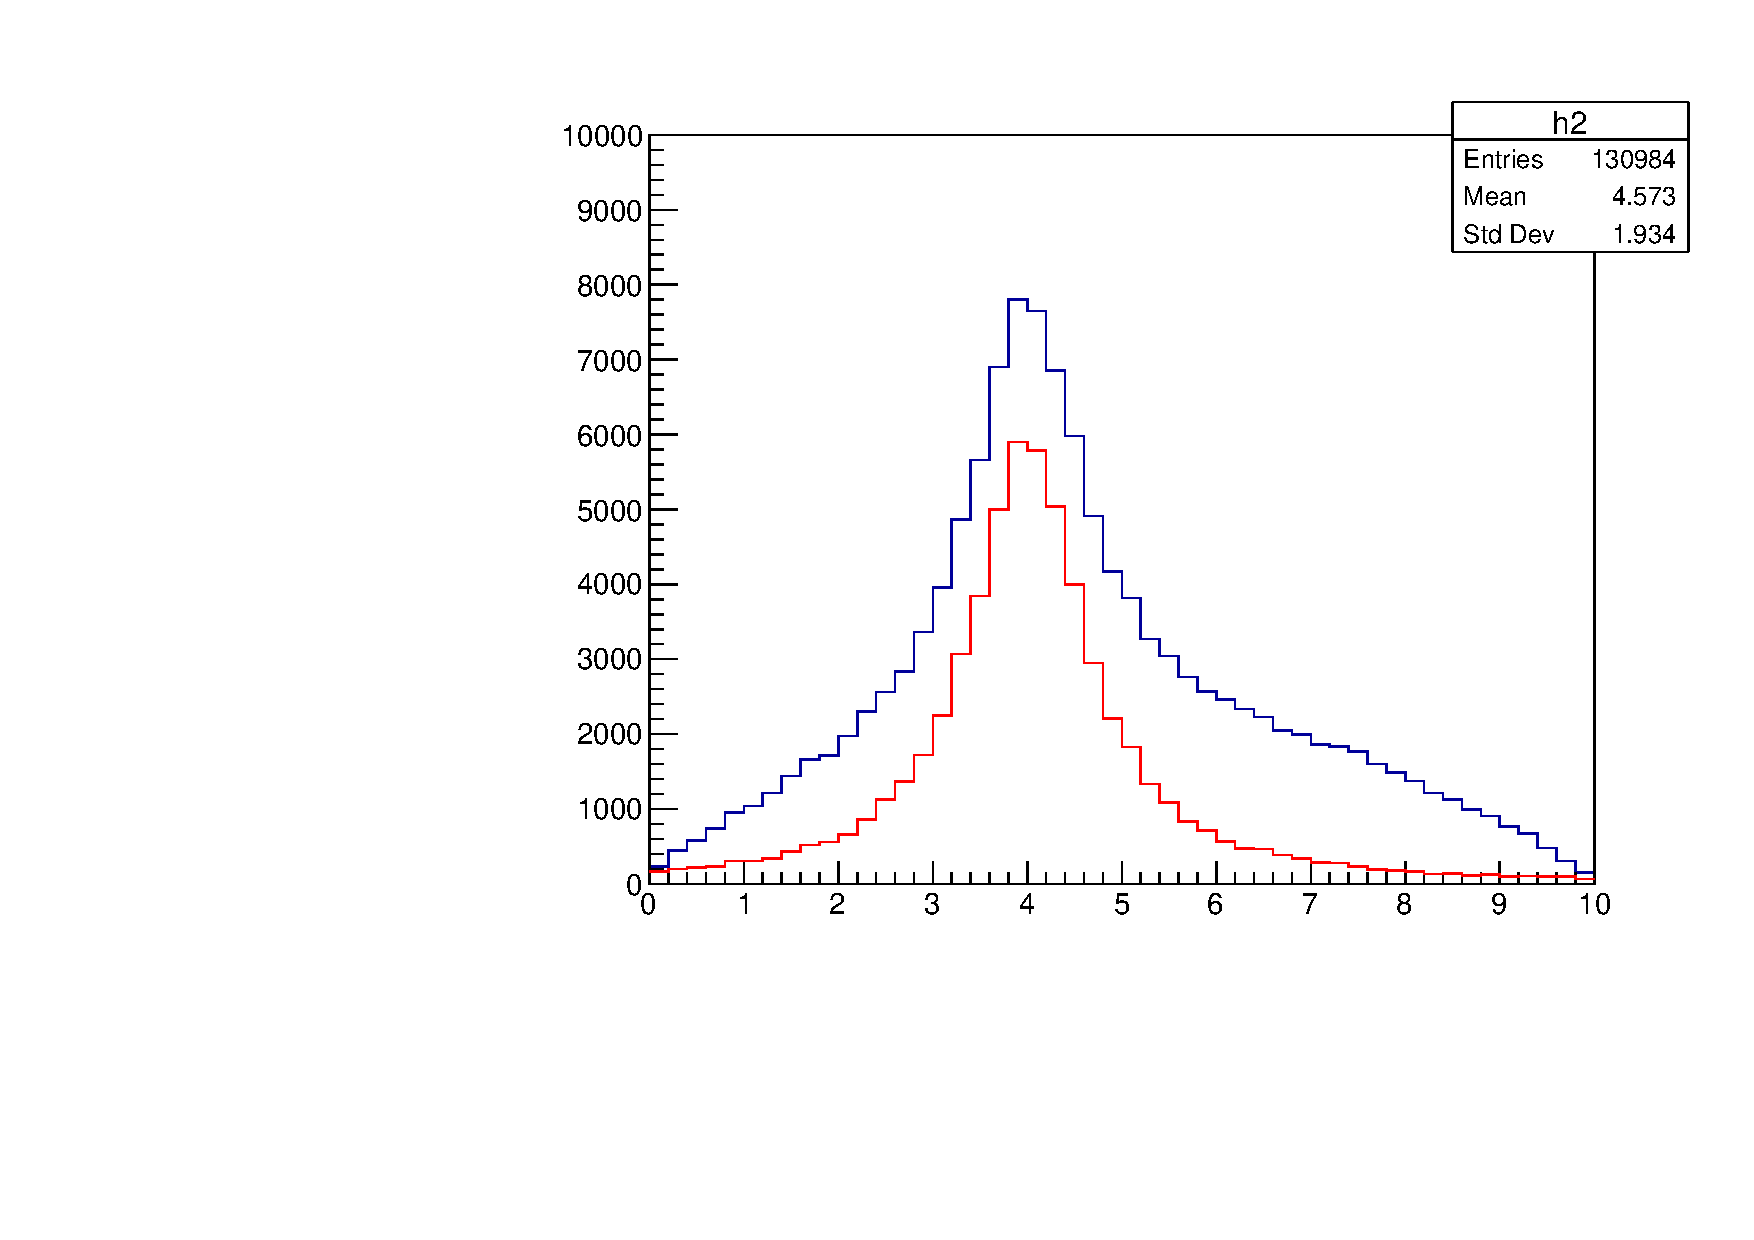
\includegraphics[scale=0.35]{Pictures/diff3.pdf}
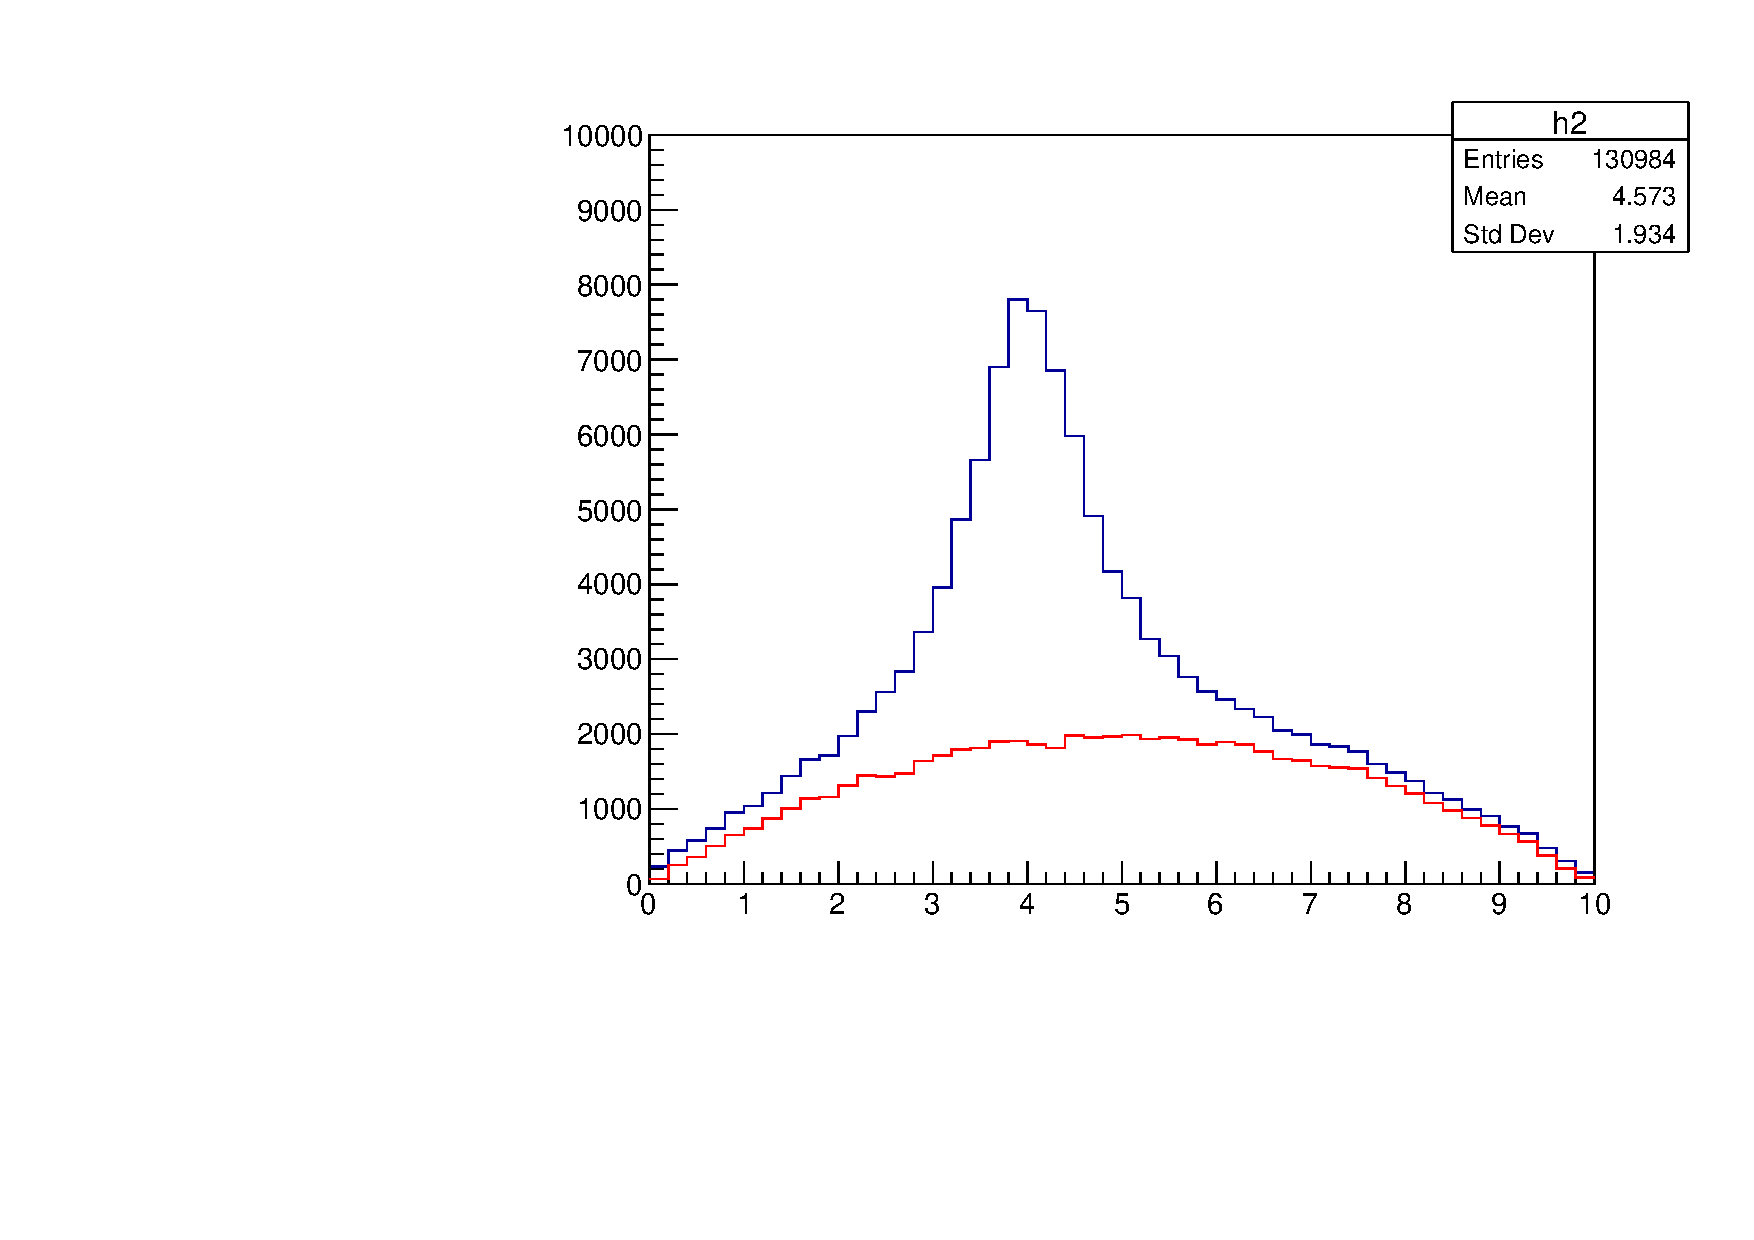
\includegraphics[scale=0.35]{Pictures/diff4.pdf}
\caption{La linea blu rappresenta l'istogramma h2, mentre la linea rossa è il risultato di h2-h4 a sinistra e h2-h6 a destra.   \label{diff2}}
\end{figure}

\section{Classe TF1, funzioni e funzioni parametriche}

La classe TF1 consente di costruire oggetti che detengono una funzione definita in un dato intervallo di variabilità secondo le esigenze dell'utente che le implementa. La sintassi di uno dei costruttori, il più semplice, quello che utilizzeremo in questo paragrafo è la seguente:

\begin{lstlisting}[language=c++]
//costruttore
TF1(const char* name, const char* formula, Double_t xmin = 0, Double_t xmax = 1, TF1::EAddToList addToGlobList = EAddToList::kDefault)
//esempio di funzione non parametrica, l'ultima opzione l'abbiamo omessa e lui assume quella di default.
TF1 *funzione1 = new TF1("funzione1","sin(x)/x",-10,10);
//esempio di funzione parametrica 
TF1 *funzione2 = new TF1("funzione2","[0]*exp(-pow(x-[1],2)/[2]",0,7.4);
//in questo caso abbiamo 3 parametri: [0], [1], [2]
\end{lstlisting}

Le funzioni implementate attraverso la classe TF1 possono essere rappresentate, utilizzate per generare una successione di valori, e possono essere utilizzati, nel caso delle funzioni parametriche, come modelli per rappresentare dei dati, vedremo in seguito che possono anche essere utilizzate  per generare distribuzioni di dati che obbediscono alla funzione densità di probabilità che rappresentano. 



\section{Modellizzazione di dati attraverso procedure di fit}

Come primo esercizio, utilizzeremo gli istogrammi riportati in figura \ref{fig6h1} per cercare di rispondere alla domanda: \textit{gli andamenti di questi istogrammi possono essere rappresentati da una funzione? I parametri di questa funzione, hanno un significato? Possono essere considerati essi stessi una misura?}.

Tra le forme riportate in figura \ref{fig6h1}, le più semplici potrebbero essere quelle degli istogrammi 3 e 4. Il primo sembra avere la forma di una Gaussiana, il secondo di una parabola, o se vogliamo di un polinomio di secondo grado.

Per le forme standard, ROOT fornisce attraverso delle parole chiave l'implementazione di funzioni come la Gaussiana, i polinomi fino al grado 9, e altre funzioni. Quindi per ricavare i parametri della funzione Gaussiana che potrebbe rappresentare la distribuzione del terzo istogramma, basta scrivere il codice:


\begin{lstlisting}[language=c++]
{
 ifstream leggimi("daterelli2.dat");
 //dichiariamo un vettore di 4 indirizzi a variabile di tipo TH1D
TH1D *histo[4];
//riempiamo con un ciclo le variabili appena dichiarate
for(int i =0; i<4;i++){
histo[i] = new TH1D(Form("h%d",i+1),"",50,0,10);
}
//definiamo il massimo numero di variabili che ci servono per la lettura
double a,b,c,d;
//eseguiamo due cicli per la lettura dei dati e la computazione degli istogrammi
while(leggimi>>a>>b>>c>>d)
   {
   histo[0]->Fill(a);
   histo[1]->Fill(b);
   histo[2]->Fill(c);
   histo[3]->Fill(d);
   }
//chiudiamo il file dopo l'utilizzo
leggimi.close();

TCanvas *box = new TCanvas("box","",600,500);

histo[2]->Draw();

//utilizziamo direttamente la parola chiave gaus per 
//produrre un fit con una Gaussiana senza passare per una TF1
histo[0]->Fit("gaus");
box->SaveAs("fitgaus.pdf");
}
\end{lstlisting}

Il risultato che otteniamo facendo girare a ROOT il piccolo codice che abbiamo appena scritto è riportato in figura \ref{fitbabbo1}.


\begin{figure}[h]
\centering
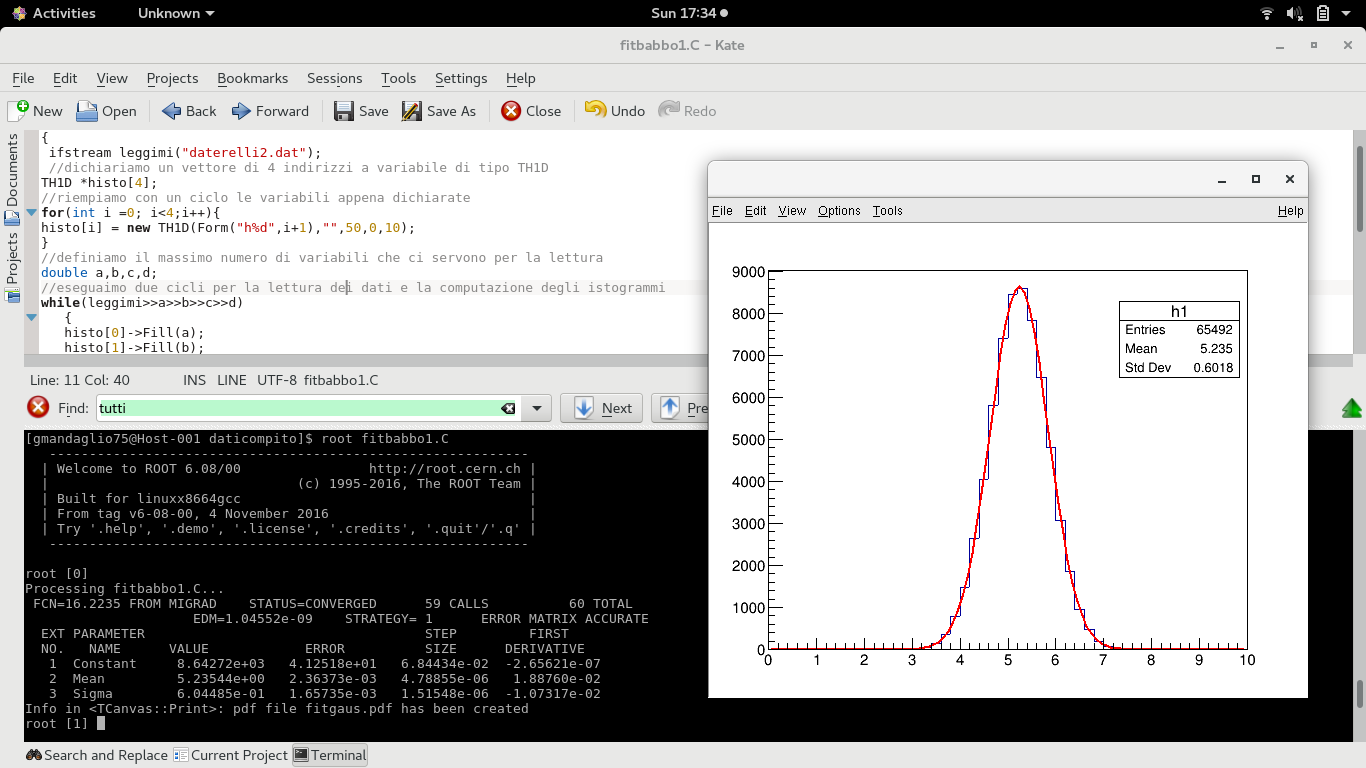
\includegraphics[scale=0.3]{Pictures/fitbabbo1.png}
\caption{Screenshot che mostra l'esecuzione del codice che produce il fit della Gaussiana.   \label{fitbabbo1}}
\end{figure}

Come si può notare nello screenshot in figura \ref{fitbabbo1}, il codice dopo aver computato l'istogramma e averlo visualizzato attraverso il metodo Draw(), attraverso il metodo Fit, con argomento la parola chiave \textit{gaus}, ha prodotto una curva rossa che si è sovrapposta al grafico dell'istogramma, con ottimo accordo in questo caso. L'interprede di root ha inoltre stampato nel terminale una serie di informazioni statistiche di grande utilità: FNC ci dice il $\chi^2$ del fit, ci dice quale algoritmo di minimizzazione ha utilizzato (MIGRAD), quante iterazione ha compiuto prima di convergere al risultato, e infine la lista dei parametri della funzione con relativi errori. 
Le quantità che l'interprete scrive a schermo possono essere utilizzate all'interno del nostro codice chiedendole alla funzione utilizzate per il fit, utilizzando i metodi \textit{GetParameter(numero intero partendo da zero che individua il parametro)}, \textit{GetParameters(indirizzo del vettore di reali, di dimensione pari al numero di parametri)}, \textit{GetChisquare()} che restituisce il $\chi^2$, \textit{GetNDF()} che restituisce i gradi di libertà del fit\footnote{Importante conoscere i gradi di libertà del fit. In particolare vi consente di calcolare il $chi^2$ ridotto, che è dato dal $\chi^2$ diviso il numero dei gradi di libertà.}

\begin{lstlisting}[language=c++]
{
......
......
Continuando dal codice precedente
......
......
TCanvas *box = new TCanvas("box","",600,500);

histo[2]->Draw();

//utilizziamo direttamente la parola chiave gaus per 
//produrre un fit con una Gaussiana senza passare per una TF1
histo[0]->Fit("gaus");
box->SaveAs("fitgaus.pdf");
cout<<"il chi2 del fit e' "<<gaus->GetChisquare()<<endl;
//il parametro 0 e' l'ampiezza della Gaussiana
cout<<"il valore medio della Gaussiana e' "<<gaus->GetParameter(1)<<endl;
cout<<"La deviazione standard della Gaussiana e' "<<gaus->GetParameter(2)<<endl;
}
\end{lstlisting}
Ovviamente avremmo potuto implementare la funzione Gaussiana in modo indipendente:
\begin{lstlisting}[language=c++]
{
double low=0., high=100.; //gli estremi dell'intervallo di definizione della funzione
TF1 *funz = new TF1("funz","[0]*exp(-pow(x-[1],2)/[2]),low,high);
}
\end{lstlisting}

Altrettanto semplice è il fit dell'istogramma hist[1], questo ha chiaramente l'andamento di una parabola e utilizzando la parola chiave pol2 come argomento del metodo Fit, questo immediatamente restituisce il fit corretto, lascio a voi questo semplice esercizio.
In questo semplice esempio non abbiamo incontrato particolari problemi, la distribuzione è stata prodotta con un toy-montecarlo che generava una Gaussiana, la stessa cosa la potrete osservare ripetendo l'esercizio per il secondo istogramma utilizzando una parabola. Quindi in questi due esempi non abbiamo avuto difficoltà a portare a casa i fit, ma vedremo in seguito che non è sempre così semplice.


Ora proviamo a modellizzare con un fit gli ultimi due istogrammi di figura \ref{fig6h1}, il quinto istogramma proviamo con un retta mentre per il sesto insistiamo con una Gaussiana vista la forma a picco dell'istogramma in esame,
il risultato del nostro tentativo lo riportiamo in figura \ref{fitbabbo2}.

\begin{figure}[h]
\centering
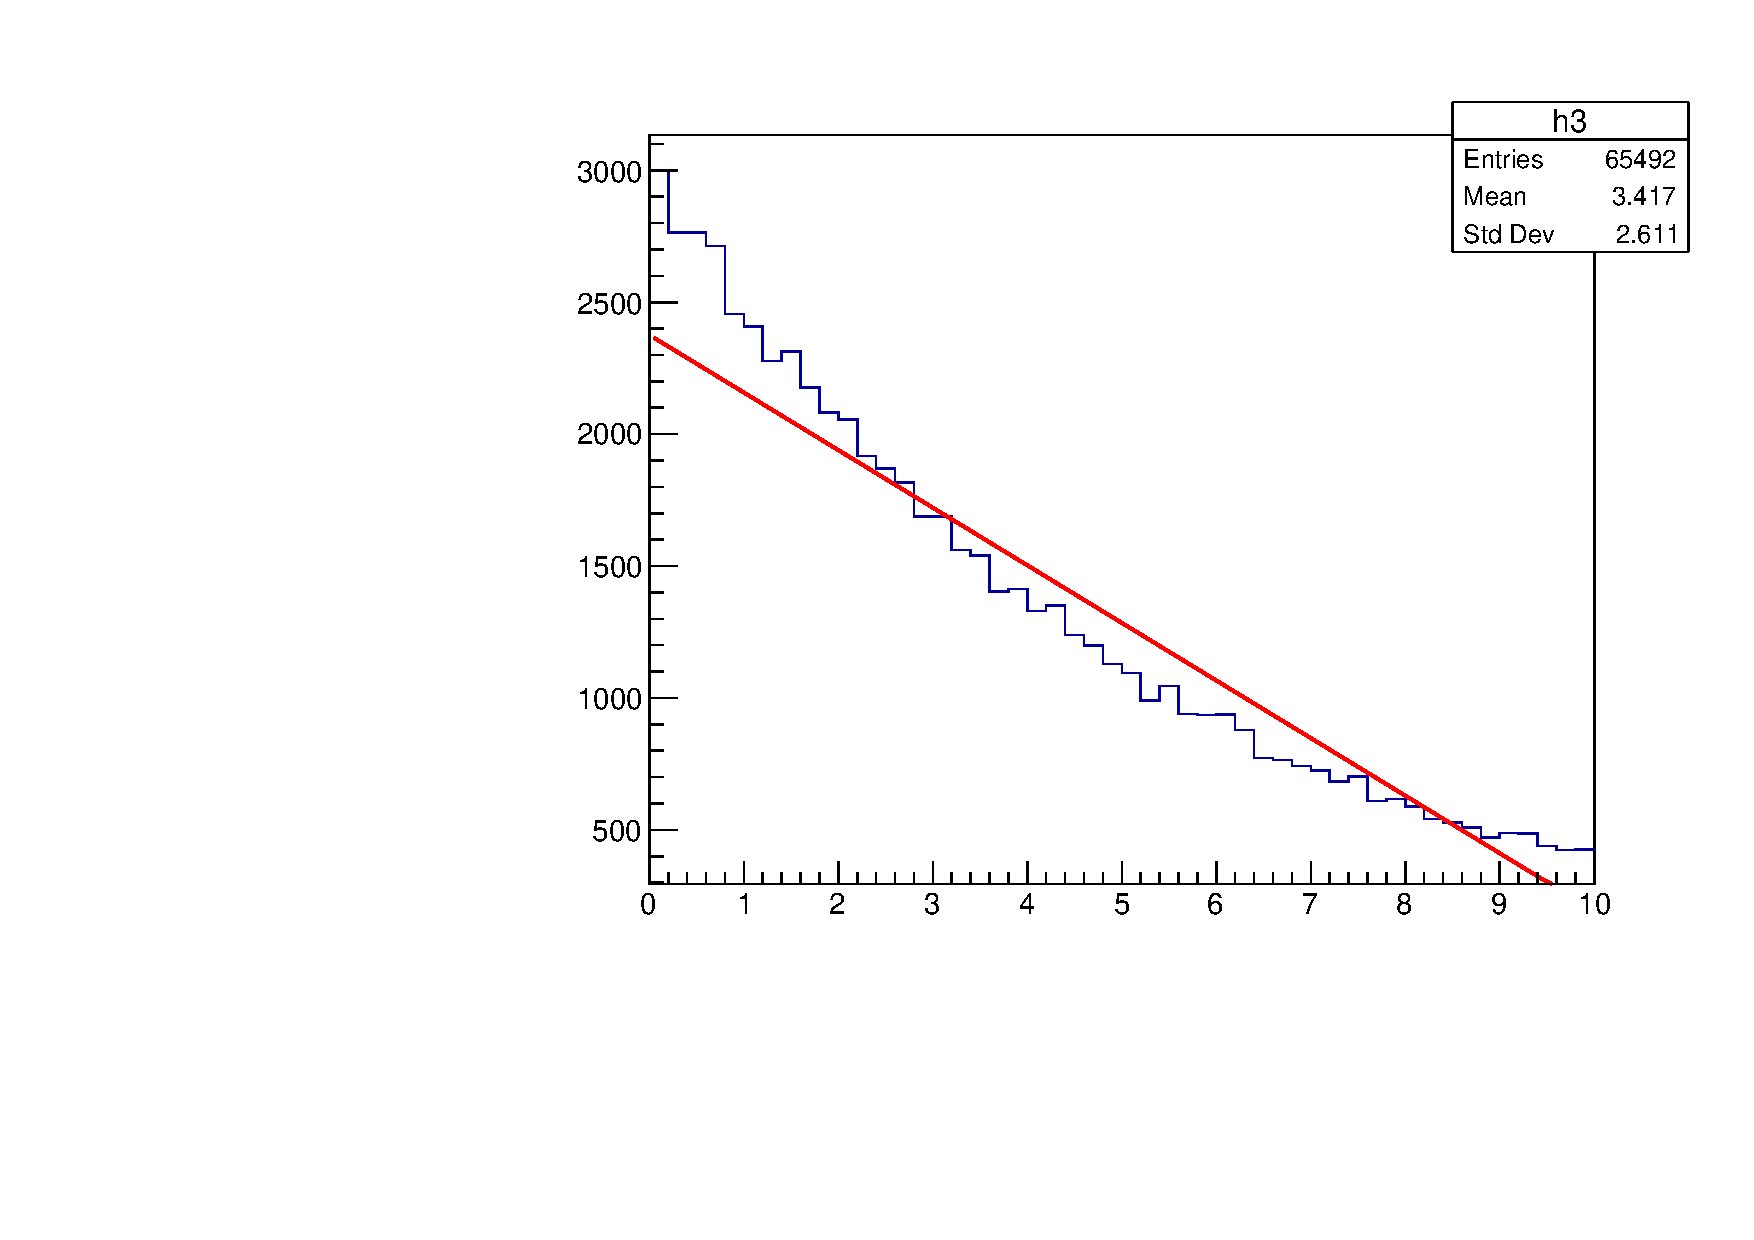
\includegraphics[scale=0.35]{Pictures/fitexpsbagliato.pdf}
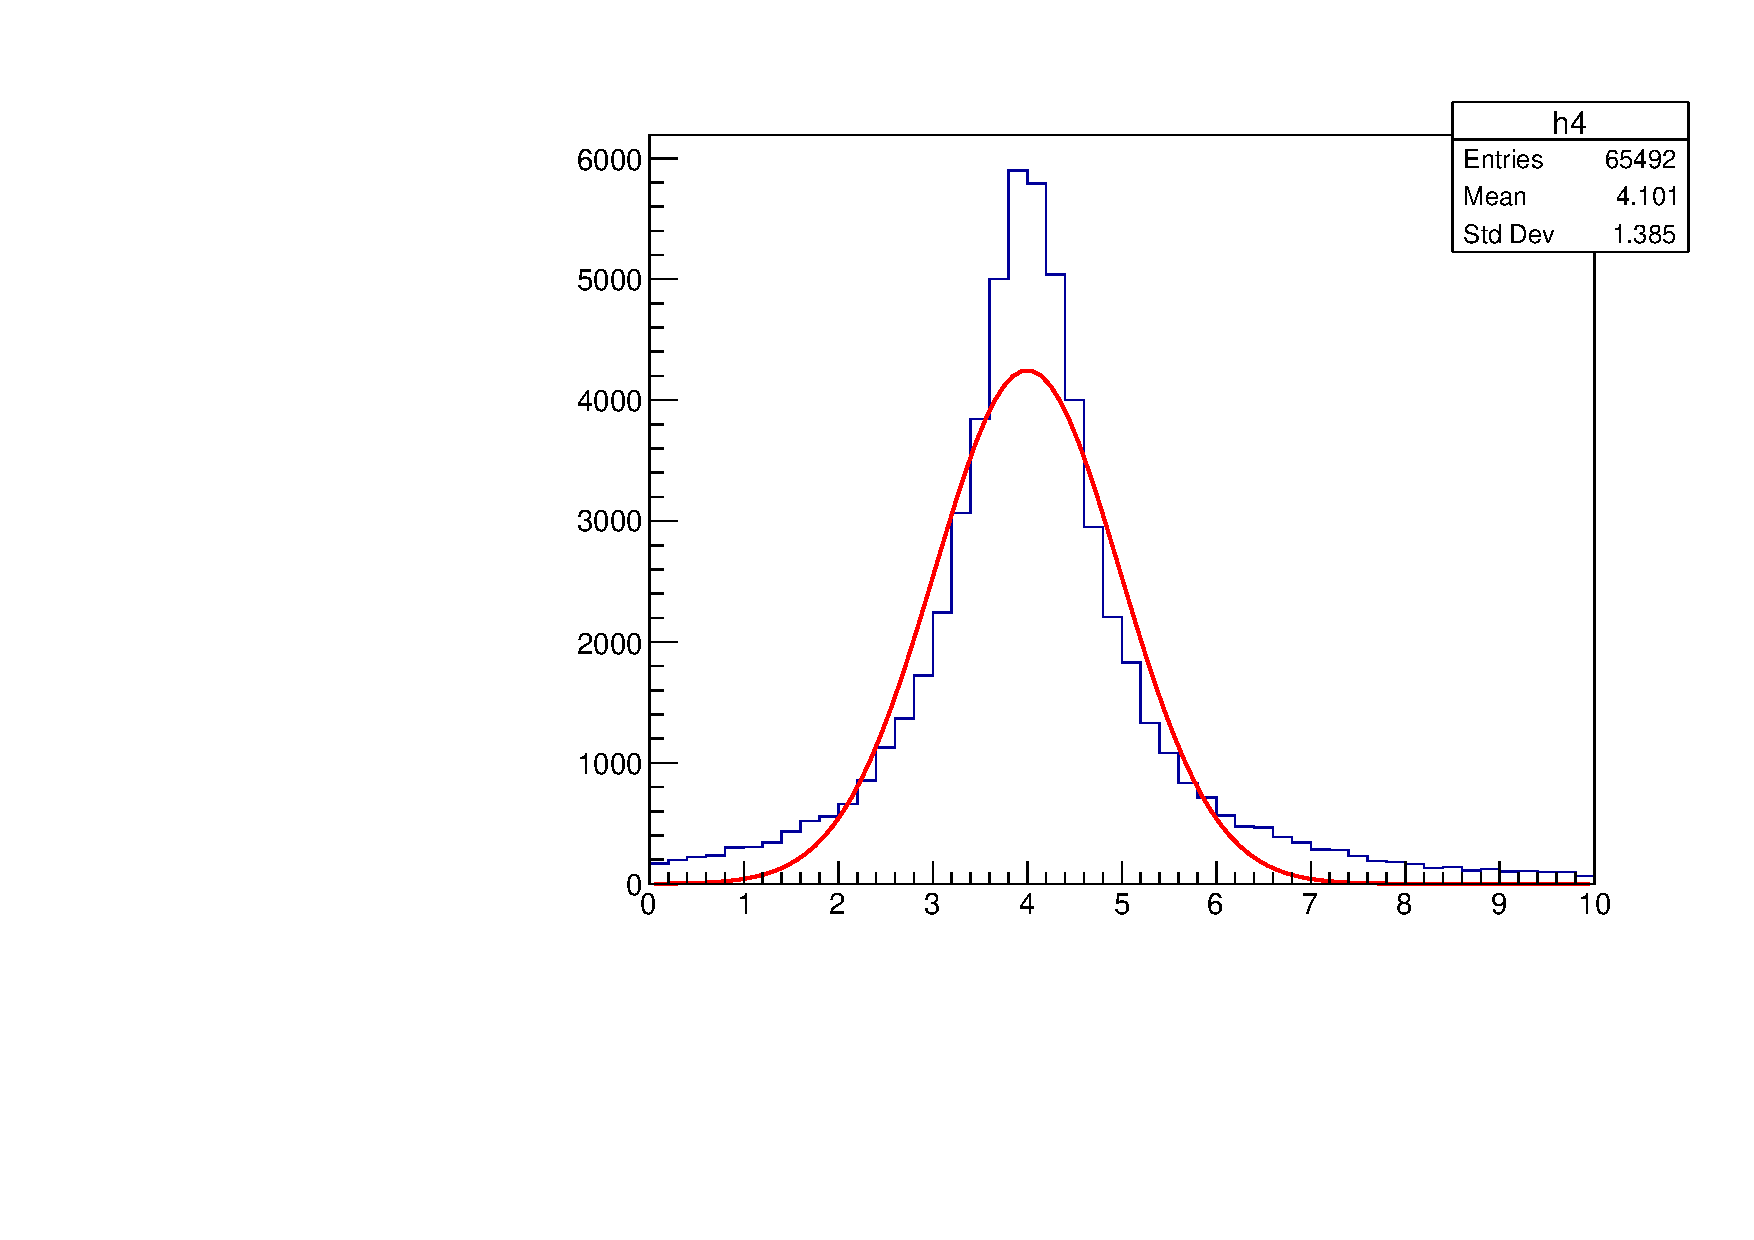
\includegraphics[scale=0.35]{Pictures/fitgaussbagliato.pdf}
\caption{A destra è rappresentato l'istogramma n.5 dei figura \ref{fig6h1} fittato con una retta, a destra l'istogramma n. 6 fittato con una Gaussiana. \label{fitbabbo2}}
\end{figure}

Osservando qualitativamente la figura \ref{fitbabbo2}, senza ricorrere al $\chi^2$ o ad altri test statistici, subito ci accorgiamo che qualcosa non va, i modelli che abbiamo scelto non funzionano, nel senso che non sono utili a rappresentare i dati.
Riproviamo a ripetere l'esercizio, utilizzando nel primo caso un polinomio di secondo grado, mentre nel secondo caso proviamo a utilizzare una funzione tipo Breit-Wigner:

$$f(x) = A\cdot \frac{\Gamma^2/4}{{(x-x_0)}^2+\Gamma^2/4}$$

che parametrizzeremo la funzione nel seguente modo:


\begin{lstlisting}[language=c++]
{
double low=0., high=10.; //gli estremi dell'intervallo di definizione della funzione
TF1 *funz = new TF1("funz","[0]/(pow(x-[1],2)+[2])",low,high);
//dove il parametro [0] rappresenta l'ampiezza, [1] il punto di massimo, [2] la semi-ampiezza.
}
\end{lstlisting}

Utilizzando i codici 
\begin{lstlisting}[language=c++]
{
histo[2]->Fit("pol2"); //usiamo la parola chiave pol2 per il polinomio di secondo grado
c1->SaveAs("fig1.pdf");
TF1 *funz = new TF1("funz","[0]/(pow(x-[1],2)+[2])",0,10);
histo[3]->Fit("funz","R"); //utilizziamo la nostra parametrizzazione
c1->SaveAs("fig2.pdf");
}
\end{lstlisting}
otteniamo le seguenti figure:

\begin{figure}[h]
\centering
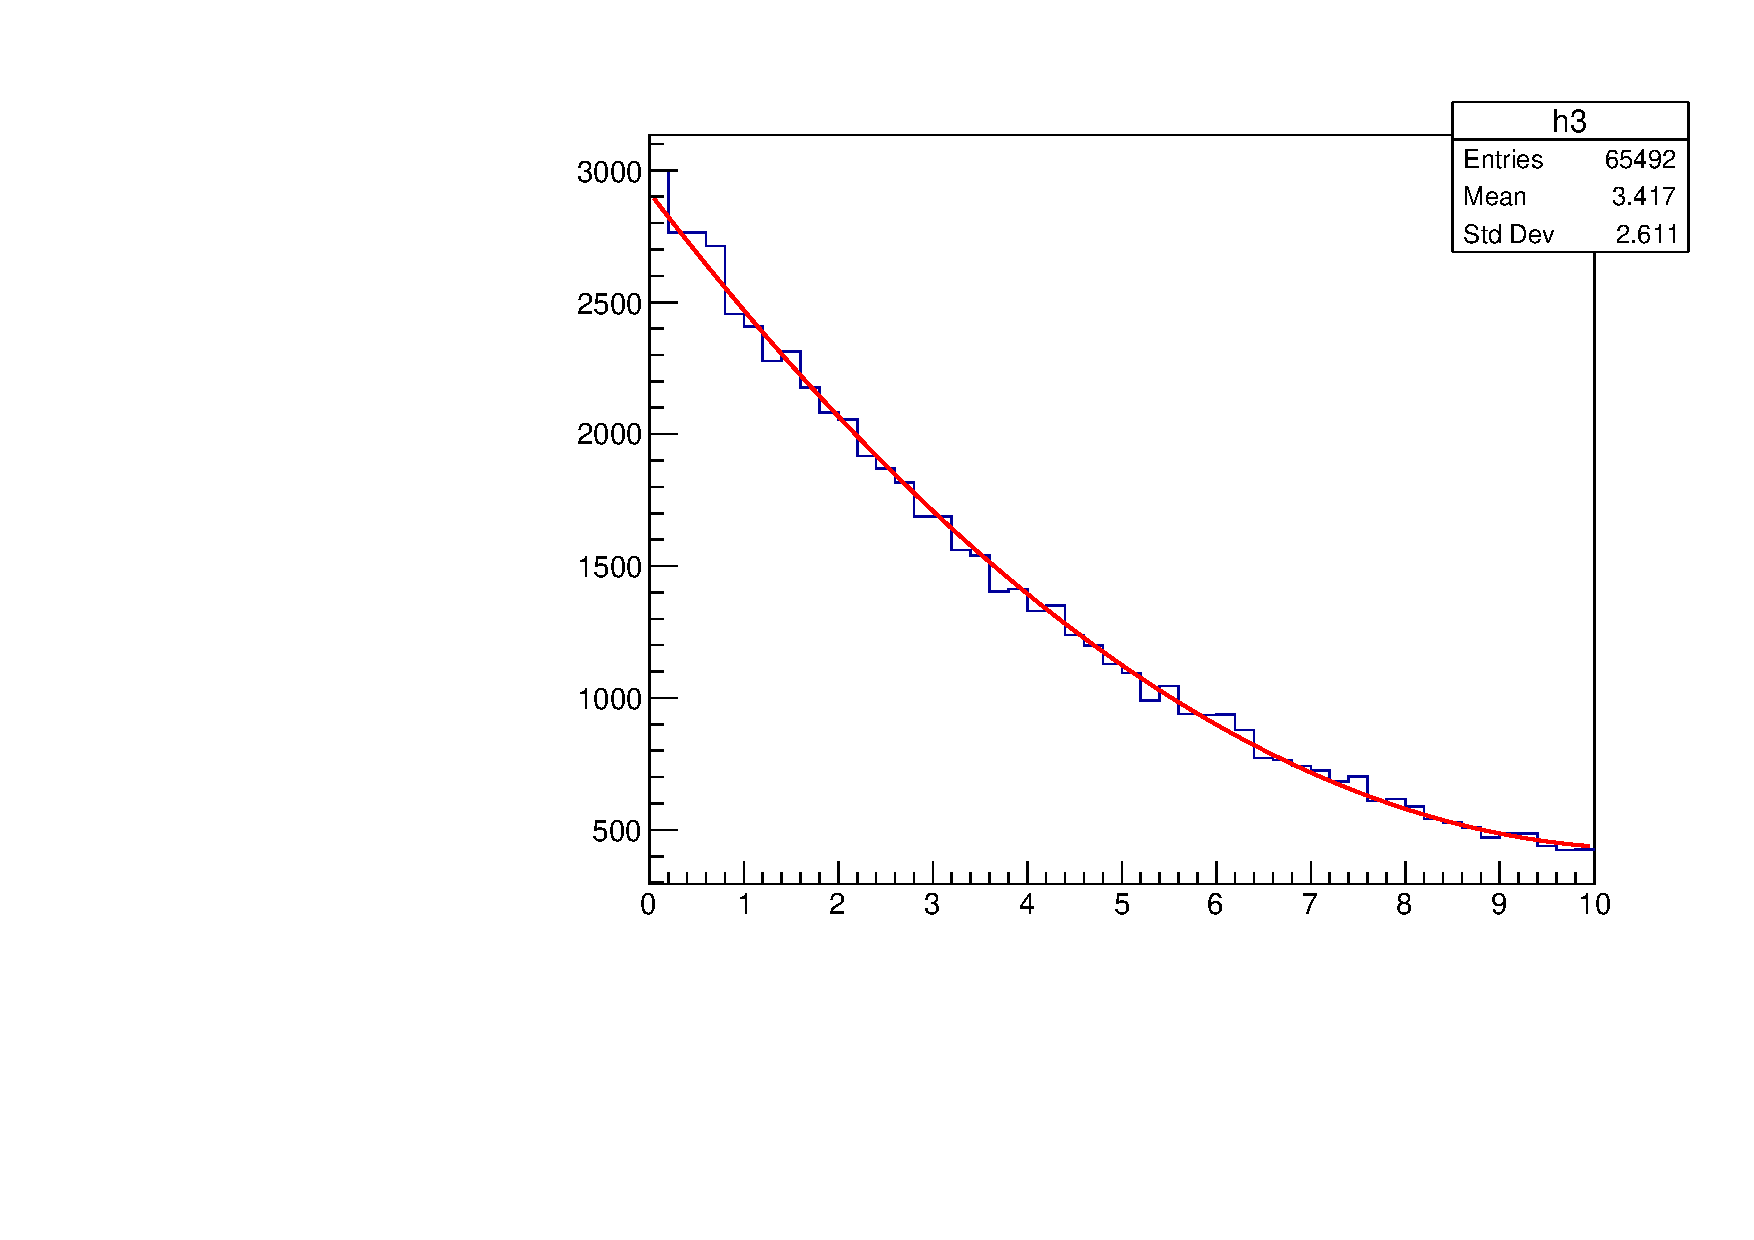
\includegraphics[scale=0.35]{Pictures/fitexpsbagliato2.pdf}
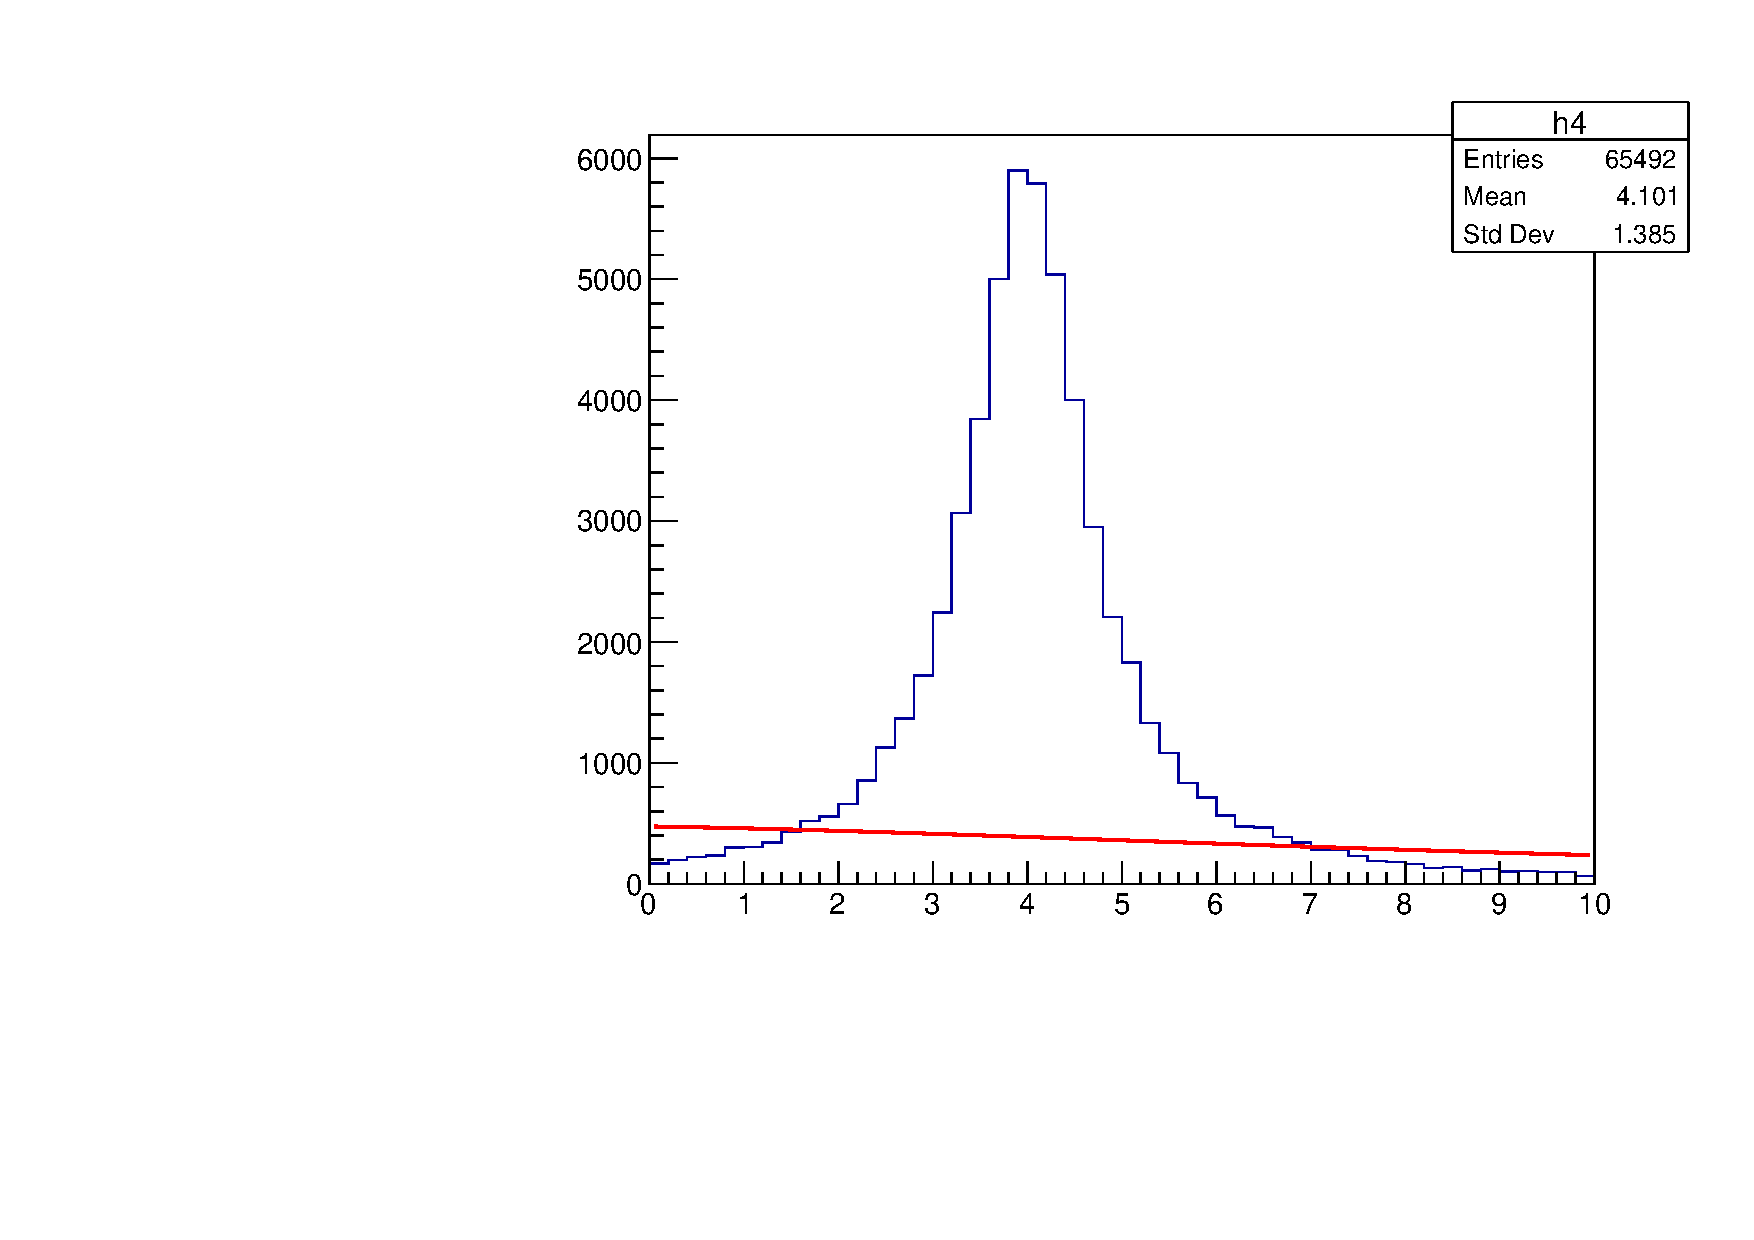
\includegraphics[scale=0.35]{Pictures/fitebwsballata.pdf}
\caption{A destra è rappresentato l'istogramma n.5 dei figura \ref{fig6h1} fittato con una parabola, a destra l'istogramma n. 6 fittato con una Breit-Wigner. \label{fitbabbo3}}
\end{figure}

In figura \ref{fitbabbo3} possiamo osservare come utilizzando un polinomio di secondo grado siamo riusciti a rappresentare bene l'andamento dell'istogramma riportato a sinistra, mentre il nostro modello sembra non essere riuscito nel compito che ci eravamo figurati nel caso dell'istogramma riportato nella figura a destra.
In realtà, il modello utilizzato per il fit della figura a sinistra non è quello corretto, infatti per generare questi dati è stata utilizzata una funzione esponenziale decrescente. L'ottimo accordo tra il modello e i dati è matematicamente accidentale, nel senso che un polinomio di secondo grado ben approssima un esponenziale e quindi non ci siamo accorti dell'incorrettezza del modello usato.
Nel secondo caso invece, il modello è corretto, quello che è andato storto non dipendeva dal modello ma dagli algoritmi di minimizzazione che lavorano dietro il processo di Fit. Questi algoritmi variano i parametri della funzione fino a trovare la migliore configurazione rispetto all'accordo con i dati, ma questo processo di ricerca non lavora all'infinito, e quindi può accadere che nello spazio delle possibili soluzioni, il sistema sia decaduto in una configurazione di minimo relativo lontano dal minimo assoluto che noi vogliamo ottenere (come nel nostro caso).
Allora in questi casi è necessario suggerire al sistema dei valori dei parametri della funzione che si avvicinano ai valori che vogliamo cercare.

Proviamo nuovamente a fare il fit, ma questa volta utilizzando il metodo \textit{SetParamenters(primoparametro,secondoparametro,ecc)} suggeriamo al fit valori prossimi a quelli corretti:

\begin{lstlisting}[language=c++]
{
//scatola per le figure
TCanvas *box = new TCanvas("box","",600,500);
//definiamo la Breit-Wigner
TF1 *funz = new TF1("funz","[0]/(pow(x-[1],2)+[2])",0,10);
//suggeriamo i parametri di innnesco del fit
funz->SetParameters(2000,4,0.5);
histo[3]->Fit("funz","R");
box->SaveAs("fitebwsgiusta.pdf");
//ripetiamo la stessa procedura per l'esponenziale
TF1 *funz2 = new TF1("funz2","[0]*exp(-[1]*x)",0,10);
funz->SetParameters(1,1);
histo[2]->Fit("funz2","R");
box->SaveAs("fitexpgiusta.pdf");
}
\end{lstlisting}
Il risultato dei codici corretti sono riportati in figura \ref{fitbabbo4}.

\begin{figure}[h]
\centering
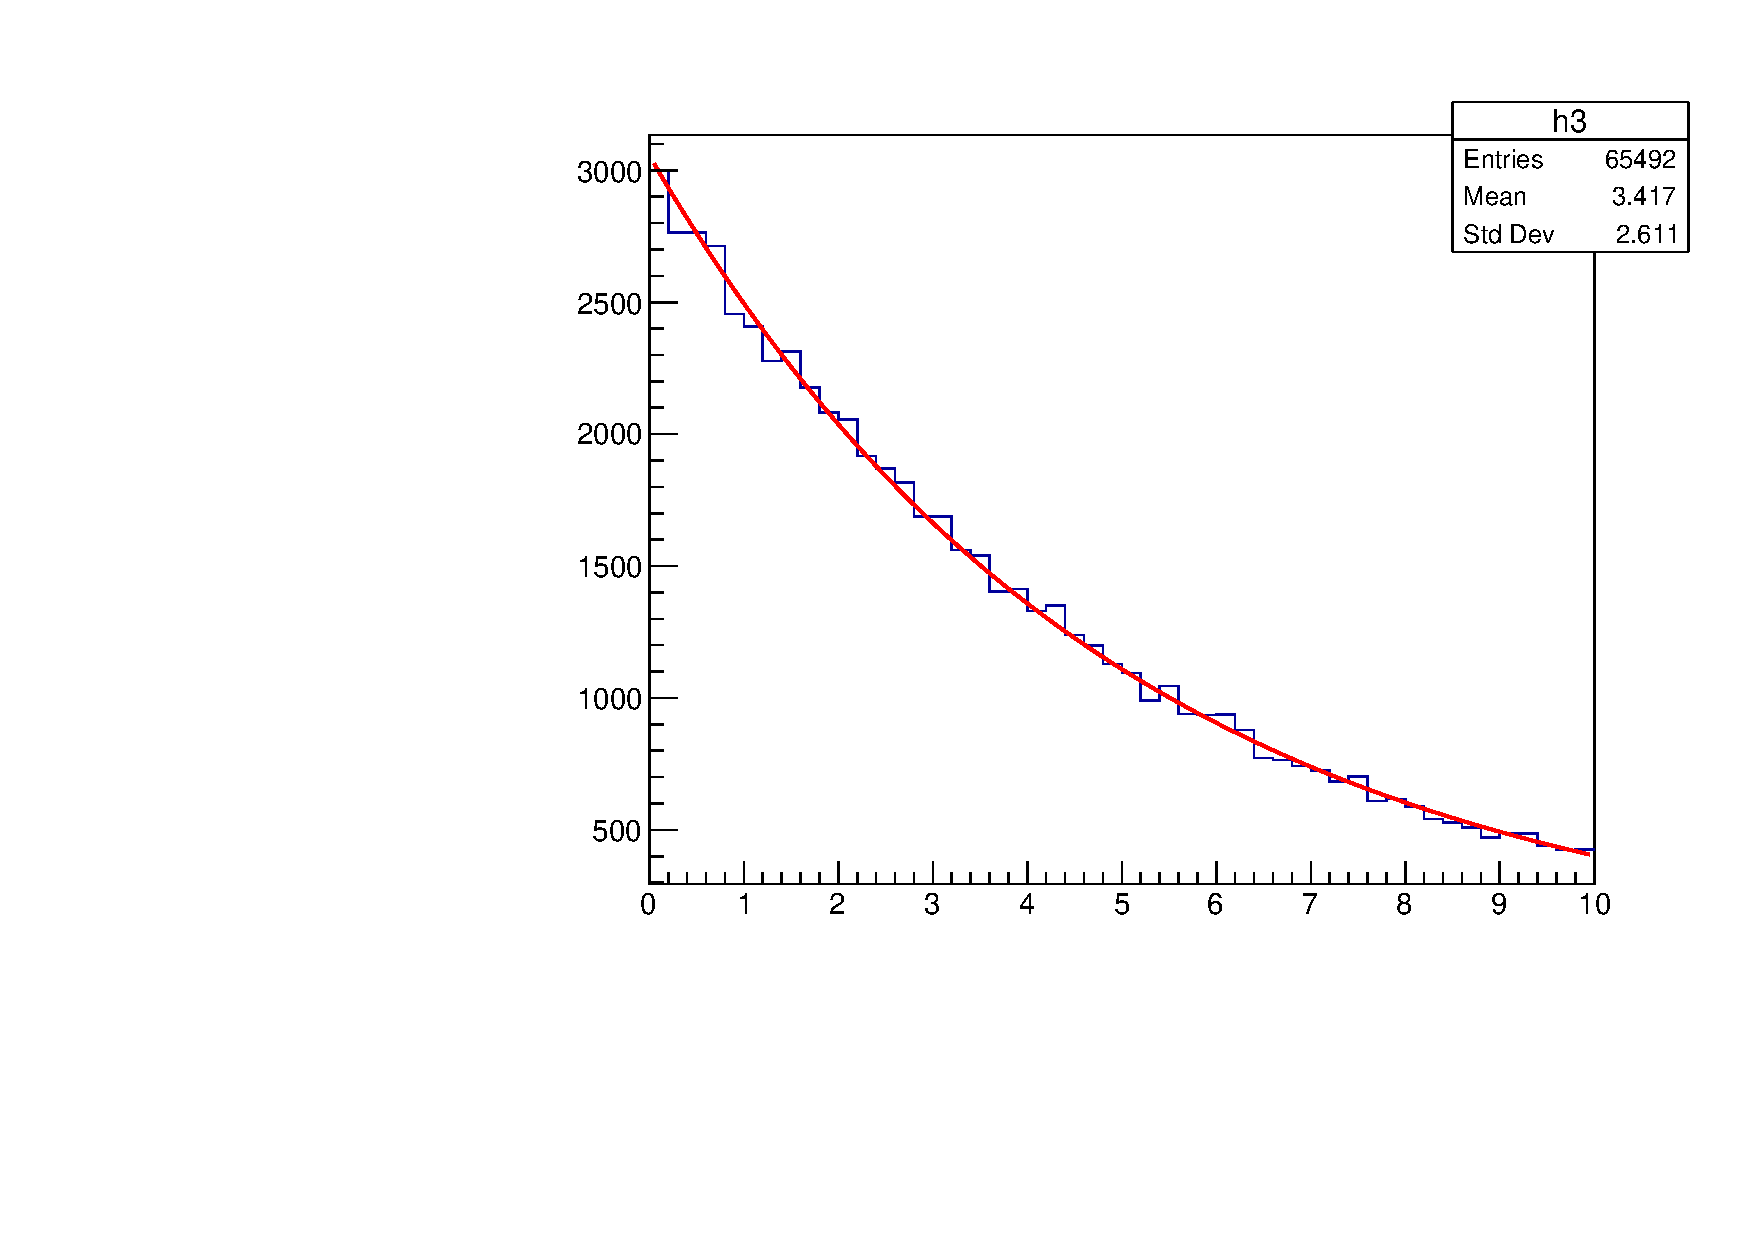
\includegraphics[scale=0.35]{Pictures/fitexpgiusta.pdf}
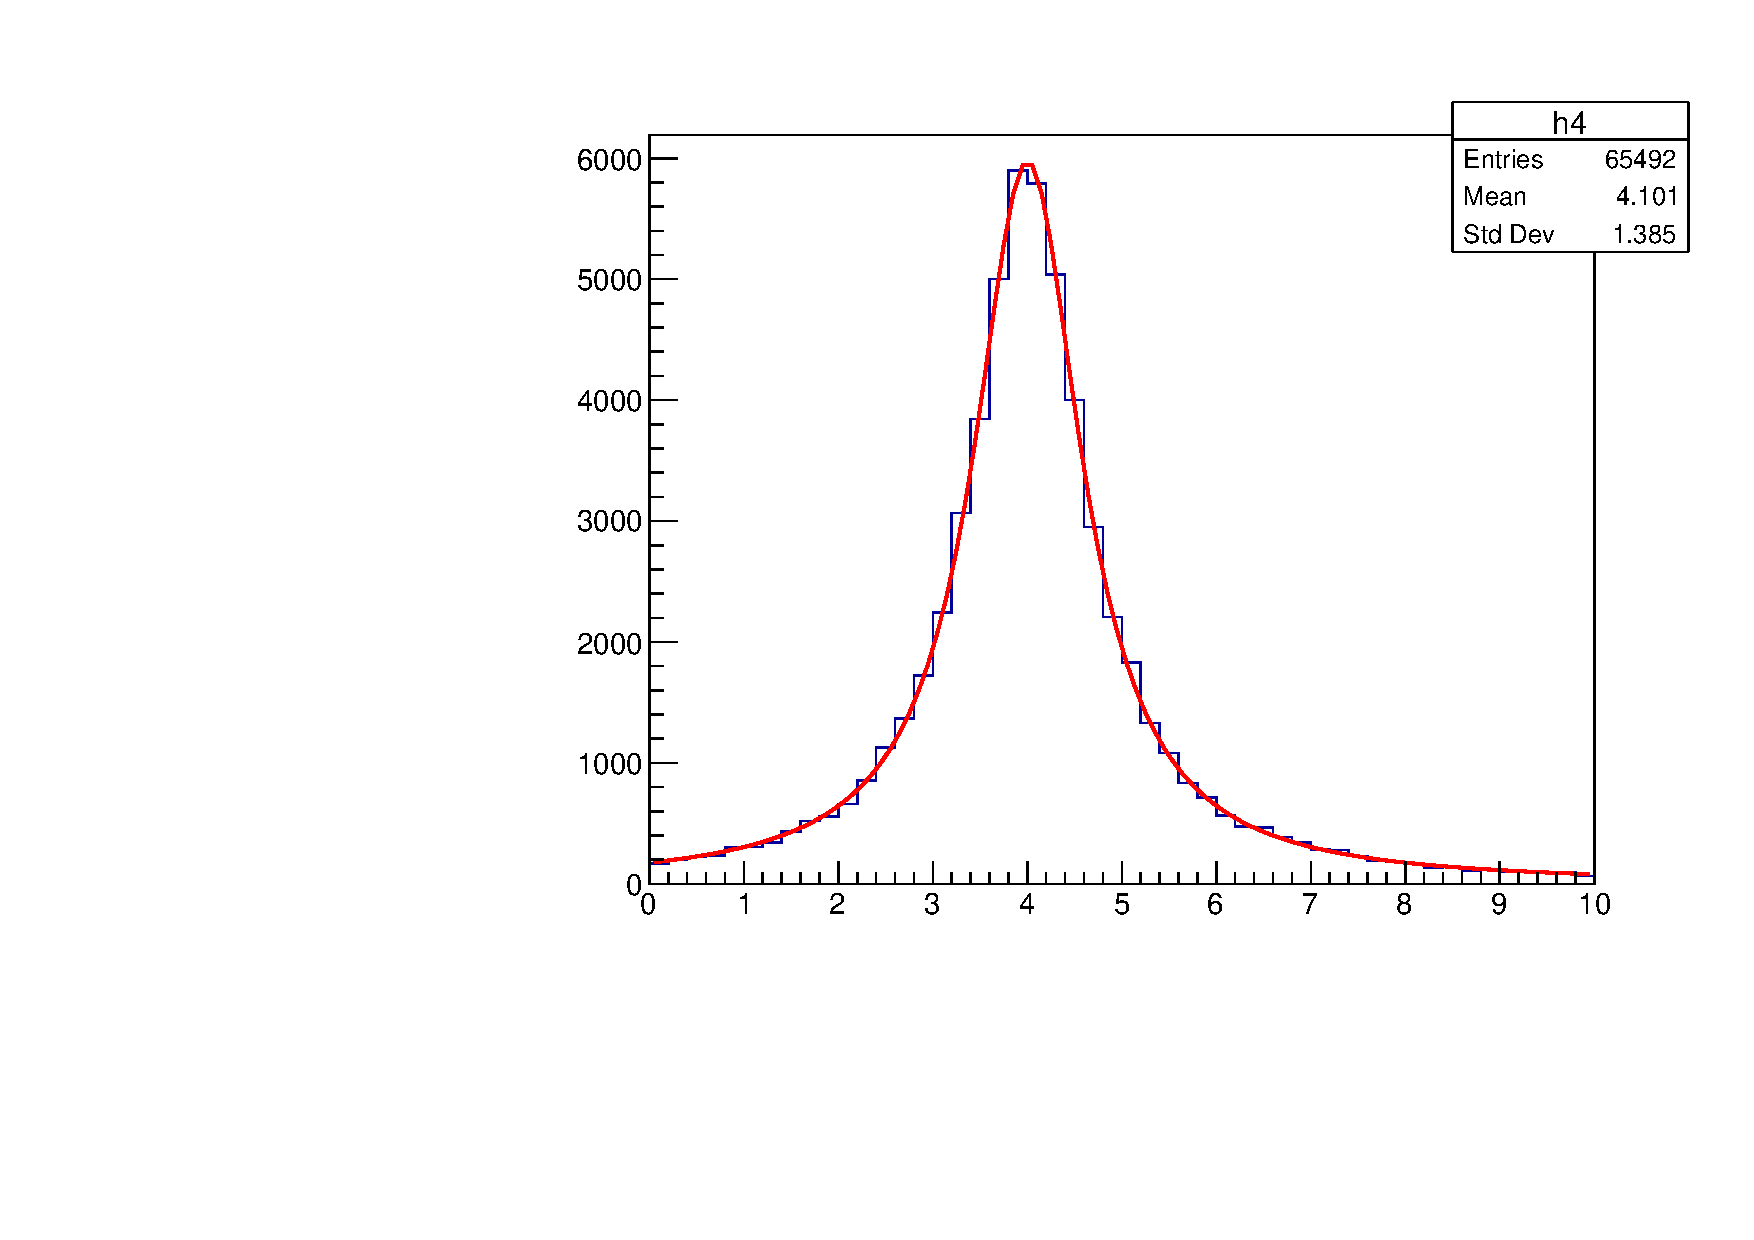
\includegraphics[scale=0.35]{Pictures/fitebwsgiusta.pdf}
\caption{A destra è rappresentato l'istogramma n.5 dei figura \ref{fig6h1} fittato con una esponenziale decrescente, a destra l'istogramma n. 6 fittato con una Breit-Wigner. In entrambi i fit sono stati suggeriti dei parametri prima di effettuare il fit. \label{fitbabbo4}}
\end{figure}
Come possiamo osservare in figura \ref{fitbabbo4}, entrambi gli istogrammi sono descritti perfettamente dai modelli proposti.
Una ulteriore riflessione potrebbe sorgere guardando il pannello di sinistra delle figure \ref{fitbabbo3} e \ref{fitbabbo4}, in entrambi i casi il fit con la parabola e con l'esponenziale decrescente riescono a descrivere bene i nostri dati, allora in questo caso a quale modello dovremmo credere? In realtà, entrambi i fit sono corretti quello che cambia è l'informazione che vogliamo estrarre dai dati. Se ad esempio sapessimo che i dati sono testimoni dell'andamento di una popolazione di nuclidi in un processo di decadimento, ebbene in questo caso il modello con l'esponenziale decrescente ci consentirebbe di estrarre una informazione fisica importante come la costante di decadimento. Quindi in conclusione la correttezza della scelta del modello da utilizzare per rappresentare i propri dati dipende da quali informazioni vogliamo estrarre e da quante cose conosciamo sulla natura dei dati che stiamo analizzando.

\section{Fit di istogrammi con forme composte}
In questo paragrafo proveremo ad effettuare il fit di un set di dati che presenta una sovrapposizione di due segnali differenti. Gli esempi più semplici con i quali possiamo iniziare potrebbero essere le prime due figure riportate in figura \ref{fig6h1}, in questi due casi già sappiamo che abbiamo la sovrapposizione di una Gaussiana e di un esponenziale decrescente nel primo istogramma, mentre abbiamo una parabola e una Breit-Wigner nel secondo.

Di seguito riportiamo un codice capace di effettuare i due fit con successo:

\begin{lstlisting}[language=c++]
{
 ifstream leggimi("daterelli2.dat");

 TH1D *hist[2];
 for(int i=0; i<2; i++)
  {
  hist[i]=new TH1D(Form("h%d",i),"",50,0,10);
  }
  double a,b;
while(sc>>a>>b)
{
	hist[0]->Fill(a);
	hist[1]->Fill(b);
}
leggimi.close();

TCanvas *grafici = new TCanvas("grafici", "", 1200,600);
grafici->Divide(2,1);

//fit dell'istogramma 1 composto da esponenziale + gaussiana
TF1 * funz1= new TF1("funz1","[0]*exp(-[1]*x)", 0,3);
funz1->SetParameters(1,1);
funz1->SetParNames("a","b"); //diamo dei nomi ai parametri in modo da evitare errori di identificazione dei parametri nella definizione della funzione somma
TF1 * funz2= new TF1("funz2","[0]*exp(-pow(x-[1],2)/[2])", 3.7,6.3);
funz2->SetParameters(1,1,1);
funz2->SetParNames("c","d","e");
funz2->SetLineColor(3);

grafici->cd(1);

hist[0]->Draw();
hist[0]->Fit("funz1","R");//R significa che il fit si limita ai dati che vivono nell'intervallo di definizione della funzione
hist[0]->Fit("funz2","R+"); //l'opzione + consente di  sovrapporre nella figura il secondo fit
//definiamo la funzione somma
//e' IMPORTANTISSIMO definire la funzione somma dopo aver effettuato i primi due fit
// in modo da far ereditare alla funzione somma i parametri ottenuti dai primi due fit parziali
TF1 * somma = new TF1("somma","funz1+funz2", 0, 10);
somma->SetLineColor(1);
hist[0]->Fit("somma","R+");

//fit dell'istogramma composto da una breit-wigner e una parabola
TF1 * fun1= new TF1("fun1","[0]/(pow(x-[1],2)+pow([2]/2,2))", 3,5);      //((x-[2])*(x-[3])+[1]/4)[0]) parametrizzazione alternativa per la Breit-Wigner
fun1->SetParameters(1,1,1,1);
fun1->SetParNames("f","g","h","i");
fun1->SetLineColor(3);
TF1 * fun2= new TF1("fun2","[0]*x*x+[1]*x+[2]", 6,10);
fun2->SetParameters(1,1,1);
fun2->SetParNames("l","m","n");
grafici->cd(2);
hist[1]->Draw();
hist[1]->Fit("fun1","R");
hist[1]->Fit("fun2","R+");
//E' FONDAMENTALE definire la somma dopo aver fatto il fit di tutte le funzioni componenti di sum
TF1 * sum = new TF1("sum","fun1+fun2", 0, 10);
sum->SetLineColor(1);
hist[1]->Fit("sum","R+");
grafici->SaveAs("fitdoppi.pdf");
}
\end{lstlisting}

\begin{figure}[h]
\centering
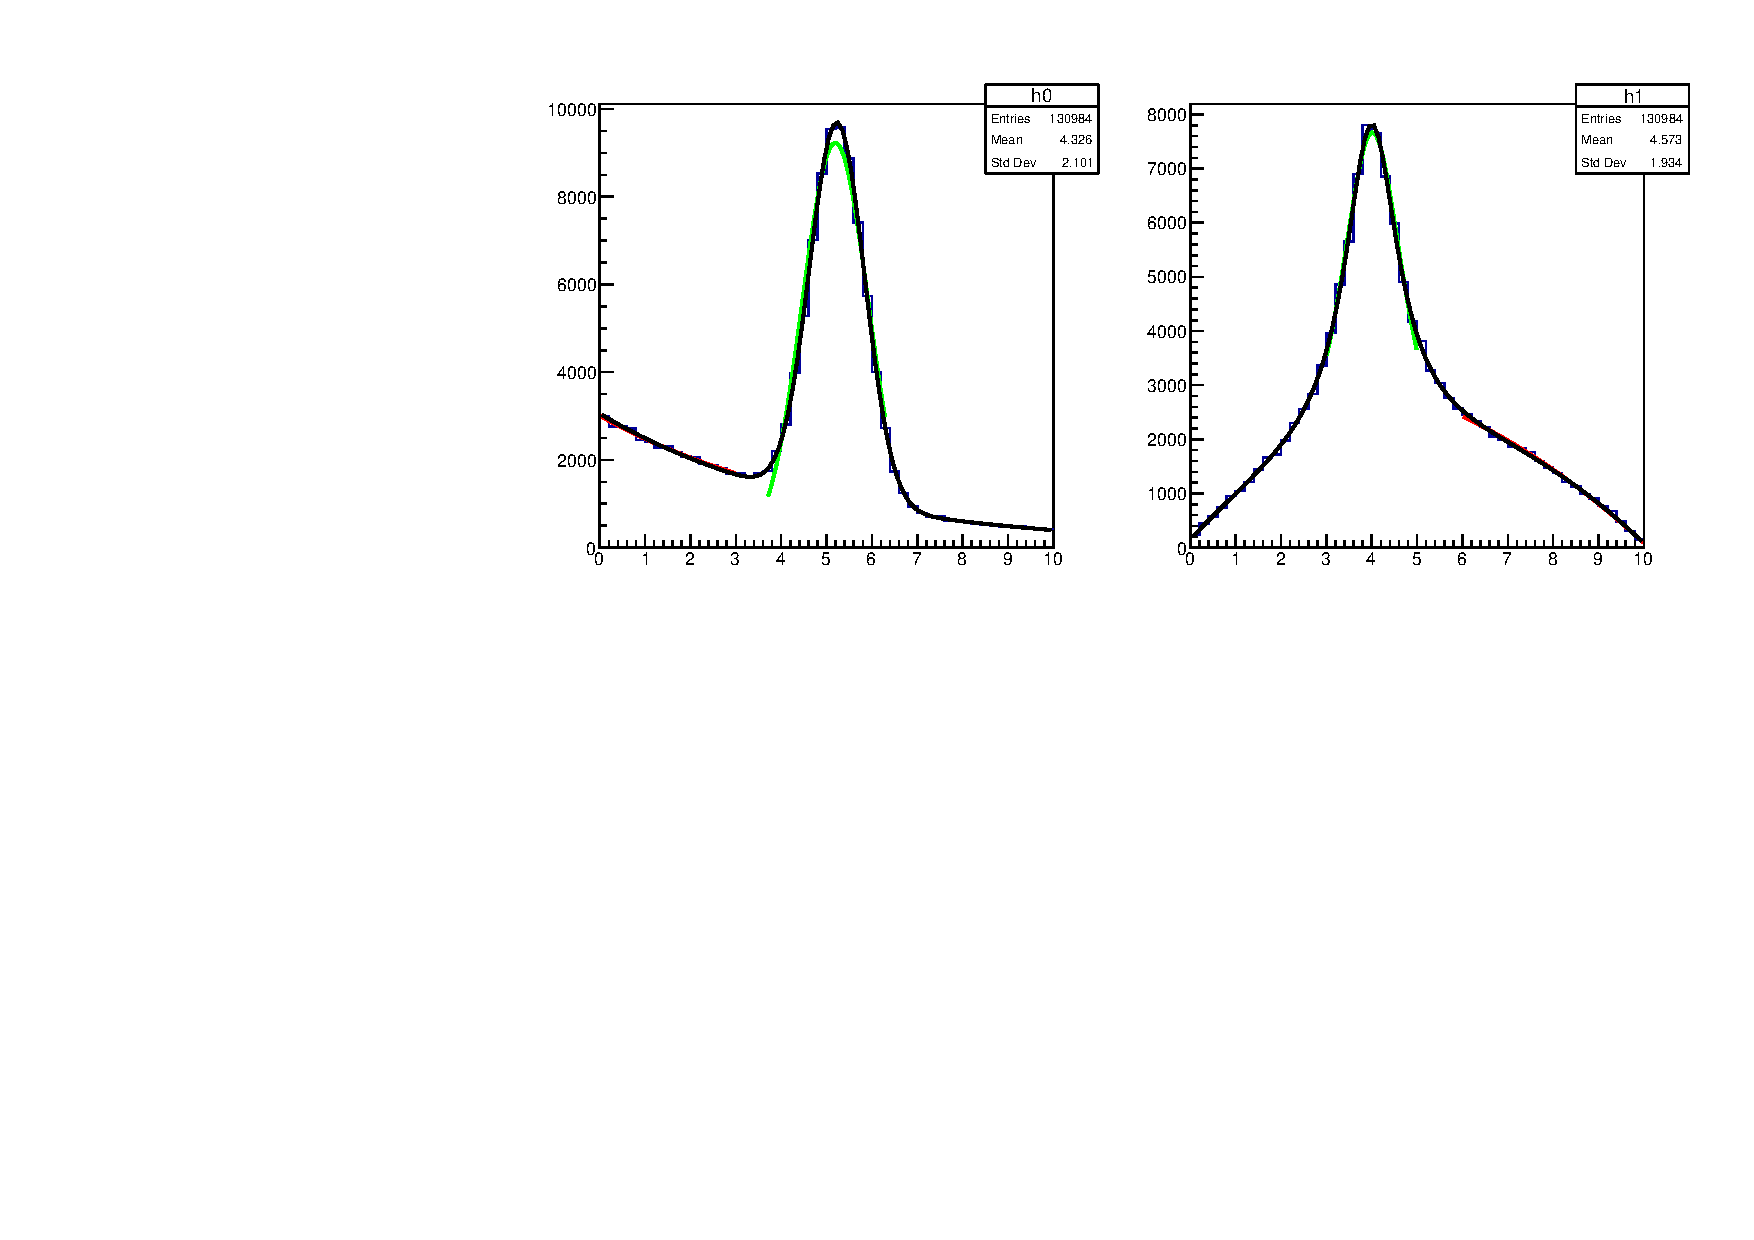
\includegraphics[scale=0.7]{Pictures/fitdoppi.pdf}
\caption{Nel pannello destro della figura è riportato il fit dell'istogramma hist[0] mentre nel pannello sinistro l'istogramma  hist[0], le curve blu indicano gli istogrammi, le curve verdi e rosse i fit componenti, mentre le curve nere il fit complessivo. \label{fitbabbo5}}
\end{figure}

Come possiamo vedere, sono stati effettuati in entrambi gli esempi, prima due fit con le funzioni componenti in regioni dove ciascuna funzione risultava dominante rispetto alla compagna. Questo è stato fatto in modo tale che i parametri ottenuti nei fit preliminari risultino quanto più prossimi possibile ai parametri definitivi della funzione composta. Una volta effettuati i fit preliminari, viene definita una funzione somma, questa volta in tutto il dominio dei dati. Facendo attenzione alla definizione dei nomi dei parametri delle funzioni componenti in modo tale che la funzione somma non faccia confusione nel riconoscerli, la funzione somma automaticamente  utilizzerà i valori dei parametri ottenuti dai fit preliminari come quantità di innesco del fit globale. Risultato finale del fit è la perfetta rappresentazione dei dati con la funzione composta.
In figura possiamo osservare in verde e in rosso i fit componenti, mentre in nero il fit globale con la funzione somma.

A questo punto, la funzione somma dopo che il fit globale è stato eseguito con successo detiene i parametri corretti delle funzioni componenti. Notiamo che le funzioni componenti sono state definiti in sotto intervalli della variabilità in cui vive l'istogramma e la funzione somma. Quindi se volessimo produrre una figura in cui rappresentiamo il fit globale e l'andamento delle funzioni componenti, dovremmo correggere il range di variabilità delle funzioni componenti estendendolo a tutto l'intervallo di variabilità dei dati, e inoltre bisognerà trovare il modo di trasferire i parametri estratti dalla funzione somma alle funzioni componenti:
\begin{lstlisting}[language=c++]
{
 ifstream sc("daterelli2.dat");
 TH1D *hist=new TH1D("hist","",50,0,10);
 double a,b;
 while(sc>>a>>b)
 {
	hist->Fill(b);
 }

 //fit dell'istogramma 6 composto da breit-wigner e parabola
 TF1 * fun1= new TF1("fun1","[0]/(pow(x-[1],2)+pow([2]/2,2))", 3,5);      //((x-[2])*(x-[3])+[1]/4)[0]) altra forma della breit
  fun1->SetParameters(1,1,1,1);
  fun1->SetParNames("f","g","h","i");
  fun1->SetLineColor(3);
  TF1 * fun2= new TF1("fun2","[0]*x*x+[1]*x+[2]", 6,10);
  fun2->SetParameters(1,1,1);
  fun2->SetParNames("l","m","n");

 TCanvas * pippo = new TCanvas("pippo","",600,500);

  hist->Draw();
//cloniamo l'istogramma di lavoro in modo da conservare una copia pulita
//non sporcata dai processi di fit (e' solo una finezza grafica)
TH1D *pino = (TH1D*)hist->Clone();
//effettuiamo i fit delle funzioni componenti
hist->Fit("fun1","R");
hist->Fit("fun2","R+");
//E' FONDAMENTALE definire la somma dopo aver fatto il fit con fun1 e fun2
//sum eredita i parametri dei fit preliminari automaticamente
TF1 * sum = new TF1("sum","fun1+fun2", 0, 10);
sum->SetLineColor(1);
//fit globale con la funzione somma
hist->Fit("sum","R+");
//contenitore per copiare i parametri dopo il fit globale
double parametri[6];
//metodo per copiare in un solo colpo tutti i parametri
sum->GetParameters(parametri);
//sum->GetParameters(&parametri[0]); //comando equivalenti, in questo caso specifichiamo da quale elemento deve partire a copiare
//IMPORTANTISSIMO->Correggiamo l'intervallo di definizione delle funzioni componenti
fun1->SetRange(0,10);
fun2->SetRange(0,10);
//passiamo alle componenti i parametri ottenuti con il fit globale
fun1->SetParameters(&parametri[0]);
fun2->SetParameters(&parametri[3]);
pino->Draw();
//sovrapponiamo al grafico pulito le funzioni somma e componenti
sum->Draw("same");
fun1->Draw("same");
fun2->Draw("same");
pippo->SaveAs("fitsecondo.pdf");
}
\end{lstlisting}

Il risultato di questo codice è riportato nella seguente figura \ref{fitbabbo6}.

\begin{figure}[h]
\centering
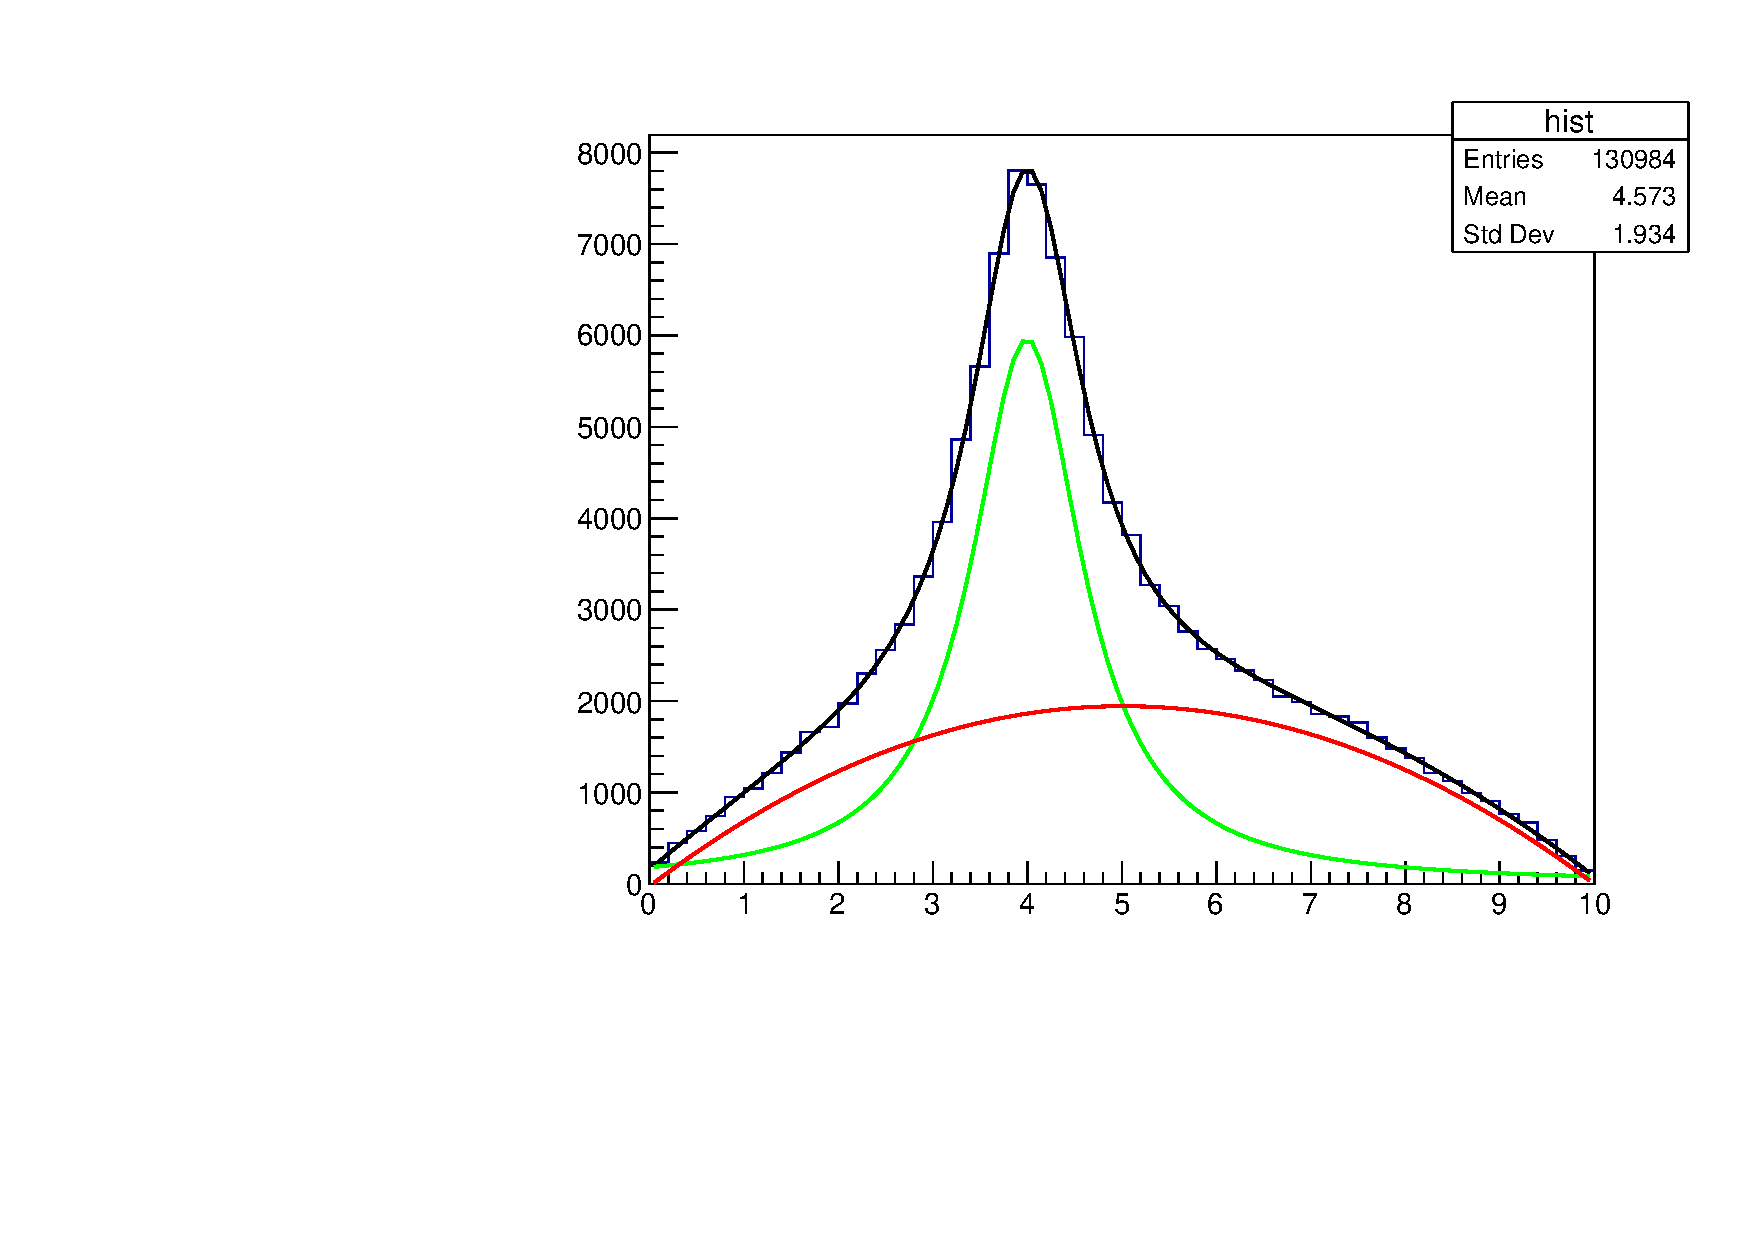
\includegraphics[scale=0.5]{Pictures/fitsecondo.pdf}
\caption{In blu è rappresentato l'istogramma, in nero il fit globale, in rosso e verde le funzioni componenti con i parametri prodotti dal fit globale. \label{fitbabbo6}}
\end{figure}

\section{Riconoscimento del fondo e sottrazione del fondo}

Il codice che segue fino alla riga 67 produce le condizioni che hanno consentito di mettere in grafico la figura \ref{fitbabbo6}, la parte interessante arriva alla riga 69, dove con il semplice metodo \textit{Add} utilizziamo la funzione espo con i parametri corretti del fit globale e con i range ridefinito in tutto l'intervallo di definizione dell'istogramma, per sottrarre all'istogramma copia2, ottenuto come clone dell'istogramma originale  \textit{istogramma} attraverso il metodo Clone(), i conteggi imputati al fondo espo e conputati come il valore della funzione nel punto medio di ciascun bin. In altra parole, con la riga 69, chiediamo di sottrarre all'istogramma copia2 bin-a-bin il valore della funzione calcolata nel centro del bin.
\begin{lstlisting}[language=c++]
{
		TCanvas *finestra = new TCanvas("finestra", "finestra",600, 500);
		ifstream dati1x("dati1x.dat");
		TH1D *istogramma = new TH1D("Istogramma", "", 100, 0,20);
		double a;
		while(dati1x>>a){
			istogramma->Fill(a);
		}
		istogramma->Draw();
		//creiamo una copia dell'istogramma originale
		TH1D *copia1 = (TH1D*)istogramma->Clone();
        TH1D *copia2 = (TH1D*)istogramma->Clone();
        //definiamo le funzioni componenti
		TF1 *espo = new TF1("espo", "[0]*exp(-x/[1])", 4,10);
		espo->SetParameters(1,1);
		espo->SetParNames("Aparametro","Bparametro");

		TF1 *bww = new TF1 ("bww", "[0]/(pow(x-[1],2)+pow([2]/2, 2))", 1,3.5);
		bww->SetParameters(1,1,1);
		bww->SetParNames("Cparametro","Dparametro","Eparametro");

		TF1 *bww2 = new TF1 ("bww2", "gaus", 13,15);
		bww2->SetParameters(1,1,1);
		bww2->SetParNames("Fparametro","Gparametro","Hparametro");

		TF1 *gaussiana = new TF1 ("gaussiana", "gaus", 11.5,13);
		gaussiana->SetParameters(1,1,1);
		gaussiana->SetParNames("Iparametro","Lparametro","Mparametro");

		istogramma->Fit("espo", "R");
		istogramma->Fit("bww", "R+");
		istogramma->Fit("bww2", "R+");
		istogramma->Fit("gaussiana", "R+");
        //dopo aver effettuato il fit delle componenti definiamo la funzione somma
		TF1 *funzione_somm = new TF1("funzione_somma", " espo + bww + bww2 + gaussiana", 0, 20);
		funzione_somm->SetLineColor(1);

		istogramma->Fit("funzione_somma", "R+");
        //estraiamo dalla funzione somma dei parametri statistici fondamentali
		double aaaa = funzione_somm->GetNDF();
		double bbbb = funzione_somm->GetChisquare();
		double cccc = funzione_somm->GetProb();

		cout<<"Gradi di liberta': "<<aaaa<<" ChiQuadro: "<<bbbb<<" Prob: "<<cccc<<endl;
		cout<<"Il chi quadro ridotto e': "<<bbbb/aaaa<<endl;

		double parametriii[11];
		//estraiamo dalla funzione somma i parametri del fit globale
		funzione_somma->GetParameters(parametriii);
		for (int i=0; i<11;i++)cout<<parametriii[i]<<endl;
		TCanvas *finestrella = new TCanvas("finestrella", "finestrella",600, 500);
        //mettiamo a grafico la prima copia
		copia1->Draw();

		funzione_somma->GetParameters(parametriii);
        //trasferiamo alle funzioni componenti i parametri del fit globale
		espo->SetParameters(&parametriii[0]);
		bww->SetParameters(&parametriii[2]);
		bww2->SetParameters(&parametriii[5]);
		gaussiana->SetParameters(&parametriii[8]);
		//Modifichiamo il range di definizione delle funzioni componenti
		espo->SetRange(0,20);
		bww->SetRange(0,20);
		bww2->SetRange(0,20);
		gaussiana->SetRange(0,20);
        //Effettuiamo la sottrazione del fondo!!!!!!tataaaaaaa
        
        copia2->Add(espo,-1);
		copia2->Draw("same");
		//mettiamo a grafico le componenti
		espo->Draw("same");
		bww->Draw("same");
		bww2->Draw("same");
		gaussiana->Draw("same");

}
\end{lstlisting}





\chapter{Esercizi - in progress}\index{Esercizi}

\section*{}
In questo capitolo saranno riportati tutti gli esercizi che sono stati proposti negli esami del corso.
Molti esercizi richiedono operazioni di input/output su file che vengono forniti ai candidati durante gli esami. Questi file saranno caricati nella stessa pagina web in cui è possibile scaricare questa raccolta di appunti.



\section{Anno 2017}\index{Anno 2017}

\textbf{Compito 1}

\begin{verbatim}
1) Descrivere che compito esegue il seguente frammento di codice. (fino a 3 punti)

   int i;
   int accumulatore=0;
   for(i=0; i<1000; i++){
      accumulatore+ = i*i;
     cout<<i<<”  “<<accumulatore<<endl;
    }
    cout<<accumulatore<<endl;

2) Scrivere un codice fortran funzionante, capace di chiedere ad un
 utente due numeri reali e che ne restituisce la somma, la differenza
  e il prodotto; (fino a 4 punti)

3) Scrivere un codice C++ capace:
     a) di stampare a schermo la terza colonna del file
      “dati_compito_primasessione.dat”, 
         (fino a 2 punti)
     b) di stampare a schermo la media e la deviazione standard dei
      dati nella 5 colonna,
         (fino a 3 punti)
     c) di mettere salvare in un file “ordinato.dat” la seconda
      colonna in ordine crescente.
         (fino a 2 punti)

4) Convertire i codici del punto 3) in script root (fino a 3 punti)

5) Scrivere uno script  root capace di stampare l’istogramma della
quarta colonna del file “dati_compito_primasessione.dat” (fino a 4 punti)

6)  Scrivere una macro root capace di fare il fit Gaussiano
 dell’istogramma messo a grafico al punto 5 (fino a 3 punti)

7)  Scrivere una macro root capace di mettere a grafico 
la funzione sin(x)+cos^2(x) tra 0 e 1 (fino a 4 punti)

8) Scrivere un codice capace di calcolare l’integrale della funzione
 definita al punto 7) tra 0 e 0.5, con il metodo dei rettangoli. 
 (fino a 3 punti)

9) Scrivere una classe che richiede come informazioni due numeri reali
 e che abbia implementati i metodi per acquisire i numeri e per 
 fornire, la somma, la sottrazione, il prodotto, il logaritmo del
  primo numero moltiplicato per il secondo numero. (fino a 4 punti)
\end{verbatim}

\textbf{Compito 2}

\begin{verbatim}
1) Descrivere che compito esegue il seguente frammento di codice.
 (fino a 3 punti)

   double funzione(double x){
       if (x<0){
             return  pow(x,2);
                }
         if (x<1){
              return  x;
            }
          return 1/x;
      } 

2) Scrivere un codice fortran funzionante, capace di salvare in un
 file la serie dei numeri da zero a 100, quelli pari su una colonna e 
 quelli dispari su un’altra colonna adiacente; (fino a 4 punti)

3) Scrivere un codice C++ capace:
     a) di stampare a schermo la quinta colonna del file 
     “dati_compito_primasessione.dat”, 
         (fino a 2 punti)
     b) di stampare a schermo la media e la deviazione standard dei 
     dati nella seconda colonna,
         (fino a 3 punti)
     c) di mettere salvare in un file “ordinato.dat” la settima 
     colonna in ordine crescente.
         (fino a 2 punti)

4) Convertire i codici del punto 3) in script root (fino a 3 punti)

5) Scrivere uno script  root capace di stampare l’istogramma della 
prima colonna del file “dati_compito_primasessione.dat” (fino a 4 
punti)

6)  Scrivere una macro root capace di fare il fit Gaussiano 
dell’istogramma messo a grafico al punto 5 (fino a 3 punti)

7)  Scrivere una macro root capace di mettere a grafico la funzione 
sin2(x)+cos(x) tra 0 e 1 (fino a 4 punti)

8) Scrivere un codice capace di calcolare l’integrale della funzione 
definita al punto 7) tra 0 e 0.5, con il metodo dei rettangoli. (fino 
a 3 punti)

9) Scrivere una classe che richiede come informazioni due numeri reali 
e che abbia implementati i metodi per acquisire i numeri e per 
fornire, la somma, la sottrazione, il prodotto, il logaritmo del primo 
numero moltiplicato per il secondo numero. (fino a 4 punti).
\end{verbatim}


\textbf{Compito 3}

\begin{verbatim}
1) Descrivere che compito esegue il seguente frammento di codice. (fino a 3 punti)

      int mario = 1000;
       while(mario>0){
           if((mario%2)==0){
          cout<<mario<<endl;
          }
          mario--;
       }

2) Scrivere un codice fortran funzionante, capace stampare a schermo 
per dieci valori equidistanti tra 0 e pi-greco di x il valore di 
sin(x); (fino a 4 punti)

3) Scrivere un codice C++ capace:
     a) di stampare a schermo l’ottava colonna del file 
     “dati_compito_primasessione.dat”, 
         (fino a 2 punti)
     b) di stampare a schermo la media e la deviazione standard dei 
     dati nella sesta colonna,
         (fino a 3 punti)
     c) di mettere salvare in un file “ordinato.dat” la seconda 
     colonna in ordine crescente.
         (fino a 2 punti)

4) Convertire i codici del punto 3) in script root (fino a 3 punti)

5) Scrivere uno script  root capace di stampare l’istogramma della 
seconda colonna del file “dati_compito_primasessione.dat” (fino a 4 
punti)

6)  Scrivere una macro root capace di fare il fit Gaussiano 
dell’istogramma messo a grafico al punto 5 (fino a 3 punti)

7)  Scrivere una macro root capace di mettere a grafico la funzione 
ln(x+1) tra 0 e 1 (fino a 4 punti)

8) Scrivere un codice capace di calcolare l’integrale della funzione 
definita al punto 7) tra 0 e 1, con il metodo dei rettangoli. (fino a 
3 punti)

9) Scrivere una classe che richiede come informazioni due numeri reali 
e che abbia implementati i metodi per acquisire i numeri e per 
fornire, la somma, la sottrazione, il prodotto, il logaritmo del primo 
numero moltiplicato per il secondo numero. (fino a 4 punti).
\end{verbatim}

\textbf{Compito 4}

\begin{verbatim}
1) Descrivere che compito esegue il seguente frammento di codice. (fino a 3 punti)

      double  maria = 0.;
       for(int i=0; i<60000;i++){
           if(vettore(i)>maria){
           maria = vettore(i);
          }
        }
        cout<<”il valore ????? è”<<maria<<endl;
     Che parola bisognerebbe sostituire ai punti interrogativi?

2) Scrivere un codice fortran funzionante, che chiede ad un utente 
dieci numeri reali e dopo averli acquisiti li stampa a schermo in 
ordine decrescente; (fino a 4 punti)

3) Scrivere un codice C++ capace:
     a) di stampare a schermo la terza colonna del file 
     “dati_compito_primasessione.dat”, 
         (fino a 2 punti)
     b) di stampare a schermo la media e la deviazione standard dei 
     dati della seconda colonna,
         (fino a 3 punti)
     c) di mettere salvare in un file “ordinato.dat” la settima 
     colonna in ordine crescente.
         (fino a 2 punti)

4) Convertire i codici del punto 3) in script root (fino a 3 punti)

5) Scrivere uno script  root capace di stampare l’istogramma della 
prima colonna del file “dati_compito_primasessione.dat” (fino a 4 
punti)

6)  Scrivere una macro root capace di fare il fit Gaussiano 
dell’istogramma messo a grafico al punto 5 (fino a 3 punti)

7)  Scrivere una macro root capace di mettere a grafico la funzione 
x2+x+1 tra 2 e 5 (fino a 4 punti)

8) Scrivere un codice capace di calcolare l’integrale della funzione 
definita al punto 7) tra 0 e 1, con il metodo dei rettangoli. (fino a 
3 punti)

9) Scrivere una classe che richiede come informazioni due numeri reali 
e che abbia implementati i metodi per acquisire i numeri e per 
fornire, la somma, la sottrazione, il prodotto, il logaritmo del primo 
numero moltiplicato per il secondo numero. (fino a 4 punti).
\end{verbatim}

\textbf{Compito 5}

\begin{verbatim}
1) Descrivere che compito esegue il seguente frammento di codice. (fino a 3 punti)

      void franco( double *a; double *b){
            double pippo;
            pippo = *a;
            *a = *b;
            *b= pippo;
             return;
            }

2) Scrivere un codice fortran funzionante, che chiede ad un utente 
dieci numeri reali e dopo averli acquisiti li stampa a schermo in 
ordine crescente; (fino a 4 punti)

3) Scrivere un codice C++ capace:
     a) di stampare a schermo la settima colonna del file 
     “dati_compito_primasessione.dat”, 
         (fino a 2 punti)
     b) di stampare a schermo la media e la deviazione standard dei 
     dati della quarta colonna,
         (fino a 3 punti)
     c) di mettere salvare in un file “ordinato.dat” la seconda 
     colonna in ordine crescente.
         (fino a 2 punti)

4) Convertire i codici del punto 3) in script root (fino a 3 punti)

5) Scrivere uno script  root capace di stampare l’istogramma della 
terza colonna del file “dati_compito_primasessione.dat” (fino a 4 punti)

6)  Scrivere una macro root capace di fare il fit Gaussiano 
dell’istogramma messo a grafico al punto 5 (fino a 3 punti)

7)  Scrivere una macro root capace di mettere a grafico la funzione 
x3+1 tra 2 e 5 (fino a 4 punti)

8) Scrivere un codice capace di calcolare l’integrale della funzione 
definita al punto 7) tra 2 e 5, con il metodo dei rettangoli. (fino a 3 punti)

9) Scrivere una classe che richiede come informazioni due numeri reali 
e che abbia implementati i metodi per acquisire i numeri e per 
fornire, la somma, la sottrazione, il prodotto, il logaritmo del primo 
numero moltiplicato per il secondo numero. (fino a 4 punti).
\end{verbatim}

\textbf{Compito 6}

\begin{verbatim}
1) Descrivere che compito esegue il seguente frammento di codice. (fino a 3 punti)

     if (a>10&&a<15){
        fdix = sin(a)*a;
       }
       else
       {
        fdix = sin(a) / a;
       }
       cout<<fdix<<endl;

2) Scrivere un codice fortran funzionante, che stampa a schermo i 
primi 1000 numeri pari partendo da zero; (fino a 4 punti)

3) Scrivere un codice C++ capace:
     a) di stampare a schermo la terza colonna del file “dati_compito_primasessione.dat”, 
         (fino a 2 punti)
     b) di stampare a schermo la media e la deviazione standard dei 
     dati della seconda colonna,
         (fino a 3 punti)
     c) di mettere salvare in un file “ordinato.dat” la sesta colonna 
     in ordine crescente.
         (fino a 2 punti)

4) Convertire i codici del punto 3) in script root (fino a 3 punti)

5) Scrivere uno script  root capace di stampare l’istogramma della 
prima colonna del file “dati_compito_primasessione.dat” (fino a 4 
punti)

6)  Scrivere una macro root capace di fare il fit Gaussiano 
dell’istogramma messo a grafico al punto 5 (fino a 3 punti)

7)  Scrivere una macro root capace di mettere a grafico la funzione 
x2+log(x) tra 2 e 5 (fino a 4 punti)

8) Scrivere un codice capace di calcolare l’integrale della funzione 
definita al punto 7) tra 2 e 5, con il metodo dei rettangoli. (fino a 
3 punti)


9) Scrivere una classe che richiede come informazioni due numeri reali 
e che abbia implementati i metodi per acquisire i numeri e per 
fornire, la somma, la sottrazione, il prodotto, il logaritmo del primo 
numero moltiplicato per il secondo numero. (fino a 4 punti).
\end{verbatim}

\textbf{Compito 7}

\begin{verbatim}
1) Descrivere che compito esegue il seguente frammento di codice. (fino a 3 punti)

     double somma1=0;
     double somma2=0;
    for (int i=0; i<1000;i++){
     if (a[i]>100){
        somma1+=a[i];
       }
       else
       {
        somma2+a[i];
       }
     }
       
2) Scrivere un codice fortran funzionante, che stampa in un file tutti i numeri dispari partendo da 21 fino 215; (fino a 4 punti)

3) Scrivere un codice C++ capace:
     a) di stampare a schermo la prima colonna del file “dati_compito_primasessione.dat”, 
         (fino a 2 punti)
     b) di stampare a schermo la media e la deviazione standard dei dati della terza colonna,
         (fino a 3 punti)
     c) di mettere salvare in un file “ordinato.dat” la seconda colonna in ordine crescente.
         (fino a 2 punti)

4) Convertire i codici del punto 3) in script root (fino a 3 punti)

5) Scrivere uno script  root capace di stampare l’istogramma della 
quinta colonna del file “dati_compito_primasessione.dat” (fino a 4 punti)

6)  Scrivere una macro root capace di fare il fit Gaussiano 
dell’istogramma messo a grafico al punto 5 (fino a 3 punti)

7)  Scrivere una macro root capace di mettere a grafico la funzione 
x2+x-10 tra -1 e 5 (fino a 4 punti)

8) Scrivere un codice capace di calcolare l’integrale della funzione 
definita al punto 7) tra -1 e 5, con il metodo dei rettangoli. (fino a 3 punti)

9) Scrivere una classe che richiede come informazioni due numeri reali 
e che abbia implementati i metodi per acquisire i numeri e per 
fornire, la somma, la sottrazione, il prodotto, il logaritmo del primo 
numero moltiplicato per il secondo numero. (fino a 4 punti).
\end{verbatim}


\textbf{Compito 8}

\begin{verbatim}
1) Descrivere che compito esegue il seguente frammento di codice. (fino a 3 punti)

     int contatore1=0;
     int contatore2=0;
    for (int i=0; i<1000;i++){
     if (a[i]>100){
        somma1++;
       }
       else
       {
        contatore2+a[i];
       }
     }
       
2) Scrivere un codice fortran funzionante, che chiede ad un utente 5 numeri reali e stampa a schermo la somma; (fino a 4 punti)

3) Scrivere un codice C++ capace:
     a) di stampare a schermo la terza colonna del file “dati_compito_primasessione.dat”, 
         (fino a 2 punti)
     b) di stampare a schermo la media e la deviazione standard dei dati della quarta colonna,
         (fino a 3 punti)
     c) di mettere salvare in un file “ordinato.dat” la prima colonna in ordine crescente.
         (fino a 2 punti)

4) Convertire i codici del punto 3) in script root (fino a 3 punti)

5) Scrivere uno script  root capace di stampare l’istogramma della seconda colonna del file “dati_compito_primasessione.dat” (fino a 4 punti)

6)  Scrivere una macro root capace di fare il fit Gaussiano dell’istogramma messo a grafico al punto 5 (fino a 3 punti)

7)  Scrivere una macro root capace di mettere a grafico la funzione x-sin(x) tra 0 e 1 (fino a 4 punti)

8) Scrivere un codice capace di calcolare l’integrale della funzione definita al punto 7) tra 0 e 1, con il metodo dei rettangoli. (fino a 3 punti)

9) Scrivere una classe che richiede come informazioni due numeri reali e che abbia implementati i metodi per acquisire i numeri e per fornire, la somma, la sottrazione, il prodotto, il logaritmo del primo numero moltiplicato per il secondo numero. (fino a 4 punti).
\end{verbatim}

\textbf{Compito 9}

\begin{verbatim}
1) Descrivere che compito esegue il seguente frammento di codice. (fino a 3 punti)

     int contatore1=0;      int contatore2=0;      int i=0;
    while (i<8000){
     if (a[i]>100){
        somma1++;
       }
       else
       {
        contatore2+a[i];
       }
       i++;
     }
       
2) Scrivere un codice fortran funzionante, che chiede ad un utente 5 numeri reali e stampa in un file la somma; (fino a 4 punti)

3) Scrivere un codice C++ capace:
     a) di stampare a schermo la seconda colonna del file “dati_compito_primasessione.dat”, 
         (fino a 2 punti)
     b) di stampare a schermo la media e la deviazione standard dei dati della sesta colonna,
         (fino a 3 punti)
     c) di mettere salvare in un file “ordinato.dat” la terza colonna in ordine crescente.
         (fino a 2 punti)

4) Convertire i codici del punto 3) in script root (fino a 3 punti)

5) Scrivere uno script  root capace di stampare l’istogramma della quinta colonna del file “dati_compito_primasessione.dat” (fino a 4 punti)

6)  Scrivere una macro root capace di fare il fit Gaussiano dell’istogramma messo a grafico al punto 5 (fino a 3 punti)

7)  Scrivere una macro root capace di mettere a grafico la funzione x-cos(x) tra 0 e 1 (fino a 4 punti)

8) Scrivere un codice capace di calcolare l’integrale della funzione definita al punto 7) tra 0 e 1, con il metodo dei rettangoli. (fino a 3 punti)

9) Scrivere una classe che richiede come informazioni due numeri reali e che abbia implementati i metodi per acquisire i numeri e per fornire, la somma, la sottrazione, il prodotto, il logaritmo del primo numero moltiplicato per il secondo numero. (fino a 4 punti).
\end{verbatim}
\newpage
\section{Anno 2018}\index{Anno 2018}

\thispagestyle{empty}
{
\Large\centering
Prova di esame per il corso di Laboratorio Informatico\\		
Anno Accademico 2017/2018\\
-- 1 --\\
}
{
\small\centering
Il compito consiste in una serie di quesiti che richiedono l’implementazione di un codice da testare in laboratorio e da consegnare alla fine della prova. Per superare l’esame bisogna conseguire un punteggio $>$17.  
30 e lode si ottiene conseguendo un punteggio $>$ 30
}

\begin{enumerate}
\item Scrivere un codice in c++ capace di  leggere i dati contenuti nel file  dati\_compito\_gennaio.dat e stampare a schermo i dati contenuti nella sesta colonna (fino a 3 punti).

\item Fare lo stesso del punto 1) in Fortran (fino a 3 punti).

\item Scrivere un codice fortran funzionante, capace di chiedere ad un utente due numeri reali e che ne restituisce la somma, la differenza e il prodotto; (fino a 3  punti)

\item Scrivere un codice che richiede in ingresso due numeri reali, e che questi abbiano il significato della base e della potenza. Calcolare questa operazione utilizzando la seguente formula di sviluppo in serie:\vspace{-0.5 cm}

$$ a^x =  1 + \frac{x\cdot log(a)}{1!} + \frac{{(x\cdot log(a))}^2}{2!} + \frac{{(x\cdot log(a))}^3}{3!} + \frac{{(x\cdot log(a))}^n}{n!}.
$$
Protrarre lo sviluppo finché la precisione del calcolo sia inferiore a 0.0001. (fino a 7 punti)  

\item Scrivere un codice C++ capace:\\
     a) leggere i primi 64 valori del file dati, e memorizzarli in una matrice di dimensioni 8x8   (fino a 4 punti)\\
     b) di stampare a schermo la media e la deviazione standard dei dati contenuti nella 5 colonna, (fino a 4 punti)\\
     c) di mettere salvare in un file “ordinato.dat” la seconda colonna in ordine crescente. (fino a 4 punti)

\item Scrivere uno script  root capace di stampare l’istogramma della quarta colonna del file ``dati\_compito\_primasessione.dat'' (fino a 3 punti), fare il fit dell’istogramma  (fino a 3 punti)


\end{enumerate}

\newpage
\thispagestyle{empty}
{
\Large\centering
Prova di esame per il corso di Laboratorio Informatico\\		
Anno Accademico 2017/2018\\
-- 2 --\\
}
{
\small\centering
Il compito consiste in una serie di quesiti che richiedono l’implementazione di un codice da testare in laboratorio e da consegnare alla fine della prova. Per superare l’esame bisogna conseguire un punteggio $>$17.  
30 e lode si ottiene conseguendo un punteggio $>$ 30
}

\begin{enumerate}
\item Scrivere un codice in c++ capace di  leggere i dati contenuti nel file  dati\_compito\_gennaio.dat e stampare a schermo su una sola riga i dati contenuti nella prima colonna (fino a 3 punti).

\item Fare lo stesso del punto 1) in Fortran (fino a 3 punti).

\item Scrivere un codice fortran funzionante, capace di chiedere ad un utente 10 numeri reali e che ne restituisce a schermo la somma e la media; (fino a 3  punti)

\item Scrivere un codice che richiede in ingresso un numero reale e che calcoli il valore del seno di questo valore utilizzando la seguente formula di sviluppo in serie:\vspace{-0.5 cm}

$$ \sin(x) =  x - \frac{x^3}{3!} + \frac{x^5}{5!} - \frac{x^7}{7!} + \frac{(-1)^{n}x^{2n+1}}{(2n+1)!}.
$$
Protrarre lo sviluppo finché la precisione del calcolo sia inferiore a 0.0001. (fino a 7 punti)  

\item Scrivere un codice C++ capace:\\
     a) di stampare a schermo la media e la deviazione standard dei dati contenuti nella 3 colonna, (fino a 4 punti) \\
     b)leggere i primi 64 valori del file dati, e memorizzarli in una matrice di dimensioni 8x8   (fino a 4 punti)\\
     c) di mettere salvare in un file “ordinato.dat” la prima colonna in ordine decrescente. (fino a 4 punti)

\item  Scrivere una macro root capace di mettere a grafico la funzione $\sin(x)+\cos(2x)$ tra 0 e $\pi$/2, (fino a 3 punti) e di stimare l’integrale della funzione tra  $\pi$/4 e $\pi$/2 . (fino a 3 punti)


\end{enumerate}



\newpage
\thispagestyle{empty}
{
\Large\centering
Prova di esame per il corso di Laboratorio Informatico\\		
Anno Accademico 2017/2018\\
-- 3 --\\
}
{
\small\centering
Il compito consiste in una serie di quesiti che richiedono l’implementazione di un codice da testare in laboratorio e da consegnare alla fine della prova. Per superare l’esame bisogna conseguire un punteggio $>$17.  
30 e lode si ottiene conseguendo un punteggio $>$ 30
}

\begin{enumerate}


\item Scrivere un codice in c++ capace di  leggere i dati contenuti nel file  dati\_compito\_gennaio.dat e scrivere in un altro file solo i dati contenuti nella quinta colonna (fino a 3 punti).

\item Fare lo stesso del punto 1) in Fortran (fino a 3 punti).


\item Scrivere una macro root capace mettere a grafico nell'intevallo (0,10)
le funzioni sin(x), $e^x$, x, utilizzando 3 colori distinti per le curve; (fino a 3  punti)

\item Scrivere un codice che richiede in ingresso un numero reale e che calcoli il valore del coseno di questo valore utilizzando la seguente formula di sviluppo in serie:\vspace{-0.5 cm}

$$ \cos(x) =  1 - \frac{x^2}{2!} + \frac{x^4}{4!} - \frac{x^6}{6!} + + \frac{(-1)^{n}x^{2n}}{(2n)!}.
$$
Protrarre lo sviluppo finché la precisione del calcolo sia inferiore a 0.0001. (fino a 7 punti)  

\item Scrivere un codice C++ capace:\\
     a) di stampare a schermo la media e la deviazione standard dei dati contenuti nella  colonna 8, (fino a 4 punti) \\
     b)leggere i primi 64 valori del file dati, e memorizzarli in una matrice di dimensioni 8x8   (fino a 4 punti)\\
     c) Scrivere a schermo il prodotto degli elementi della diagonale principale della matrice costruita al punto a) (fino a 4 punti)


\item Fare una figura contenete 4 istogrammi computati usando le prime 4 colonne pari del file  dati\_compito\_gennaio.dat. Tutti gli istogrammi con colori diversi nella stessa canvas (3 punti), dividere la canvas in quattro riquadri e mettere una figura per riquadro (3 punti).


\end{enumerate}




\newpage
\thispagestyle{empty}
{
\Large\centering
Prova di esame per il corso di Laboratorio Informatico\\		
Anno Accademico 2017/2018\\
-- 4 --\\
}
{
\small\centering
Il compito consiste in una serie di quesiti che richiedono l’implementazione di un codice da testare in laboratorio e da consegnare alla fine della prova. Per superare l’esame bisogna conseguire un punteggio $>$17.  
30 e lode si ottiene conseguendo un punteggio $>$ 30
}

\begin{enumerate}


\item Scrivere un codice in c++ capace di  chiedere a un utente i coifficienti e i termini noti di un sistema lineare di due equazioni in due incognite e di stampare a schermo le soluzioni del sistema (fino a 3 punti).

\item Fare lo stesso del punto 1) in Fortran (fino a 3 punti).


\item Scrivere una macro root capace mettere a grafico nell'intevallo (-10,10)
la funzione così definita 
$$
f(x) =
\left\{
\begin{array}{rl}
\sin(x) / x & \mbox{se } x \leq 0 \\
1-e^{x} & \mbox{se } x > 0
\end{array}
\right.
$$

 (fino a 3  punti)

\item Scrivere un codice che richiede in ingresso un numero reale e che calcoli il valore dell'esponenziale di questo valore utilizzando la seguente formula di sviluppo in serie:\vspace{-0.5 cm}

$$ e^x =  1 + x + \frac{x^2}{2!} + \frac{x^3}{3!} + + \frac{x^n}{n!}.
$$
Protrarre lo sviluppo finché la precisione del calcolo sia inferiore a 0.0001. (fino a 7 punti)  

\item Scrivere una macro root capace:\\
     a) di stampare a schermo la media e la deviazione standard dei dati contenuti nella  colonna 3 usando i metodi GetMean e GetRMS della classe TH1D, (fino a 5 punti) \\
     b)Mettere a grafico l'istogramma computato al punto a) e salvare la figura in formato pdf.   (fino a 3 punti)\\
     c) Leggere gli elementi delle colonne 1 e 3, visualizzare a schermo la colonna somma risultante. (fino a 4 punti)



\item  Scrivere un codice capace di riprodurre a schermo le seguenti successioni numeriche:\\
\begin{tabular}{llllllll}
7.25 & 7.40 & 7.55 & 7.70 & 7.95 & ... &   13.25 & (2 punto)\\
1 & 2 & 4 & 8 & 16 & ... & 1024 &   (1 punto)\\
3 & 6 & 7 & 10 & 11 & 14 & ... & 142esimo elemento (3 punti).
\end{tabular}

\end{enumerate}



\newpage
\thispagestyle{empty}
{
\Large\centering
Prova di esame per il corso di Laboratorio Informatico\\		
Anno Accademico 2017/2018\\
-- 5 --\\
}
{
\small\centering
Il compito consiste in una serie di quesiti che richiedono l’implementazione di un codice da testare in laboratorio e da consegnare alla fine della prova. Per superare l’esame bisogna conseguire un punteggio $>$17.  
30 e lode si ottiene conseguendo un punteggio $>$ 30
}

\begin{enumerate}


\item Scrivere un codice in c++ capace di leggere il file dati\_compito\_gennaio.dat e di salvare il suo contenuto in un nuovo file dove la colonna 1 e la colonna 5 sono scambiate di posto. (fino a 3 punti).

\item Fare lo stesso del punto 1) in Fortran (fino a 3 punti).


\item Scrivere una macro root capace mettere a grafico nell'intevallo (0,20)
la funzione così definita e calcolarne l'integrale definito su tutto l'intervallo.
$$
f(x) = x^2\cdot\sin(x)
$$
 (fino a 3  punti)

\item Scrivere una classe capace di gestire la conversione di valuta tra euro, dollaro e franco svizzero, assumento che il rapporto euro/dollaro sia 1,22221 mentre il rapporto euro/franco sia 1,17699004. La classe deve contenere i metodi di caricamento del dato in qualunque valuta e i metodi di restituzione del dato in qualunque valuta. La classe deve essere testata in un programma funzionante con un esempio che ne provi la funzionalità. (fino a 7 punti)  

\item Scrivere una macro root capace:\\
     a) di stampare a schermo i dati del file dati\_compito\_gennaio.dat in ordine crescenti rispetto alla seconda colonna (fino a 5 punti) \\
     b)Computare un istogramma di 100 bin utilizzando i dati della 5 colonna del file  dati\_compito\_gennaio.dat  (fino a 4 punti)\\
     c) Calcolare l'integrale dell'istogramma al punto b) (fino a 4 punti)



\item  Scrivere un codice capace di riprodurre a schermo la seguente matrice 6x6:\\
\begin{tabular}{llllllll}
1 & 1 & 1 & 1 & 1 & 1 &   1 & 1\\
1 & 2 & 1 & 1 & 1 & 1 & 1 &   1\\
1 & 1 & 3 & 1 & 1 & 1 & 1 &  1\\
.. & .. & .. & .. & .. &.. & .. &   ..\\
1 & 1 & 1 & 1 & 1 & 1 & 1 &  6
\end{tabular}\\
(fino a 4 punti).\\
Calcolare la somma di tutti gli elementi della matrice (fino a 2 punti).

\end{enumerate}


{
\Large\centering
Prova di esame per il corso di Laboratorio Informatico\\		
Anno Accademico 2017/2018\\
-- 30 Maggio 2018 --\\
}


\begin{enumerate}
\item Scrivere un codice capace di  leggere i dati contenuti nel file  dati\_Mag.dat e stampare a schermo i dati contenuti nella quarta colonna.

\item Scrivere un codice funzionante, capace di chiedere ad un utente due numeri reali e che ne restituisce la somma, la differenza e il prodotto, e che sia capace di dire se sono pari o dispari i dati in ingresso e quelli in uscita; 

\item Scrivere un codice capace di calcolare l'integrale della funzione:

$$f(x) = \frac{x^2}{x+1}$$ 

nell'intervallo (0,10) con una precisione 0.001. 

\item Scrivere un codice capace:\\
     a) leggere i primi 20 valori del file dati, e memorizzarli ordinatamente in una matrice di dimensioni 4x5\\
     b) di stampare a schermo la media e la deviazione standard dei dati contenuti nella 4 colonna\\
     c) di mettere salvare in un file “ordinato.dat” la terza colonna in ordine crescente. 

\item Scrivere un codice capace di stampare a schermo i primi cento numeri definiti dalle seguenti sequenze:\\
0 1 5 7 8 12 14 15 19 21 22 26 28 ......\\ 
0.12  0.13  0.14  0.15  0.16  0.17 .....\\


\end{enumerate}

{
\Large\centering
Prova di esame per il corso di Laboratorio Informatico\\		
Anno Accademico 2017/2018\\
-- Luglio 2018 --\\
}


\begin{enumerate}
\item Scrivere un codice capace di  leggere i dati contenuti nel file  dati\_Lug.dat e stampare a schermo i dati contenuti nella terza colonna.

\item Scrivere un codice funzionante, capace di chiedere ad un utente due numeri reali e che ne restituisce la somma, la differenza e il prodotto, e che sia capace di dire se sono pari o dispari i dati in ingresso e quelli in uscita; 

\item Scrivere un codice capace di calcolare l'integrale della funzione:

$$f(x) = \frac{x^2+1}{x}$$ 

nell'intervallo (1,10) con una precisione pari 0.01. 

\item Scrivere un codice capace:\\
     a) leggere i primi 20 valori del file dati, e memorizzarli ordinatamente in una matrice di dimensioni 4x5\\
     b) di stampare a schermo la media e la deviazione standard dei dati contenuti nella 4 colonna\\
     c) di mettere salvare in un file “ordinato.dat” la terza colonna in ordine crescente. 

\item Scrivere un codice capace di stampare a schermo i primi cento numeri definiti dalle seguenti sequenze:\\
0 1 5 7 8 12 14 15 19 21 22 26 28 ......\\ 
0.12  0.13  0.14  0.15  0.16  0.17 .....\\


\end{enumerate}




{
\Large\centering
Prova di esame per il corso di Laboratorio Informatico\\		
Anno Accademico 2018/2019\\
-- 1 --\\
}


\begin{enumerate}
\item Scrivere un codice in c++ capace di  leggere i dati contenuti nel file  dati\_Gen19.dat e stampare a schermo il numero di dati complessivo contenuti nel file. Per ciascuna colonna stampare a schermo la media e la deviazione standard, il massimo e il minimo assoluto.

\item Scrivere una macro di root capace di costruire un istogramma per ogni colonna del file dati\_Gen19.dat e di salvare le figure in formato pdf. Gli assi devono avere tutti i seguenti titoli,
"asse x" e " numero di conteggi". 
 

\item Scrivere un codice C++ capace:\\
     a) leggere i primi 50 valori del file dati, e memorizzarli in una matrice di dimensioni 5x10 \\
     b) di stampare a schermo la somma della prima colonna e della terza\\
     c) calcolare l'integrale dell'istogramma ottenuto dalla quinta colonna.

\item Scrivere una classe che abbia come variabili pubbliche due vettori reali a 3 componenti, e che abbia almeno due costruttori, un metodo che restituisca la somma dei due vettori, e un metodo che restituisca il prodotto scalare.

\item Rappresentare con root la funzione 
$$f(x)=sin^2(x)+\sqrt(x)$$
nell'intervallo 0, 6. Calcolare l'integrale della funzione e stampare a schermo i valori della funzione utilizzando come input per la funzione la sequenza numerica 0.1, 0.2, 0.3...........

\end{enumerate}



{
\Large\centering
Prova di esame per il corso di Laboratorio Informatico\\		
Anno Accademico 2017/2018\\
-- Settembre 2018 --\\
}


\begin{enumerate}
\item Scrivere un codice capace di  leggere i dati contenuti nel file  dati\_Set.dat e stampare a schermo tutti i dati letti.

\item Scrivere un codice capace di chiedere ad un utente se desidera vedere la sequenza dei primi 100 numeri pari o i primi 100 numeri dispari, e conseguentemente di mostrarglieli; 

\item Scrivere un codice capace di scrivere su un file una sequenza ordinata in due colonne
di 1000 numeri che obbediscano alle seguenti regole:

$$colonn1:\,\,\, x = 0.1+0.01*k$$ dove k va da 0 a 1000\\
$$colonna2:\,\,\,f(x) = \frac{x^2+1}{x}$$ 

separare le due colonne da almeno due spazi bianchi. 

\item Scrivere un codice capace:\\
     a) di trovare il massimo e il minimo assoluto della colonna 3 del file dati\_Set.dat\\
     b) di trovare il massimo e il minimo assoluto di tutti i dati contenuti del file dati\_Set.dat\\
     c) di contare quanti sono i numeri minori della quantità (massimo+minimo)/2. e quanti sono quelli maggiori di tale quantità. 


\end{enumerate}

\newpage
\section{Anno 2019}\index{Anno 2019}

{
\Large\centering
Prova di esame per il corso di Laboratorio Informatico\\		
Anno Accademico 2018/2019\\
-- 1 --\\
}


\begin{enumerate}
\item Scrivere un codice in c++ capace di  leggere i dati contenuti nel file  dati\_Gen19.dat e stampare a schermo il numero di dati complessivo contenuti nel file. Per ciascuna colonna stampare a schermo la media e la deviazione standard, il massimo e il minimo assoluto.

\item Scrivere una macro di root capace di costruire un istogramma per ogni colonna del file dati\_Gen19.dat e di salvare le figure in formato pdf. Gli assi devono avere tutti i seguenti titoli,
"asse x" e " numero di conteggi". 
 

\item Scrivere un codice C++ capace:\\
     a) leggere i primi 50 valori del file dati, e memorizzarli in una matrice di dimensioni 5x10 \\
     b) di stampare a schermo la somma della prima colonna e della terza\\
     c) calcolare l'integrale dell'istogramma ottenuto dalla quinta colonna.

\item Scrivere una classe che abbia come variabili pubbliche due vettori reali a 3 componenti, e che abbia almeno due costruttori, un metodo che restituisca la somma dei due vettori, e un metodo che restituisca il prodotto scalare.

\item Rappresentare con root la funzione 
$$f(x)=sin^2(x)+\sqrt(x)$$
nell'intervallo 0, 6. Calcolare l'integrale della funzione e stampare a schermo i valori della funzione utilizzando come input per la funzione la sequenza numerica 0.1, 0.2, 0.3...........

\end{enumerate}

{
\Large\centering
Prova di esame per il corso di Laboratorio Informatico\\		
Anno Accademico 2018/2019\\
-- 21 Gennaio 2019 --\\
}


\begin{enumerate}
\item Scrivere un codice capace di  leggere i dati contenuti nel file  dati\_gen19.dat e stampare a schermo i dati ordinatamente su tre colonne (primo letto - prima colonna, secondo letto-seconda colonna, terzo letto- terza colonna, quarto letto - prima colonna ...). Caricare poi i dati in una matrice di 3 colonne e numero di righe da determinare.

\item Scrivere una macro di root capace di costruire un istogramma utilizzando i dati immagazzinati in ogni colonna della matrice appena creata e di salvare le figure in formato pdf. Gli assi devono avere tutti i seguenti titoli,
"asse x" e " numero di conteggi". La qualità delle figure inciderà sulla valutazione della prova.
 

\item Scrivere un codice capace:\\
     a) di calcolare il massimo e il minimo assoluto di ogni colonna di dati estratta dal file. \\
     b) Scrivere a schermo la frequenza dei numeri minori della media più una deviazione standard delle quantità memorizzate nella seconda colonna\\
  

\item Scrivere una classe con 3 metodi publici che abbiano la funzione di stampare  a schermo un messaggio diverso e il cui contenuto sia a vostro piacimento. Utilizzare la classe in un programma.

\item Scrivere una macro capace di produrre la figura composta dalle seguenti funzioni nell'intervallo 0-10
$$f(x)=x+\sqrt(x)$$ e
$$g(x) = -x^2+10 $$
Salvate la figura risultante in un file formato pdf.
Stimare numericamente il punto di intersezione tra le due funzioni.

\end{enumerate}

{
\Large\centering
Prova di esame per il corso di Laboratorio Informatico\\		
Anno Accademico 2018/2019\\
-- 13 Febbraio 2019 --\\
}


\begin{enumerate}
\item Scrivere un codice in c++ capace di  leggere i dati contenuti nel file dati\_feb19\_13432.dat  e stampare a schermo il numero di dati complessivo contenuti nel file. Caricare dentro un vettore i primi 13432 numeri e in un secondo vettore i rimanenti. Calcolare per la coppia di dati il valore medio e la deviazione standard.

\item Scrivere una macro di root capace di costruire un istogramma per la coppia di dati contenuta nel file citato nell'esercizio precedente. Assegnare all'asse x dell'istogramma il nome (asse X) e all'asse y il nome (conteggi). La qualità delle figure prodotte sarà tenuto in conto nel giudizio finale della prova.
Usare i metodi GetMean e GetRMS per estrarre il valore medio e la deviazione standard e confrontare i risultati ottenuti con quelli calcolati nell'esercizio precedente.
 

\item Scrivere un codice C++ capace:\\
     a) leggere i primi 64 valori del file dati, e memorizzarli in una matrice di dimensioni 8x8 \\
     b) di stampare a schermo la somma della prima colonna e della terza della matrice costruita come descritta al punto a)\\
     

\item Scrivere una classe che abbia come variabili pubbliche due quantità reali, e che sia capace attraverso i metodi appositamente implementati di calcolare l'area e il perimetro di un triangolo isoscele o equilatero, nell'ipotesi che i numeri reali forniti rappresentino la base e l'altezza del trinagolo. Implementare la classe nel modo più generale possibile.

\item Rappresentare con root la funzione 
$$f(x)=sin^2(x)+log(x)$$
nell'intervallo 1, 12. Calcolare l'integrale della funzione e stampare a schermo i valori della funzione utilizzando come input per la funzione la sequenza numerica 0.1, 0.2, 0.3...........

\end{enumerate}

%
%La capacità di leggere e comprendere le operazioni contenute in un codice e lo scopo per quale sono state implementate è di fondamentale importanza. Infatti accade molto spesso nelle attività sperimentali e negli studi teorici di dover utilizzare codici o parti di codici implementate da altri colleghi o da noi stessi in tempi diversi. Nota la sintassi e il linguaggio diventa fondamentale comprendere lo scopo del codice.
%Di seguito verranno riportati i codici proposti per questo tipo di quesito in differenti temi di esame:
%
%\begin{verbatim}
%---------------------------------------------------------------------
%//esercizio 01
% int i;
%   int accumulatore=0;
%   for(i=0; i<1000; i++){
%      accumulatore+ = i*i;
%     cout<<i<<”  “<<accumulatore<<endl;
%    }
% cout<<accumulatore<<endl;
%---------------------------------------------------------------------
%\end{verbatim}
%
%\begin{verbatim}
%---------------------------------------------------------------------
%//esercizio 02
%   double funzione(double x){
%       if (x<0){
%             return  pow(x,2);
%                }
%         if (x<1){
%              return  x;
%            }
%          return 1/x;
%      } 
%---------------------------------------------------------------------
%\end{verbatim}
%
%
%\begin{verbatim}
%---------------------------------------------------------------------
%//esercizio 03
%   int mario = 1000;
%    while(mario>0){
%        if((mario%2)==0){
%          cout<<mario<<endl;
%        }
%        mario--;
%     }
%---------------------------------------------------------------------
%\end{verbatim}
%
%
%\begin{verbatim}
%---------------------------------------------------------------------
%//esercizio 04
%   double  maria = 0.;
%    for(int i=0; i<60000;i++){
%        if(vettore(i)>maria){
%          maria = vettore(i);
%        }     
%     }
%    cout<<”il valore ????? è”<<maria<<endl;
%---------------------------------------------------------------------
%\end{verbatim}
%
%
%
%
%\begin{verbatim}
%---------------------------------------------------------------------
%//esercizio 05
%  void franco( double *a; double *b){
%       double pippo;
%       pippo = *a;
%       *a = *b;
%       *b= pippo;
%       return;
%       }
%---------------------------------------------------------------------
%\end{verbatim}
%
%\begin{verbatim}
%---------------------------------------------------------------------
%//esercizio 06
%  if (a>10&&a<15){
%       fdix = sin(a)*a;
%       }
%       else
%       {
%        fdix = sin(a) / a;
%       }
%  cout<<fdix<<endl;
%---------------------------------------------------------------------
%\end{verbatim}
%
%
%\section{Soluzioni}\index{Soluzioni}
%
%
%%\chapter{Gnuplot}\index{Gnuplot}
%
%%----------------------------------------------------------------------------------------
%%	CHAPTER 3
%%----------------------------------------------------------------------------------------
%
%%----------------------------------------------------------------------------------------
%%	BIBLIOGRAPHY
%%----------------------------------------------------------------------------------------
%
%\chapter*{Bibliography}
%\addcontentsline{toc}{chapter}{\textcolor{ocre}{Bibliography}}
%%\section*{Books}
%%\addcontentsline{toc}{section}{Books}
%%\printbibliography[heading=bibempty,type=book]
%%\section*{Articles}
%%\addcontentsline{toc}{section}{Articles}
%%\printbibliography[heading=bibempty,type=article]
%
%%----------------------------------------------------------------------------------------
%%	INDEX
%%----------------------------------------------------------------------------------------
%%
%%\cleardoublepage
%%%\phantomsection
%%\setlength{\columnsep}{0.75cm}
%%\addcontentsline{toc}{chapter}{\textcolor{ocre}{Index}}
%%\printindex
%
%%----------------------------------------------------------------------------------------

\end{document}




